\documentclass[10pt]{extarticle}

\usepackage[utf8]{inputenc}
\usepackage[T1]{fontenc}
\usepackage{textcomp}

\usepackage{url}

% \usepackage{hyperref}
% \hypersetup{
%     colorlinks,
%     linkcolor={black},
%     citecolor={black},
%     urlcolor={blue!80!black}
% }

\usepackage{graphicx}
\usepackage{float}
\usepackage[usenames,dvipsnames]{xcolor}

% \usepackage{cmbright}

\usepackage{amsmath, amsfonts, mathtools, amsthm, amssymb}
\usepackage{mathrsfs}
\usepackage{cancel}

% horizontal rule
\newcommand\hr{
    \noindent\rule[0.5ex]{\linewidth}{0.5pt}
}

\usepackage{tikz}
\usepackage{tikz-cd}

% theorems
\usepackage{thmtools}
\usepackage[framemethod=TikZ]{mdframed}
\mdfsetup{skipabove=1em,skipbelow=0em, innertopmargin=5pt, innerbottommargin=6pt}

\theoremstyle{definition}

\makeatletter

\declaretheoremstyle[headfont=\bfseries\sffamily, bodyfont=\normalfont, mdframed={ nobreak } ]{thmgreenbox}
\declaretheoremstyle[headfont=\bfseries\sffamily, bodyfont=\normalfont, mdframed={ nobreak } ]{thmredbox}
\declaretheoremstyle[headfont=\bfseries\sffamily, bodyfont=\normalfont]{thmbluebox}
\declaretheoremstyle[headfont=\bfseries\sffamily, bodyfont=\normalfont]{thmblueline}
\declaretheoremstyle[headfont=\bfseries\sffamily, bodyfont=\normalfont, numbered=no, mdframed={ rightline=false, topline=false, bottomline=false, }, qed=\qedsymbol ]{thmproofbox}
\declaretheoremstyle[headfont=\bfseries\sffamily, bodyfont=\normalfont, numbered=no, mdframed={ nobreak, rightline=false, topline=false, bottomline=false } ]{thmexplanationbox}


\declaretheorem[numberwithin=chapter, style=thmgreenbox, name=Definition]{definition}
\declaretheorem[sibling=definition, style=thmredbox, name=Corollary]{corollary}
\declaretheorem[sibling=definition, style=thmredbox, name=Proposition]{prop}
\declaretheorem[sibling=definition, style=thmredbox, name=Theorem]{theorem}
\declaretheorem[sibling=definition, style=thmredbox, name=Lemma]{lemma}



\declaretheorem[numbered=no, style=thmexplanationbox, name=Proof]{explanation}
\declaretheorem[numbered=no, style=thmproofbox, name=Proof]{replacementproof}
\declaretheorem[style=thmbluebox,  numbered=no, name=Exercise]{ex}
\declaretheorem[style=thmbluebox,  numbered=no, name=Example]{eg}
\declaretheorem[style=thmblueline, numbered=no, name=Remark]{remark}
\declaretheorem[style=thmblueline, numbered=no, name=Note]{note}

\renewenvironment{proof}[1][\proofname]{\begin{replacementproof}}{\end{replacementproof}}

\AtEndEnvironment{eg}{\null\hfill$\diamond$}%

\newtheorem*{uovt}{UOVT}
\newtheorem*{notation}{Notation}
\newtheorem*{previouslyseen}{As previously seen}
\newtheorem*{problem}{Problem}
\newtheorem*{observe}{Observe}
\newtheorem*{property}{Property}
\newtheorem*{intuition}{Intuition}


\usepackage{etoolbox}
\AtEndEnvironment{vb}{\null\hfill$\diamond$}%
\AtEndEnvironment{intermezzo}{\null\hfill$\diamond$}%




% http://tex.stackexchange.com/questions/22119/how-can-i-change-the-spacing-before-theorems-with-amsthm
% \def\thm@space@setup{%
%   \thm@preskip=\parskip \thm@postskip=0pt
% }

\usepackage{xifthen}

\def\testdateparts#1{\dateparts#1\relax}
\def\dateparts#1 #2 #3 #4 #5\relax{
    \marginpar{\small\textsf{\mbox{#1 #2 #3 #5}}}
}

\def\@lesson{}%
\newcommand{\lesson}[3]{
    \ifthenelse{\isempty{#3}}{%
        \def\@lesson{Lecture #1}%
    }{%
        \def\@lesson{Lecture #1: #3}%
    }%
    \subsection*{\@lesson}
    \testdateparts{#2}
}

% fancy headers
\usepackage{fancyhdr}
\pagestyle{fancy}

% \fancyhead[LE,RO]{Gilles Castel}
\fancyhead[RO,LE]{\@lesson}
\fancyhead[RE,LO]{}
\fancyfoot[LE,RO]{\thepage}
\fancyfoot[C]{\leftmark}
\renewcommand{\headrulewidth}{0pt}

\makeatother

% figure support (https://castel.dev/post/lecture-notes-2)
\usepackage{import}
\usepackage{xifthen}
\pdfminorversion=7
\usepackage{pdfpages}
\usepackage{transparent}
\newcommand{\incfig}[1]{%
    \def\svgwidth{\columnwidth}
    \import{./figures/}{#1.pdf_tex}
}

% %http://tex.stackexchange.com/questions/76273/multiple-pdfs-with-page-group-included-in-a-single-page-warning
\pdfsuppresswarningpagegroup=1

\author{Gilles Castel}


\title{Differentialgeometrie (Bachelor)}
\author{zur Vorlesung von Prof. Dr. Janko Latschev}
\date{\today} % Replace with \today to show the current date

\begin{document}

\maketitle

\definecolor{tcol_CNT1}{HTML}{72E094} % First color for Contents
\definecolor{tcol_CNT2}{HTML}{24E2D6} % Second color for Contents
\definecolor{tcol_CNV1}{HTML}{8E44AD} % First color for Conventions
\definecolor{tcol_CNV2}{HTML}{A10B49} % First color for Conventions

\begin{tcolorbox}[enhanced,
    title=Inhaltsverzeichnis,
    fonttitle=\fontsize{20}{24}\sffamily\bfseries\selectfont,
    coltitle=black,
    fontupper=\sffamily,
    interior style={left color=tcol_CNT1!80,right color=tcol_CNT2!80},
    frame style={left color=tcol_CNT1!60!black,right color=tcol_CNT2!60!black},
    attach boxed title to top center={yshift=10pt},
    boxed title style={frame hidden,
        interior style={left color=tcol_CNT1,right color=tcol_CNT2},
        frame style={left color=tcol_CNT1!60!black,right color=tcol_CNT2!60!black},
        height=24pt,bean arc,drop fuzzy shadow
    },
    top=2mm,bottom=2mm,left=2mm,right=2mm,
    before skip=20mm,after skip=20mm,
    drop fuzzy shadow,breakable]
%
\makeatletter
\@starttoc{toc}
\makeatother
\end{tcolorbox}

\begin{tcolorbox}[enhanced,
    frame hidden,
    title=Konventionen,
    fonttitle=\large\sffamily\bfseries\selectfont,
    interior code={
        \shade[top color=tcol_CNV2!50,bottom color=white] ([yshift=2mm]interior.north west) arc(-180:-90:2mm)--(interior.north east)--(interior.south east)--(interior.south west)--cycle;
        },
    overlay={
        \draw[tcol_CNV1!50!black,line width=0.5mm] ([xshift=2mm]frame.north west)--(frame.north east);
    },
    boxrule=0pt,left=2pt,right=2pt,
    sharp corners=north,
    attach boxed title to top left,
    boxed title style={interior hidden,
    left=1mm,right=1mm,
    frame code={
        \path[draw=tcol_CNV1!50!black,line width=0.5mm,fill=tcol_CNV1,rounded corners=2mm] ([xshift=2mm]frame.south east)--(frame.south east)--(frame.north east)--([xshift=0.25mm]frame.north west)--([xshift=0.25mm]frame.south west)--cycle;}
    },
    top=2mm,bottom=2mm,left=2mm,right=2mm,
    before skip=10mm,after skip=10mm]
%
\begin{itemize}
\item MFK bezeichnet eine topologische Mannigfaltigkeit, UMF eine Untermannigfaltigkeit.
\item Wenn Titel von Definitionen, Sätzen etc. \textit{kursiv} sind, kamen sie nicht in der Vorlesung dran, wurden aber als Grundvoraussetzung angenommen oder kamen in den Übungen vor.
\item Die Notation $\tilde{x}_i$ bedeutet, dass der $x_i$-te Eintrag gestrichen wird.
\item Wir schreiben $\partial_{x_i}$ für $\frac{\partial}{\partial x_i}$.
\end{itemize}
\end{tcolorbox}
Dies ist ein inoffizielles Skript zur Vorlesung Differentialgeometrie bei Prof. Dr. Janko Latschev im Sommersemester 2024. Fehler und Verbesserungsvorschläge immer gerne an \url{rasmus.raschke@uni-hamburg.de}.
\newpage
\sloppy
\section{Glatte Mannigfaltigkeiten und Tangentialbündel}
\label{Mfn}
\subsection{Definitionen einer (Unter)Mannigfaltigkeit}
\label{subsec:Umfn}
\begin{definition}{Untermannigfaltigkeit}{umfn}
Eine Teilmenge $M \subseteq \R^n$ ist eine $k$\textbf{-dim. Untermannigfaltigkeit (UMF) des }$\R^k$, falls jeder Punkt $p \in M$ eine offene Umgebung $U \subseteq \R^n$ besitzt, sodass ein Diffeomorphismus
\begin{equation}
h: U \to V 
\end{equation}
mit $V \subseteq \R^n$ offen existiert, für den $h(U \cap M) = V \cap \R^k \times \{0\}^{n-k}$ gilt.
\end{definition}
\begin{bemerkungen}{Andere Definitionen von UMFn}\\
Äquivalent dazu sind die folgenden Formulierungen:
\begin{enumerate}
\item Zu jedem Punkt $x \in M$ existiert eine offene Umgebung $U \subseteq \R^n$ und eine glatte Abbildung 
\begin{equation}
\phi: U \to \R^{n-k},
\end{equation}
sodass gilt:
\begin{itemize}
\item $\forall p \in U \cap M$ hat die Ableitung $d\phi_p: \R^n \mapsto \R^{n-k}$ vollen Rang $n-k$.
\item Es gilt $U \cap M = \phi^{-1}(0)$.
\end{itemize}
\item Zu jedem Punkt $x \in M$ existiert eine offene Umgebung $U \subseteq \R^n$ und eine offene Teilmenge $V^* \subseteq \R^k$ sowie eine glatte Abbildung 
\begin{equation}
\phi: V^* \to \R^n,
\end{equation}
sodass gilt:
\begin{itemize}
\item $\forall y \in V^*$ hat die Ableitung $d\phi_y: \R^k \mapsto \R^n$ vollen Rang $k$.
\item $\phi$ bildet $V^*$ homöomorph auf $U \cap M$ ab.
\end{itemize}
\end{enumerate}
\end{bemerkungen} 
\begin{beweis}
Übung (A1)
\end{beweis}
\begin{figure}[h!]
\label{fig:umfn}
\centering
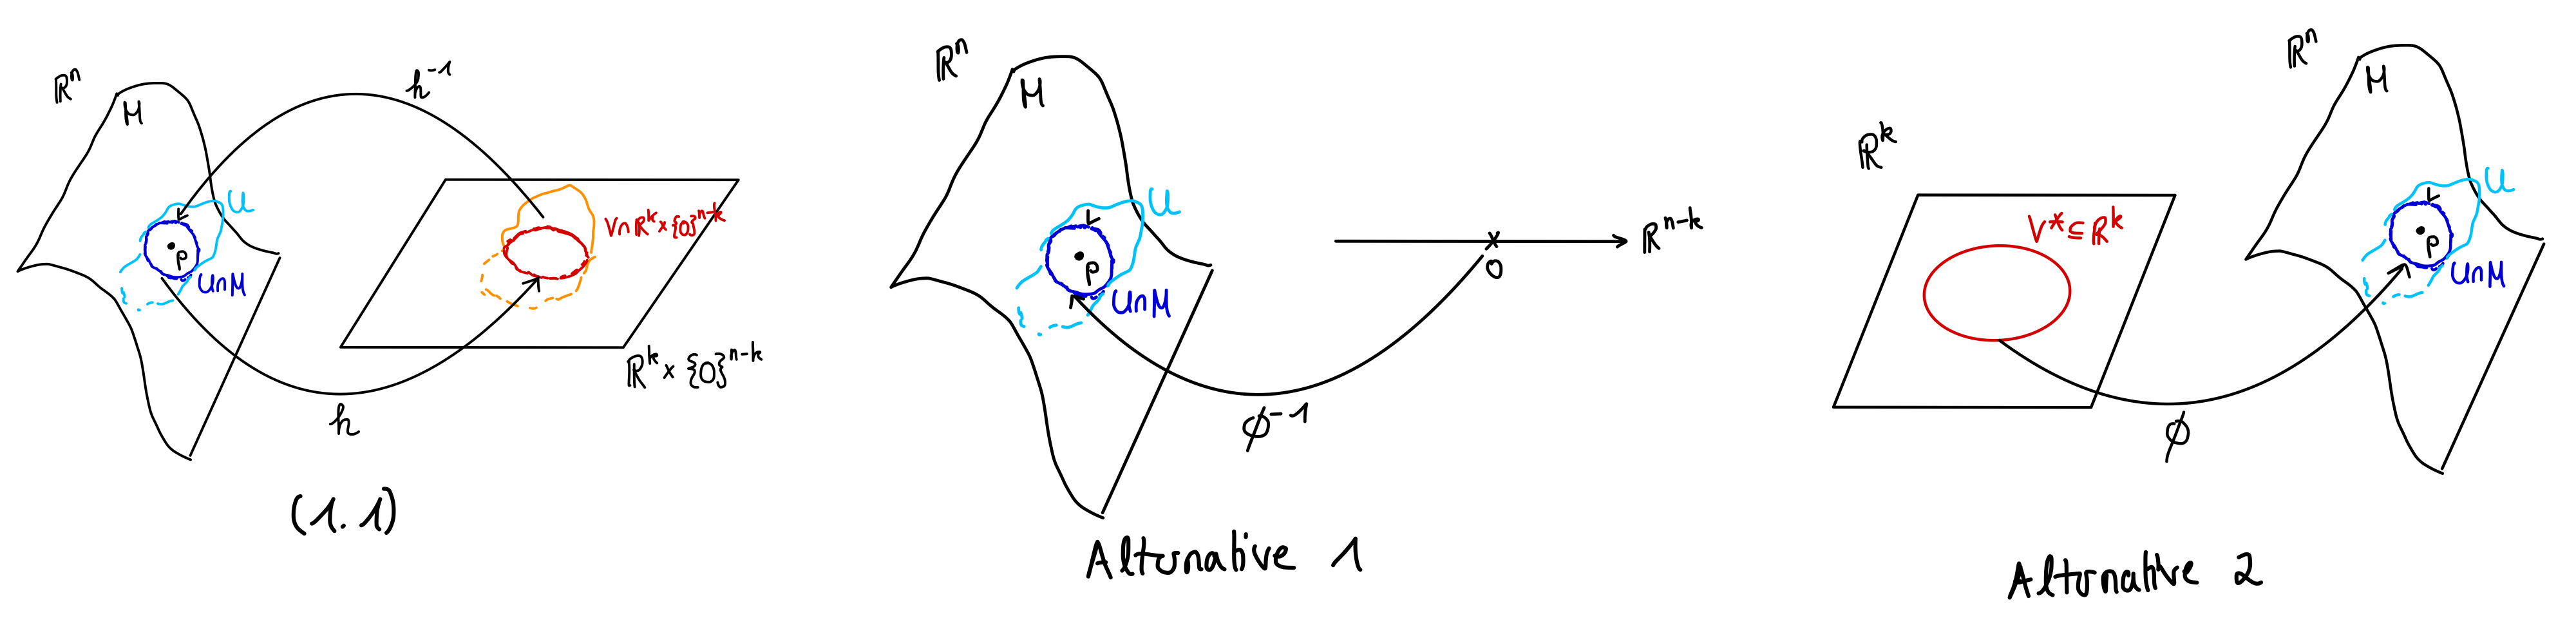
\includegraphics[width=0.9\linewidth]{Bilder/umf_def.png}
\caption{Die verschiedenen Definitionen von UMF.}
\end{figure}
Wir betrachten zwei Beispiele für Untermannigfaltigkeiten:
\begin{beispiele}{verschiedene Untermannigfaltigkeiten}
\begin{enumerate}
\item Betrachte die $k$-dim. Sphäre $\mathbb{S}^k := \{x \in \R^{k+1} | ||x||^2 = \sum_j x_j^2 = 1 \} \subseteq \R^{k+1}$. Wir definieren
\begin{align}
\psi: \R^{k+1} &\to \R \\
x &\mapsto 1-||x||^2 = 1 - \ip{x, x}.
\end{align}
Dann gilt für die Ableitung an $v \in \sph^k$ in Richtung $x$: $\diff \psi_x (v) = -2 \ip{x, v} \neq 0 \forall x \in \mathbb{S}^k$. Also hat das Differential vollen Rang und ist somit surjektiv. Um die Bedingung aus der Definition nachzuprüfen, geht man wie folgt vor: Sei $x \in \sph^k$. O.B.d.A. gilt $x_1 > 0$. Wir wählen $U := \{ x \in \R^{k+1} | x_1 > 0 \}$ und betrachten eine Funktion $h: U \to \R^k, (x_1, \dots, x_{k+1}) \mapsto (x_1 - \sqrt{1-\Sum{j, 2, k+1} x_j^2}, x_2, \dots, x_{k+1})$. Es gilt $\sum_j x_j^2 =1$, also $x_1^2 = 1-\Sum{j,2,k+1} x_j^2$. 
\item Sei $W \subseteq \R^k$ offen und $f: W \to \R^{n-k}$ eine glatte Abbildung, dann ist der \textbf{Graph von} $f$,
\begin{equation}
\graph f:= \{ (x, f(x) \in W \times \R^{n-k} \} \sub \R^k \times \R^{n-k},
\end{equation}
eine UMF der Dimension $k$ in $\R^n$.
Als Umgebung wählen wir $W \times \R^{n-k} \sub \R^n$ und als Diffeomorphismus $h: U \to \R^k \times \R^{n-k}, (x, y) \mapsto (x, y-f(x))$ respektive $\psi(x,y)=y-f(x)$.
\end{enumerate}
\begin{figure}[H]
\label{fig:graph}
\centering
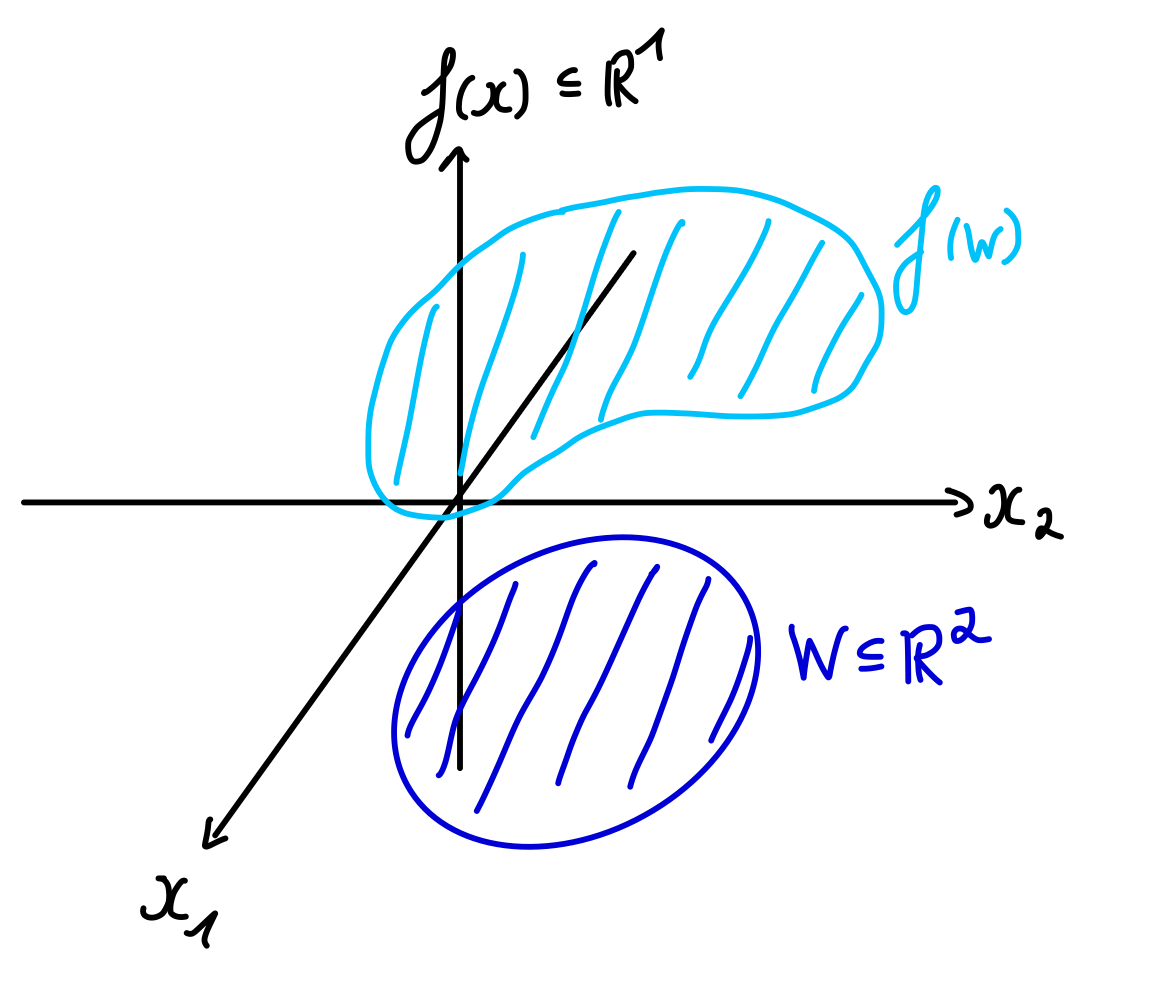
\includegraphics[width=0.2\linewidth]{Bilder/graph.png}
\caption{Der Graph einer Abbildung $f$.}
\end{figure}
\end{beispiele}
\begin{lemma}{Kartenlemma}{kartenlemma}
Sei $M \sub \R^n$ eine $k$-dim. UMF und $p \in M$.\\
Dann existiert eine Umgebung $U \sub \R^n$ von $p$ und eine offene Menge $W \sub \R^k$ sowie eine glatte Abbildung $\phi: W \to U$ mit folgenden Eigenschaften:
\begin{itemize}
\item $\forall y \in W$ hat $\diff \phi_y: \R^k \to \R^k$ maximalen Rang $k$.
\item $\phi$ ist injektiv mit $\phi(W) = U \cap M$.
\end{itemize}
\end{lemma}
\begin{beweis}
Ist $h: U \to V$ ein lokaler Diffeomorphismus wie in \ref{umfn}, können wir $W := \R^k \times \{ 0 \}^{n-k}$ und $\phi: h^{-1}|_W : W \to U \cap M$ betrachten.
\end{beweis}
Es gilt sogar, dass $\phi: W \to U \cap M$ ein Homöomorphismus ist.\\
\begin{theorem}{\textit{Umkehrsatz im} $\R^n$}{kleinerumkehrsatz}
Seien $U,V \sub \R^n$ offen, $p \in U$ und $F: U \to V$ glatt. Ist $F_{\ast,p}$ \textcolor{red}{invertierbar in} $p$, so existieren zusammenhängende Umgebungen $U_0 \sub U$ von $p$ und $V_0 \sub V$ von $F(p)$, sodass
\begin{equation}
F|_{U_0}: U_0 \to V_0
\end{equation} 
ein \textcolor{red}{Diffeomorphismus} ist.
\end{theorem}
\begin{theorem}{\textit{Satz von der impliziten Funktion}}{satzvonderimplizitenfunktion}
Sei $U \sub \R^n \times \R^n$ offen und seien $(x,y) = (x_1, \dots, x_n, y_1, \dots y_n)$ Standardkoordinaten auf $U$. Sei weiterhin $\Phi: U \to \R^k$ eine glatte Funktion, $(a,b) \in U$ und $c=\Phi(a,b)$. Wenn die Matrix
\begin{equation}
\left\{ \frac{\partial \Phi_i}{\partial y_j}(a,b)\right\}
\end{equation}
\textcolor{red}{nicht-singulär} ist, existieren offene Umgebungen $V_0 \sub \R^n$ von $a$, $W_0 \sub \R^k$ von $b$ und eine glatte Funktion $F: V_0 \to W_0$, sodass $\Phi^{-1}(x) \cap (V_0 \times W_0)$ der Graph von $F$ ist, also $\Phi(x,y)=c$ für $(x,y) \in V_0 \times W_0$ genau dann, wenn $y=F(x)$.
\end{theorem}
\begin{definition}{Topologische Mannigfaltigkeit}{topmfn}
Eine \textbf{topologische Mannigfaltigkeit (MFK) der Dimension} $k$ ist ein topologischer Raum $M$ mit folgenden Eigenschaften:
\begin{itemize}
\item $\forall p \in M$ existiert eine offene Umgebung $U$, die homöomorph zu einer offenen Menge $V \sub \R^k$ ist.
\item $M$ ist hausdorffsch.
\item $M$ besitzt eine abzählbare Basis.
\end{itemize}
\end{definition}
\begin{definition}{Hausdorffeigenschaft}{hausdorff}
Ein top. Raum $(X, \Ts)$ heißt \textbf{hausdorffsch}, wenn für alle $x,y \in X, x \neq y$ disjunkte offene Umgebungen $U \in \Ts$ von $x$ und $V \in \Ts$ von $y$ existieren.
\end{definition}
Die wichtigsten Beispiele von Hausdorffräumen sind metrische Räume (dort erfüllt der offene Ball die gewüschten Eigenschaften).
\begin{bemerkung}
Die Forderung der Hausdorffeigenschaft in \ref{topmfn} ist motiviert durch Beispiele folgender Art:\\
Sei $Y := \R \times \{0\} \sqcup \R \times \{1\}$. Wir betrachten die Äquivalenzrelation
\begin{equation}
(t, 0) \sim (s, 1) \iff t=s < 0.
\end{equation} 
Auf $X$ definieren wir eine Topologie: Wie haben Einbettungen
\begin{align}
\iota_0: \R \to X, \ &t \mapsto (t, 0) \\
\iota_1: \R \to X, \ &t \mapsto (t, 1)
\end{align}
und definieren $U \sub X$ als offen genau dann, wenn $\iota_0^{-1} (U)$ offen in $\R$ ist.
\end{bemerkung}
\begin{warning}
Der letzte Teil auf der Tafel wurde nicht mehr hochgeschoben, eine Ergänzung wäre nett.
\end{warning}
\begin{definition}{Basis}{topbasis}
Sei $(X, \cT)$ ein top. Raum. Eine \textbf{Basis} der Topologie $\cT$ ist eine Teilmenge $\beta \sub \cT$ mit der Eigenschaft, dass sich alle offenen $U \in \cT$ schreiben lassen als Vereinigung $U = \bigcup_{i \in I} B_i$ von $B_i \in \beta$.
\end{definition}
Wir sehen uns ein paar Beispiele an:
\begin{beispiele}{(abzählbare) Basen}
\begin{enumerate}
\item Sei $(X, d)$ ein metrischer Raum. Dann bilden die offenen Bälle eine Basis der Topologie.
\item Der $\R^n$ besitzt eine \textit{abzählbare} Basis. Dazu betrachtet man beispielsweise nur Bälle $\Bs_r(x)$ mit $r, x \in \Q$. Jeder Teilraum erbt diese Eigenschaft.
\end{enumerate}
\end{beispiele}
\begin{definition}{Parakompaktheit}{parakomp}
Ein top. Raum $X$ heißt \textbf{parakompakt}, wenn jede offene Überdeckung von $X$ eine lokal endliche \textit{Verfeinerung} aufweist.\\
Genauer: Ist $\{U_\alpha\}_{\alpha \in A}$ eine beliebige offene Überdeckung von $X$, so existiert eine offene Überdeckung $\{V_\beta \}_{\beta \in B}$ mit zwei Eigenschaften:
\begin{itemize}
\item $\forall \beta \in B \exists \alpha \in A: V_\beta \sub U_\alpha$
\item $\forall x \in X$ existiert ein offenes $U \sub X$ , sodass $\{ \beta \in B | V_\beta \cup U \neq \emptyset \}$ endlich ist.
\end{itemize}
\begin{figure}[H]
\label{fig:parakomp}
\centering
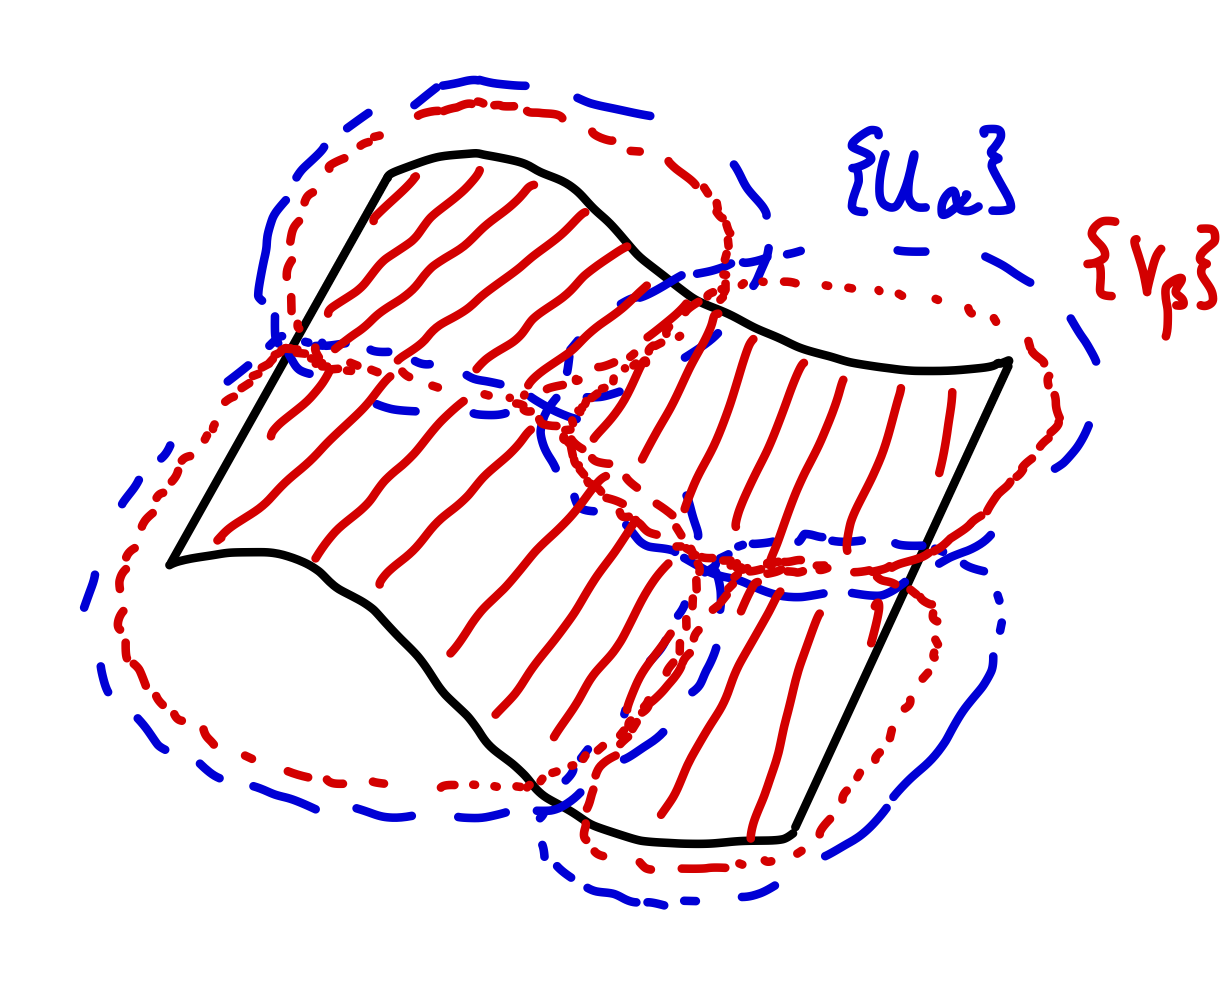
\includegraphics[width=0.2\linewidth]{Bilder/parakompakt.png}
\caption{Eine parakompakte MFK.}
\end{figure}
\end{definition}
\begin{satz}{Parakompaktheit top. MFN}{parakompmfn}
Jede top. MFK ist parakompakt.
\end{satz}
\begin{definition}{\textit{zusammenhängend}}{zusammenhängend}
Sei $X$ ein topologischer Raum. $X$ heißt \textbf{zusammenhängend}, falls er sich nicht in zwei offene, disjunkte, nicht-leere Teilmengen zerlegen lässt.\\
Anders formuliert: Sind $U,V \sub X$ offen, nicht-leer und gilt $X = U \cup V$, so folgt $U \cap V \neq \emptyset$.
\end{definition}
\begin{definition}{\textit{wegzusammenhängend}}{wegzusammenhängend}
Ein topologischer Raum $X$ heißt \textbf{wegzusammenhängend}, falls zu je zwei Punkten $x,y \in X$ eine stetige Abbildung
\begin{equation}
c: [0,1] \to X
\end{equation}
mit $c(0)=x$ und $c(1)=y$ existiert.
\end{definition}
\subsection{Glatte Mannigfaltigkeiten}
\label{subsec: smoothmfn}
\begin{definition}{Karte}{karte}
Sei $X$ eine top. MFK.\\
Eine \textbf{Karte um} $p \in X$ ist eine offene Umgebung $U \sub X$ von $p$ und eine Abbildung 
\begin{equation}
\phi: U \to \R^n,
\end{equation}
die $U$ \textit{homöomorph} auf eine offene Teilmenge $V \in \R^n$ abbildet.
\end{definition}
\begin{definition}{(glatter) Atlas}{atlas}
Sei $X$ eine top. MFK.\\
Unter einem \textbf{Atlas von} $X$ versteht man eine Familie von Karten $(\phi_\alpha, U_\alpha)_{\alpha \in A}$ mit $\bigcup_{\alpha \in A} U_\alpha = X$.\\
Ein Atlas heißt \textbf{glatt}, wenn die Kartenwechselabbildungen glatte Abbildungen zwischen offenen Teilmengen des $\R^n$ sind.
\begin{figure}[H]
\label{fig:kartenwechsel}
\centering
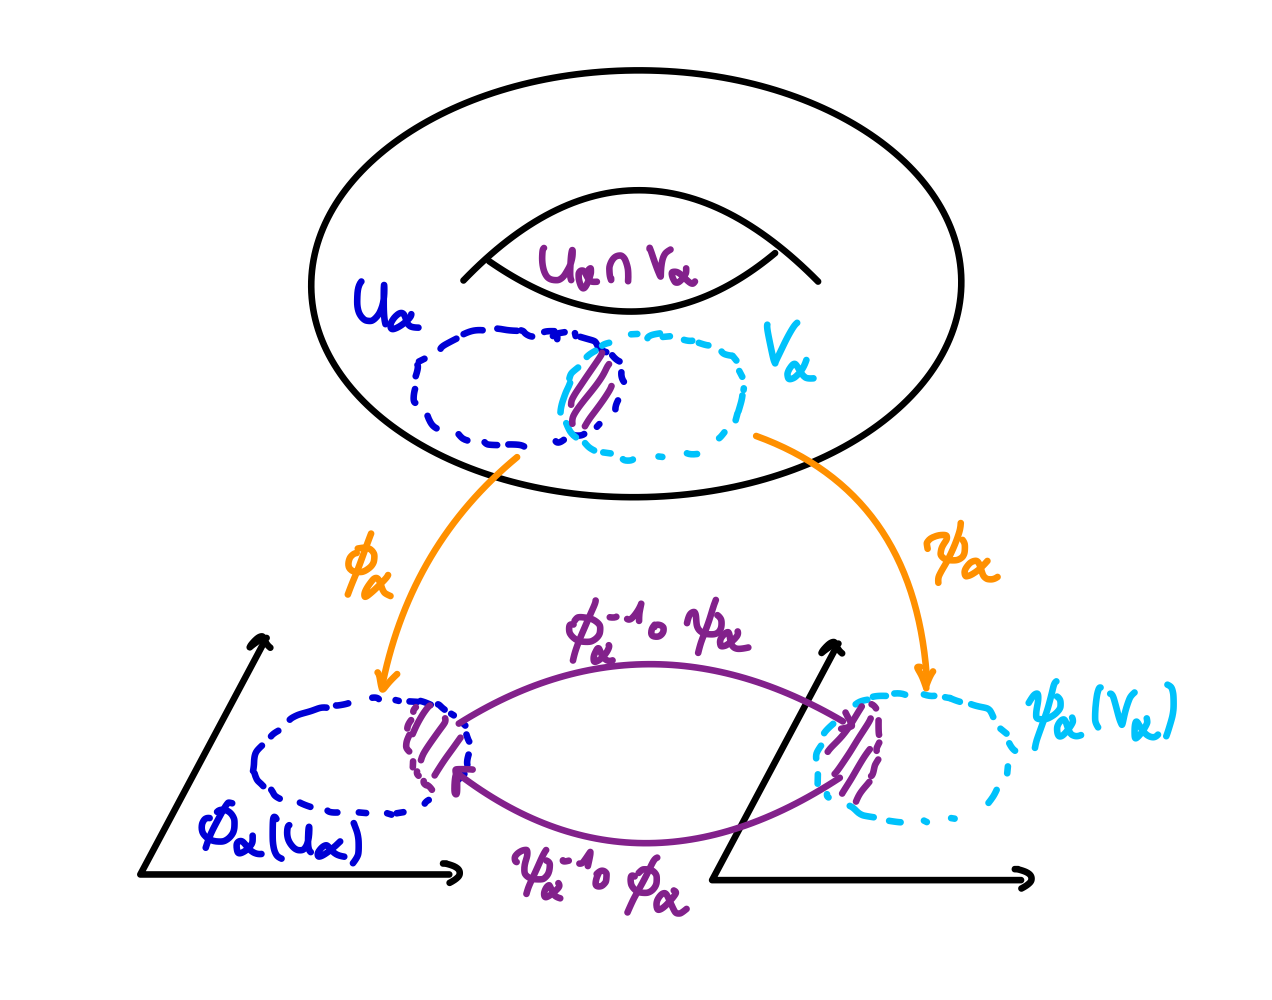
\includegraphics[width=0.3\linewidth]{Bilder/kartenwechsel.png}
\caption{Ein Atlas mit Kartenwechselabbildung.}
\end{figure}
\end{definition}
Wir sehen uns ein Beispiel anhand der schon bekannten $n$-Sphäre an:
\begin{beispiel}{Stereographische Projektion} \\
Sei $X := \sph^n \sub \R^{n+1} \cong \R^n \times \R$. Wir definieren die \textbf{stereographische Projektion} durch:
\begin{align}
\sigma_\pm : \sph^n \exc (0, 0, \dots, \pm 1) & \to \R^n \\
(x_1, \dots, x_{n+1}) & \mapsto \left( \frac{x_1}{1 \mp x_{n+1}}, \dots , \frac{x_n}{1 \mp x_{n+1}} \right)
\end{align} 
Nachrechnen zeigt, dass die Umkehrabbildungen in der Tat durch
\begin{align}
\phi_\pm : \R^n &\to \sph^n \\
y &\mapsto \left( \frac{2y}{1+||y||^2}, \pm \frac{||y||^2 - 1}{||y||^2 + 1}\right)
\end{align}
gegeben sind. Die Kartenübergänge
\begin{equation}
\sigma_\mp \circ \phi_\pm: \R^n \exc \{0\} \to \R^n \exc \{0\} 
\end{equation}
sind durch $y \mapsto \frac{y}{||y||^2}$ gegeben.\\
Auch andere Karten sind möglich:
Betrachte $U_i^\pm := \{ x \in \sph^n | x_i \gtrless 0 \}$ und 
\begin{align}
\psi_i^\pm: U_i^\pm &\to \R^n \\
(x_1, \dots, x_{n+1}) &\mapsto (x_1, \dots, \hat{x}_i, \dots, x_n)
\end{align}
mit Umkehrabbildung:
\begin{align}
\left( \psi_i^\pm \right)^{-1}: \D^n &\to \sph^n \\
(y_1, \dots, y_{n}) &\mapsto (y_1, \dots, y_{i-1}, \pm \sqrt{1-||y||^2}, y_i, \dots, y_n).
\end{align}
\begin{figure}[H]
\label{fig:sphere}
\centering
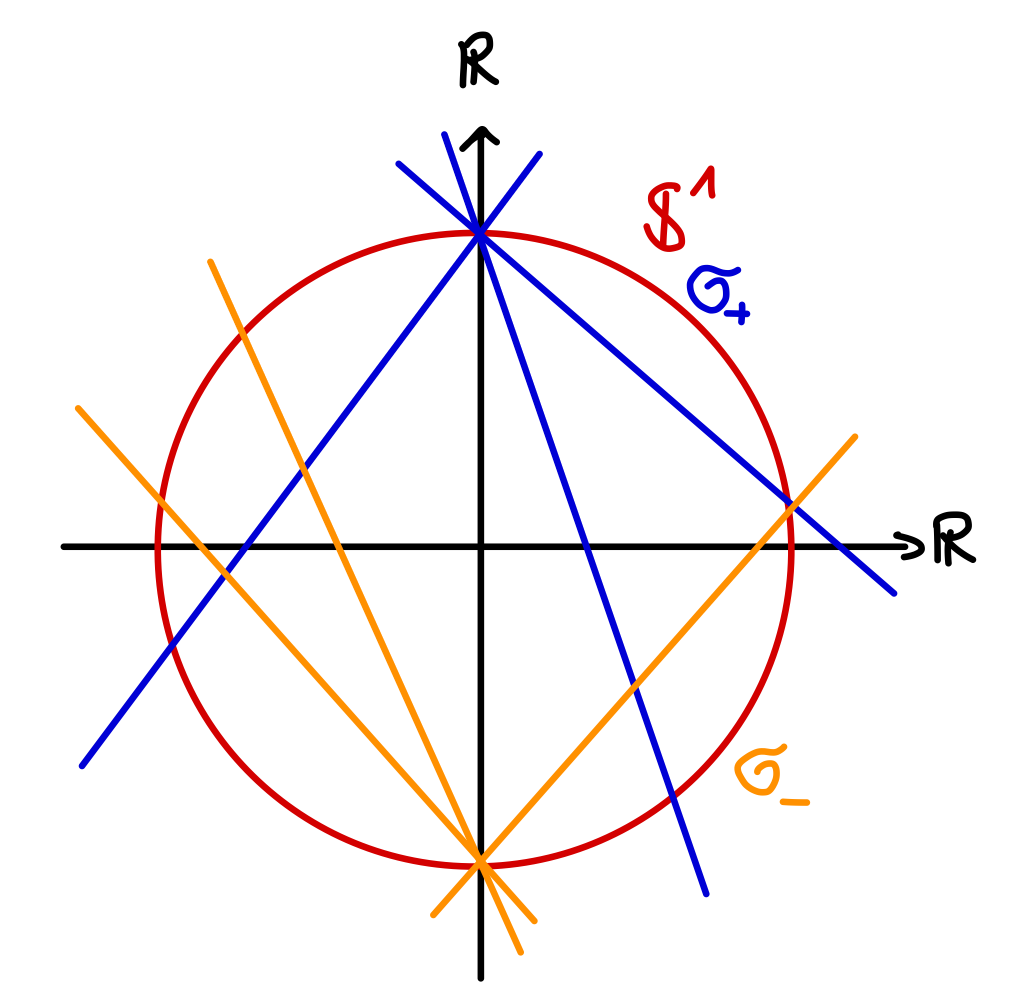
\includegraphics[width=0.2\linewidth]{Bilder/stereograph.png}
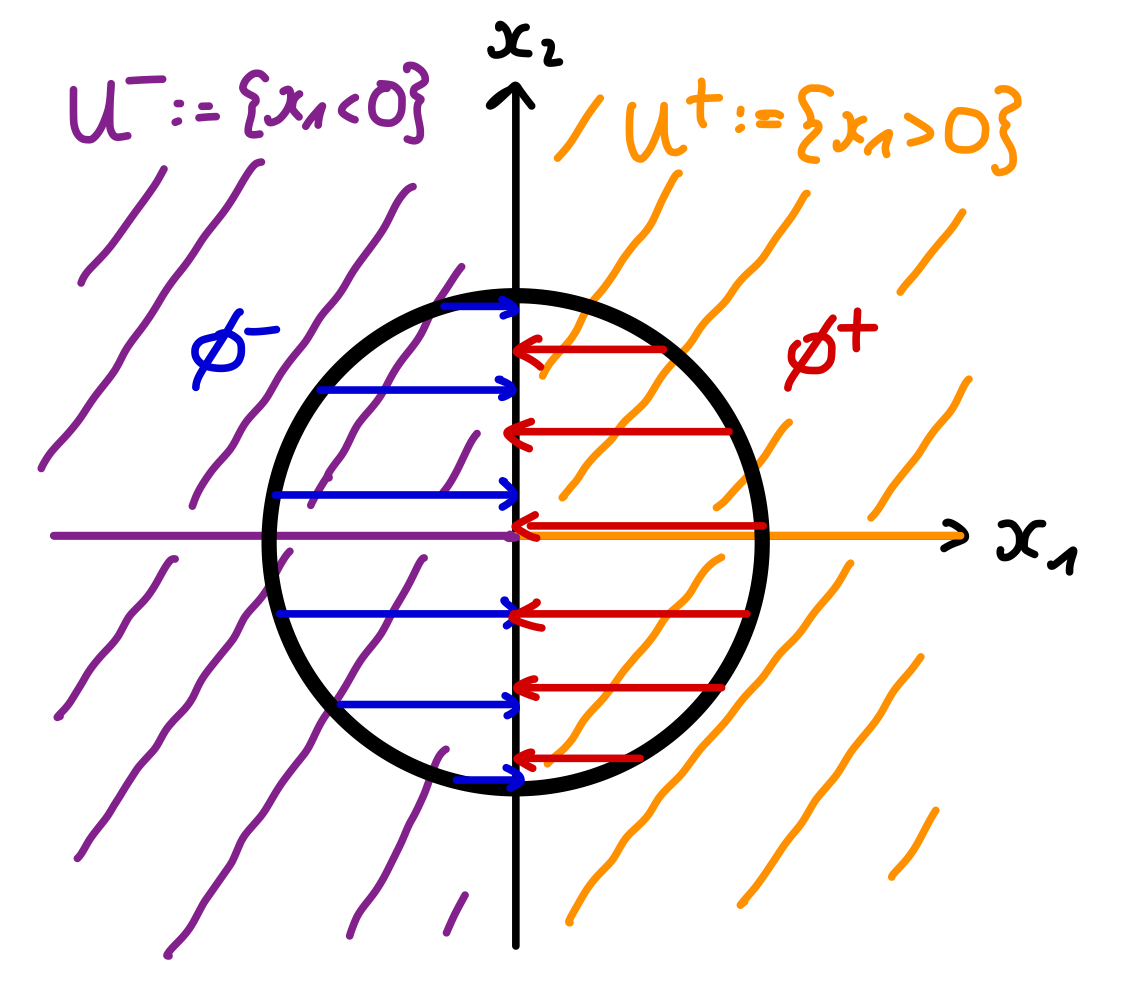
\includegraphics[width=0.2\linewidth]{Bilder/sphereproj.png}
\caption{Zwei Karten für $\sph^2$.}
\end{figure}
\end{beispiel}
\begin{definition}{äquivalente Atlanten}{äquivat}
Sei $X$ eine top. MFK. Zwei glatte Atlanten $\Af_1$ und $\Af_2$ heißen \textbf{äquivalent}, in Zeichen $\Af_1 \sim \Af_2$, wenn die Vereinigung $\Af_1 \cup \Af_2$ auch ein glatter Atlas ist.
\end{definition}
\begin{definition}{glatte Mannigfaltigkeit}{glattmfn}
Eine \textbf{glatte Struktur} auf einer top. MFK $X$ ist eine Äquivalenzklasse glatter Atlanten.\\
Eine \textbf{glatte MFK} ist eine top. MFK mit einer gewählten glatten Struktur.
\end{definition}
\begin{bemerkung}
Die für $\sph^n$ betrachteten Atlanten sind äquivalent, beschreiben also die gleiche glatte Struktur.
\end{bemerkung}
Wir betrachten dafür einige Beispiele:
\begin{beispiele} Einige glatte Strukturen
\begin{enumerate}
\item Die Karte $\id_{\R^n}: \R^n \to \R^n$ macht den $\R^n$ zu einer glatten MFK.
\item Offene Teilmengen von glatten MFKn sind wieder glatte MFKn, da sie die glatte Struktur der umgebenden MFK erben. Sei $O \sub M$ offen und $\phi: U \to \R^n$ eine Karte für $M$. Dann ist $\phi |_{O \cap U}: O \cap U \to \R^n$ eine Karte für $O$.
\item Betrachte $\text{GL}(n, \R) \sub \text{Mat}(n, \R) \cong \R^{n^2}$. Als Urbild von $\R \exc \{ 0 \} \sub \R$ unter $\text{det}: \text{Mat}(n, \R) \to \R$ ist $\text{GL}(n, \R)$ offen in $\text{Mat}(n, \R)$.
\item Jede $k$-dim. UMF des $\R^n$ ist eine glatte $k$-dim. MFK.
\item Seien $M_1$ und $M_2$ glatte MFK. Dann ist das Produkt $M_1 \times M_2$ wieder eine glatte MFK. Betrachte dazu Karten $\phi_{1,2}: U_{1,2} \to \R^{n_{1,2}}$ von $M_1$ respektive $M_2$. Dann ist $\phi_1 \times \phi_2: U_1 \times U_2 \to \R^{n_1 + n_2}$ eine Karte für $M_1 \times M_2$.
\end{enumerate}
\end{beispiele}
\begin{bemerkung}Andere Definition glatter MFK \\
Sei $X$ eine Menge und seien $U_\alpha \sub X$ endlich viele Teilmengen mit $\bigcup_\alpha U_\alpha = X$. Seien $\phi_\alpha : U_\alpha \to V_\alpha \sub \R^n$ Bijektionen. Dann definieren wir eine Topologie wie folgt: $U \in X$ ist offen genau dann, wenn $\forall \alpha \in A: \phi_\alpha (U \cap U_\alpha) \sub \R^n$ offen sind.\\
Ist diese Topologie hausdorffsch, ist $X$ eine top. MFK. Sind die Kartenübergänge glatt, erhalten wir die Struktur einer glatten MFK auf X.
\begin{figure}[H]
\label{fig:glattetopmfk}
\centering
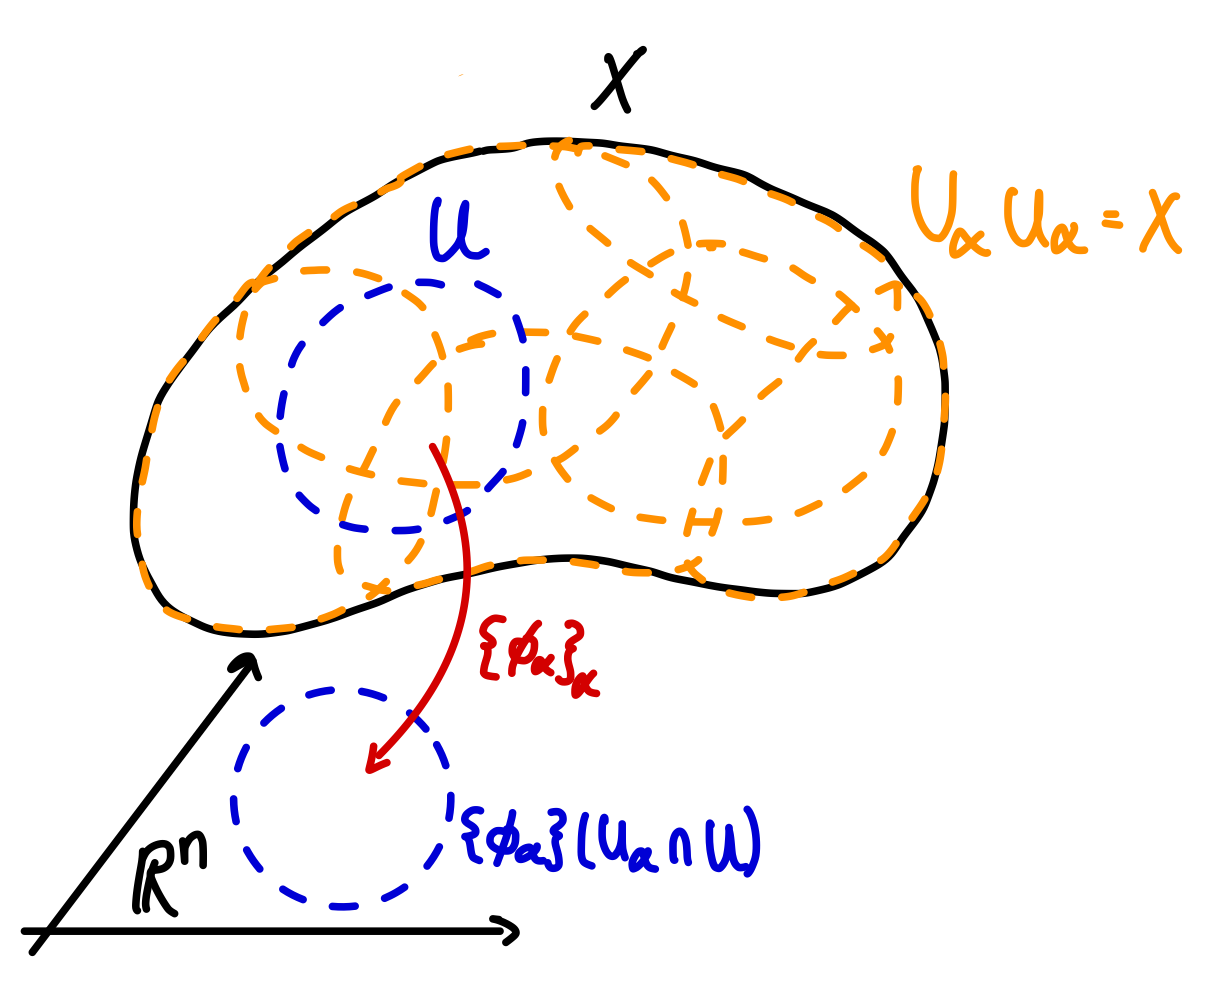
\includegraphics[width=0.25\linewidth]{Bilder/glattetopmfk.png}
\caption{Eine topologische MFK mit Karte in der von den Karten induzierten Topologie.}
\end{figure}
\end{bemerkung}
\begin{beispiel}Der reell projektive Raum \\
Der \textbf{reell projektive Raum} $\R P^n$ besteht aus allen Ursprungsgeraden im $\R^{n+1}$.\\
Für $l \in \R P^n$ betrachten wir 
\begin{align}
U_l :=& \{ g \in \R P^n | \pi_{l|g}: g \to l \ \text{ist ein Isomorphismus} \}\\
=& \{ g \in \R P^n | g \nsubseteq l^\perp \}
\end{align}
Damit ist jede Gerade $g \in U_l$ Graph einer linearen Abbildung $A_g: l \to l^\perp$. Damit bekommen wir die Bijektion $\phi_l : U_l \to L(l, l^\perp) \cong L(\R, \R^n) \cong \R^n$. Der $\R P^n$ erhält so eine Überdeckung durch $\{U_i\}_{i=1}^{n+1}$ mit $U_i \equiv U_{\R_{l_i}}$.
\begin{figure}[H]
\label{fig:sphere}
\centering
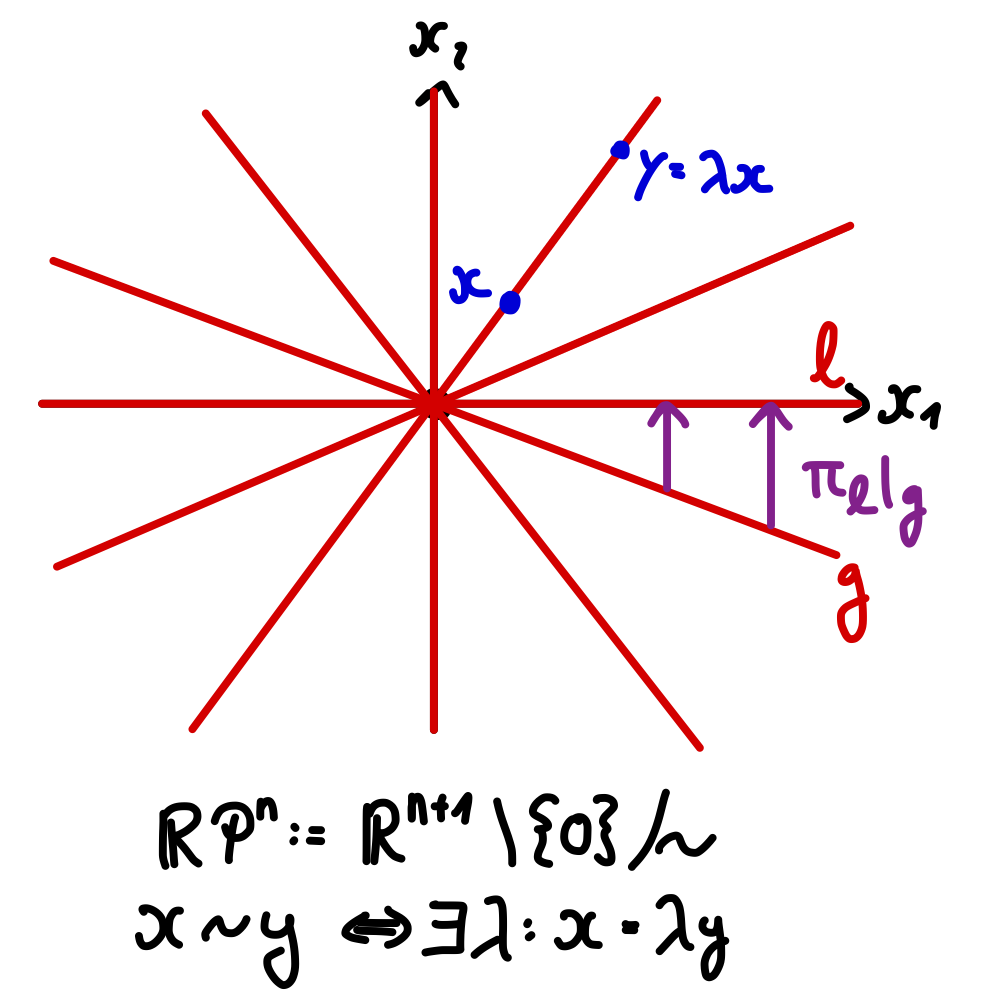
\includegraphics[width=0.25\linewidth]{Bilder/rpn.png}
\caption{Zu sehen ist der $\R P^1$. Die Graphik zeigt, warum man keinen Isomorphismus findet, wenn $l \perp g$ ist: Alle Punkte auf $l$ würden auf einen Punkt auf $g$ abgebildet werden.}
\end{figure}
\end{beispiel}
\begin{satz}{Glatter Atlas für $\R P^n$}{rpnglatt}
Seien $\phi_i$ und $U_i$ wie oben. Dann ist $\Af = \{ (\phi_i, U_i) | 1 \leq i \leq n+1 \}$ ein glatter Atlas für $\R P^n$.
\end{satz}
\begin{beweis}
Bezüglich der Standardkoordinaten ist die Abbildung gegeben durch
\begin{align}
\phi_i : U_i & \to \R^n \\
\R v & \mapsto \left( \frac{v_1}{v_i}, \dots, \hat{\frac{v_i}{v_i}}, \dots, \frac{v_{n+1}}{v_i}\right)
\end{align}
mit der Umkehrabbildung
\begin{align}
\phi_i^{-1}: \R^n &\to U_i \sub \R P^n \\
(y_1, \dots, y_n) &\mapsto \R \cdot (y_1, \dots, y_{i-1}, 1, y_i, \dots, y_n)
\end{align}
Ein Kartenübergang $\phi_j \circ \phi_i ^{-1} : \phi_i (U_i \cap U_j) \to \phi_j (U_i \cap U_j)$ hat dann für $j < i$ die Gestalt:
\begin{align}
\phi_i (U_i \cap U_j) &= \{ y \in \R^n | y_j \neq 0 \} \\
\phi_j (U_i \cap U_j) &= \{z \in \R^n | z_{i-1} \neq 0 \}
\end{align}
Für den Kartenübergang findet man:
\begin{equation}
\phi_j \circ \phi_i^{-1} (y_1, \dots, y_n) = \phi_j (y_1, \dots, y_{i-1}, 1, y_i, \dots, y_n) = \left(\frac{y_1}{y_j}, \dots, \hat{\frac{y_i}{y_j}},\dots, \frac{y_{i-1}}{y_j}, \frac{1}{y_j}, \frac{y_{i}}{y_j}, \dots, \frac{y_{n}}{y_j} \right)
\end{equation}
Da auf dem Definitionsbereich $y_j \neq 0$ gilt, ist der Kartenübergang und damit auch $\Af$ glatt.
\end{beweis}
\begin{korollar}{}{}
Mit den obigen Karten ist $\R P^n$ eine \textit{glatte MFK}.
\end{korollar}
\begin{bemerkung}Grassman-MFK\\
Die Unterräume $G_{k, n} := \{ k \text{-dim. linearer UR des} \ \R^n \}$ erhalten auf analoge Weise die Struktur einer MFK und werden \textbf{Grassman-Mannigfaltigkeiten} genannt.
\end{bemerkung}
Sei $M$ eine top. MFK. Für Dimensionen $n \leq 3$ gibt es für $M$ immer eine eindeutige glatte Struktur. Ab Dimension $n > 3$ ist dies nicht mehr gegeben.
\begin{definition}{glatte Abbildung}{glattfkt}
Seien $M_1$ und $M_2$ glatte MFKn. Eine Abbildung $f: M_1 \to M_2$ heißt \textbf{glatt}, wenn $f$ stetig ist und für alle Karten $(\phi, U)$ von $M_1$ und $(\psi, V)$ von $M_2$ mit $f^{-1}(V) \cap U \neq \emptyset$ die Abbildung
\begin{equation}
\psi \circ f \circ \phi^{-1}: \phi(f^{-1}(V) \cap U) \to \psi (V)
\end{equation}
eine glatte Abbildung zwischen offenen Teilmengen des $\R^{n_1}$ und $\R^{n_2}$ ist.
\begin{figure}[H]
\label{fig:sphere}
\centering
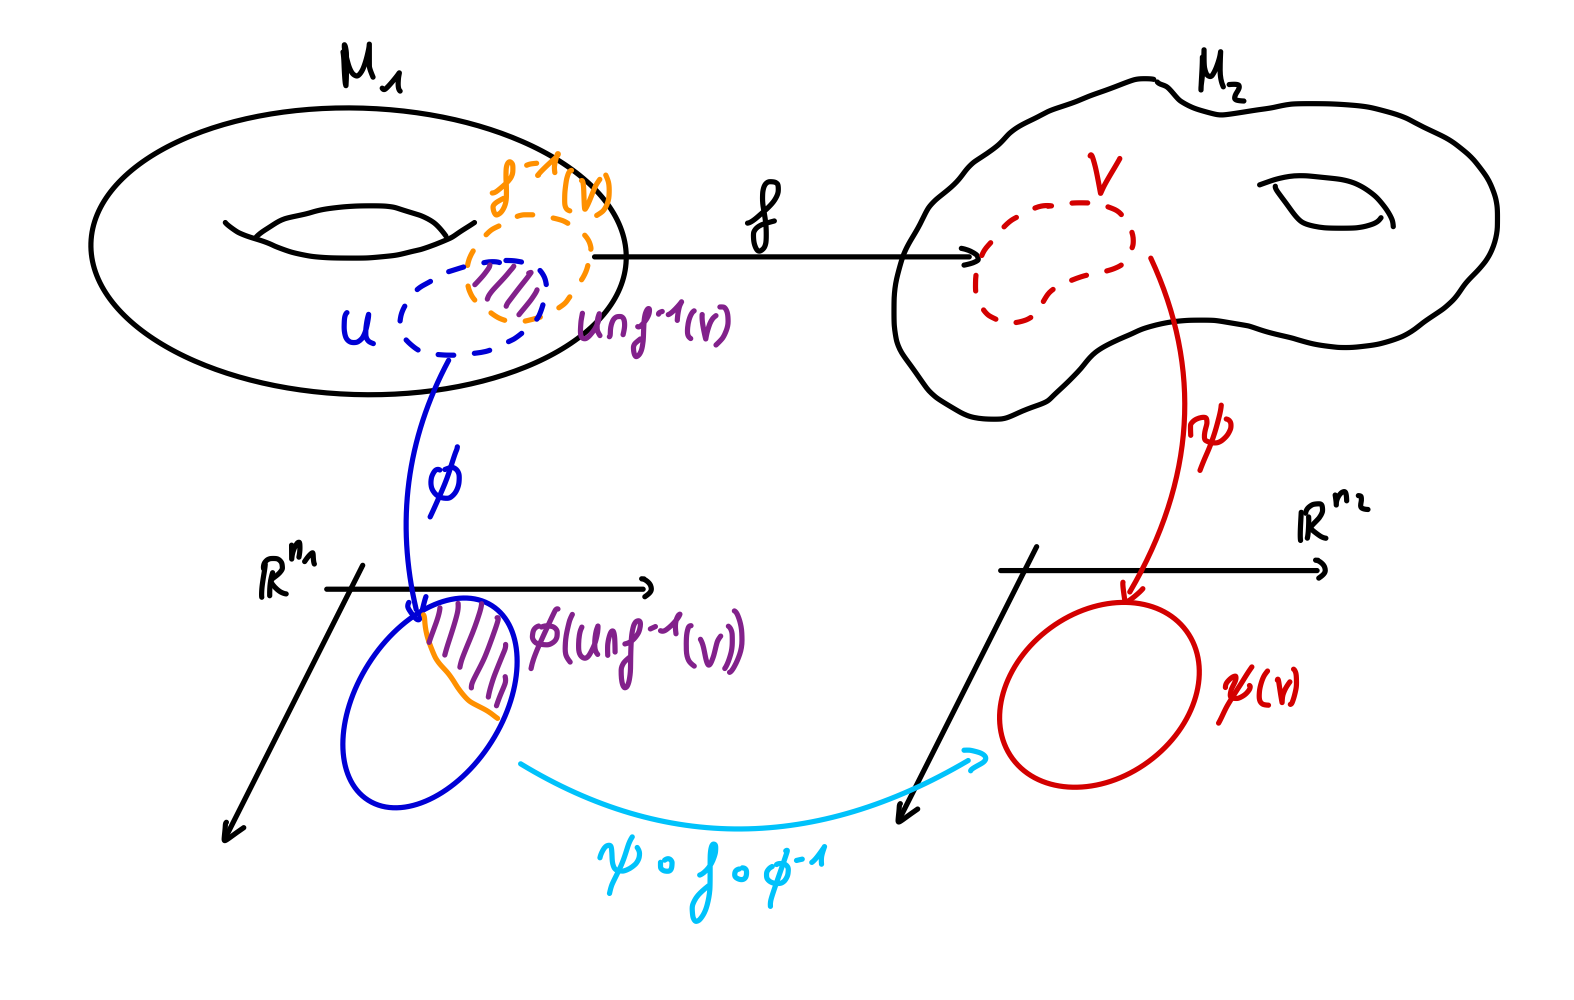
\includegraphics[width=0.3\linewidth]{Bilder/glatteabb.png}
\caption{Kartenwechsel mit einer glatten Abbildung.}
\end{figure}
\end{definition}
\begin{bemerkungen}Spezialfälle glatter Abbildungen\\
\begin{enumerate}
\item Eine Funktion $f: M \to \R$ ist glatt, wenn für alle Karten die Abbildung $f \circ \phi^{-1}: \phi(U) \to \R$ glatt ist.
\item Ist $M \sub \R^n$ eine UMF, so ist $f: M \to \R^k$ genau dann glatt, wenn es zu jedem Punkt $p \in M$ eine offene Umgebung $U \sub \R^n$ und eine glatte Funktion $F: U \to \R^k$ gibt, sodass $f|_{U \cap M} = F|_{U \cap M}$ ist.
\end{enumerate}
\end{bemerkungen}
\begin{definition}{(glatter) Diffeomorphismus}{diffeomorph}
Eine glatte Abbildung $f: M_1 \to M_2$ zwischen glatten MFK $M_1, M_2$ heißt \textbf{(glatter) Diffeomorphismus}, falls gilt:
\begin{itemize}
\item $f$ ist bijektiv.
\item Die Umkehrabbildung $f^{-1}: M_2 \to M_1$ ist ebenfalls glatt.
\end{itemize}
\end{definition}
Für jede glatte MFK $M$ bilden die Diffeomorphismen $M \to M$ eine Gruppe $\diffm (M)$.
\begin{beispiele}
\begin{enumerate}
\item Die Antipodenabbildung
\begin{align}
A: \sph^n &\to \sph^n \\
p &\mapsto -p
\end{align}
ist ein glatter Diffeomorphismus mit $A^{-1} = A$.
\item Für jede MFK $M$ ist die Abbildung
\begin{align}
S: M \times M &\to M \times M \\
(x, y) &\mapsto (y, x)
\end{align}
ein Diffeomorphismus.
\item Die Exponentialabbildung
\begin{align}
\exp: \R &\to \sph^1\\
t &\mapsto (\cos t, \sin t)
\end{align}
ist glatt und \textit{lokal} ein Diffeomorphismus. Das heißt, dass $\exp$ bei Einschränkung auf ein hinreichend kurzes Intervall (Länge $<2\pi$) ein Diffeomorphismus aufs jeweilige Bild ist.
\end{enumerate}
\end{beispiele}
\begin{definition}{glatte Wirkung}{glattewirk}
Eine \textbf{glatte Wirkung} einer Gruppe $G$ auf einer glatten MFK $M$ ist ein \textit{Gruppenhomomorphismus}
\begin{align}
G &\to \diffm (G)\\
g &\mapsto \phi_g: M \to M
\end{align}
mit $\phi_{g_1} \circ \phi_{g_2} = \phi_{g_1g_2}$ und $\phi_{g^{-1}}=(\phi_g)^{-1}$.
\end{definition}
$G \times M \to M, \ (g, x) \mapsto \phi_g(x)$ soll glatt sein, wenn es sich bei $G$ um eine \textit{Lie-Gruppe} handelt.
\begin{beispiele}glatte Wirkungen \\
\begin{enumerate}
\item Die Gruppe $\Z$ wirkt direkt auf $\R$ durch Translationen: Für $k \in \Z$ betrachten wir $\phi_k: \R \to \R, \ t \mapsto \phi_k(t)=t+k$.
\item Die Gruppe $\so{2}$ wirkt auf $\R^2$, wobei der Einheitskreis $\sph^1 \sub \R^2$ invariant bleibt.\\
Sei $A \in \so{2}$ mit $A \neq \id$ und $G_A \sub \so{2}$ die von $A$ erzeugte Untergruppe. Wir unterscheiden zwei Fälle:
\begin{itemize}
\item $A$ ist eine Drehung um einen Winkel $2 \pi \cdot \frac{p}{q}$ mit $\text{ggT} (p,q) = 1$. Dann ist $G_A$ eine \textit{zyklische} Untergruppe der Ordnung $q$.
\item $A$ ist eine Drehung um ein irrationales Vielfaches von $\pi$. Dann ist die Zuordnung $k \mapsto A^k$ injektiv und jede Bahn ist dicht in $\sph^1$.
\end{itemize}
\end{enumerate}
\end{beispiele}
\begin{definition}{freie Wirkung}{freiewirk}
Eine Gruppenwirkung heißt \textbf{frei}, falls für alle $g \in G$ mit $g \neq e$ der Diffeomorphismus $\phi_g: M \to M$ keine \textit{Fixpunkte} hat.
\end{definition}
Man kann zeigen, dass gilt:
\begin{satz}{glatte Struktur und Wirkung}{glattstrukwirk}
Sei $G$ eine endliche Gruppe, die glatt und frei auf einer glatten MFK $M$ wirkt.\\
Dann hat der Quotientenraum $\quotient{M}{G}$ eine eindeutige glatte Struktur, sodass die Projektion
\begin{equation}
\pi: M \to \quotient{M}{G}
\end{equation}
ein lokaler Diffeomorphismus ist.
\end{satz}
\begin{beispiel}Der Linsenraum\\
Seien $p, q \in \N$ teilerfremd mit $q>1$. Dann wirkt $G=\Z_q$ auf $\sph^3 \sub \C^2$ mit dem Erzeuger 
\begin{equation}
\sigma_{p,q} (z_1, z_2)= \left( \exp\left(\frac{2\pi i}{q}\right)z_1, \exp\left(\frac{2\pi i p}{q} \right)z_2\right).
\end{equation}
Der Quotientenraum heißt \textbf{Linsenraum} $\text{L}(p,q)$.
\end{beispiel}
\subsection{Tangentialräume}
\label{subsec:tangentspace}
Im Folgenden wollen wir mehrere Zugänge zu Tangentialräumen diskutieren.\\
Allgemein ist der Tangentialraum $T_pM$ an eine UMF $M \sub \R^n$ im Punkt $p \in M$ ein affiner Unterraum des $\R^n$, der $M$ an diesem Punkt bestmöglich approximiert. In der Analysis identifizieren wir diesen oft mit dem zugehörigen linearen Unterraum. Wir wollen aber den Fußpunkt weiterhin festhalten. \\
Den Tangentialraum an $\R^n$ im Punkt $p \in \R^n$ schreiben wir als $T_p\R^n := \{(p, \xi) | \xi \in \R^n \}$.
Seien $U \sub \R^n$ und $V \sub \R^m$ offen sowie $f: U \to V$ glatt. Dann kann für $p \in U$ die Ableitung $\diff f_p: \R^n \to \R^m$ als lineare Abbildung
\begin{align}
f_{\ast, p}: T_pU &\to T_{f(p)}V \\
(p, \xi) &\mapsto f_{\ast, p}(p, \xi) = (f(p), \diff f_p(\xi))
\end{align}
auffassen. Die Abbildung $f_{\ast, p}$ heißt \textbf{Differential} oder \textbf{Pushforward von} $f$ \textbf{in} $p$.
\begin{figure}[H]
\label{fig:sphere}
\centering
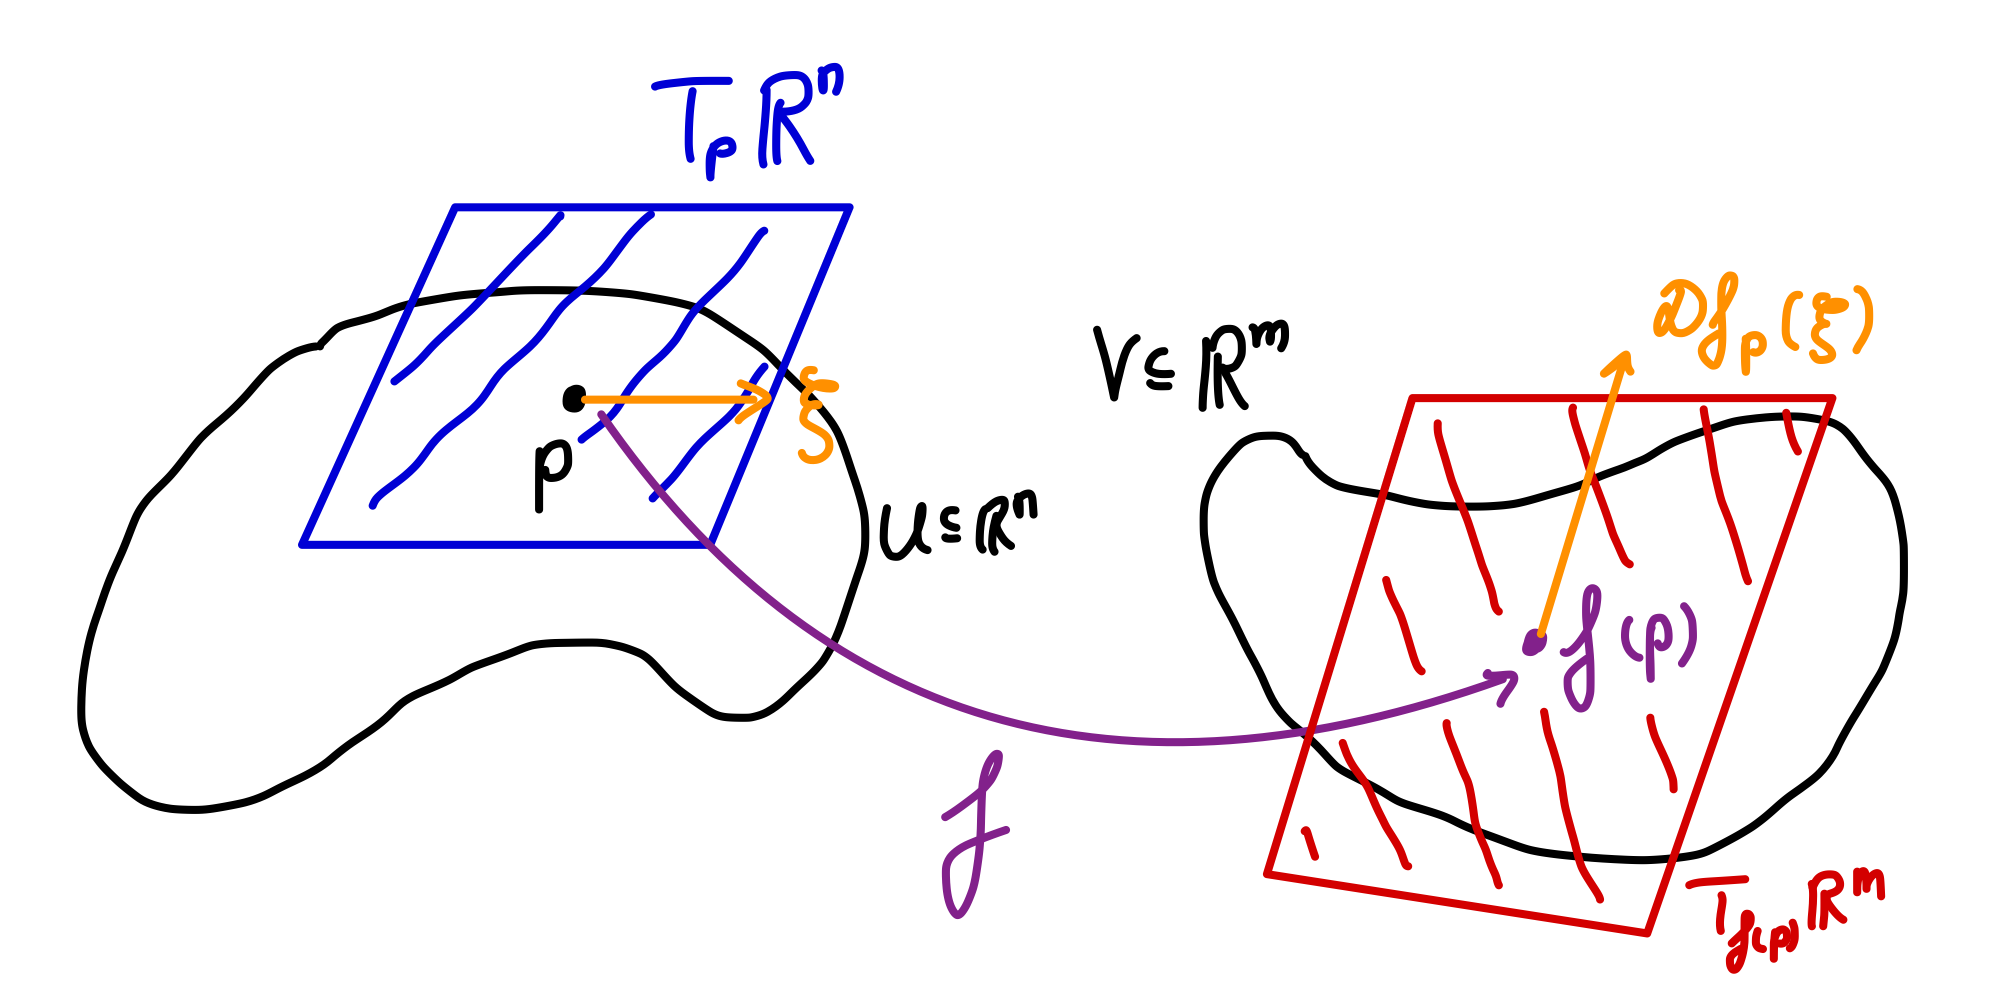
\includegraphics[width=0.3\linewidth]{Bilder/differentialrn.png}
\caption{Das Differential für offene Teilmengen des reellen Raums.}
\end{figure}
\begin{bemerkungen}Kartenwechsel und Differentiale\\
Sei $M$ eine $k$-dim. MFK und $p \in M$. Betrachte die Karten $\phi_1: U_1 \to V_1 \sub \R^k, \ \phi_1(p)=x_1$ und $\phi_2: U_2 \to V_2 \sub \R^k, \ \phi_2(p)=x_2$. Dann ist das Differential des Kartenübergangs
\begin{align}
(\phi_2 \circ \phi_1^{-1})_{\ast, x_1} : T_{x_1}\R^k &\to T_{x_2} \R^k\\
(x_1, \xi) &\mapsto (x_2, \diff (\phi_2 \circ \phi_1^{-1})_{x_1}(\xi))
\end{align}
ein \textit{linearer Isomorphismus}.
\end{bemerkungen}
\begin{definition}{Äquivalenz von Karten}{equivatlant}
Sei $M$ eine glatte MFK durch den Atlas $\Af$. Betrachte
\begin{equation}
\{(\phi, v) | \phi: U \to V \sub \R^k \ \text{ist Karte in} \ \Af \ \text{mit} \ p \in U, v \in T_{\phi(p)}\R^k \}
\end{equation}
mit der Äquivalenzrelation $(\phi, v) \sim_p (\psi, w) \iff w = (\psi \circ \phi^{-1})_{\ast, \phi(p)}(v)$. Transitivität erhalten wir durch die Kettenregel. Zwei Karten heißen \textbf{äquivalent}, wenn sie unter $\sim_p$ äquivalent sind.
\begin{figure}[H]
\label{fig:tangentialvek1}
\centering
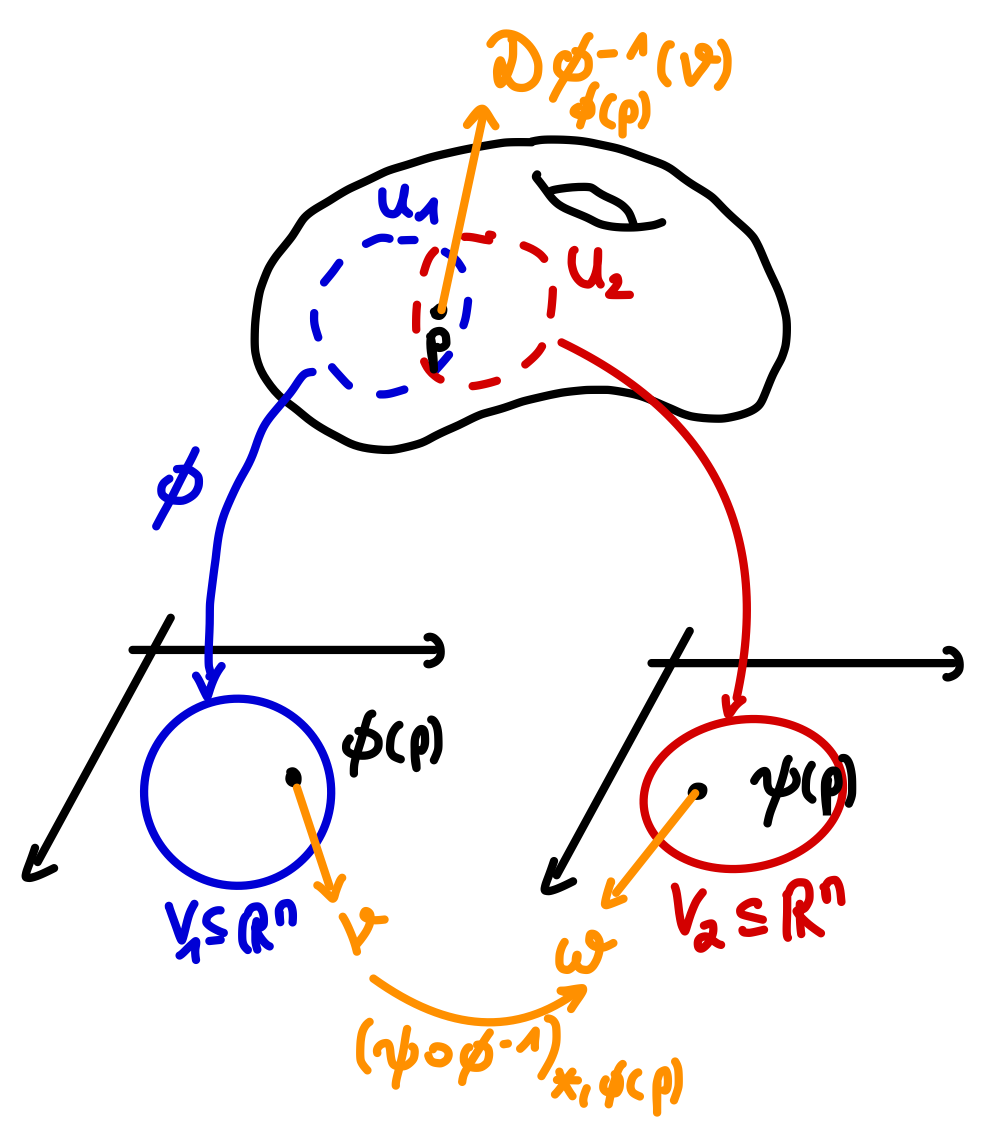
\includegraphics[width=0.2\linewidth]{Bilder/tangentialvek1.png}
\caption{Zwei äquivalente Karten unter $\sim_p$.}
\end{figure}
\end{definition}
\begin{bemerkung}
Für jede Karte $\phi: U \to V \sub \R^k$ in $p$ enthält jede Äquivalenzklasse einen Vertreter der Form $(\phi, v)$.
\end{bemerkung}
Damit kommen wir zu unserer ersten formalen Definition:
\begin{definition}{Tangentialraum (Äquivalenzklasse)}{tangequiv}
Ein \textbf{Tangentialvektor in} $p \in M$ ist eine Äquivalenzklasse der Relation $\sim_p$ Die Menge der Äquivalenzklassen heißt \textbf{Tangentialraum an} $M$ \textbf{in} $p$, geschrieben $T_pM$.
\end{definition}
Versehen mit den Operationen $[(\phi, v)]+[(\phi, w)] := [(\phi, v+w)]$ und $\alpha [(\phi, v)] := [(\phi, \alpha v)]$ wird $T_pM$ ein reeller Vektorraum der Dimension $k$.\\
Daran schließt sich die zweite Definition an:
\begin{definition}{Tangentialraum (Kurven)}{tangkurv}
Betrachte $\{ \gamma: (- \epsilon_\gamma, \epsilon_\gamma) \to M | \gamma \ \text{ist glatt}, \gamma(0)=p \}$ mit der Äquivalenzrelation
\begin{equation}
\gamma_1 \approx_p \gamma_2 \iff \exists \phi: U \to V \ \text{um} \ p \ \text{mit} \ (\phi \circ \gamma_1)'(0) = (\phi \circ \gamma_2)'(0).
\end{equation}
Wegen der Kettenregel stimmen die Tangentialvektoren von $\gamma_1$ und $\gamma_2$ in jeder Karte überein. Die Menge der Äquivalenzklassen sei $\widetilde{T_pM}$. Es gibt eine Bijektion
\begin{align}
\widetilde{T_pM} &\to T_pM \\
[\gamma] &\mapsto [(\phi, (\phi \circ \gamma)'(0))]
\end{align}
für eine feste Karte $\phi: U \to V \sub \R^k$ um $p \in M$, sodass die beiden Definitionen übereinstimmen.
\begin{figure}[H]
\label{fig:tangentialvek2}
\centering
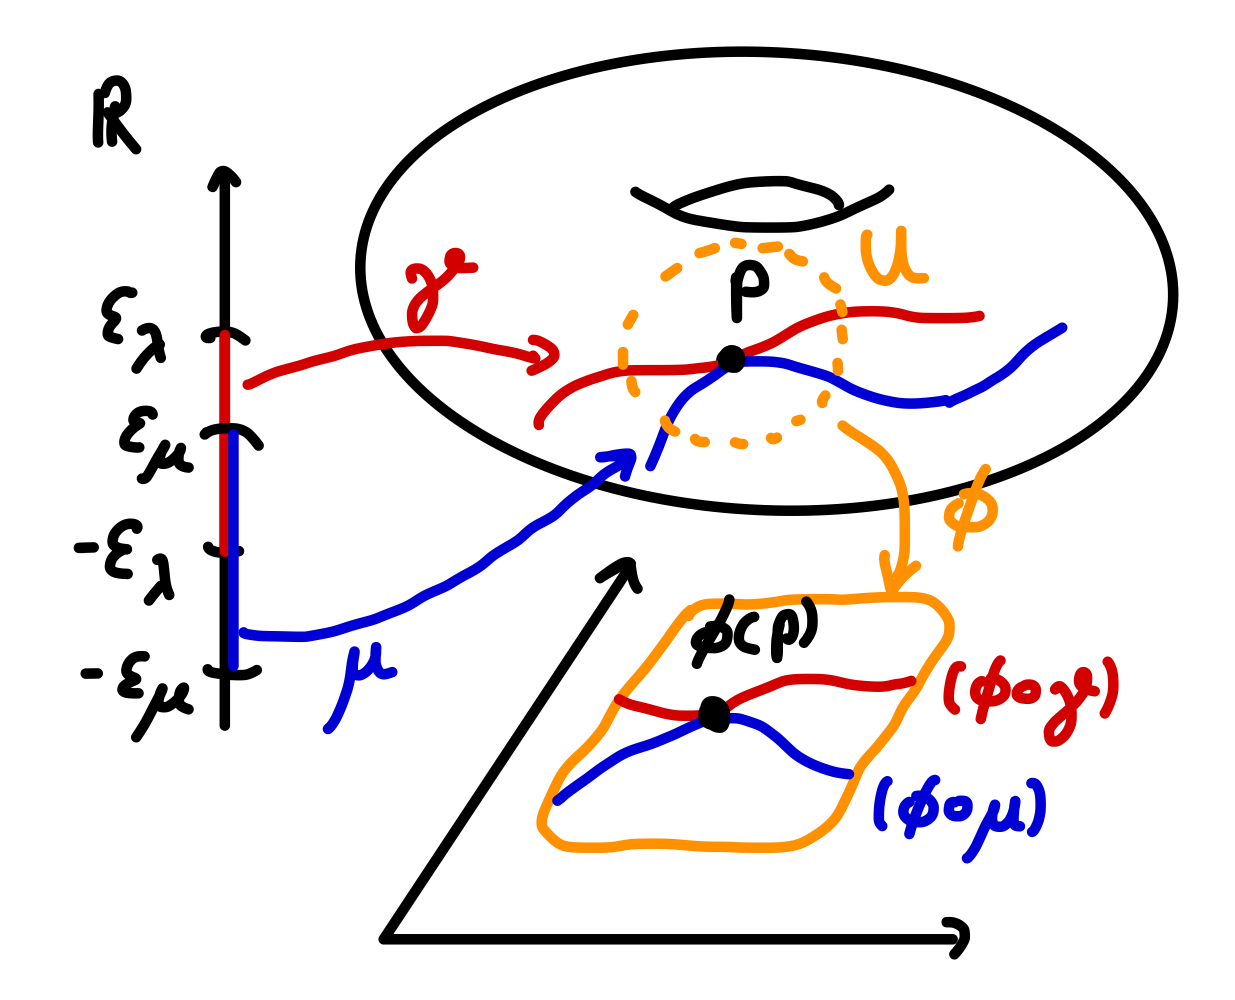
\includegraphics[width=0.2\linewidth]{Bilder/tangentialvek2.png}
\caption{Zwei äquivalente Kurven $\gamma \approx_p \mu$.}
\end{figure}
\end{definition}
Wir entwickeln noch eine dritte Beschreibung.\\
\begin{lemma}{$C^\infty$-Algebra}{}
Sei $C^\infty(M, \R)$ der Vektorraum der glatten Funktionen auf $M$ mit Werten in $\R$. Durch punktweise Multiplikation wird $C^\infty(M, \R)$ zur \textit{Algebra} über $\R$.
\end{lemma}
\begin{definition}{Derivation}{deriv}
Eine \textbf{Derivation} im Punkt $p \in M$ ist eine $\R$-lineare Abbildung
\begin{equation}
\Df: C^\infty(M, \R) \to \R,
\end{equation}
die die \textit{Leibnizregel} $\Df (f \cdot g) = \Df (f) g(p) + f(p) \Df (g)$ erfüllt.\\
Die Menge der Derivationen in $p$ wird mit $\der{p}$ bezeichnet.
\end{definition}
Die Operationen $(\Df_1 + \Df_2)(f) := \Df_1 (f) + \Df_2 (f)$ und $(\alpha \Df)(f) := \alpha \cdot \Df(f)$ machen $\der{p}$ zum reellen VR.
\begin{bemerkung}Konstante Funktionen\\
Für $f(x) \equiv 1$ gilt $f^2 = f$ und damit $\Df (f) = \Df (f^2) = \Df (f) f(p) + f(p) \Df (f)$. Daraus folgt $\Df (f) = 0$. Allgemeiner ist der Wert aller $\Df \in \der{p}$ auf konstanten Funktionen gleich $0$.
\end{bemerkung}
\begin{beispiel}Standardkoordinaten\\
Betrachte $M \sub \R^n$ mit Standardkoordinaten $(x_1, \dots, x_n)$. Die partiellen Ableitungen, ausgewertet in $p \in \R^n$, sind Beispiele für Derivationen in $p$:
\begin{align}
\left.\frac{\partial}{\partial x_i}\right|_p : C^\infty (\R^n, \R) &\to \R \\
f &\mapsto \frac{\partial f}{\partial x_i}(p).
\end{align}
Verallgemeinern lässt sich das wie folgt: Sei $M$ eine glatte MFK und $\phi: U \to V \in \R^k$ eine Karte um $p$ mit Koordinaten $x_i = \pi_i \circ \phi$. Nun definieren wir:
\begin{align}
\left.\frac{\partial}{\partial x_i}\right|_p : C^\infty (M, \R) &\to \R \\
f &\mapsto \frac{\partial (f \circ \phi^{-1})}{\partial x_i}(\phi(p)).
\end{align}
Dies ist eine Derivation in $p \in M$.
\begin{beweis}
Linearität und Leibnizregel sind durch die Ableitungsregeln im $\R^k$ gegeben. Wir zeigen exemplarisch die Leibnizregel:
\begin{align}
\left. \frac{\partial}{\partial x_i}\right|_p (f \cdot g) &= \frac{\partial((f\cdot g)\circ \phi^{-1})}{\partial x_i} (\phi(p)) \\
&= \frac{\partial((f \circ \phi^{-1})( g \circ \phi^{-1}))}{\partial x_i} (\phi(p)) \\
&= \frac{\partial(f \circ \phi^{-1})}{\partial x_i}(\phi(p))\cdot (g \circ \phi^{-1})(\phi (p)) + (f \circ \phi^{-1}) (\phi (p)) \cdot \frac{\partial(g \circ \phi^{-1})}{\partial x_i}(\phi(p)) \\
&=\left.\frac{\partial}{\partial x_i}\right|_p (f) \circ g(p) + f(p) \circ \left.\frac{\partial}{\partial x_i}\right|_p (g)
\end{align}
\end{beweis}
\end{beispiel}
\begin{bemerkung}
Um $\Df \in \der{p}$ auf $f \in C^\infty (M, \R)$ auszuwerten, müssen wir $f$ nur auf einer beliebig kleinen Umgebung von $p$ kennen.
\end{bemerkung}
\begin{satz}{Richtungsableitung}{richtungsabl}
Sei $\phi: U \to V \sub \R^n$ eine Karte um $p \in M$ mit Koordinatenfunktionen $(x_1, \dots, x_n)$. Dann ist die Abbildung 
\begin{align}
T_pM &\to \der{p} \\
[\phi, v] &\mapsto \Df_{[\phi, v]}
\end{align}
mit der Richtungsableitung von $f \circ \phi^{-1}: V \to \R$ in Richtung $v \in T_{\phi(p)}M$, gegeben durch $\Df_{[\phi, v]}(f) = v (f \circ \phi^{-1})$, ein Isomorphismus von $\R$-Vektorräumen.
\begin{figure}[H]
\label{fig:tangentialvek3}
\centering
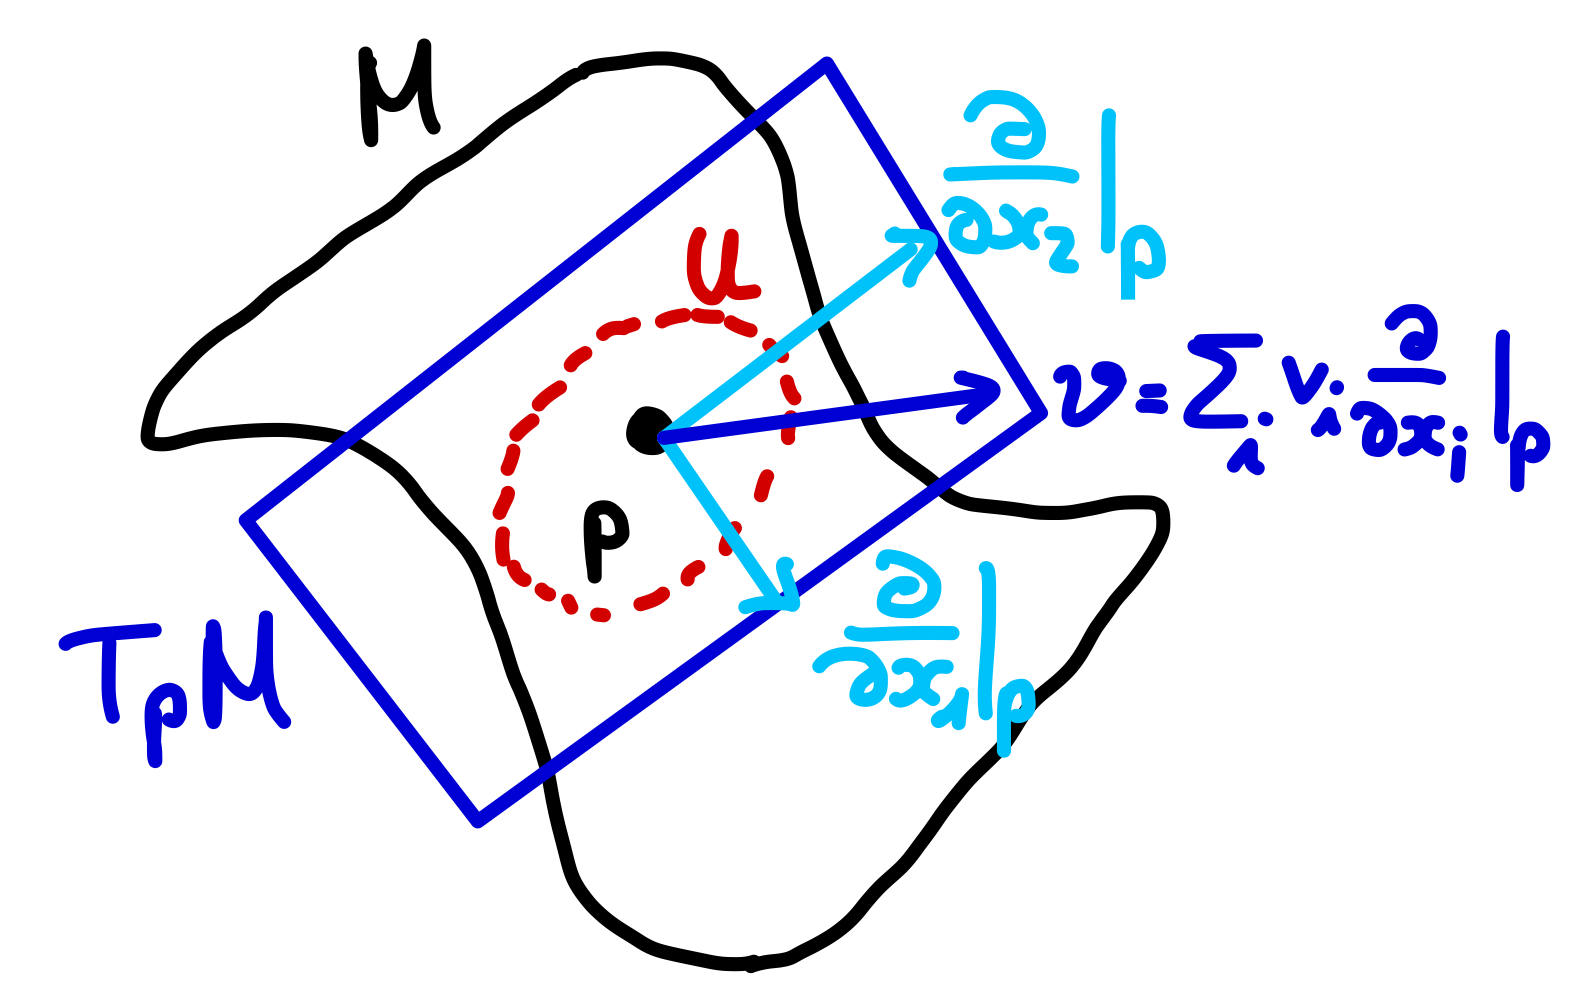
\includegraphics[width=0.2\linewidth]{Bilder/tangentialvek3.png}
\caption{Der von $\frac{\partial}{\partial x_i}$ aufgespannte Tangentialraum an $p$.}
\end{figure}
\end{satz}
\begin{beweis}
Die Abbildung ist durch die Kettenregel wohldefiniert.\\
Der Tangentialvektor $[\phi, (\phi|_p, e_i)]$ wird auf $\left.\frac{\partial}{\partial x_i}\right|_p$ abgebildet. Für die lokal auf $U$ definierten Koordinatenfunktionen $x_j: U \to \R$ gilt aber $\frac{\partial x_j}{\partial x_i} (p) = \delta_{ij}$, also ist die oben definierten Abbildung injektiv. Um zu zeigen, dass sie surjektiv ist, gilt es, zu zeigen, dass\footnote{$\langle \dots \rangle$ steht hier für das Erzeugnis.}
\begin{equation}
\der{p} = \left\langle \left. \frac{\partial}{\partial x_1}\right|_p, \dots, \left. \frac{\partial}{\partial x_n}\right|_p \right\rangle
\end{equation}
\let\qed\relax
\end{beweis}
\begin{lemma}{Taylorentwicklung}{}
Ist $f \in C^\infty (M, \R)$ und $\phi: U \to V \in \R^n$ eine Karte um $p$ mit Koordinaten $(x_1, \dots, x_n)$, dann existiert eine offene Umgebung $W \sub U$ von $p$ und Funktionen $f: W \to \R$, $i \in \{1, \dots, n \}$, sodass $f|_W (q) = f(p) + \Sum{i,1,n} (x_i(q)-x_i(p)) \cdot f_i(q)$.$(\ast)$
\end{lemma}
\begin{beweis}
Sei $W' \sub V = \phi(U)$ eine konvexe Umgebung von $\phi(p)$. Wir schreiben $x_0 := \phi(p)$. Dann gilt für $x \in W'$:
\begin{equation}
(f \circ \phi^{-1})(x)-(f \circ \phi^{-1})(x_0) = \int_0^1 \frac{d}{dt} (f \circ \phi^{-1})(x_0 + t(x-x_0)) dt = \Sum{i,1,n} (x_i - x_i(p)) \underbrace{\int_0^1 \frac{\partial(f \circ \phi^{-1})}{\partial x_i}(x_0 + t(x-x_0))dt}_{=:\tilde{f}_i(x)}
\end{equation}
Mit $W:= \phi^{-1}(W'), q= \phi^{-1}(x)$ und $f_i: W \to \R$, definiert als $\tilde{f}_i \circ \phi$, folgt $(\ast)$. 
\end{beweis}
Weiter mit der Hauptaussage:
\begin{beweis}
Aus $(\ast)$ erhalten wir
\begin{equation}
\left. \frac{\partial}{\partial x_i}\right|_p (f) = \Sum{j,1,n} \left. \frac{\partial}{\partial x_i}\right|_p (x_j - x_j(p)) \cdot f_j] = \Sum{j,1,n} \delta_{ij} \cdot f_j (p) + \cancel{(x_j(p)-x_j(p))} \cdot \left. \frac{\partial}{\partial x_i}\right|_p (f_j) = f_i(p)
\end{equation}
Für eine beliebige Derivation $\Df \in \der{p}$ gilt nun
\begin{equation}
\Df (f) = \Sum{i, 1,n} \Df(x_i - x_i (p)) \cdot f_i = \Sum{i,1,n} \Df(x_i) \cdot f_i(p)+\cancel{(x_i(p)-x_i(p))} \cdot \Df (f_i) = \left( \Sum{i,1,n} \Df (x_i) \left.\frac{\partial}{\partial x_i}\right|_p \right)(f)
\end{equation}
Wir haben also ein beliebiges $\Df \in \der{p}$ als Linearkombination der $\left.\frac{\partial}{\partial x_i}\right|_p$ ausgedrückt.
\end{beweis}
\begin{warning}
Ab jetzt schreiben wir nur $v \in T_pM$ für einen Tangentialvektor in $p \in M$.
\end{warning}
\begin{definition}{Differential}{diff}
Seien $M,N$ glatte MFK und $F: M \to M$ eine glatte Abbildung zwischen diesen. Das \textbf{Differential} oder der \textbf{Pushforward} von $F$ im Punkt $p \in M$ ist die lineare Abbildung:
\begin{align}
F_{\ast, p}: T_pM &\to T_{F(p)}N \\
v &\mapsto F_{\ast, p} (v)
\end{align}
mit $F_{\ast, p} (v)(f) = v(f \circ F)$ für alle $f \in C^\infty (N, \R)$.
\begin{figure}[H]
\label{fig:differential}
\centering
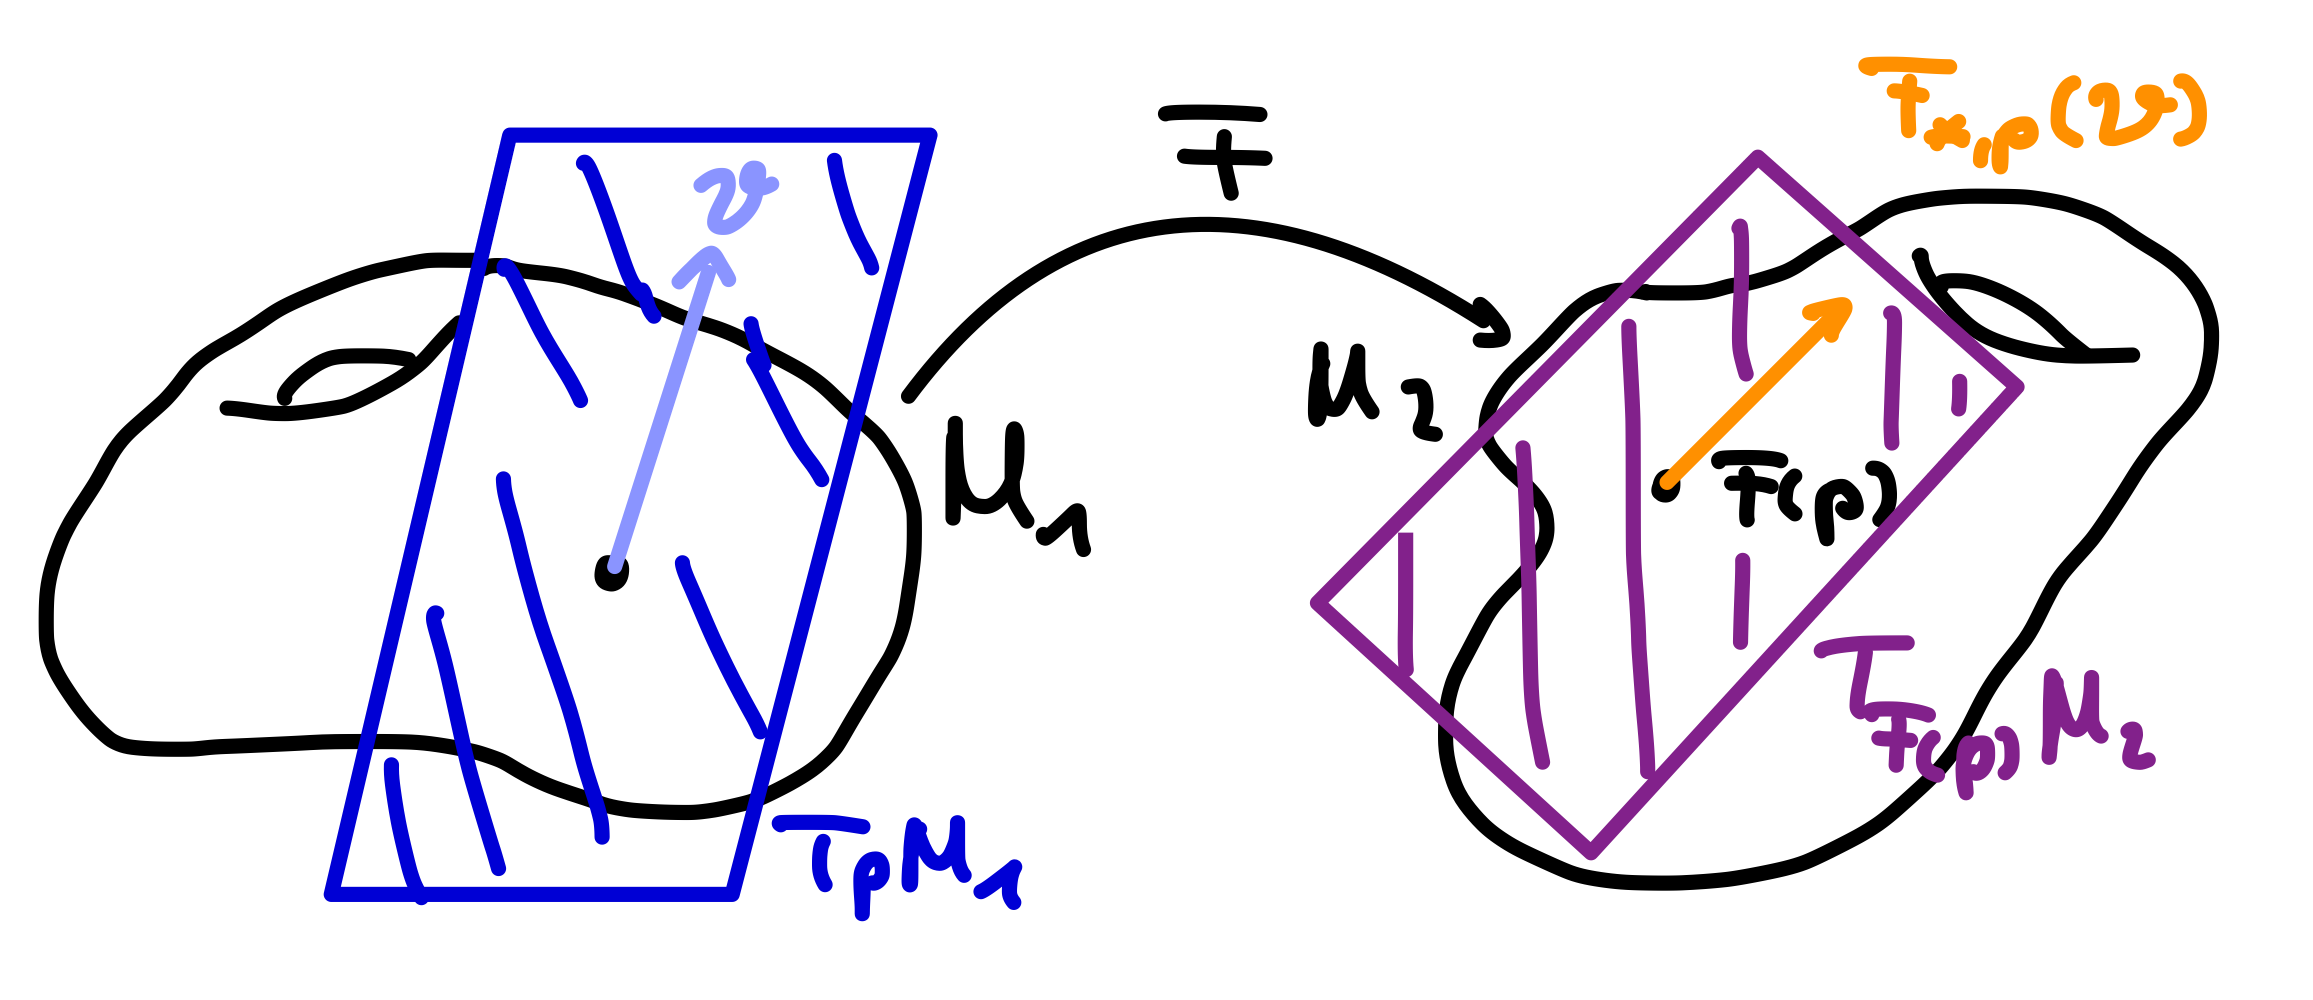
\includegraphics[width=0.3\linewidth]{Bilder/differential.png}
\caption{Dargestellt ist das Differential einer glatten Abbildung $F: M_1 \to M_2$.}
\end{figure}
\end{definition}
\begin{definition}{\textit{lokaler Diffeomorphismus}}{lokalerdiff}
Seien $M,N$ glatte MFKn mit oder ohne Rand. Dann heißt $F: M \to N$ \textbf{lokaler Diffeomorphismus}, wenn alle $p \in M$ eine Umgebung $U \sub M$ haben, sodass $F(U)$ offen in $N$ und $F|_U: U \to F(U)$ ein Diffeomorphismus ist.
\end{definition}
\begin{theorem}{\textit{Umkehrsatz für Mannigfaltigkeiten}}{großerumkehrsatz}
Seien $M,N$ glatte MFKn und sei $F:M \to N$ eine glatte Abbildung. Wenn $F_{\ast, p}$ invertierbar ist in $p \in M$, so existieren zusammenhängende Umgebungen $U_0$ von $p$ und $V_0$ von $F(p)$, sodass
\begin{equation}
F|_{U_0}: U_0 \to V_0
\end{equation}
ein Diffeomorphismus ist.
\end{theorem}
Es gelten die üblichen Rechenregeln, unter anderem die Kettenregel:
\begin{satz}{Kettenregel}{kettenrgl}
Sind $F: M_1 \to M_2$ und $G: M_2 \to M_3$ glatt, so gilt
\begin{equation}
(G \circ F)_{\ast, p} = G_{\ast, F(p)} \circ F_{\ast, p}.
\end{equation}
\end{satz}
\begin{beweis}
Für $f: M_3 \to \R$ gilt 
\begin{equation}
G_{\ast, F(p)} \circ F_{\ast, p} (v)(f) = F_{\ast, p} (v) (f \circ G) = v(f \circ (G \circ F)) = (G \circ F)_{\ast, p} (v)(f).
\end{equation}
\end{beweis}
Für konkrete Rechnungen wollen wir $F_{\ast, p}$ in Koordinaten ausdrücken:\\
Sei dazu $F: M_1 \to M_2$ glatt und $p \in M_1$. Sei $\phi: U \to \R^n$ eine Karte um $p$ mit Koordinaten $(x_1, \dots, x_n)$ und $\psi: W \to \R^m$ eine eine Karte um $F(p)$ mit Koordinaten $(y_1, \dots, y_m)$. Für $w \in T_{F(p)}M_2$ und $f \in C^\infty(M_2)$ gilt dann 
\begin{equation}
w(f) = \Sum{j,1,m} w(y_j) \left.\frac{\partial}{\partial y_j}\right|_{F(p)}(f).
\end{equation} 
Daraus folgt für $v \in T_pM_1$:
\begin{equation}
F_{\ast, p}(v)(f) = \Sum{j,1,m}F_{\ast, p}(v)(y_j) \left.\frac{\partial}{\partial y_j}\right|_{F(p)}(f) = \Sum{j,1,m} v(y_j \circ F) \left.\frac{\partial}{\partial y_j}\right|_{F(p)}(f).
\end{equation}
Die Darstellung $v = \Sum{i,1,n} v_i \left.\frac{\partial}{\partial x_i}\right|_{p}$ liefert
\begin{equation}
F_{\ast, p}(v)(f) = \Sum{i,1,n}\Sum{j,1,m} \frac{\partial (y_i \circ F \circ \phi^{-1})}{\partial x_i} (\phi(p)) \cdot v_i \cdot \left.\frac{\partial}{\partial y_j}\right|_{F(p)}(f).
\end{equation}
Das ist auch gleich der Beweis für:
\begin{satz}{Matrixdarstellung}{mtrx}
In den lokalen Koordinaten $\phi: U \to \R^n$ auf $M_1$ und $\psi: W \to \R^m$ auf $M_2$ hat $F_{\ast, p}: T_pM_1 \to T_{F(p)}M_2$ bezüglich der Basen $\left( \left.\frac{\partial}{\partial x_1}\right|_p, \dots, \left.\frac{\partial}{\partial x_n}\right|_p \right)$ von $T_pM_1$ und $\left( \left.\frac{\partial}{\partial x_1}\right|_{F(p)}, \dots, \left.\frac{\partial}{\partial x_m}\right|_{F(p)} \right)$ von $T_{F(p)}M_2$ die Matrixdarstellung
\begin{equation}
\left\{ \frac{\partial (\psi \circ F \circ \phi^{-1})_j}{\partial x_i} (\phi(p))\right\}_{\substack{j \in \{1, \dots, m\}\\i \in \{ 1, \dots, n\}}}.
\end{equation}
\end{satz}
\begin{beispiel}
Sei $c: (a,b) \to M$ eine glatte Kurve in $M$. Für $t_0 \in (a,b)$ bezeichnet $\left.\frac{\partial}{\partial t}\right|_{t_0}$ den Standard-Basisvektor von $T_{t_0}\R \cong \R$. Der Tangentialvektor an $c$ in $c(t_0)$ ist dann $c'(t_0)=\dot{c}(t_0):= c_{\ast, t_0}\left(\left.\frac{\partial}{\partial t}\right|_{t_0} \right) \in T_{c(t_0)}M$. Ist $F: M \to N$ eine glatte Abbildung, gilt $F_{\ast, c(t_0)} (c'(t_0)) = (F \circ c)'(t_0) \cdot \left.\frac{\partial}{\partial t}\right|_{F \circ c(t_0)}$.
\end{beispiel}
\begin{definition}{Submersion, Immersion, Einbettung}{subimein}
Eine glatte Abbildung $F: M \to N$ zwischen glatten MFK $M, N$ heißt:
\begin{itemize}
\item \textbf{Immersion}, wenn $F_{\ast, p}: T_pM \to T_{F(p)}N$ für alle $p \in M$ injektiv ist.
\item \textbf{Submersion}, wenn $F_{\ast, p}: T_pM \to T_{F(p)}N$ für alle $p \in M$ surjektiv ist.
\item \textbf{Einbettung}, falls $F$ eine Immersion ist und $F: M \to F(M) \sub N$ ein \textit{Homöomorphismus} ist.
\end{itemize}
\end{definition}
\begin{bemerkung}
Einbettung $\implies$ injektive Immersion, aber injektive Immersion $\xcancel{\implies}$ Einbettung.
\end{bemerkung}
\begin{beispiele} Submersionen, Immersionen und Einbettungen\\
\begin{enumerate}
\item Wir betrachten $F: \R \to \R^2, F(t):=(\sin t, \sin 2t)$. Man rechnet nach, dass $F$ eine Immersion ist. Auf $(0, 2\pi)$ ist $F$ auch injektiv, aber keine Einbettung. Auf $(\epsilon, 2\pi - \epsilon)$ für $\epsilon > 0$ ist $F$ aber eine Einbettung.
\item Sei $M=\Z$ und $N= \sph^1 \cong \quotient{\R}{\Z}$. Für $\alpha \in \R, \Q$ ist die Abbildung $F_\alpha: \Z \to \sph^1, \ k \mapsto k \alpha \mod 1$ eine injektive Immersion, aber keine Einbettung, da $F_\alpha(\Z) \sub \sph^1$ nicht die diskrete Topologie hat.
\item Jede Projektion $\pi: \R^n \to L \sub \R^k$ auf einen linearen UR $L \in \R^n$ entlang des orthogonalen Komplements $L^\perp \sub \R^n$ ist eine Submersion. Jede lineare Einbettung $A: \R^k \to \R^n$ ist eine Immersion.
\item $F: \R^{n+1} \exc \{0\}  \to \R, \ F(x) := ||x||^2$ ist eine Submersion, denn $\Ds F_x(v) = 2 \ip{x,v}$.
\item $G:  \R^{n+1} \exc \{0\} \to \sph^n, \ G(x):=\frac{x}{||x||}$ ist auch eine Submersion.
\end{enumerate}
\end{beispiele}
\begin{satz}{\textit{Rangsatz}}{rangsatz}
Seien $M$ und $N$ glatte MFKn mit $m = \dim M$ und $n = \dim N$. Sei weiterhin $F: M \to N$ glatt mit konstantem Rang $r$. Dann existieren für jedes $p \in M$ glatte Karten $(U,\phi)$ von $M$ um $p$ und $(V,\psi)$ von $N$ um $F(p)$, sodass $F(U) \sub V$, in denen $F$ die lokale Koordinatendarstellung 
\begin{equation}
\hat{F} (x_1, \dots, x_r, x_{r+1}, \dots, x_m) = (x_1, \dots, x_r, 0, \dots, 0)
\end{equation}
besitzt.\\
Ist $F$ eine glatte \textcolor{red}{Submersion}, so gilt sogar
\begin{equation}
\hat{F} (x_1, \dots, x_n, x_{n+1}, \dots, x_m) = (x_1, \dots, x_n).
\end{equation}
Ist $F$ eine glatte \textcolor{red}{Immersion}, so gilt hingegen
\begin{equation}
\hat{F} (x_1, \dots, x_m) = (x_1, \dots, x_m, 0, \dots, 0).
\end{equation}
\begin{figure}[H]
\label{fig:submersionimmersion}
\centering
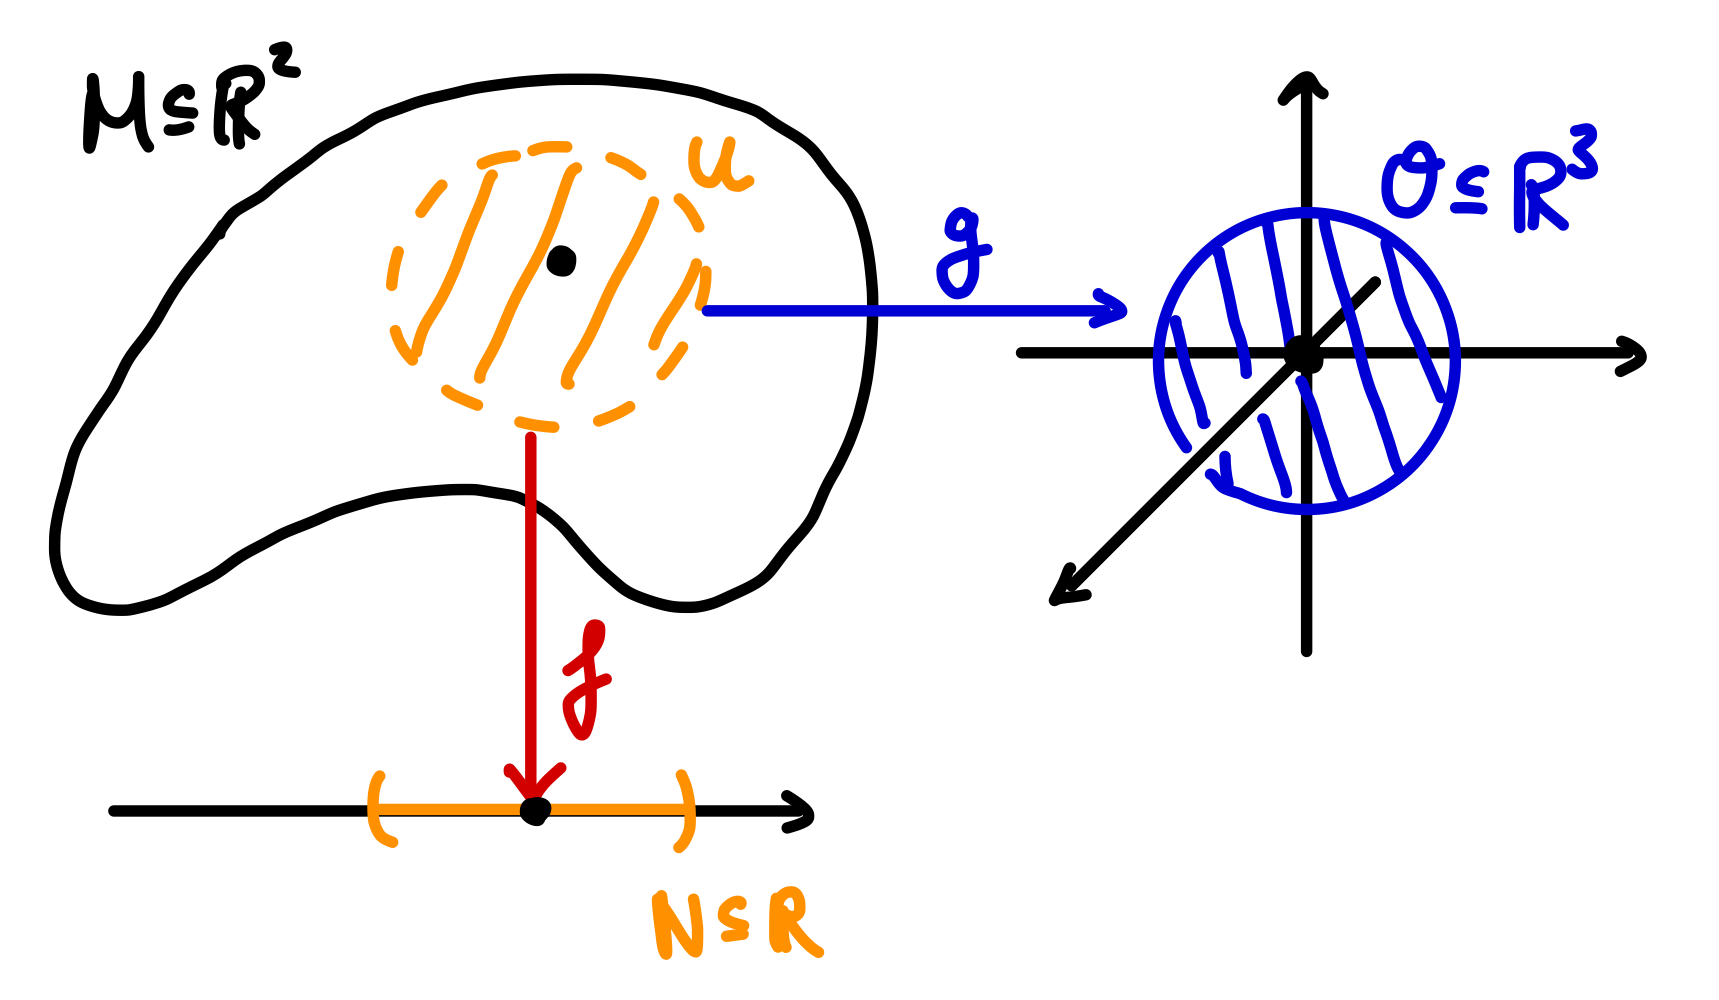
\includegraphics[width=0.3\linewidth]{Bilder/submerimmer.png}
\caption{Lokal sieht eine Submersion $f$ wie eine kanonische Projektion und eine Immersion $g$ wie eine kanonische Injektion aus.}
\end{figure}
\end{satz}
\begin{definition}{Untermannigfaltigkeiten reloaded}{Umfneu}
Seien $N, M$ glatte MFKn. Eine Teilmenge $S \sub M$ heißt \textbf{Untermannigfaltigkeit (UMF)}, falls $S$ das Bild einer Einbettung $f: N \to M$ ist.
\end{definition}
\begin{bemerkung}
Äquivalent ist die Beschreibung von UMF als Teilmengen $U \sub M$ einer MFK $M$, die lokal Urbild eines Punktes unter einer lokal definierten Submersion sind.
\end{bemerkung}
Für $M=\R^n$ erhalten wir wieder unser schon bekanntes Konzept aus \ref{umfn}.
\begin{definition}{Regularität}{reg}
Sei $F: M \to N$ eine glatte Abbildung.\\
Ein Punkt $p \in M$ heißt \textbf{regulär für} $F$, falls $F_{\ast, p}: T_pM \to T_{F(p)}N$ surjektiv ist. Andernfalls heißt $p$ \textbf{kritisch} für $F$.\\
Ein Punkt $q \in N$ heißt \textbf{regulärer Wert von} $F$, falls $F^{-1}(q)$ nur aus regulären Punkten besteht. Wenn $F^{-1}(q)$ mindestens einen kritischen Punkt enthält, heißt $q \in N$ \textbf{kritischer Wert}.
\end{definition}
\begin{satz}{Satz vom regulären Wert}{regwertsatz}
Sei $F: M \to N$ eine glatte Abbildung und $q \in N$ ein regulärer Wert von $F$.\\
Dann ist $F^{-1}(q) \sub M$ eine glatte UMF von $M$ der Dimension $\dim M - \dim N$. Für $p \in F^{-1}(q)$ gilt außerdem $T_pF^{-1} (q) = \ker F_{\ast, p}$.
\begin{figure}[H]
\label{fig:regulaer}
\centering
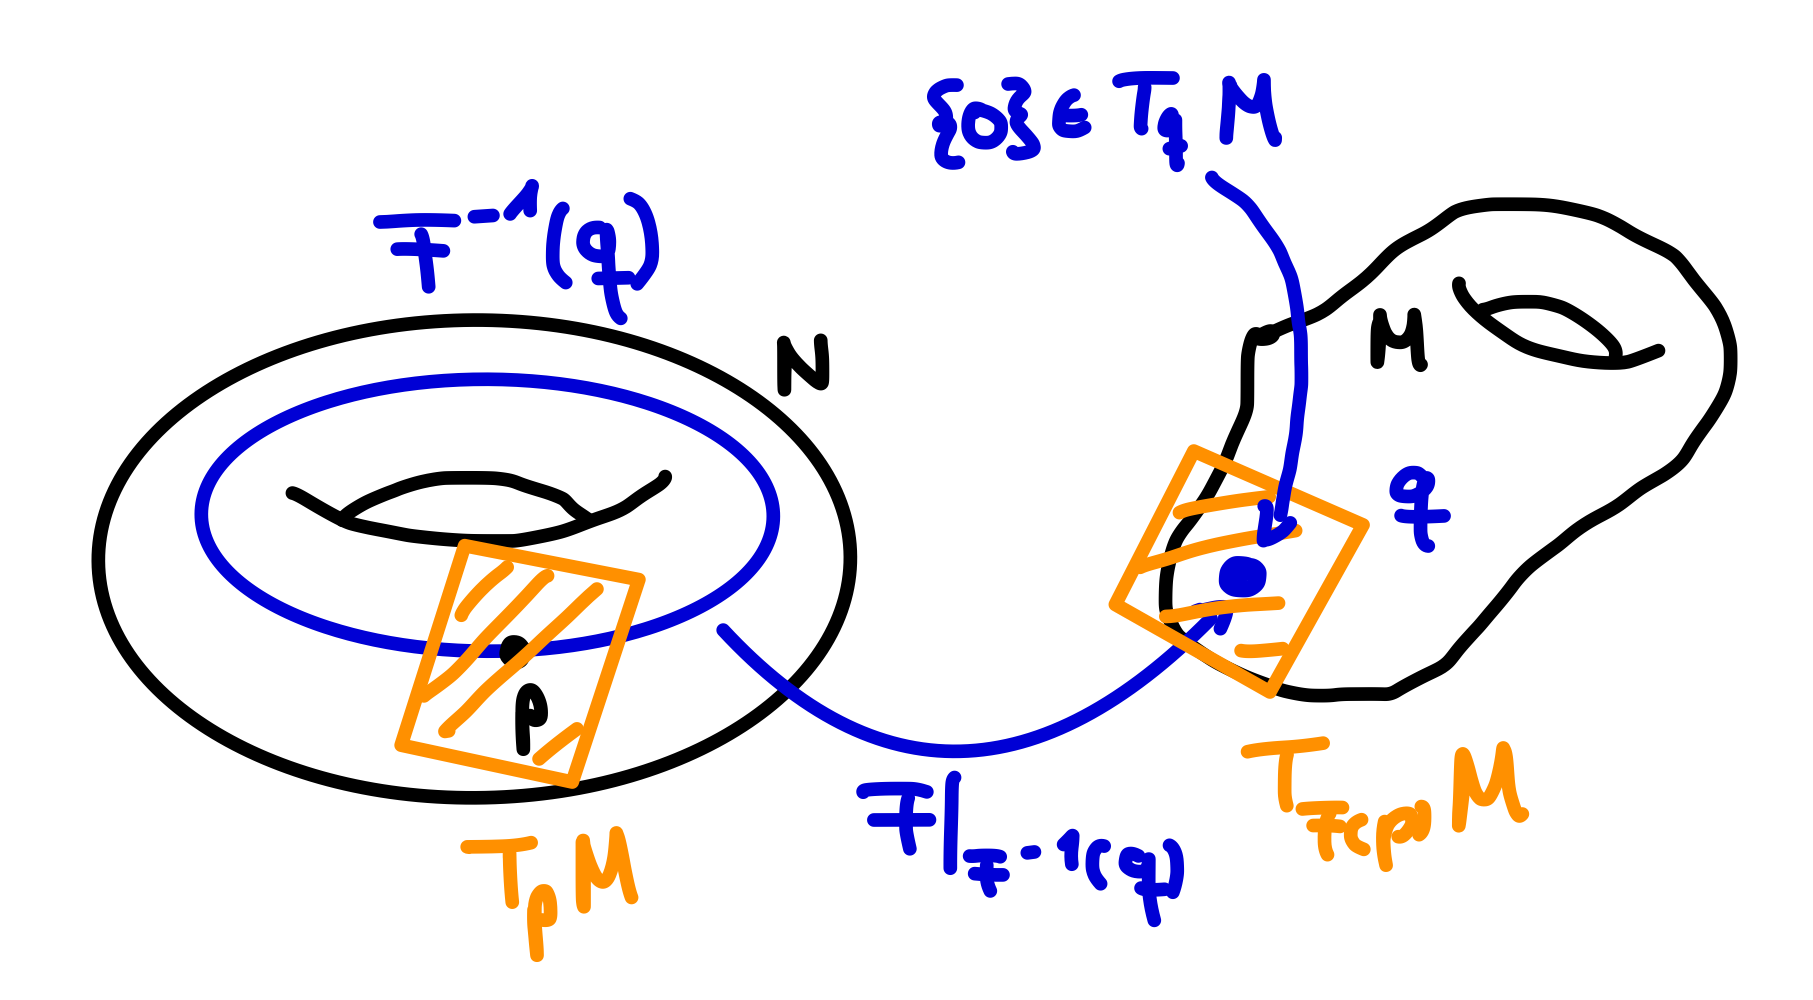
\includegraphics[width=0.3\linewidth]{Bilder/regulaer.png}
\caption{Das Urbild von $q$ unter $F$ sind die Niveaulinien von $F$, die eine UMF von $M$ darstellen.}
\end{figure}
\end{satz}
\begin{bemerkung}
Für $M = \R^n$ und $N= \R^k$ erhalten wir eine unserer äquivalenten Charakterisierungen von UMFn. Der allgemeine Fall folgt aus dem Spezialfall, indem man mit lokalen Karten arbeitet. Die Nützlichkeit des Satzes ergibt sich aus folgendem Satz.
\end{bemerkung}
\begin{satz}{Satz von Sard}{sard}
Sei $F: M \to N$ eine glatte Abbildung.\\
Dann hat die Menge der kritischen Werte von $F$ Lebesgue-Maß $0$ in $N$, die Menge der regulären Werte ist also dicht.
\end{satz}
\begin{bemerkung}
$A \sub N$ hat Lebesgue-Maß $0$, falls für jede Karte $\phi: U \to V \sub \R^k$ die Menge $\phi(A \cap U) \sub \R^k$ Lebesgue-Maß $0$ hat.
\end{bemerkung}
\begin{definition}{\textit{Transversalität}}{transvers}
Seien $M,N$ glatte MFKn und $F: M \to N$ glatt. Sei $S \sub N$ eine UMF. $F$ heißt \textbf{transvers} zu $S$, falls in allen $p \in M$ mit $F(p) \in S$ gilt:
\begin{equation}
F_{\ast, p} (T_pM) + T_{F(p)}S=T_{F(p)}N.
\end{equation}
\end{definition}
\begin{satz}{\textit{UMF als Urbilder transverser Abbildungen}}{transversumf}
Ist $F$ transvers zu $S$, so ist $F^{-1} \sub M$ eine UMF mit Dimension
\begin{equation}
\dim F^{-1} = \dim M + \dim S - \dim N.
\end{equation}
\end{satz}
\begin{beweis}
Übung (A8)
\end{beweis}
\begin{satz}{\textit{Einbettungen als injektive Immersionen}}{injektiveinbettung}
Seien $M,N$ glatte MFKn und sei $M$ darüber hinaus kompakt. Sei weiterhin $F: M \to N$ eine \textcolor{red}{injektive Immersion}. Dann ist $F$ eine Einbettung.\\
Gilt $\dim M = \dim N$ und ist $N$ zusammenhängend, so ist $F$ ein Diffeomorphismus.
\end{satz}
\begin{beweis}
Übung (A10)
\end{beweis}

\section{Vektorbündel, Lie-Gruppen und Integration auf Mannigfaltigkeiten}
\subsection{Vektorbündel und Integralkurven}
\label{subsec:tangentialbündel}
Jetzt wollen wir $TM := \bigcup_{x \in M} T_xM$ die Struktur einer glatten MFK geben, damit $\pi: TM \to M$ glatt ist und weitere nützliche Eigenschaften aufweist.
\begin{definition}{Vektorbündel}{vekbund}
Ein \textbf{Vektorbündel vom Rang} $k$ \textbf{über einer MFK} $B$ ist ein Tripel $(E, p, B)$, wobei $E$ und $B$ glatte MFK sind und $p: E \to B$ eine \textit{surjektive Submersion} mit folgenden Eigenschaften ist:
\begin{itemize}
\item Für jedes $b \in B$ hat $p^{-1}(b)$ die Struktur eines reellen Vektorraums der Dimension $k$.
\item Für jedes $b \in B$ existiert eine offene Umgebung $U \sub B$ von $b$ und ein Diffeomorphismus $\phi: p^{-1}(U) \to U \times \R^k$, sodass das Diagramm
\begin{center}
\begin{tikzcd}
    p^{-1}(U) \arrow[r,"\phi"] \arrow[d,"p"] & U \times \R^k \arrow[dl,"pr_U"] \\
    U
\end{tikzcd}
\end{center}
kommutiert und $\phi|_{p^{-1}(b)}:p^{-1}(b) \to \{b\} \times \R^k$ ein  linearer Isomorphismus ist.
\end{itemize}
Dann heißt $E$ \textbf{Totalraum} des Bündels, $B$ die \textbf{Basis} und die Abbildungen $\phi: p^{-1}(U) \to U \times \R^k$ \textbf{lokale Trivialisierungen}. Das Urbild $p^{-1}(b)$ heißt \textbf{Faser von} $p$ über $b$.
\begin{figure}[H]
\label{fig:vektorbuendel}
\centering
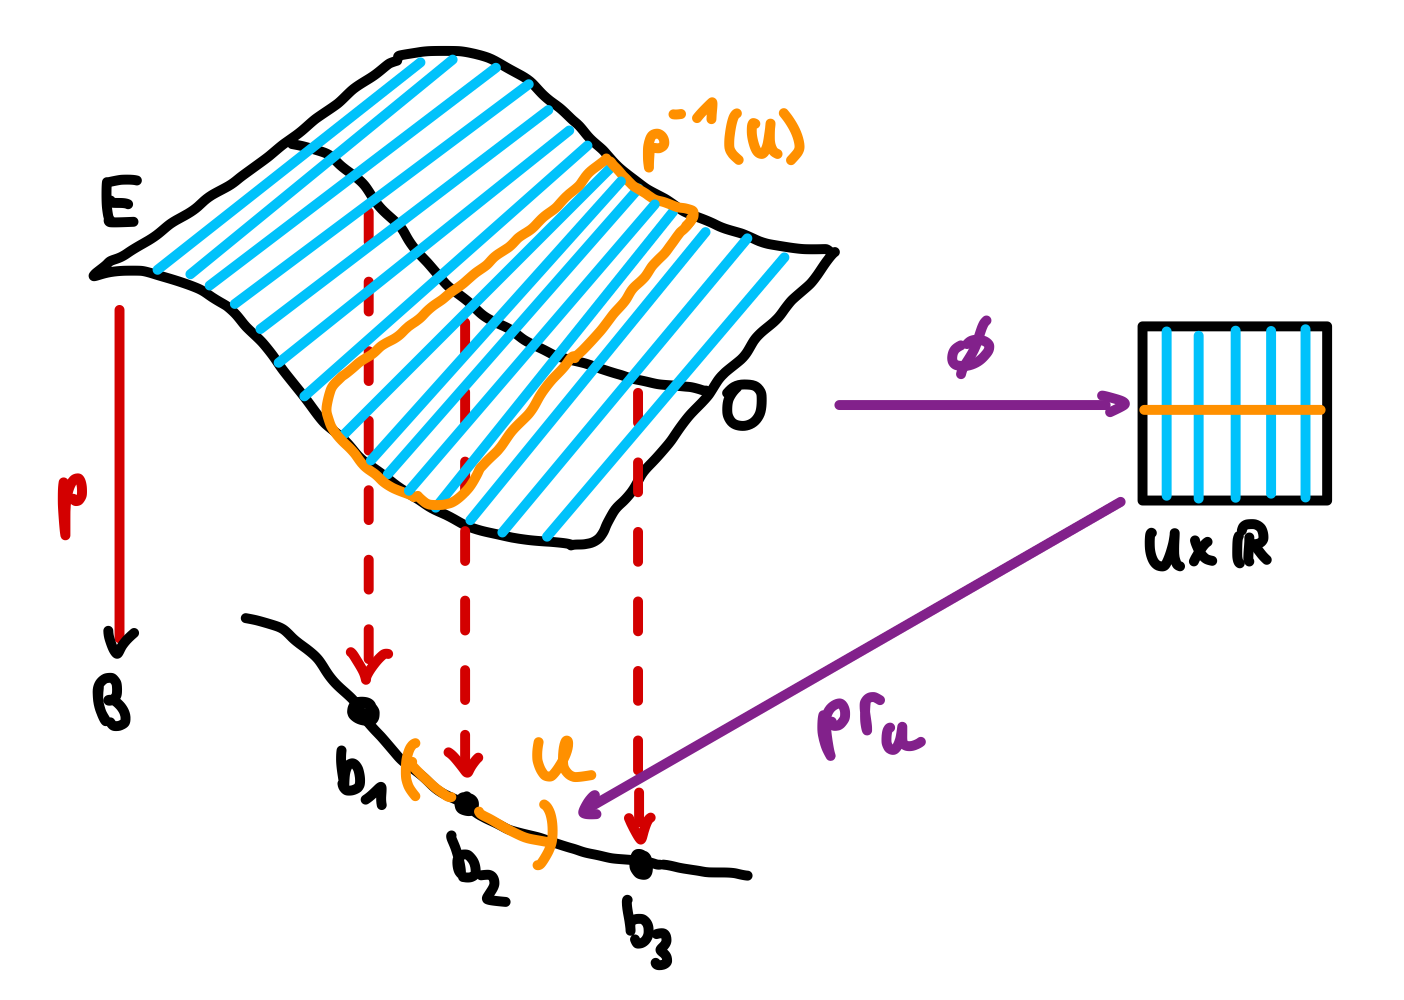
\includegraphics[width=0.3\linewidth]{Bilder/vektorbuendel.png}
\caption{Ein Vektorbündel.}
\end{figure}
\end{definition}
\begin{beispiele}Vektorbündel\\
\begin{enumerate}
\item Über jeder MFK $M$ gibt es das \textit{triviale Vektorbündel} von Rang $k$, gegeben durch
\begin{center}
\begin{tikzcd}
M \times \R^k \arrow[r, "p"] & M
\end{tikzcd}
\end{center}
mit $p(x, y) =x$.
\item Wir erinnern uns an die Definition vom $\R P^n$ als Raum der $1$-dim linearen UR im $\R^{n+1}$ und betrachten $E:= \{ (l, v) | l \in \R P^n, v \in l \} \sub \R P^n \times \R^{n+1}$. Mit der offensichtlichen Projektion $p: E \to  \R P^n$ ist $E$ ein Vektorbündel von Rang $1$ über $\R P^n$.
\begin{beweis}
Zuerst gilt es zu zeigen, dass $E \sub \R P^n \times \R^{n+1}$ eine UMF ist. Für den $\R P^n$ haben wir bereits Karten $U_i = \{ l \in \R P^n | \text{Projektion auf} \ i \text{-te Koordinate ist bijektiv}\}$ etabliert. $U_i$ wird parametrisiert durch die Abbildung $\psi_i : \R^n \to \R P^n, \ (x_1, \dots, x_n) \mapsto [(x_1, \dots, x_{i-1}, 1, x_i, \dots, x_n)]$. Das Urbild $p^{-1}(U_i)$ kann parametrisiert werden durch
\begin{align}
\rho_i: \R^n \times \R &\to \R P^n \times \R^{n+1} \\
(x, \lambda) &\mapsto \left( [(x_1, \dots, x_{i-1}, 1, x_i, \dots, x_n)], \lambda \cdot (x_1, \dots, x_{i-1}, 1, x_i, \dots, x_n)\right)
\end{align}
Das ist offenbar eine glatte Immersion, die $p^{-1}(U_i)=E \cap (U_i \times \R^{n+1})$ parametrisiert.
Aus dieser Karte für $E$ erhalten wir die lokalen Trivialisierungen über $U_i$:\\
$\phi_i: p^{-1}(U_i) \to U_i \times \R$ ist gegeben durch $(l, v) \mapsto (\psi_i \times \id_\R) \rho_i^{-1}(l,v)$.
\end{beweis}
\item Tangentialbündel einer UMF $M \sub \R^n$:\\
Mit unseren Konventionen ist $T_xM \sub \{x\} \times \R^n$ ein linearer UR der Dimension $k$. Damit ist dann $TM := \bigcup_{x \in M} T_xM$ eine Teilmenge von $M \times \R^n \sub \R^n \times \R^n$. Um Einzusehen, dass $TM \sub \R^n \times \R^n$ eine UMF ist, benutzen wir die Definition einer UMF als lokales Urbild einer Submersion.
\begin{beweis}
Sei $x\in M$ und sei $\psi: U \to \R^{n-k}$ eine auf einer offenen Umgebung $U$ von $x$ definierte Submersion mit $U \cap M = \psi^{-1}(0)$. Dann gilt für $y \in U \cap M$, dass $T_y M = \ker \psi_{\ast,y}$. Wir können also $TM \cap \left( (U \cap M) \times \R^n \right)$ beschreiben als Urbild von $0 \in \R^{n-k} \times \R^{n-k}$ unter der Abbildung:
\begin{align}
\Psi: U \times \R^n &\to \R^{n-k} \times \R^{n-k}\\
(z, v) &\mapsto \left( \psi(z), (\diff \psi)_z(v) \right).
\end{align}
Das Differential hat Blockform:
\begin{equation}
\diff \Psi_{(z,v)} = \mat{\diff \psi_z, 0}{\ast, \diff \psi_z},
\end{equation}
ist also surjektiv für alle $(z, v) \in U \times \R^n$. Weiterhin gilt
\begin{equation}
\Psi(z,v) = 0 \iff z \in M \wedge v \in T_zM,
\end{equation}
also allgemein $(z, v) \in TM \cap (U \times \R^n)$. Damit ist bewiesen, dass $TM \sub \R^n \times \R^n$ eine UMF der Dimension $2k$ ist.
\end{beweis}
Die Projektion $\pi: TM \to M$ ist als Einschränkung von $\R^n \times \R^n \to \R^n$ glatt, lokale Trivialisierungen erhält man aus der Beschreibung von $M$ über lokale Karten.
\end{enumerate}
\end{beispiele}
\begin{definition}{\textit{direkte Summe}}{direktesumme}
Seien $p_1: E_1 \to B$ und $p_2: E_2 \to B$ zwei Vektorbündel über der MFK $B$. Sei weiterhin $E:=p^{-1}(\Delta)\sub E_1 \times E_2$ das Urbild der Diagonalen $B \cong \Delta := \{(b,b)\ | \ b \in B \} \sub B \times B$. Dann heißt $E = E_1 \oplus E_2$ \textbf{direkte Summe} oder \textbf{Whitney-Summe} der Vektorbündel $E_1$ und $E_2$.\\ 
$(E,p,B)$ ist ein Vektorbündel über $B$ mit $p(e_1, e_2):=p_1(e_1)=p_2(e_2)$.
\end{definition}
\begin{bemerkung}Kozykelbedingung\\
Sei $p: E \to B$ ein Vektorbündel von Rang $k$ und seien $\phi: p^{-1}(U) \to U \times \R^k$ und $\psi: p^{-1}(V) \to V \times \R^k$ zwei lokale Trivialisierungen mit $U \cap V \neq \emptyset$.\\
Dann erhalten wir eine Übergangsabbildung
\begin{align}
\psi \circ \phi^{-1}: (U \cap V) \times \R^k &\to (U \cap V) \times \R^k \\
(b, v) &\mapsto (b, A_b(v)), \ A_b \in \text{GL}(k, \R).
\end{align}
Da $\psi \circ \phi^{-1}$ ein Diffeomorphismus, also insbesondere glatt, ist, ist auch $U \cap V \to \gl{k}{\R}, \ b \mapsto A_b$ glatt. Haben wir nun noch eine dritte Trivialisierung $\rho: p^{-1} (W) \to W \times \R^k$, so erhalten wir Übergangsabbildungen
\begin{align}
\rho \circ \psi^{-1}: (W \cap V) \times \R^k &\to (W \cap V) \times \R^k \\
(b, v) &\mapsto (b, B_b(v)) \\
\rho \circ \phi^{-1}: (W \cap U) \times \R^k &\to (W \cap U) \times \R^k \\
(b, v) &\mapsto (b, C_b(v))
\end{align}
für geeignete Abbildungen $B: W \cap V \to \gl{k}{\R}$ und $C: W \cap U \to \gl{k}{\R}$. Auf $U \cap V \cap W$ gilt $\rho \circ \phi^{-1} = (\rho \circ \psi^{-1})(\psi \circ \phi^{-1})$. Dadurch erhalten wir für $b \in U \cap V \cap W$ die \textbf{Kozykelbedingung}
\begin{equation}
C_b = B_b \circ A_b.
\end{equation}
\begin{figure}[H]
\label{fig:vektorbuendel}
\centering
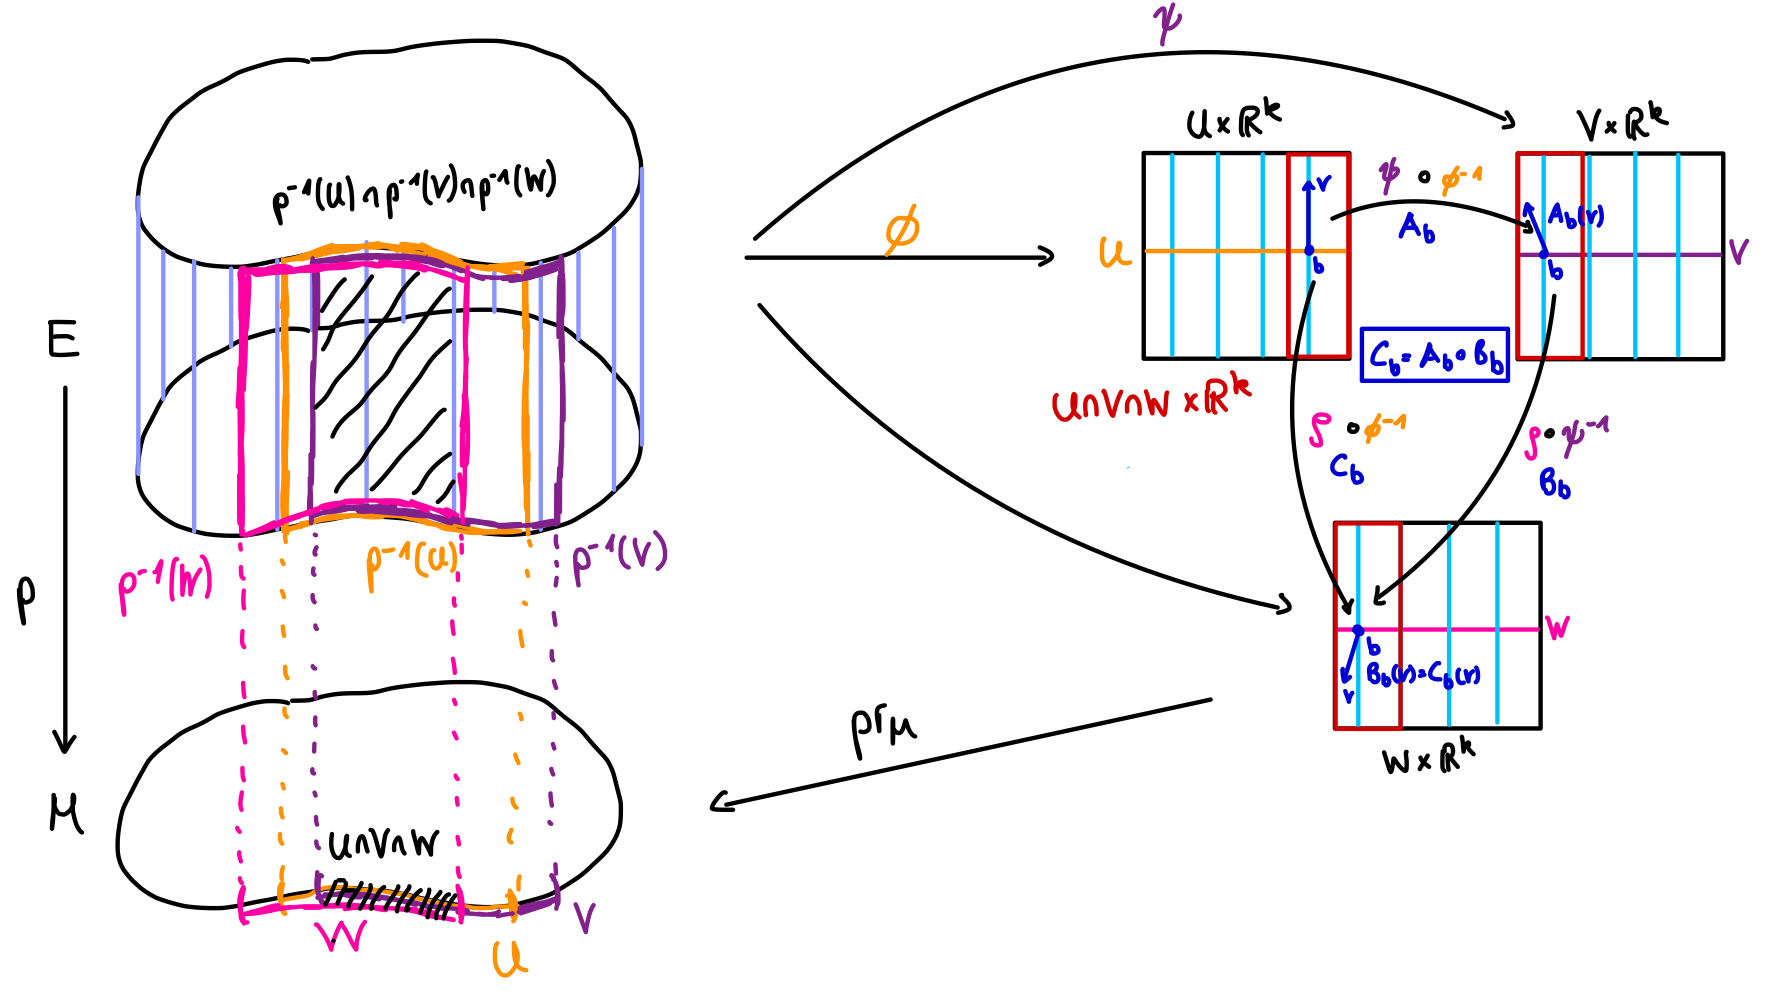
\includegraphics[width=0.5\linewidth]{Bilder/kozykel.png}
\caption{Eine Veranschaulichung der Kozykelbedingung für drei überlappende lokale Trivialisierungen.}
\end{figure}
Umgekehrt gilt Folgendes für die Konstruktion von Vektorbündeln:\\
Sei $B$ eine glatte MFK und $\{ U_\alpha \}_{\alpha  \in I}$ eine offene Überdeckung. Wir nehmen an, dass zu $\alpha, \beta \in I$ Abbildungen $\phi_{\alpha \beta}: U_\alpha \cap U_\beta \to \gl{k}{\R}$ gegeben sind, sodass für $\alpha, \beta, \gamma \in I$ die Kozykelbedingung
\begin{equation}
\left. \phi_{\alpha \gamma} \right|_{U_\alpha \cap U_\beta \cap U_\gamma} = \left. \left(\phi_{\alpha \beta} \circ \psi_{\beta \gamma} \right) \right|_{U_\alpha \cap U_\beta \cap U_\gamma}
\end{equation}
erfüllt ist. Aus diesen Daten konstruieren wir wie folgt ein Vektorbündel von Rang $k$ über $B$:\\
Auf $\amalg_{\alpha \in I} U_\alpha \times \R^k$ definieren wir eine Äquivalenzrelation durch $(x. v) \in U_\alpha \times \R^k \sim (x, w) \in U_\beta \times \R^k$ genau dann, wenn $\phi_{\alpha \beta}(w)=v$. Die Kozykelbedingung garantiert die Transitivität. Sei $E$ die Menge der Äquivalenzklassen dieser Relation $p: E \to B \ [(x,v)] \mapsto x$. Ist $U \sub U_\alpha$ Definitionsbereich einer Karte $h: U \to V \sub \R^k$ für $B$, dann ist 
\begin{align}
V \times \R^k &\to E \\
(y, v) &\mapsto [h^{-1}(y), v]
\end{align}
eine lokale Parametrisierung von $p^{-1}(U)$.
\begin{figure}[H]
\label{fig:vektorbuendel}
\centering
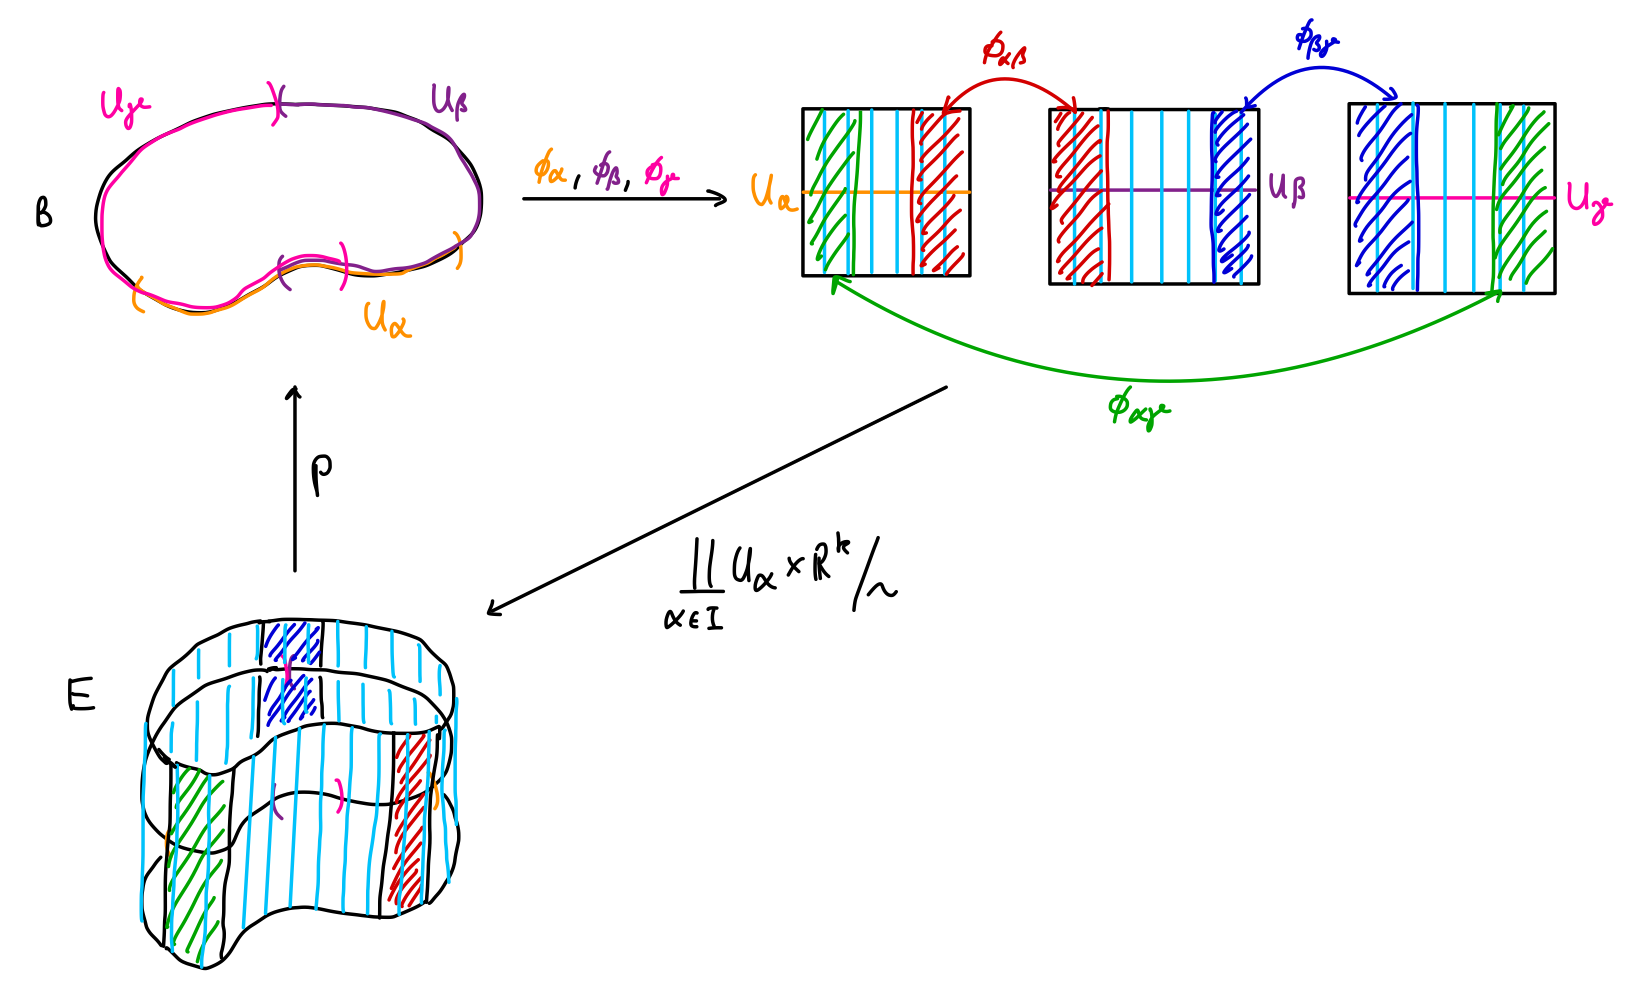
\includegraphics[width=0.5\linewidth]{Bilder/kozykelkonstrukt.png}
\caption{Drei lokale Trivialisierungen können mit Hilfe von Übergangsabbildungen, die die Kozykelbedingung erfüllen, verklebt werden, sodass ein Vektorbündel entsteht.}
\end{figure}
\end{bemerkung}
\begin{beispiele}
\begin{enumerate}
\item Wir betrachten $B = \sph^1 \sub \C$ mit $U_1 := \sph^1 \exc \{-1\}$ und $U_2 := \sph^1 \exc \{1\}$. Insbesondere ist dann $U_1 \cap U_2 = U_+ \cup U_-$. Weiterhin betrachten wir den Spezialfall $k=1$ und die Abbildung
\begin{align}
\phi_{12}: U_1 \cap U_2 &\to \gl{1}{\R} = \R \exc \{0\}\\
z &\mapsto \sgn (\Im (z)) = \begin{cases}
+1 \ \text{auf} \ U_+\\
-1 \ \text{auf} \ U_-
\end{cases}
\end{align}
Das mit diesen Daten konstruierte Bündel hat einen Totalraum, der diffeomorph zu einem offenen \textit{Möbiusband} ist.
\begin{figure}[H]
\label{fig:mobius}
\centering
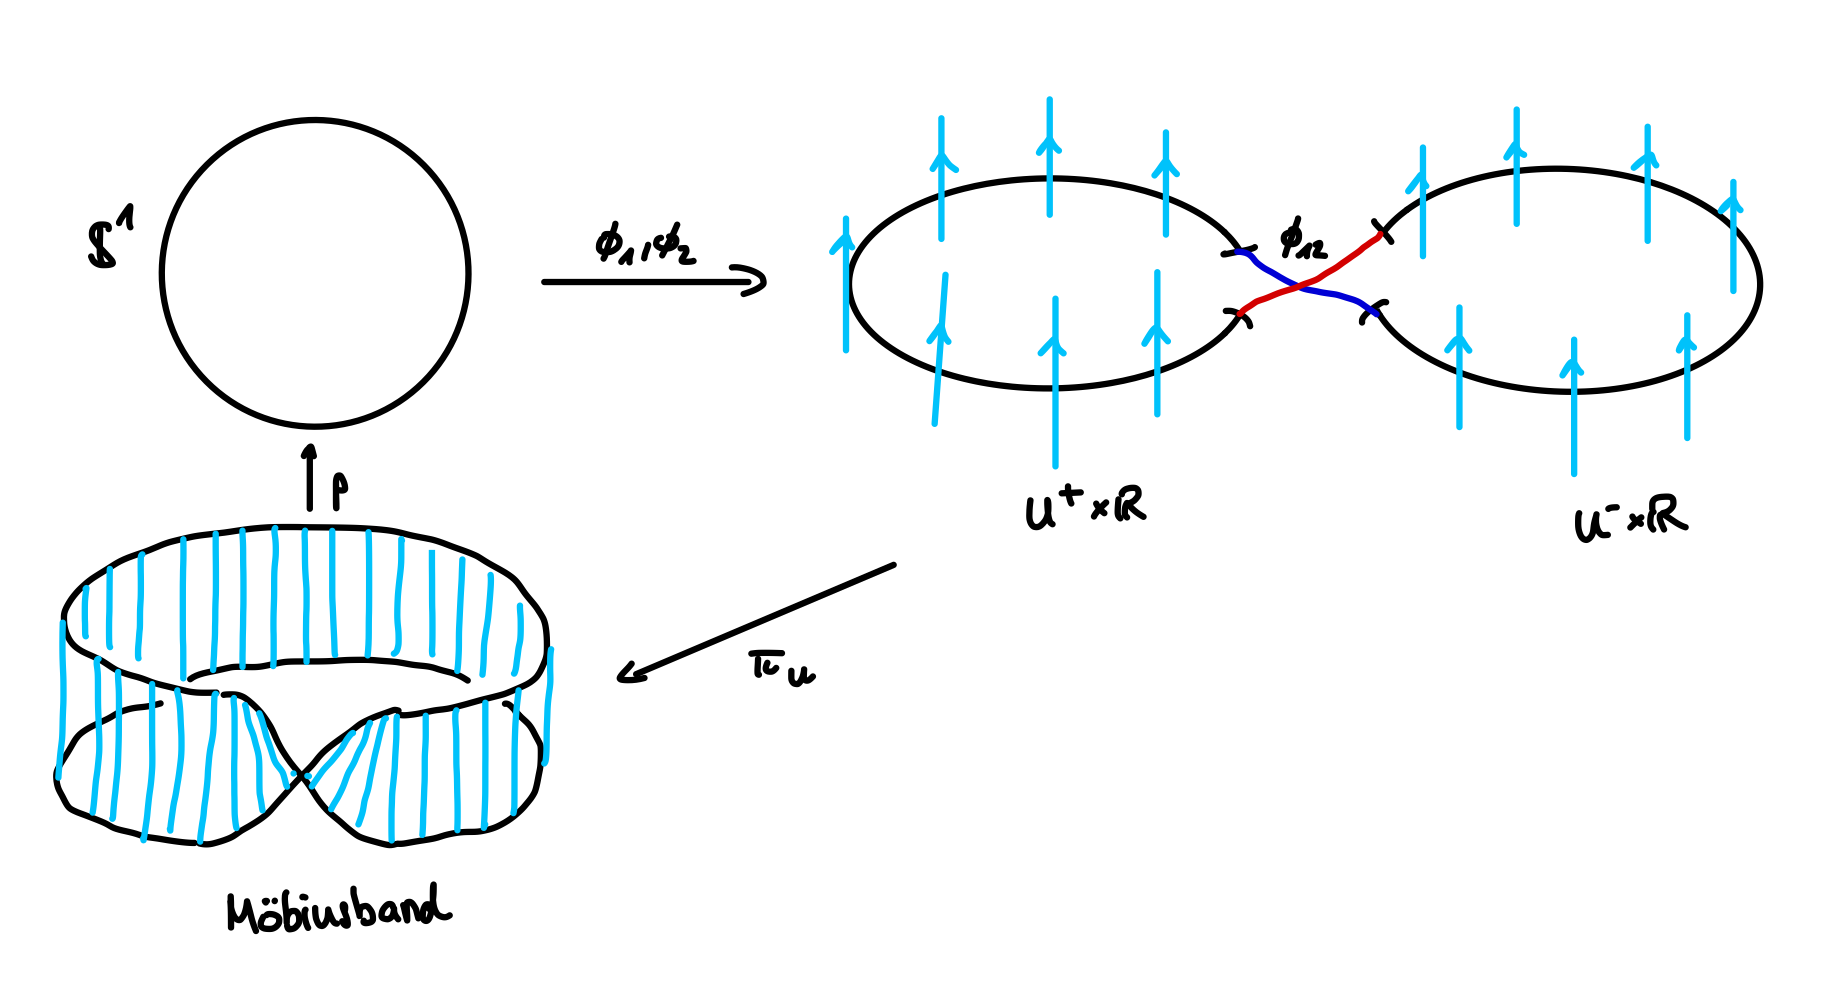
\includegraphics[width=0.4\linewidth]{Bilder/mobius.png}
\caption{Konstruktion des Möbiusbandes durch nichttriviale Verklebung.}
\end{figure}
\item Allgemeiner können wir $B= \sph^n$ mit den offenen Teilmengen $U_1 = \sph^n \exc \{(1,0, \dots, 0 ) \}$ und $U_2 = \sph^n \exc \{(-1, 0, \dots, 0 )\}$ betrachten. dann ist $U_1 \cup U_2 \cong \R^n \exc \{0\}$. Für gegebenes $k \in \N$ und eine glatte Abbildung
\begin{equation}
\rho: \R^n \exc \{0\} \to \gl{k}{\R}
\end{equation}
bestimmt $\rho$ ein Vektorbündel über $\sph^n$ von Rang $k$, indem man $U_1 \times \R^k$ und $U_2 \times \R^k$ über $U_1 \cap U_2 \times \R^k$ mit der Abbildung
\begin{align}
\Psi: (U_1 \cap U_2) \times \R^k &\to (U_1 \cap U_2) \times \R^k \\
(p,v) &\mapsto (p, \rho(p)v)
\end{align}
verklebt.\\
Konkret kann man ein solches $\rho: \R^n \exc \{0\} \to \gl{k}{\R}$ erhalten, indem man zu einer gegebenen Abbildung $\tilde{\rho}: \sph^{n-1} \to \gl{k}{\R}$ die Verknüpfung $\rho = \tilde{\rho} \circ \pi$ mit der Projektion
\begin{align}
\pi: \R^n \exc \{0\} &\to \sph^{n-1} \\
x &\mapsto \frac{x}{||x||}
\end{align}
betrachtet.\\
Für $n=k=2$ können wir mit $m \in \Z$ die Abbildung $\tilde{\rho}_m: \so{2} \cong \sph^1 \to \so{2} \sub \gl{2}{\R}, \ A \mapsto A^m$ betrachten. Auf diese Weise erhält man viele verschiedene Vektorbündel von Rang $2$ über $\sph^2$.  
\end{enumerate}
\end{beispiele}
Wir definieren den Isomorphiebegriff für Vektorbündel:
\begin{definition}{Bündelisomorphismus}{bundiso}
Seien 
\begin{tikzcd}
E_1 \arrow[r, "p_1"] & B_1
\end{tikzcd}
und 
\begin{tikzcd}
E_2 \arrow[r, "p_2"] & B_2
\end{tikzcd}
Vektorbündel. Ein \textbf{Bündelmorphismus} von $(E_1, p_1, B_1)$ zu $(E_2, p_2, B_2)$ besteht aus Abbildungen $f: B_1 \to B_2$ und $F: E_1 \to E_2$, sodass
\begin{center}
\begin{tikzcd}
E_1 \arrow[r, "F"] \arrow[d, "P_1"] & E_2 \arrow[d, "p_2"] \\
B_1 \arrow[r, "f"] & B_2
\end{tikzcd}
\end{center}
kommutiert und
\begin{equation}
F|_{(E_1)_b}: (E_1)_b \to (E_2)_{f(b)}
\end{equation}
linear ist für alle $b \in B_1$.
\end{definition}
\begin{definition}{Isomorphe Vektorbündel}{ismbund}
Zwei Bündel
\begin{tikzcd}
E_1 \arrow[r, "p_1"] & B
\end{tikzcd}
und 
\begin{tikzcd}
E_2 \arrow[r, "p_2"] & B
\end{tikzcd}
über derselben Basis heißen \textbf{isomorph}, falls ein Bündelisomorphismus $(F, f=\id)$ existiert, sodass $F_b: (E_1)_b \to (E_2)_b$ für alle $b \in B$ ein Isomorphismus ist.
\end{definition}
Nach diesem kleinen Exkurs wenden wir uns Tangentialbündeln zu. Das Tangentialbündel an eine glatte MFK $M$ kann man auch durch Verkleben aus lokalen ''Stücken'' erhalten:\\
Zunächst haben wir:
\begin{center}
\begin{tikzcd}
T\R^n = \R^n \times \R^n \arrow[r, "\pi = pr_1"] & \R^n.
\end{tikzcd}
\end{center}
Für $V \sub \R^n$ offen gilt $TV = \pi^{-1}(V) = V \times \R^n$. Ist jetzt $M$ eine glatte MFK der Dimension $n$, so wählen wir einen Atlas $\Af = \{(U_\alpha, \phi_\alpha)\}_{\alpha \in I}$. In unserer ersten Beschreibung von Tangentialräumen hatten wir Tangentialvektoren der Äquivalenzklasse von Tangentialvektoren in Karten definiert. Insbesondere erhalten wir also eine Parametrisierung von 
\begin{align}
\bigcup_{x \in U_\alpha} T_xM &\cong V_\alpha \times \R^n \\
[\phi_\alpha (y, v)] &\mapsfrom (y, v).
\end{align}
Ist $\phi_\beta: U_\beta \to V_\beta \sub \R^n$ eine andere Karte, so ist auf $W=U_\alpha \cap U_\beta$ die Übergangsabbildung
\begin{align}
\psi_{\alpha \beta}: V_\beta \times \R^n \supseteq W \times \R^n &\to W \times \R^n \sub V_\alpha \times \R^n \\
(x, v) &\mapsto \left( x, (\phi_\alpha \circ \phi_\beta^{-1})_{\ast, \phi_\beta(x)} (v) \right).
\end{align}
Aus der Kettenregel folgt, dass diese Übergänge zwischen lokalen Trivialisierungen tatsächlich die Kozykelbedingung erfüllen.\\
Verklebt man also 
$\bigsqcup_{\alpha \in I} U_\alpha \times \R^n$ mit Hilfe der Abbildungen $\psi_{\alpha \beta}$ von oben, erhält man das Tangentialbündel
\begin{tikzcd}
TM \arrow[r, "\pi"] & M.
\end{tikzcd}
\begin{figure}[H]
\label{fig:tangentialbund}
\centering
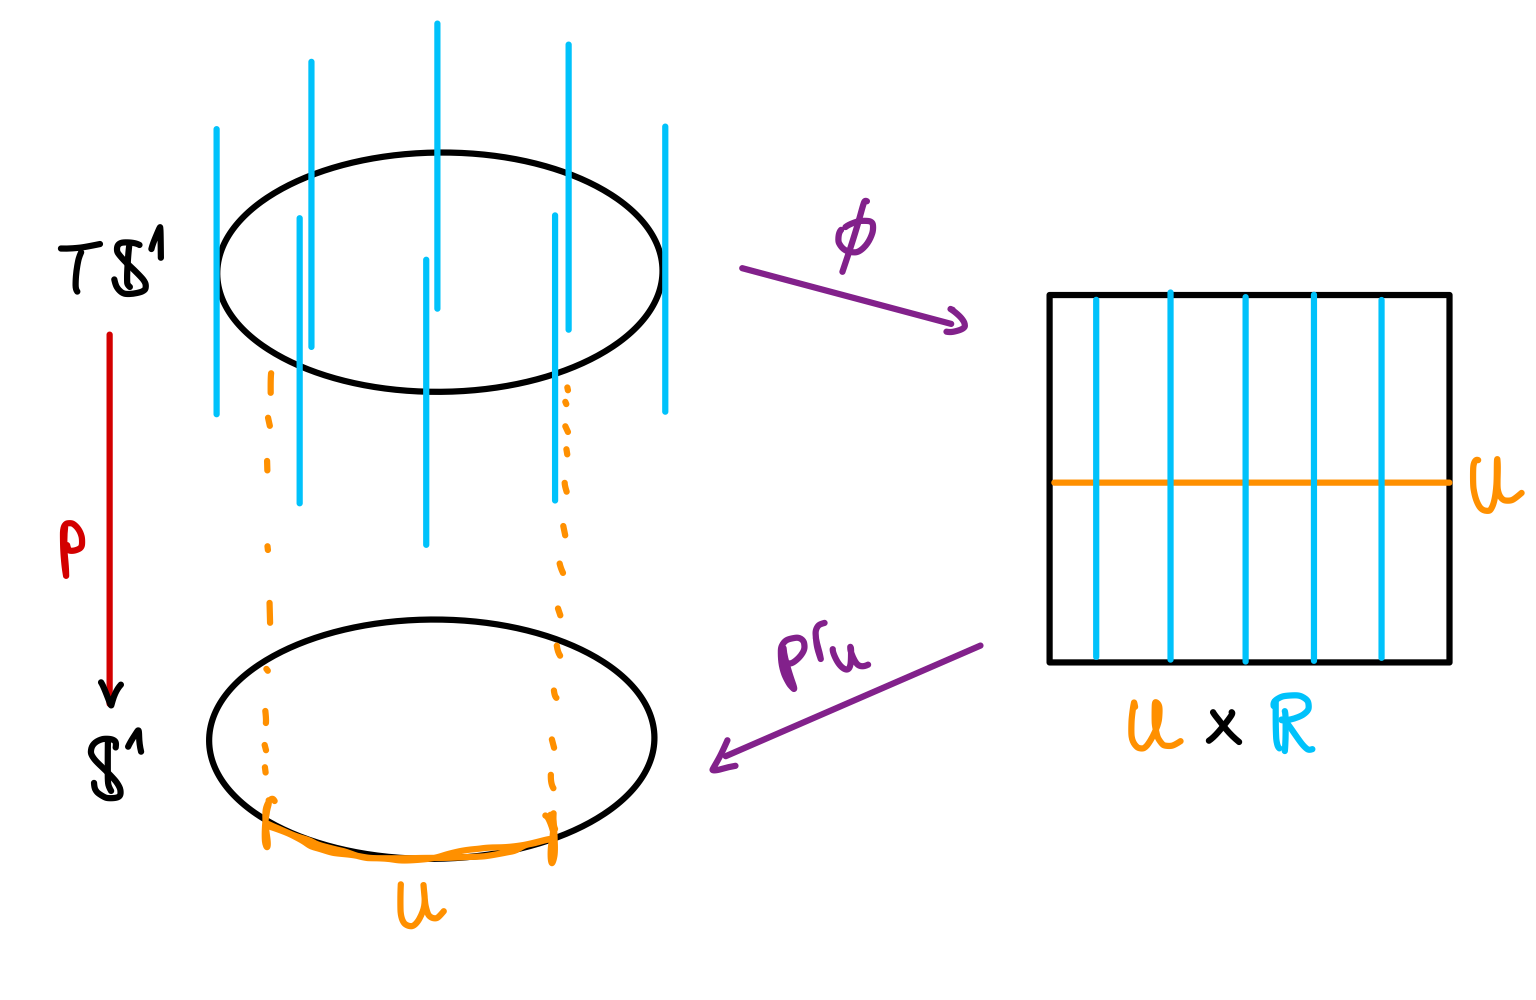
\includegraphics[width=0.4\linewidth]{Bilder/tangentialbundel.png}
\caption{Das Tangentialbündel der Sphäre $\sph^1$ mit lokaler Trivialisierung.}
\end{figure}
\begin{beispiel}Bündelmorphismus\\
Sei $f: M \to N$ eine glatte Abbildung. Dann ist $f_\ast:TM \to TN$ zusammen mit $f$ ein Bündelmorphismus:
\begin{center}
\begin{tikzcd}
TM \arrow[r, "f_\ast"] \arrow[d, "\pi"] & TN \arrow[d, "\pi"] \\
M \arrow[r, "f"] & N
\end{tikzcd}
\end{center}
\end{beispiel}
\begin{definition}{glatter Schnitt}{schnitt}
Sei $p: E \to B$ ein glattes Vektorbündel. Ein \textbf{glatter Schnitt} in $E$ ist eine glatte Abbildung 
\begin{equation}
s: B \to E
\end{equation}
mit $p \circ s = \id_B$.\\
Wir bezeichnen die Menge der Schnitte von $E$ als $\Gamma(E)$.
\begin{figure}[H]
\label{fig:schnitt}
\centering
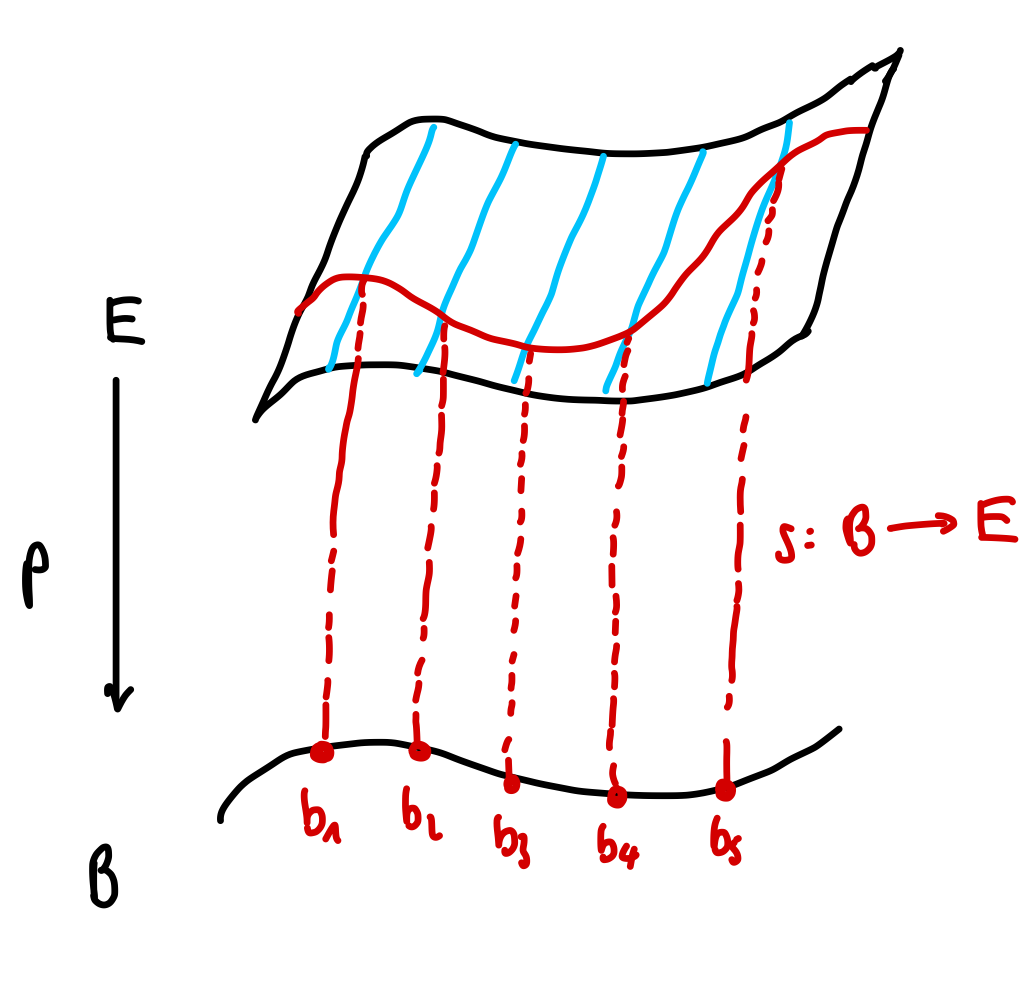
\includegraphics[width=0.3\linewidth]{Bilder/schnitt.png}
\caption{Mehrere Schnitte $s$ wählen zu $b_i$ Vektoren aus $E$ aus.}
\end{figure}
\end{definition}
Ein Schnitt wählt also auf glatte Weise zu jedem $b \in B$ einen Vektor $s(b) \in E_b$ aus. \footnote{Die begriffliche Ähnlichkeit zu Dedekind-Schnitten ist rein zufällig.}
\begin{bemerkungen}Nullschnitt und Vektorraum\\
\begin{enumerate}
\item In jedem Vektorbündel gibt es einen kanonischen Schnitt, der jedem Punkt $b \in B$ den Ursprung des Vektorraums $E_b$ zu. Diesen Schnitt nennt man den \textbf{Nullschnitt} des Bündels.
\item Sind $s_1, s_2 \in \Gamma (E)$, so ist 
\begin{equation}
(s_1+s_2)(b):=s_1(b)+s_2(b)
\end{equation}
wieder ein Schnitt, und für $s \in \Gamma (E)$ und $\lambda \in \R$ ist auch 
\begin{equation}
(\lambda s)(b) := \lambda s(b)
\end{equation}
ein Schnitt. Mit diesen Operationen wird $\Gamma(E)$ zu einem reellen VR.
\item Etwas allgemeiner ist auch für $s \in \Gamma (E)$ und $f \in \cinf{B}{}$ durch
\begin{equation}
(f \cdot s)(b) := f(b) \cdot s(b)
\end{equation}
auch wieder ein Schnitt definiert. Auf diese Weise wird $\Gamma (E)$ zu einem \textit{Modul} über dem Ring $\cinf{B}{}$.
\end{enumerate}
\end{bemerkungen}
\begin{definition}{Vektorfelder}{vekfeld}
(Glatte) Schnitte im Tangentialbündel 
\begin{tikzcd}
TM \arrow[r, "\pi"] & M.
\end{tikzcd}
einer glatten MFK $M$ nennt man \textbf{glatte Vektorfelder auf} $M$.
\begin{figure}[H]
\label{fig:vektorfeldaustang}
\centering
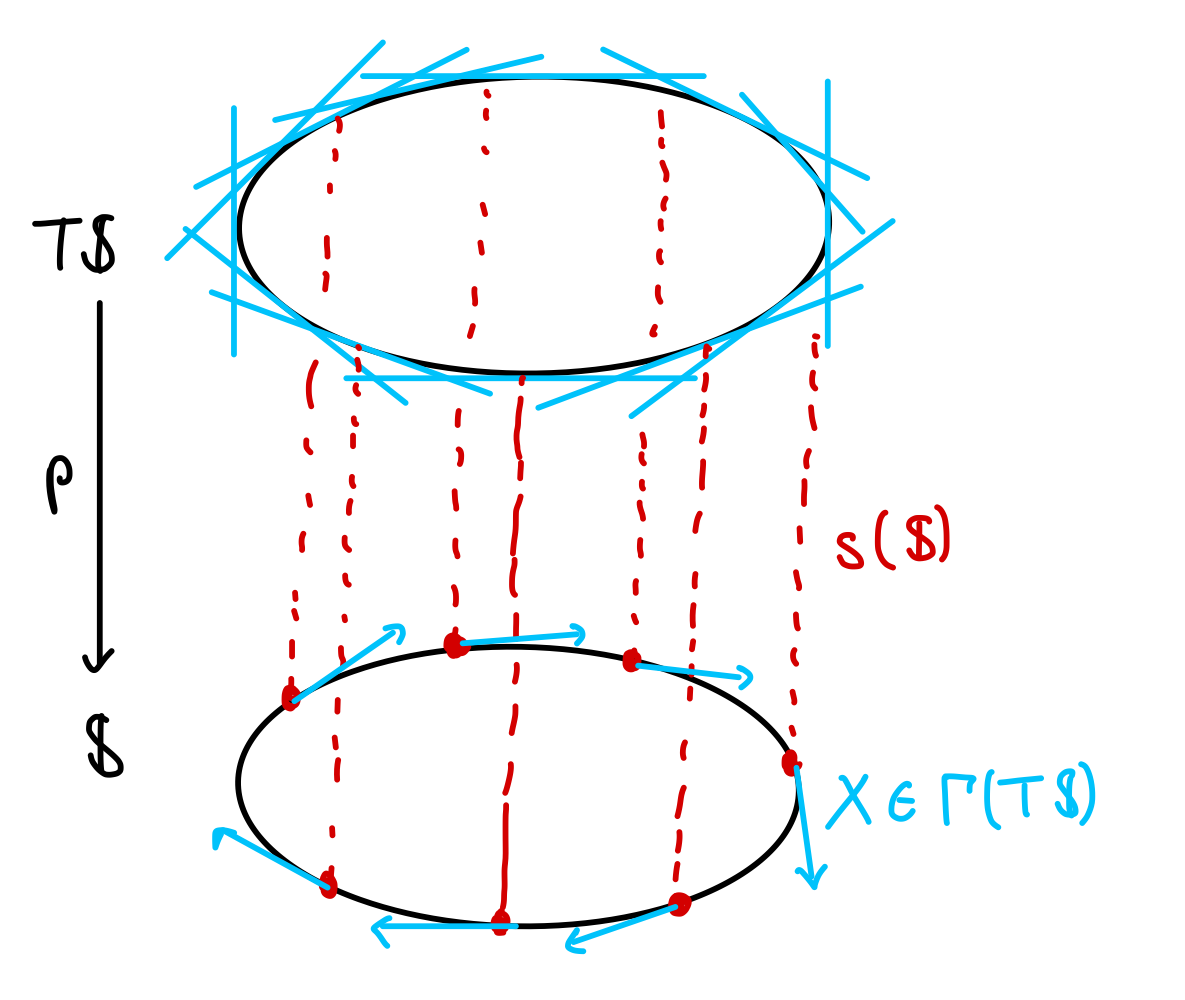
\includegraphics[width=0.3\linewidth]{Bilder/vektorfeldsph.png}
\caption{Aus dem Tangentialbündel von $\sph$ wird ein Vektorfeld ausgewält.}
\end{figure}
\end{definition}
\begin{bemerkung}
Ist $p: E \to B$ ein Vektorbündel und $S \sub B$ eine UMF, so ist
\begin{equation}
p|_{p^{-1}(S)}: p^{-1}(S) (=: E|_S) \to S
\end{equation}
auch ein glattes Vektorbündel.
\end{bemerkung}
\begin{beispiel}
Ist $U \in M$ offen, so gilt $TM|_U = TM$. Hat $S \in M$ positive \textit{Kodimension} (d.h. $\dim S < \dim M$), dann sind die Vektorbündel $TM|_S$ und $TS$ verschieden (da ihr Rang verschieden ist).
\end{beispiel}
Sei $M$ eine glatte MFK und $\phi: U \to V \sub \R^n$ eine lokale Karte mit Koordinaten $(x_1, \dots, x_n)$. Dann definiert die Zuordnung
\begin{align}
\frac{\partial}{\partial x_i}: U &\to TM|_U = TU \\
p &\mapsto \frac{\partial}{\partial x_i}|_p
\end{align}
für jedes $i \in \{1, \dots, n \}$ ein glattes, lokales (d.h. auf $U$ definiertes) Vektorfeld. In der durch die Karte $\phi: U \to V$ bestimmten lokalen Trivialisierung
\begin{equation}
\psi: TM|_U \to TV = V \times \R^n
\end{equation}
entspricht $\frac{\partial}{\partial x_i}$ dem konstanten Vektorfeld
\begin{equation}
p \mapsto \left( \phi(p), (0, \dots, 1, 0, \dots, 0)\right).
\end{equation}
In jedem $p \in U$ bilden die Vektoren $\frac{\partial}{\partial x_1}|_p, \dots, \frac{\partial}{\partial x_n}|_p$ eine Basis von $T_pM$. Es ist dann klar, dass jedes auf $U$ definiertes Vektorfeld sich als Linearkombination der $\frac{\partial}{\partial x_i}$ mit Koeffizienten in $\mathcal{C}^\infty (M)$ schreiben lässt.
\begin{satz}{}{}
Sei $\phi: U \to V \sub \R^n$ eine Karte für $M$ mit lokalen Koordinaten $(x_1, \dots, x_n)$. Dann hat jedes lokal definierte, glatte Vektorfeld $X \in \Gamma(TM|_U)$ die Darstellung
\begin{equation}
X(p) = \Sum{i,1,n} X(x_i) \cdot \left.\frac{\partial}{\partial x_i}\right|_p \ (\ast)
\end{equation}
mit der Derivation $X_p(x_i) =: X(x_i)(p)$ im Punkt $p$.\\
Umgekehrt wird für beliebige Funktionen $f_1, \dots, f_n \in \cinf{U}{}$ durch
\begin{equation}
fX := \Sum{i,1,n} f_i \frac{\partial}{\partial x_i}
\end{equation}
ein glattes, lokales Vektorfeld definiert.
\begin{figure}[H]
\label{fig:normalformvek}
\centering
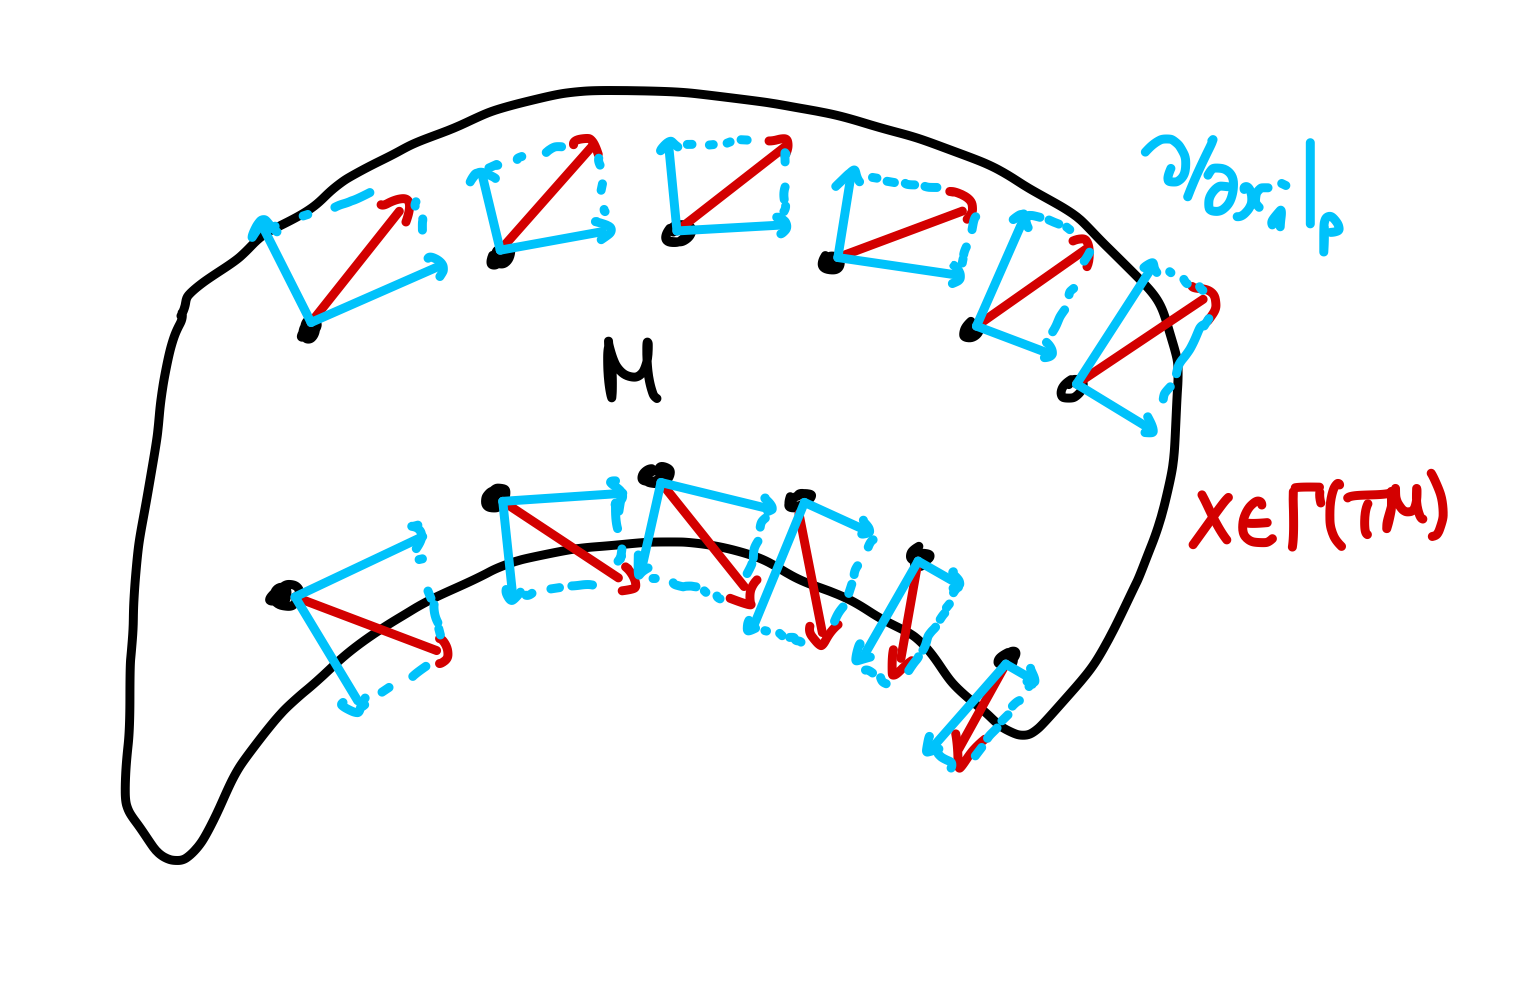
\includegraphics[width=0.25\linewidth]{Bilder/normalformvek.png}
\caption{Die Normalform eines Vektorfeldes.}
\end{figure}
\end{satz}
\begin{beweis}
Die punktweise Formel $(\ast)$ hatten wir uns bereits überlegt, als wir über Tangentialvektoren als punktweise Derivationen gesprochen haben.\\
Die Funktionen $X(x_i)$ sind glatt, weil sie die Darstellung von $X$ in der lokalen Trivialisierung durch $\left( \frac{\partial}{\partial x_1}, \dots, \frac{\partial}{\partial x_n} \right)$ beschreiben.\\
Die letzte Aussage ist offensichtlich.
\end{beweis}
\begin{bemerkungen}
\begin{enumerate}
\item Ist $p: E \to B$ ein Vektorbündel von Rang $k$, $U \in B$ eine offene Menge und $s_1, \dots, s_k: U \to E|_U$ Schnitte von $E$ über $U$, sodass in jedem Punkt $b \in U$ die Vektoren $s_1(b), \dots, s_k(b)$ eine Basis der Faser $E_b$ bilden, so nennt man $(s_1, \dots, s_k)$ einen \textbf{lokalen Rahmen} für $E$.\\
Jede lokale Trivialisierung gibt einen solchen lokalen Rahmen, und umgekehrt bestimmt auch jeder lokale Rahmen für $E$ eine lokale Trivialisierung von $E$.
\item Man nennt ein Vektorbündel \textbf{trivial}, falls ein globaler Rahmen existiert, d.h. falls es isomorph zum Bündel $B \times \R^k \to B$ ist.
\end{enumerate}
\end{bemerkungen}
\begin{bemerkung}
Zu jeder Konstruktion mit Vektorräumen gibt es eine zugehörige Konstruktion mit Vektorbündeln über einer festen Basis.
\begin{beispiel}
Jeder Vektorraum hat einen Dualraum (und lineare Abbildungen $L: V \to W$ induzieren duale Abbildungen $L^\ast: W \to V$). Analog kann man für jedes Vektorbündel 
\begin{tikzcd}
E \arrow[r, "p"] & B
\end{tikzcd}
ein duales Bündel 
\begin{tikzcd}
E^\ast \arrow[r, "p"] & B
\end{tikzcd}
konstruieren, sodass $(E^\ast)_b = (E_b)^\ast$ gilt. Wendet man diese Überlegungen auf $TM \to M$ an, so erhält man das \textit{Kotangentialbündel} $T^\ast M \to M$.\\
 Dual zur lokalen Basis von Vektorfeldern $\left( \frac{\partial}{\partial x_1}, \dots, \frac{\partial}{\partial x_n}\right)$ hat man eine lokale Basis von $1$-Formen $\left( dx_1, \dots, dx_n \right)$.\\
Dual zum Differential $f_\ast: TM \to TN$ einer Abbildung $f: M \to N$ erhalten wir $f^\ast: T^\ast N \to T^\ast M$ (Zurückziehen von $1$-Formen).
\end{beispiel}
\end{bemerkung}
\begin{definition}{Algebra}{alg}
Eine \textbf{Algebra über} $\R$ ist ein $\R$-Vektorraum $A$ mit einer Multiplikation
\begin{equation}
\cdot: A \times A \to A,
\end{equation}
die bilinear ist, es gilt also
\begin{gather}
(a_1 + a_2) \cdot b = a_1b + a_2b \\
a(b_1+b_2) = ab_1 + ab_2\\
\forall \lambda \in \C (\lambda a)b = \lambda (ab) = a \cdot (\lambda b).
\end{gather}
\end{definition}
\begin{bemerkung}
Mit punktweiser Addition ist der Raum $\cinf{M}{\R}$ ein $\R$-Vektorraum. Mit der punktweisen Multiplikation wird dieser zu einer Algebra über $\R$.
\end{bemerkung}
\begin{definition}{Derivation reloaded}{dervneu}
Eine \textbf{Derivation} auf $A$ ist eine $\R$-lineare Abbildung
\begin{equation}
\Df: A \to A
\end{equation}
mit $\Df (ab) = \Df (a) b + a \Df (b)$.\\
Die Derivationen auf $A$ bilden einen reellen Vektorraum $\der{p}$.
\end{definition}
\begin{satz}{Isomorpie von $\Gamma$ und $\text{Der} (\text{C}^\infty)$}{isomorphveccinf}
Sei $M$ eine glatte MFK. Der reelle Vektorraum der Vektorfelder $\Gamma (TM)$ auf $M$ ist auf natürliche Weise\footnote{Natürlich heißt, dass wir keine konkrete, nicht-kanonische Wahl für den Isomorphismus treffen müssen.} isomorph zum Vektorraum $\text{Der}(\cinf{M})$.
\end{satz}
\begin{beweis}
Da Vektorfelder punktweise Tangentialvektoren sind, wird für $X \in \Gamma (TM)$ und $f \in \cinf{M}$ durch
\begin{equation}
(Xf)(p):= \underbrace{X_p}_{\in T_pM} f
\end{equation}
eine Funktion $Xf: M \to \R$ definiert. In lokalen Koordinaten rechnet man leicht nach, dass diese Funktion glatt ist. Dazu nutzt man die Darstellung $X=\sum_i X_i \frac{\partial}{\partial x_i}$ und wendet sie auf $f$ an, was eine Summe glatter Funktionen liefert.\\
Außerdem ist die Zuordnung
\begin{align}
\cinf{M} &\to \cinf{M} \\
f &\mapsto Xf
\end{align}
linear über $\R$, d.h. für $\lambda, \mu \in \R$ und $f, g \in  \cinf{M}$ gilt $X(\lambda f + \mu g)=\lambda X f + \mu X g$. Auch die Leibnizregel $X(f \cdot g)= (Xf) \cdot g + f \cdot (Xg)$ ist erfüllt. Also wird auf diese Weise jedem Vektorfeld $X \in \Gamma (TM)$ eine Derivation $\Df_x \in \text{Der} (\cinf{M})$ zugeordnet, nämlich $\Df_X (f) = Xf$. Die Abbildung $\Gamma (TM) \to \text{Der} (\cinf{M})$ ist offensichtlich linear.\\
Ist umgekehrt $\Df \in \text{Der} (\cinf{M})$, so erhalten wir durch Auswertung in $p \in M$ einen Tangentialvektor $X_\Df (p) \in \der{p} \cong T_pM$. Diese Zuordnung definiert einen Schnitt
\begin{align}
M &\to TM \\
p &\mapsto X_\Df (p).
\end{align}
Da $\Df f$ für alle $f \in \cinf{M}$ wieder glatt ist, gilt dies insbesondere auch für (geeignet abgeschnittene) lokale Koordinatenfunktionen $x_i$. Also hat $X_\Df$ die lokale Darstellung
\begin{equation}
X_\Df |_U = \Sum{i,1,n} \Df (x_i) \frac{\partial}{\partial x_i}
\end{equation}
mit glatten Koeffizienten $\Df (x_i)$. Also ist $X_D$ ein glattes Vektorfeld.\\
Da diese beiden Abbildungen offensichtlich invers zueinander sind, sind sie Isomorphismen zwischen $\Gamma (TM)$ und $\text{Der} (\cinf{M})$.
\end{beweis}
Wir nutzen hier eine sehr abstrakte Sichtweise, da wir dadurch eine zusätzliche algebraische Struktur auf $\Gamma (TM)$ erhalten. Dazu erst ein paar algebraische Vorüberlegungen:
\begin{bemerkung}
Ist $A$ eine $\R$-Algebra und $\Df_1, \Df_2 \in \text{Der}(A)$, so gilt:
\begin{align}
\Df_1 \Df_2 (ab) &= \Df_1 (\Df_2 (a)b+ a \Df_2(b))\\
&=(\Df_1 \Df_2 (a))b + \Df_2(a)\cdot \Df_2(b) + \Df_1 (a) \cdot \Df_2 (b) + a (\Df_1 \Df_2 (b))
\end{align}
Wir beobachten, dass $\Df_1 \Df_2$ \textit{keine} Derivation ist, aber die Störterme symmetrisch in $\Df_1$ und $\Df_2$ sind.
\end{bemerkung}
\begin{definition}{Kommutator}{komm}
Für $\Df_1, \Df_2 \in \text{Der} (A)$ ist der \textbf{Kommutator} gegeben durch
\begin{equation}
[\Df_1, \Df_2] := \Df_1 \Df_2 - \Df_2 \Df_1.
\end{equation}
\end{definition}
Der Kommutator ist also für $\Df_1, \Df_2 \in \text{Der} (A)$ wieder eine Derivation.
\begin{satz}{Kommutator als Lie-Algebra}{liederp}
Sei $A$ eine $\R$-Algebra. Dann ist $\text{Der} (A)$ mit dem Kommutator
\begin{equation}
[., .]: \text{Der} (A) \times \text{Der} (A) \to \text{Der} (A),
\end{equation}
auch \textbf{Lie-Klammer} genannt, eine \textit{Lie-Algebra}. Es gilt somit:
\begin{itemize}
\item $[., .]$ ist $\R$-bilinear.
\item $[., .]$ ist \textit{schiefsymmetrisch}: $ [ \Df_2, \Df_1] = - [\Df_1, \Df_2 ]$.
\item Es gilt die \textit{Jacobi-Identität}: $[\Df_1, [\Df_2, \Df_3]] + [\Df_2, [\Df_3, \Df_1]] + [\Df_3, [\Df_1, \Df_2]] = 0$.
\end{itemize}
\end{satz}
\begin{beweis}
Die ersten beiden Bedingungen folgen direkt aus der Definition. Für die dritte Bedingung muss man nachrechnen: $[\Df_1, [\Df_2, \Df_3]] = [\Df_1, \Df_2\Df_3-\Df_3\Df_2]$. Also gilt
\begin{align}
[\Df_1, [\Df_2, \Df_3]] &= \Df_1\Df_2\Df_3 - \Df_2\Df_3\Df_1-\Df_1\Df_3\Df_2 + \Df_3\Df_2\Df_1\\
[\Df_2, [\Df_3, \Df_1]] &= \Df_2\Df_3\Df_1 - \Df_3\Df_1\Df_2-\Df_2\Df_1\Df_3 + \Df_1\Df_3\Df_2.
\end{align}
\end{beweis}
\begin{korollar}{Glatte VF als Lie-Algebra}{gvflie}
Auf jeder glatten MFK $M$ bilden die glatten Vektorfelder $\Gamma (TM)$ mit dem Kommutator eine Lie-Algebra.
\end{korollar}
\begin{beweis}
Für lokale Koordinatenvektorfelder $\fracpart{x}, \frac{\partial}{\partial x_j}$ gilt
\begin{equation}
\left[ \fracpart{x}, \frac{\partial}{\partial x_j} \right] =0.
\end{equation}
Übung (A12).
\end{beweis}
\begin{satz}{Differential und Lie-Klammer}{difflieklammer}
Seien $M, N$ glatte MFK und $F: M \to N$ eine glatte Abbildung. Gilt für $X_1, X_2 \in \Gamma(TM)$ und $\bar{X}_1, \bar{X}_2$ an jedem Punkt $p \in M$ die Beziehung
\begin{equation}
(\bar{X}_i)_{F(p)} = F_\ast (X_i)_p,
\end{equation}
so gilt auch
\begin{equation}
[\bar{X}_1, \bar{X}_2]_{F(p)} = F_\ast [X_1, X_2]_p
\end{equation}
für alle $p \in M$.
\end{satz}
\begin{beweis}
Übung (A12)
\end{beweis}
\begin{definition}{Integralkurve}{intkurv}
Sei $M$ eine glatte MFK und $X \in \Gamma (TM)$ ein glattes Vektorfeld.\\
Eine Kurve $c: [a,b] \to M$ heißt \textbf{Integralkurve} für $X$, falls für alle $t \in (a,b)$ gilt:
\begin{equation}
\dot{c}(t) = X_{c(t)}.
\end{equation}
\begin{figure}[H]
\label{fig:integralkurve}
\centering
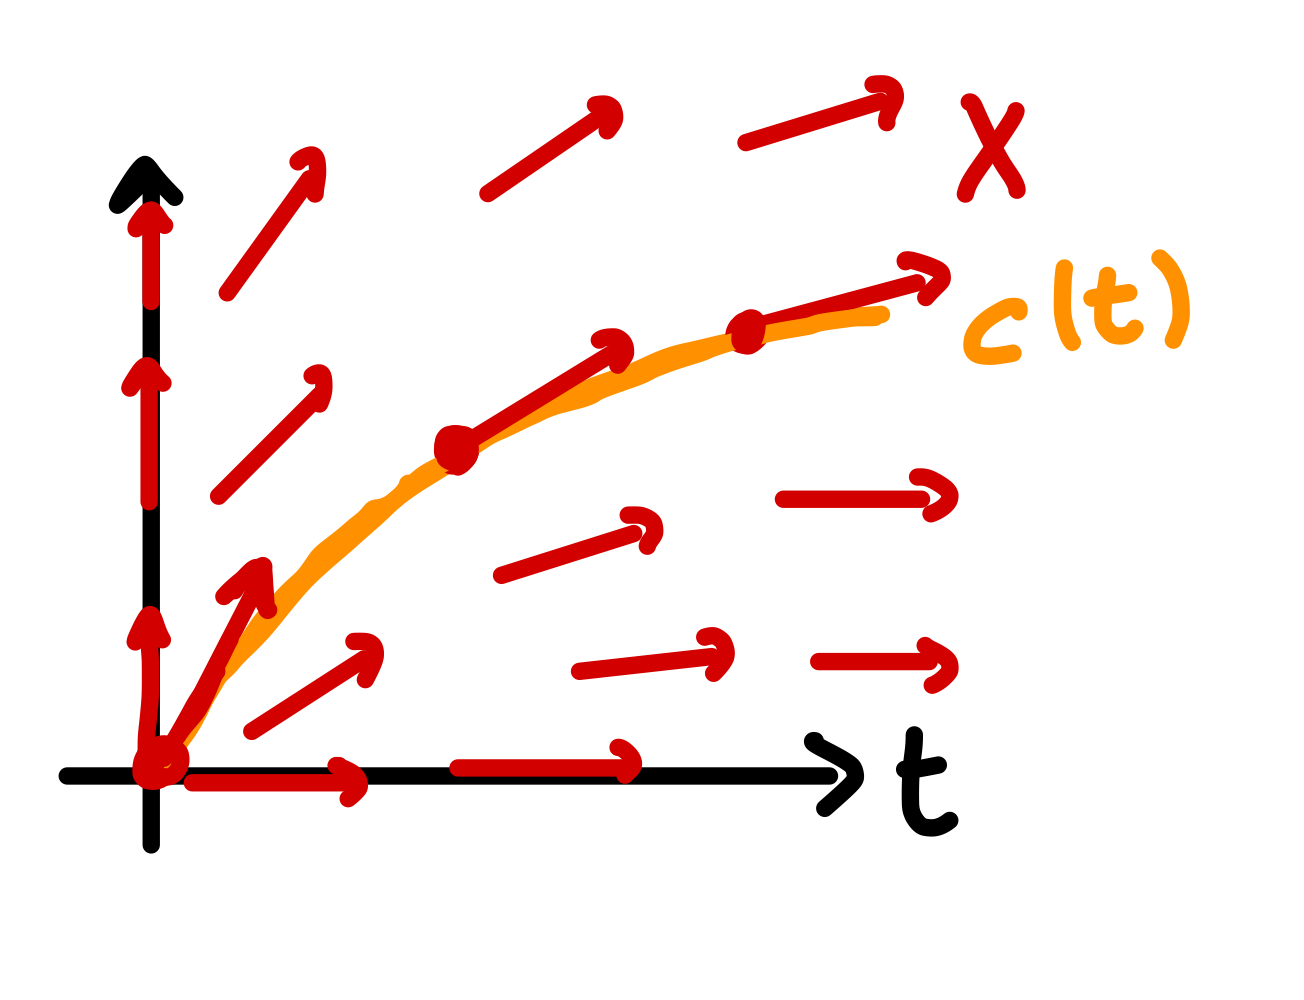
\includegraphics[width=0.25\linewidth]{Bilder/integralkurve.png}
\caption{Eine Integralkurve $c(t)$ eines Vektorfeldes $X$.}
\end{figure}
\end{definition}
In lokalen Koordinaten nahe $c(t_0) \in M$ wird diese Bedingung zu einer gewöhnlichen DGL 1. Ordnung für die Koordinaten der Kurve.
\begin{bemerkung}
Aus der allgemeinen Theorie der Differentialgleichungen erhalten wir zu jedem $p \in M$ ein maximales Intervall $0 \in I_p \sub \R$ offen, sodass eine Integralkurve $c: I_p \to M$ mit $c(0) =p$ existiert.
\end{bemerkung}
Wir definieren jetzt 
\begin{equation}
\Ds_X := \{ (p,t) \in M \times \R | t \in I_p \} \sub M \times \R.
\end{equation}\\
\begin{satz}{Maximale Lösungen für Integralkurven}{maxsol}
Sei $M$ eine glatte MFK und $X \in \Gamma (TM)$. Dann gilt:
\begin{itemize}
\item $\Ds_X \sub M \times \R$ ist offen.
\item $\Phi: \Ds_X \to M, \ (p,t) \mapsto c_p(t)$ ist glatt, wobei $c_p: I_p \to M$ die maximale Integralkurve durch $p$ ist.
\item Für $p \in M$ und $q = \Phi (p,t)$ gilt $I_q = I_p -t$ und $\Phi(p, s+t) = \Phi(\Phi(p,t), s) = \Phi(q, s)$, sobald einer der Terme definiert ist.
\end{itemize}
\begin{figure}[H]
\label{fig:maxlsg}
\centering
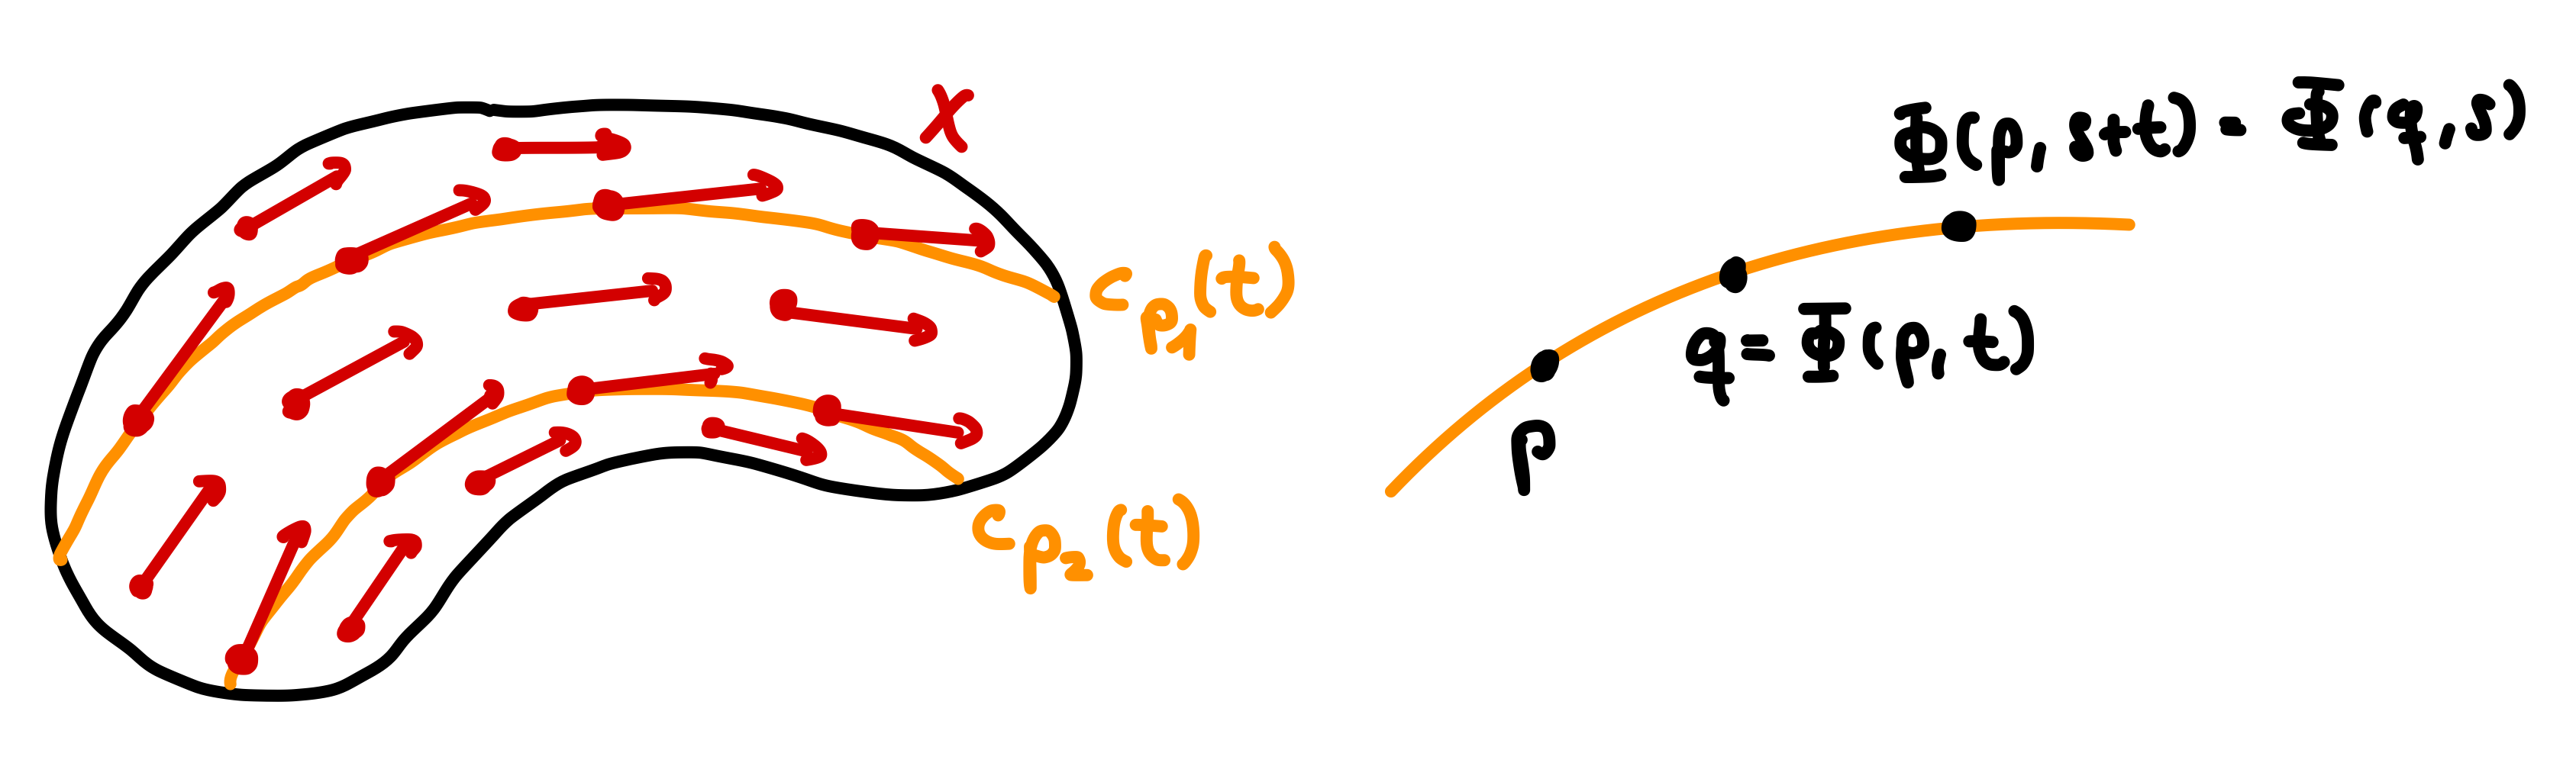
\includegraphics[width=0.5\linewidth]{Bilder/maxlsg.png}
\caption{Die Integralkurven auf einer MFK und die Funktion $\Phi$.}
\end{figure}
\end{satz}
\begin{beweis}
Die erste Bedingung folgt aus dem Satz von Picard-Lindelöf. Die zweite Bedingung folgt aus einem Satz über ODEs. Die letzte Bedingung ist ein Eindeutigkeitssatz.
\end{beweis}
\begin{definition}{Vollständigkeit}{vollst}
Ein Vektorfeld $X$ auf $M$ heißt \textbf{vollständig}, falls $\Ds_X = M \times \R$ gilt, also für jedes $p \in M$ die maximale Integralkurve durch $p$ für alle Zeiten $t \in \R$ definiert ist.
\end{definition}
\begin{bemerkungen}
\begin{enumerate}
\item Aus der lokalen Lösungstheorie erhält man, dass jedes Vektorfeld auf einer unberandeten, kompakten MFK vollständig ist.
\item Wir definieren den \textbf{Träger von} $X$ als $\supp X = \overline{\{ p \in M | X_p \neq 0 \}}$. Jedes Vektorfeld mit kompaktem Träger ist vollständig.
\begin{figure}[H]
\label{fig:kompaktesfeld}
\centering
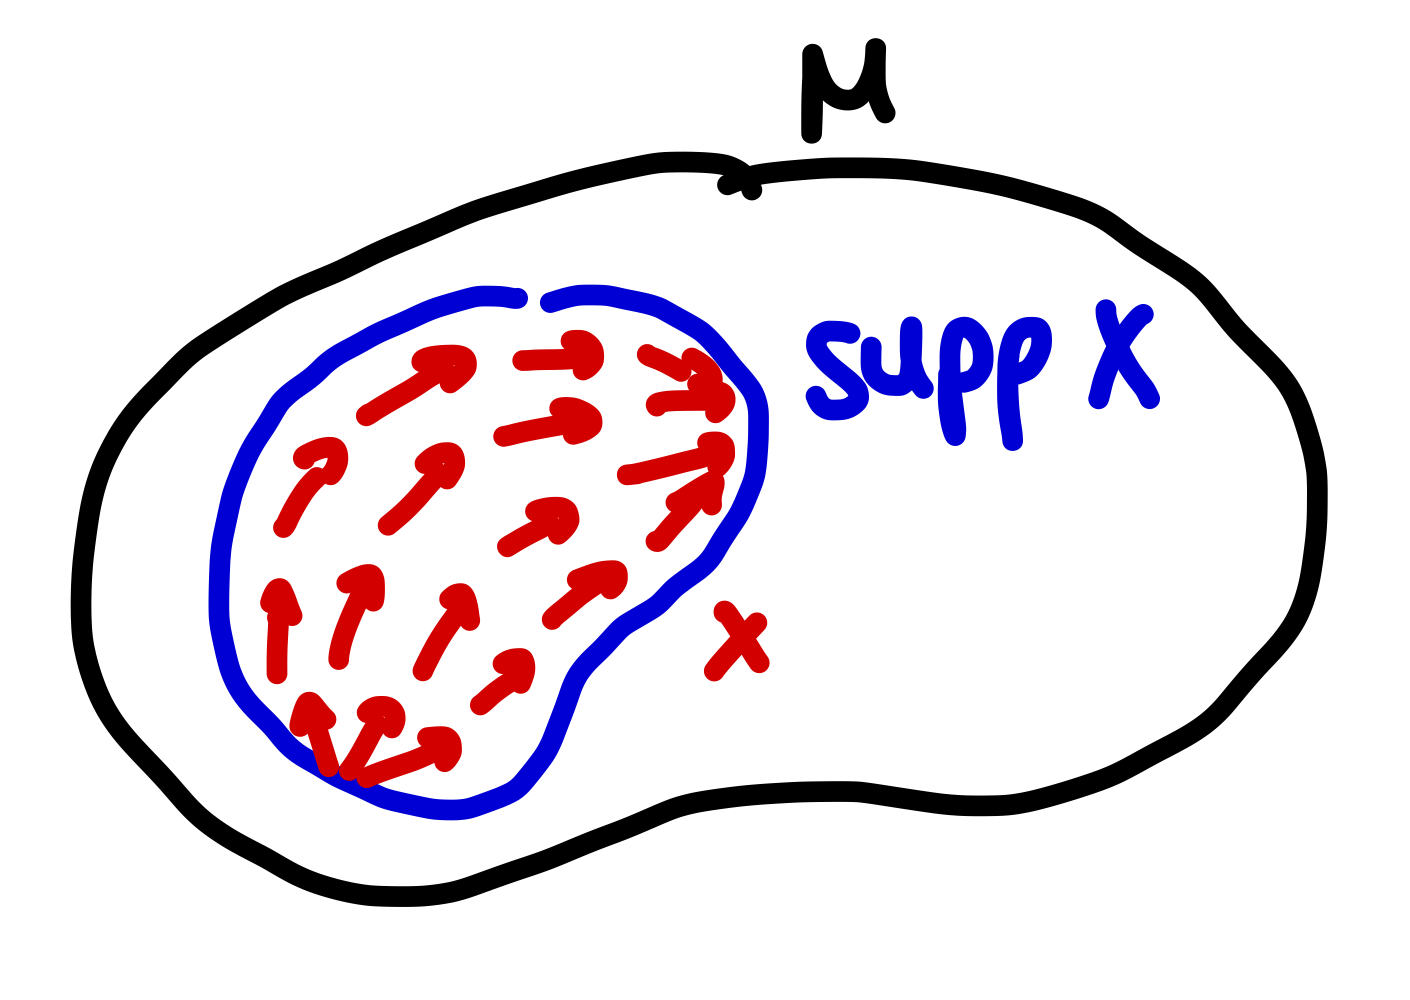
\includegraphics[width=0.2\linewidth]{Bilder/kmpktvektor.png}
\caption{Ein Vektorfeld mit kompaktem Träger.}
\end{figure}
\end{enumerate}
\end{bemerkungen}
\begin{beispiele}
\begin{enumerate}
\item Auf $M = \R^2$ betrachten wir das Vektorfeld
\begin{equation}
X_{(x,y)} := x \frac{\partial}{\partial y} - y \frac{\partial}{\partial x}.
\end{equation}
Dieses Vektorfeld ist vollständig mit
\begin{equation}
\Phi \left( \cvc{x,y}, t \right) = \mat{\cos t, - \sin t}{\sin t, \cos t}\cvc{x,y}.
\end{equation}
Entfernt man eine abgeschlossene Teilmenge $A \sub \R^2$ wie im Bild, so ist die Einschränkung von $X$ auf $\R^2 \times A$ nicht mehr vollständig.
\begin{figure}[H]
\label{fig:vektorfeldbsp}
\centering
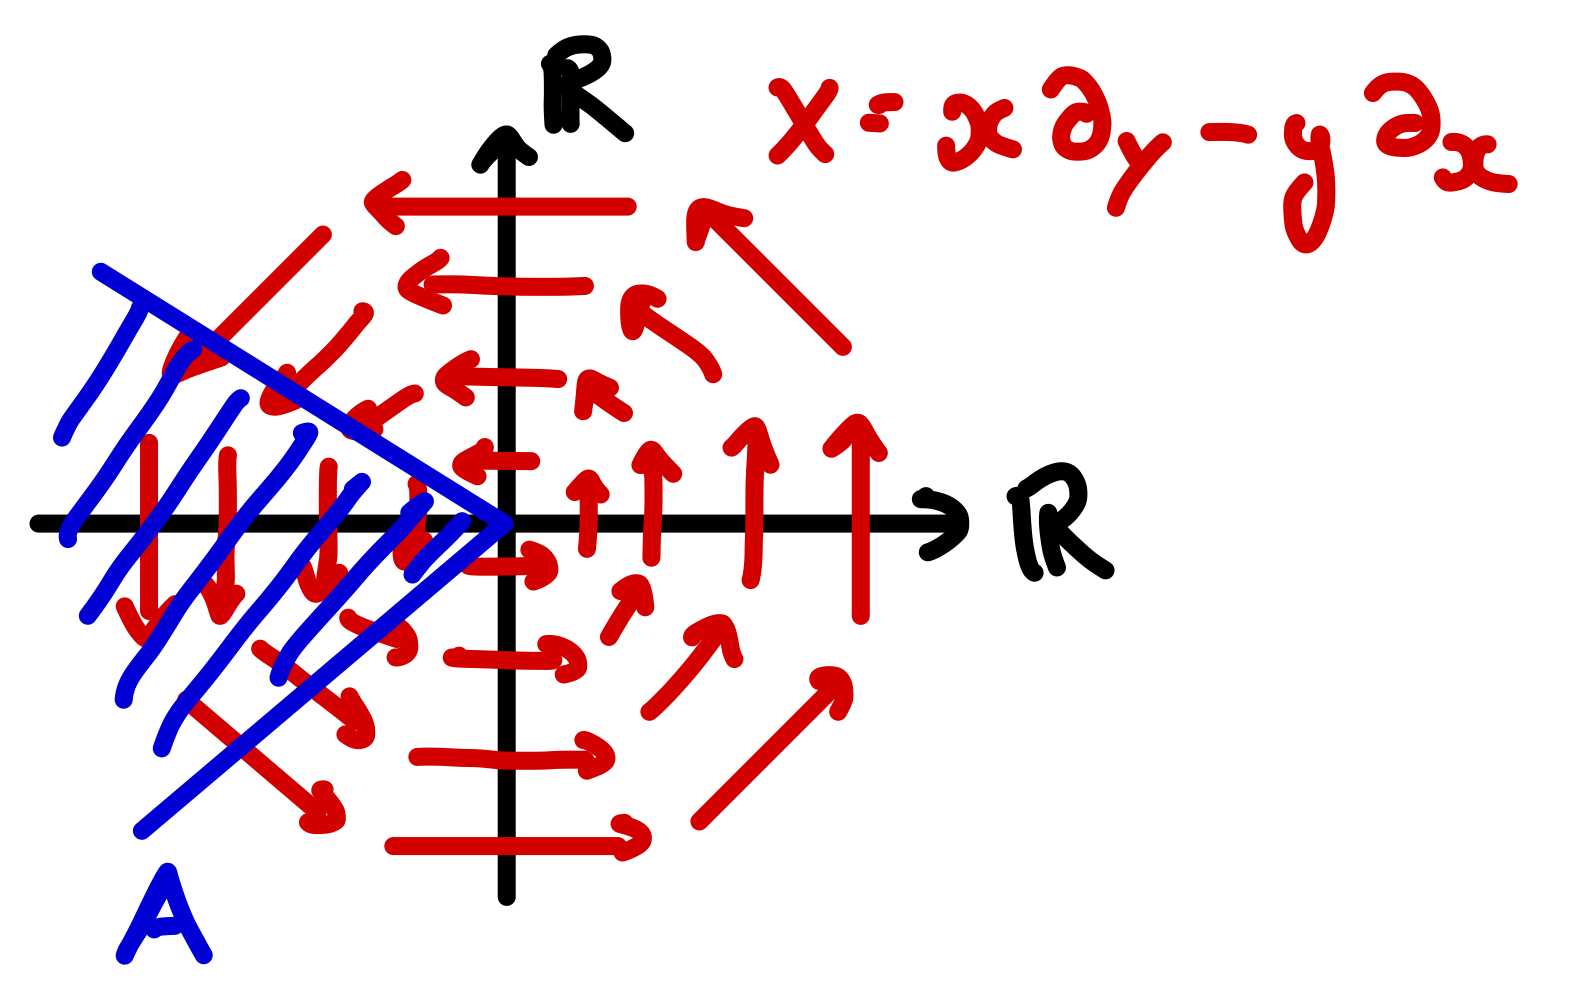
\includegraphics[width=0.2\linewidth]{Bilder/vektorfeldbsp.png}
\caption{Das Vektorfeld $X_{(x,y)}$ mit einer entnommenen Teilmenge $A \sub \R^2$.}
\end{figure}
\item Wir betrachten $M \sub \sph^2 \sub \R^3$ und wählen $v \in \sph^2$ fest. Wir definieren nun Vektorfelder $X$ und $Y$ auf $\sph^2$ als $X_p := v \times p$ und $Y_p := X_p \times p = (v \times p) \times p$.\footnote{$\times$ ist hier das Kreuzprodukt.} 
\end{enumerate}
\end{beispiele}
Hier ist es sinnvoll, den Einschub zur Lösungstheorie von ODEs anzuschauen.
\begin{satz}{Einparametergruppe von Diffeomorphismen}{einparameterdiff}
Sei $M$ eine glatte MFK und $X \in \Gamma(TM)$ vollständig, d.h. $I_p = \R$ für alle $p$. Die Abbildung
\begin{align}
\Phi: M \times \R &\to M \\
(p,t) &\mapsto c_p(t)
\end{align}
ist global definiert, wobei $c_p: I_p \to M$ die Integralkurve von $X$ mit $c_p(0)=p$ ist. Für $t \in \R$ fest erhalten wir:
\begin{align}
\phi_t: M &\to M \\
p &\mapsto \Phi(p,t).
\end{align}
Es gilt $\phi_0 =\id$ und $\phi_{t+s}=\phi_t\phi_s$. Insbesondere ist $\phi_t: M \to M$ invertierbar mit $(\phi_t)^{-1}=\phi_{-t}$.\\
Das bedeutet: Die Abbildung
\begin{align}
\R &\to \text{Diff}(M)\\
t &\mapsto \phi_t
\end{align}
ist ein \textit{Gruppenhomomorphismus}. Man nennt das Bild die zum Vektorfeld $X$ gehörende \textbf{Einparametergruppe} von Diffeomorphismen. $\phi_t$ heißt \textbf{Fluss} des Vektorfeldes $X$.
\begin{figure}[H]
\label{fig:fluss}
\centering
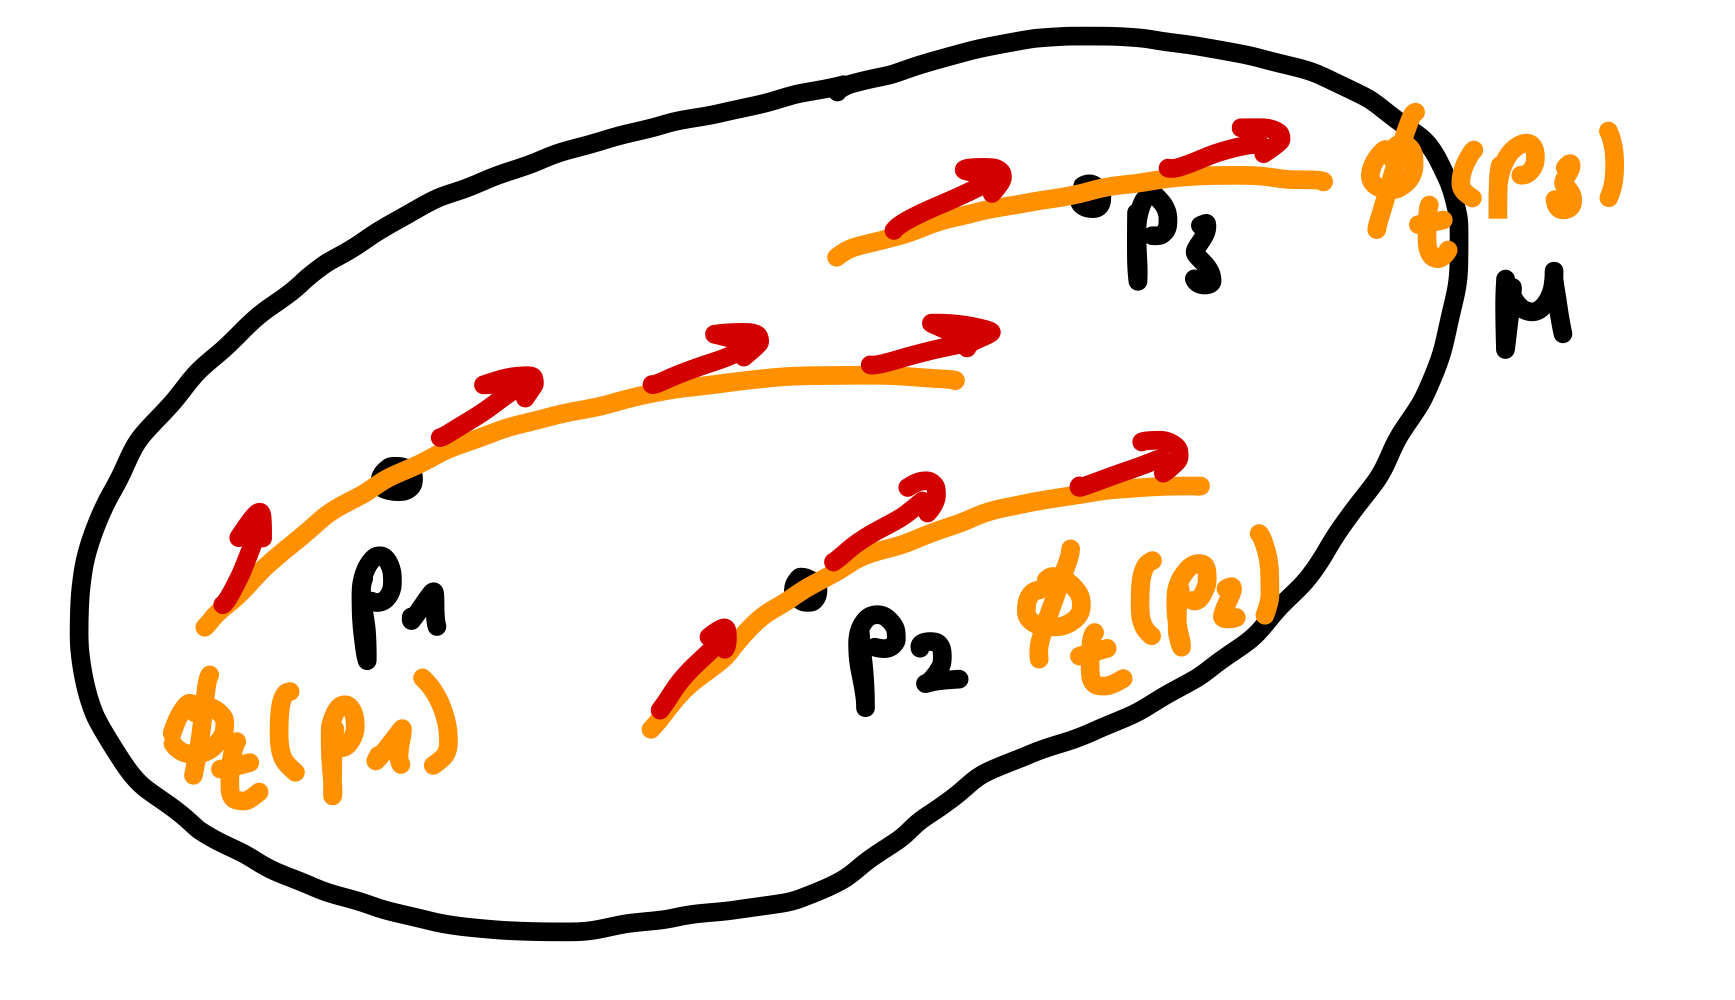
\includegraphics[width=0.25\linewidth]{Bilder/diffgruppe.png}
\caption{Die Diffeomorphismen ordnen jedem Punkt auf der MFK einen Punkt auf einer Integralkurve zu.}
\end{figure}
\end{satz}
\begin{bemerkung}
Ist umgekehrt $h: \R \to \text{Diff}(M)$ ein Gruppenhomomorphismus, sodass die Abbildung $\Psi: M \times \R \to M, \ (p, t) \mapsto h(t)(p)$ glatt ist, so kommt $h$ auch von einem Vektorfeld $X_p := \frac{d}{dt} \Psi(p,t)|_{t=0}$.
\end{bemerkung}
In der Definition von Ableitungen von Objekten im $\R^n$ wird sehr wesentlich die Vektorraumstruktur des $\R^n$ verwendet. Sei dazu z.B. $V: \R^n \to \R^n$ ein Vektorfeld. Wir wollen die Änderung von $V$ entlang einer Kurve $c: (a,b) \to \R^n$ verstehen. Dann bilden wir den Grenzwert
\begin{equation}
\lim_{t \to t_0} \frac{V(c(t))-V(c_0(t))}{t-t_0}.
\end{equation}
In einer MFK ist der entsprechende Ausdruck sinnlos, da $V(c(t)) \in T_{c(t)}M$ und $V(c(t_0)) \in T_{c(t_0)}M$ in \textit{verschiedenen Vektorräumen} liegen. Daher wollen wir den Fluss eines Vektorfeldes $X$ verwenden, um einen ersten sinnvollen Ableitungsbegriff auf MFKn zu definieren.
\begin{definition}{Lie-Ableitung}{lieabl}
Sei $M$ eine glatte MFK, $X, Y \in \Gamma(TM)$ und $\phi_t$ der Fluss von $X$.\\
Die \textbf{Lie-Ableitung von} $Y$ \textbf{in Richtung} $X$ ist das Vektorfeld $\Ls_XY \in \Gamma(TM)$, dessen Wert im Punkt $p \in M$ durch
\begin{equation}
(\Ls_XY)_p := \lim_{t \to 0} \frac{(\phi_{-t})_\ast Y_{\phi_t(p)} - Y_p}{t}
\end{equation}
gegeben ist.
\begin{figure}[H]
\label{fig:lieabl}
\centering
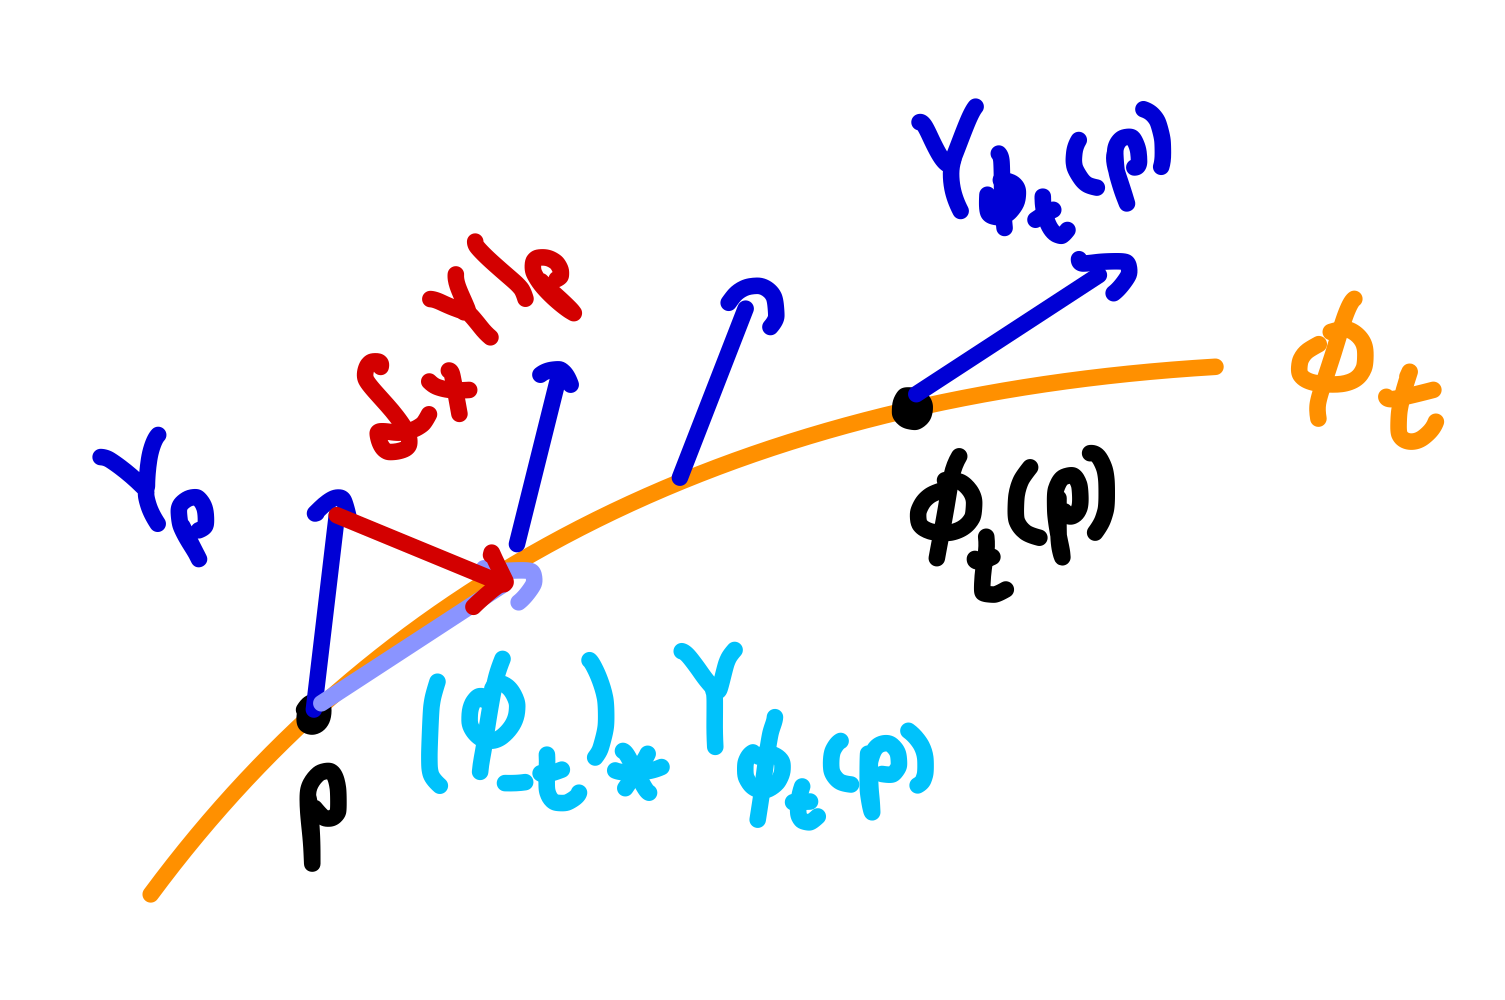
\includegraphics[width=0.4\linewidth]{Bilder/lieabl.png}
\caption{Die Lie-Ableitung eines Vektorfeldes $Y$ in Richtung $X$.}
\end{figure}
\end{definition}
\begin{bemerkung}
Wir wissen, dass $\phi_t \to^{t \to 0} \id_M$ und $\phi_{t\ast} \to^{t \to 0} \id_{TM}$. Deshalb können wir $\Ls_XY|_p$ auch schreiben als 
\begin{equation}
(\Ls_XY)_p = \lim_{t \to 0} \phi_{t\ast} \left( \frac{(\phi_{-t})_\ast Y_{\phi_t(p)} - Y_p}{t}\right) = \lim_{t\to 0} \frac{ Y_{\phi_t(p)} - (\phi_t)_\ast Y_p}{t} \in T_{\phi_t(p)}M.
\end{equation}
\end{bemerkung}
\begin{satz}{Lie-Klammer und Lie-Ableitung}{lieklammerableitung}
Es gilt $\Ls_X Y=[X, Y] (= - L_Y X)$.
\begin{figure}[H]
\label{fig:lieablklammer}
\centering
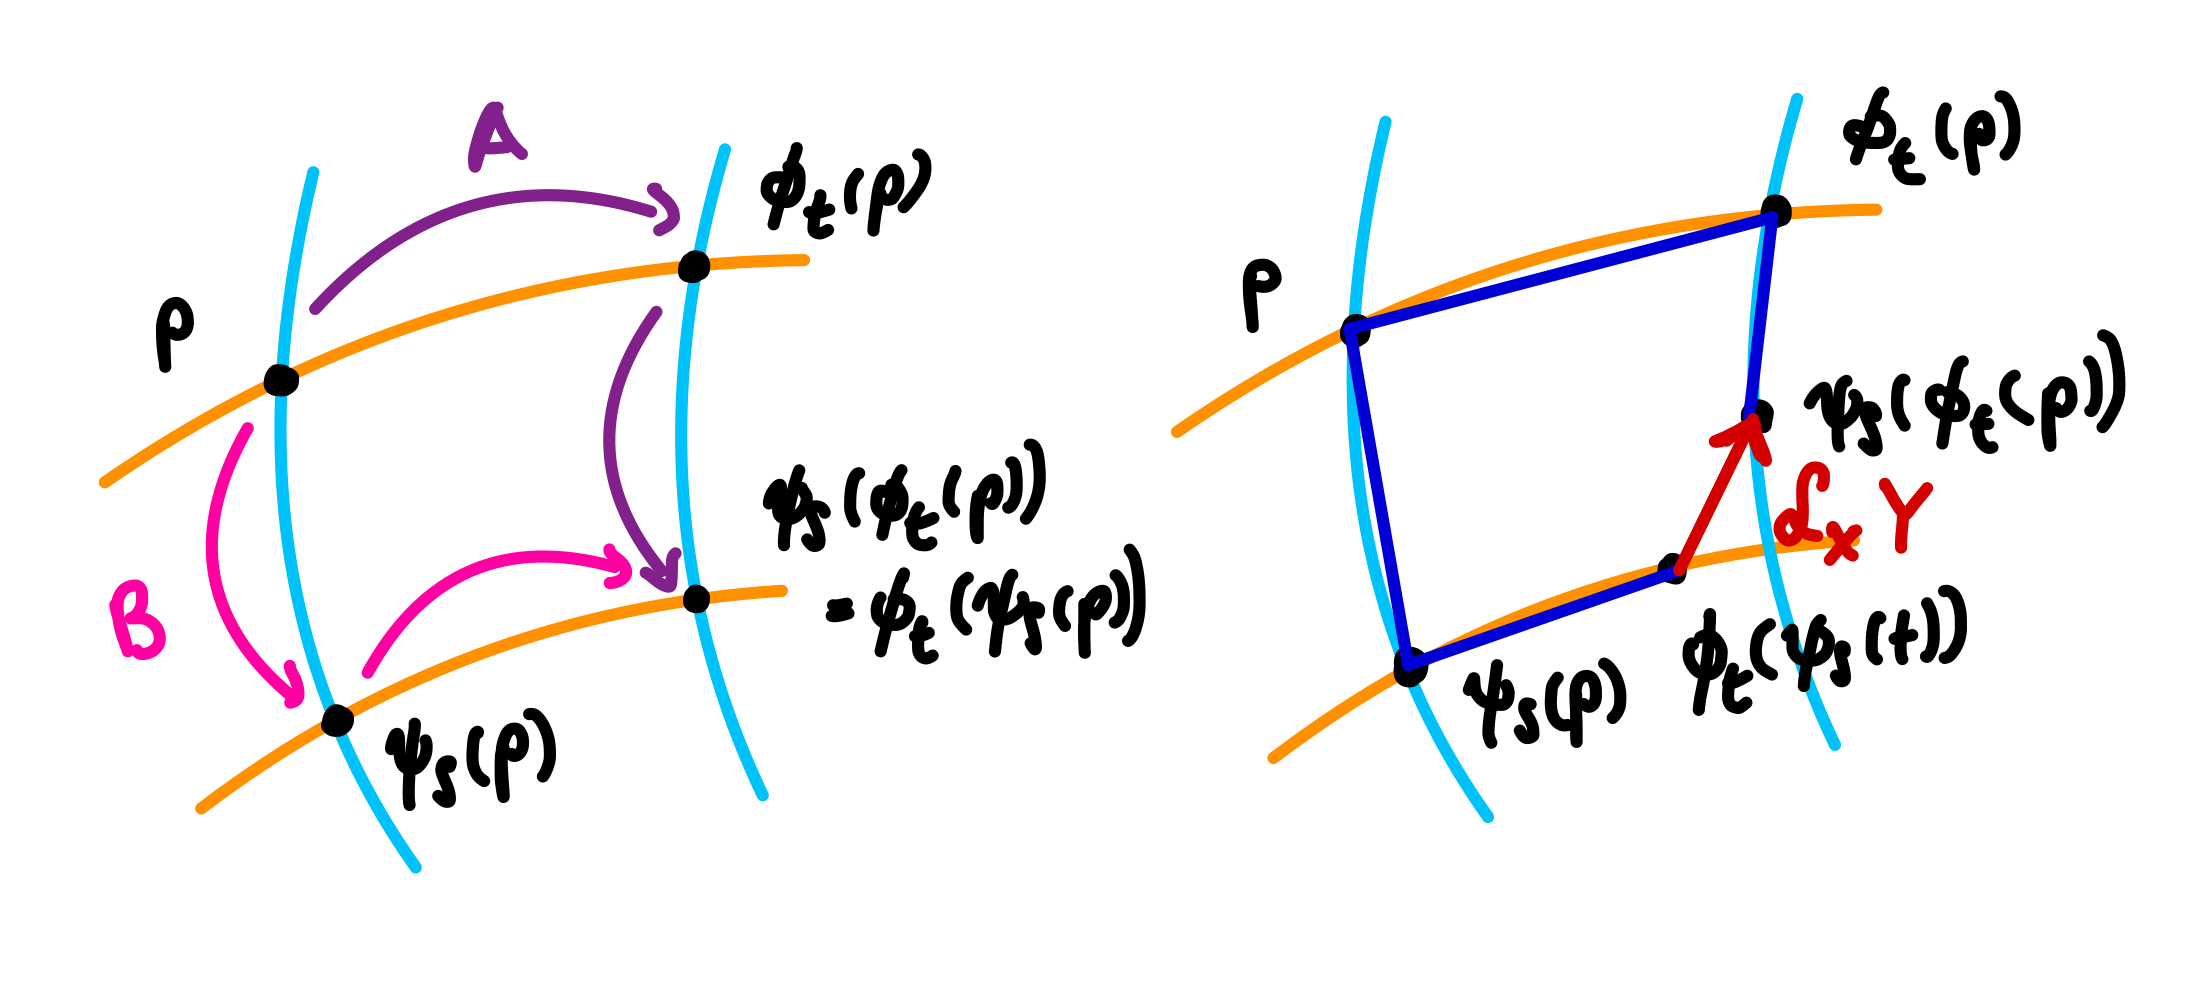
\includegraphics[width=0.4\linewidth]{Bilder/lieablklammer.png}
\caption{Links: Die Lie-Ableitung für Vektorfelder, deren Flüsse kommutieren, verschwindet. Rechts: Die Lie-Ableitung ''ergänzt'' das von den nicht-kommutierenden Flüssen aufgespannte Parallelogramm.}
\end{figure}
\end{satz}
\begin{beweis}
Wir führen den Beweis, indem wir die Wirkung beider Vektorfelder auf eine Funktion $f \in \cinf{M}$ vergleichen. Wir bezeichnen mit $\phi_t$ den Fluss von $X$ und mit $\psi_s$ den Fluss von $Y$. Nun definieren wir für $f\in \cinf{M}$ eine Funktion 
\begin{equation}
A(t):= Y_{\phi_t(p)}(f) = \frac{\partial}{\partial s} f(\psi_s(\phi_t(p)))|_{s=0}.
\end{equation}
und eine Funktion
\begin{equation}
B(t) := (\phi_t)_\ast Y_p(f) = Y_p(f \circ \phi_t) = \frac{\partial}{\partial s} f(\phi_t(\psi_s(p)))|_{s=0}.
\end{equation}
Dann gilt $A(0)=B(0)$ und außerdem 
\begin{align}
(L_XY)_p (f) &= \lim_{t \to 0} \frac{A(t)-B(t)}{t} = \lim_{t \to 0} \frac{A(t) - A(0)}{t} - \lim_{t \to 0} \frac{B(t)-B(0)}{t}\\
&= \frac{\partial^2}{\partial t \partial s} f(\psi_s \phi_t (p))|_{(s, t)=(0,0)} - \underbrace{\frac{\partial^2}{\partial t \partial s}}_{=\frac{\partial^2}{\partial s \partial t}} f(\phi_t \psi_s (p))|_{(s,t)=(0,0)} \\
&= X_p \left( \frac{\partial}{\partial s} (f \circ \psi_s(p))|_{s=0} \right) - Y_p \left( \frac{\partial}{\partial t} (f \circ \phi_t(p))|_{t=0}\right) = X_p(Y(f))- Y_p(X(f)) = [X, Y]_p (f)
\end{align}
\end{beweis}
\begin{korollar}{Aus \ref{lieklammerableitung}}{auslieklammerableitung}
Seien $X, Y \in \Gamma(TM)$ Vektorfelder mit Flüssen $\phi_t$ von $X$ und $\psi_s$ von $Y$. Gilt $[X, Y] =0$, so ist $\phi_t \psi_s = \psi_s \phi_t$ für alle $t,s$, sodass die Ausdrücke für alle $\tau \in [0,t]$ und alle $\sigma \in [0,s]$ definiert sind.
\end{korollar}
\begin{beweis}
$(\Rightarrow)$: Wir wissen, dass $[X,Y]_p(f)=\frac{\partial^2}{\partial t \partial s} f(\psi_s \phi_t (p)))|_{(s,t)=(0,0)} - \frac{\partial^2}{\partial t \partial s} f(\psi_t \phi_s (p)))|_{(s,t)=(0,0)} =0$, da die Flüsse nach Voraussetzung kommutieren.\\
$(\Leftarrow)$: Aus dem vorigen Satz wissen wir, dass 
\begin{equation}
[X, Y]_q = (L_XY)_q = \frac{d}{dt} ((\phi_{-t})_\ast Y_{\phi_t(q)})|_{t=0}.
\end{equation}
Für $t_0 \in I_q$ gilt dann
\begin{equation}
(\phi_{-t_0})_\ast [X,Y]_{\phi_{t_0}(q)} = (\phi_{-t_0})_\ast \left( \frac{d}{dt} (\phi_{-t})_\ast Y_{\phi_t(\phi_{t_0}(q)} \right)|_{t=0} = \frac{d}{d \tau} (\phi_{-\tau})_\ast Y_{\phi_\tau(q)})|_{\tau = t_0}.
\end{equation}
Wenn also $[X,Y]=0$ auf einer Umgebung von $p$, dann ist die Kurve $(-\epsilon, \epsilon) \to T_qM, \ t \mapsto (\phi_{-t})_\ast Y_{\phi_t(q)}$ für alle $q$ nahe $p$ konstant. Also gilt $Y_{\phi_t(q)} = (\phi_t)_\ast Y_q$ für $t$ nahe $0$ und $q$ nahe $p$. Wir betrachten nun die Kurven (für festes $t$) $\gamma_1 = \psi_s(\phi_t (p))$ und $\gamma_2 (s) = \phi_t (\psi_s (p))$. Es gilt: 
\begin{itemize}
\item $\gamma_1(0) = \gamma_2(0) = \phi_t(p)$
\item $\gamma_1$ erfüllt die DGL $\dot{\gamma}_1(s)=Y_{\gamma_1}(s)$.
\item $\gamma_2$ erfüllt diese DGL ebenfalls, denn 
\begin{equation}
\frac{d}{ds} \gamma_2(s) = (\phi_t)_\ast (\frac{d}{ds} \psi_s(p)) = (\phi_t)_\ast Y_{\psi_s(p)} = Y_{\phi_t\psi_s (p)} = Y_{\gamma_2(s)}.
\end{equation}
\end{itemize}
Aus der Eindeutigkeit der Lösung des AWP folgt $\gamma_1 (s) =  \gamma_2(s)$ für alle $s$.
\end{beweis}
\subsection{Liegruppen}
\label{subsec:liegruppen}
\begin{definition}{Lie-Gruppe}{liegruppe}
Eine \textbf{Lie-Gruppe} ist eine Gruppe $G$, sodass die zugrundeliegende Menge $G$ eine glatte MFK ist und die Strukturabbildungen 
\begin{align}
m: G \times G &\to G\\
g,h &\mapsto g \circ h
\end{align}
und
\begin{align}
i: G &\to G\\
g &\mapsto g^{-1}
\end{align}
glatte Abbildungen sind.
\end{definition}
\begin{beispiele}
\begin{enumerate}
\item $(\R^n, +)$: Auch Quotienten bezüglich einer diskreten Untergruppe, z.B. $\T^n = \quotient{\R^n}{\Z^n}$ sind Lie-Gruppen.
\item $\text{GL}(n, \R)$: Multiplikation und Inversenbildung sind glatt.
\item $\text{SL}(n, \R) := \{ A \in \text{GL}(n, \R) | \det (A) =1 \}$: $1$ ist ein regulärer Wert von $\det: \text{Mat}(n,\R) \to \R$, also ist $\text{SL}(n, \R)$ eine Untergruppe und UMF.
\item Mit demselben Argument:
\begin{itemize}
\item $\text{O}(n) := \{ A \in \text{GL}(n, \R) | A^TA = \id \}$.
\item $\text{SO}(n) := \text{O}(n) \cap \text{SL}(n, \R)$
\item $\text{U}(n) := \{ A \in \text{GL}(n, \C) | \bar{A}^TA=\id \} \sub \text{GL}(n, \C) \sub \text{GL}(2n, \R)$. Multiplikation mit $i$, aufgefasst als lineare Abbildung $\R^{2n} \to \R^{2n}$ hat bezüglich der Standardbasis $\R^n \oplus i \R^n$ die Form
\begin{equation}
J_0 = \mat{0, -\id}{\id, 0}.
\end{equation} 
Also gilt $\text{GL}(n, \C) = \{ A \in \text{GL}(2n, \R) | A J_0 = J_0 A\}$.
\item $\text{SU}(n) = \text{U}(n) \cap \text{SL}(2n, \R)$.
\end{itemize}
\item In kleineren Dimensionen trifft man alte Bekannte:
\begin{itemize}
\item $\text{SO}(2) \cong  \sph^1$
\item $\text{SO}(3) \cong \R P^3$ (als MFK)
\item $\text{SU}(2) \cong \sph^3$ (als MFK)
\end{itemize}
\end{enumerate}
\end{beispiele}
\begin{bemerkung}
In jeder Lie-Gruppe $G$ definiert jedes Element $h \in G$ zwei Diffeomorphismen:\\
Linksmultiplikation
\begin{align}
L_h: G &\to G \\
g &\mapsto hg
\end{align}
und Rechtsmultiplikation
\begin{align}
R_h: G &\to G\\
g &\mapsto gh.
\end{align}
Es gilt $R_h = L_h \iff h$ liegt im Zentrum von $G$, also $\forall h \in G: R_h = L_h \iff G$ kommutativ ist.
\end{bemerkung}
\begin{definition}{Linksinvarianz}{linksinvarianz}
Ein Vektorfeld $X \in \Gamma (TG)$ auf einer Lie-Gruppe $G$ heißt \textbf{linksinvariant}, falls $X_{hg} = X_{L_h(g)}=(L_h)_\ast X_g$ für alle $g,h \in G$.
\end{definition}
\begin{bemerkung}
Sei $e \in G$ das neutrale Element der Gruppe. Ist $X$ linksinvariant, so gilt $X_g = X_{L_g(e)} = (L_g)_\ast X_e$. Also sind linksinvariante Vektorfelder eindeutig bestimmt durch ihren Wert in $e \in G$. Umgekehrt definiert diese Formel für jedes $v = X_e \in T_eG$ ein linksinvariantes Vektorfeld, da 
\begin{equation}
X_{gh} = (L_{gh})_\ast X_e = (L_g)_\ast (L_h)_\ast X_e = (L_g)_\ast X_h
\end{equation}
für alle $g, h \in G$ gilt. Also sind linksinvariante Vektorfelder in Bijektion zu $T_eG$.
\end{bemerkung}
\begin{beispiel}
Auf $(\R^n, +)$ sind linksinvariante Vektorfelder translationsinvariante Vektorfelder, d.h. sie haben als Linearkombination der Koordinatenvektorfelder $\frac{\partial}{\partial x_1}, \dots, \frac{\partial}{\partial x_n}$ konstante Koeffizienten.
\end{beispiel}
\begin{lemma}{Linksinvarianz der Lie-Klammer}{linksinvariantelieklammer}
Für linksinvariante Vektorfelder $X,Y$ ist auch $[X, Y]$ linksinvariant.
\end{lemma}
\begin{beweis}
Gemäß Übung (A12) gilt: 
\begin{equation}
[X,Y] = [(L_h)_\ast X, (L_h)_\ast Y]= (L_h)_\ast [X,Y]
\end{equation}
für alle $h \in G$.
\end{beweis}
\begin{korollar}{Lie-Unteralgebra der VF}{lieunteralgebra}
Die linksinvarianten Vektorfelder bilden eine Lie-Unteralgebra in $\Gamma (TG)$.
\end{korollar}
\begin{beweis}
Umformulierung des vorigen Lemmas.
\end{beweis}
\begin{bemerkung}
Indem wir die Identifikation der linksinvarianten Vektorfelder mit dem Tangentialraum $\mathfrak{g}:= T_eG$ vornehmen, erhalten wir eine Lie-Algebra-Struktur:
\begin{align}
[.,.]: \mathfrak{g} \times \mathfrak{g} &\to \mathfrak{g}\\
(\xi, \eta) &\mapsto [X, Y]_e,
\end{align}
wobei $X$ und $Y$ die linksinvarianten Fortsetzungen von $\xi$ und $\eta$ sind.
\end{bemerkung}
\begin{beispiele}
\begin{enumerate}
\item Für $G=(\R^n,+)$ ist die Lie-Klammer auf $\mathfrak{g} \cong \R^n$ trivial, also $[u,v]=0$ für alle $u, v \in \R^n$.
\item Für $G = \text{GL}(n, \R)$ ist $\mathfrak{gl}(n, \R) = \text{Mat}(n, \R)$.
\end{enumerate}
\end{beispiele}
\begin{satz}{Lie-Klammer auf $\mathfrak{gl}(n,\R)$}{lieklammergl}
Die Lie-Klammer auf $\mathfrak{gl}(n, \R)$ hat die Form $[\xi, \eta] = \xi \eta - \eta \xi$.
\end{satz}
\begin{beweis}
Für festes $h \in \text{GL}(n, \R)$ ist die Linksmultiplikation 
\begin{align}
L_h: \text{GL}(n, \R) &\to \text{GL}(n, \R)\\
g &\mapsto hg
\end{align}
linear in $g$, sodass
\begin{equation}
(L_h)_\ast = L_h: \text{Mat}(n,\R) \to \text{Mat}(n, \R).
\end{equation}
Also ist für $\xi \in T_\id \text{GL}(n, \R)$ das zugehörige linksinvariante Vektorfeld $X$, gegeben als $X_g = g \cdot \xi$. Die Gleichung $\dot{g}(t) = X_{g(t)} = \xi g(t)$ hat die eindeutige Lösung $g(t) = g(0) \exp (t \xi)$. Der Fluss $\phi_t$ von $X$ hat also die Form $\phi_t (g) = g \exp (t \xi)$. Wie zuvor gilt $(\phi_t)_\ast = R_{\exp (t \xi)}$. Sind nun $\xi, \eta \in T_\id \text{GL}(n, \R)$ mit zugehörigen linksinvarianten Vektorfeldern $X$ und $Y$, so gilt
\begin{equation}
[\xi, \eta] = [X,Y]_\id = (\Ls_XY)_\id = \left.\frac{d}{dt} \left( (\phi_t)_\ast Y_{\phi_t(\id)} \right)\right|_{t=0}=\left. \frac{d}{dt} \exp(t \xi) \eta \exp(-t \xi) \right|_{t=0} = \xi \eta- \eta \xi.
\end{equation}
\end{beweis}
\begin{figure}[H]
\label{fig:linksinvariant}
\centering
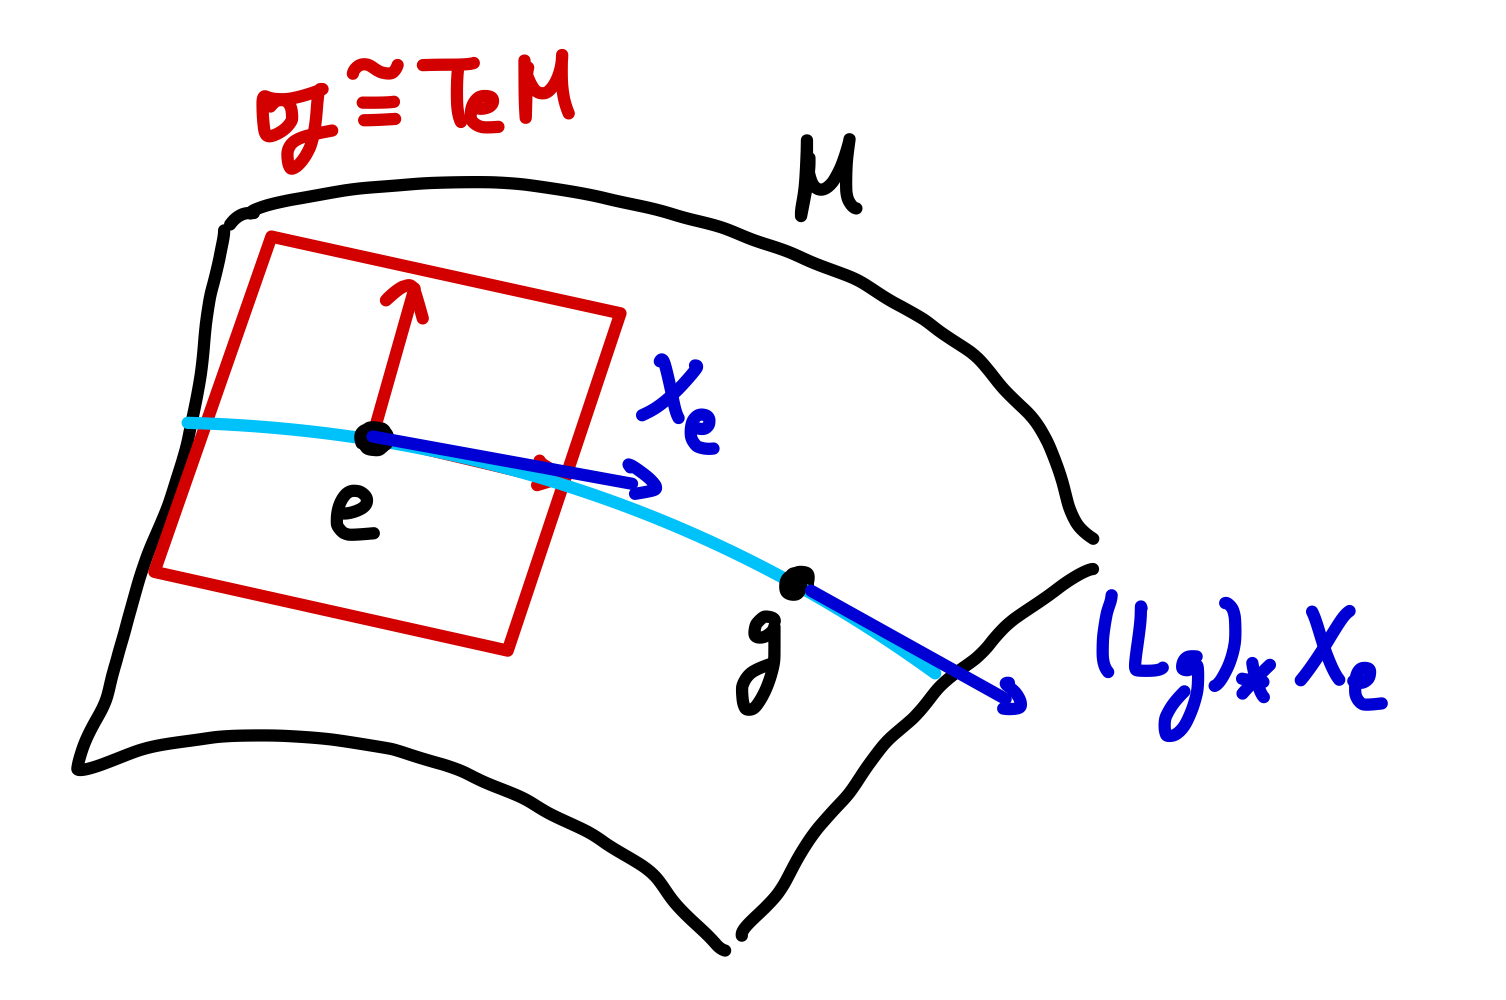
\includegraphics[width=0.3\linewidth]{Bilder/linksinvariant.png}
\caption{Eine Lie-Gruppe als Tangentialraum an der Identität mit linksinvariantem Vektorfeld.}
\end{figure}
\begin{bemerkung}
Die Rechnung zeigt: Linksinvariante Vektorfelder auf $\text{GL}(n, \R)$ sind vollständig. Das gilt allgemein für alle Lie-Gruppen: Ist $X \in \Gamma (TG)$ linksinvariant und $\gamma: I_e \to G$ die maximale Integralkurve durch $e \in G$, dann ist $L_g \circ \gamma: I_e \to G$ eine Integralkurve durch $g$
\begin{equation}
\frac{d}{dt}(L_g \circ \gamma) = (L_g)_\ast \dot{\gamma} = (L_g)_\ast X = X.
\end{equation}
Für $g = \gamma(t)$ mit $t \neq 0$ wissen wir, dass $I_g = I_e -t$, also geht $I_e \sub I_g$ für alle $g = \gamma (t)$ nur für $I_e = \R$.
\end{bemerkung}
\begin{definition}{Exponentialabbildung}{expabb}
Sei $G$ eine Lie-Gruppe. Die \textbf{Exponentialabbildung}
\begin{equation}
\exp: T_eG = \mathfrak{g} \to G
\end{equation}
ist definiert als $\exp (\xi) = \gamma_\xi (1)$, wobei $\gamma_\xi: \R \to G$ die Integralkurve des zu $\xi$ gehörenden, linksinvarianten Vektorfeldes mit $\gamma_\xi (0)=e$ ist.
\end{definition}
\begin{bemerkung}
Der Name Exponentialabbildung kommt daher, dass für Matrixgruppen $\exp(\xi) = e^\xi$ gilt.
\end{bemerkung}
\begin{beispiel}
Für $G = \quotient{\R^n}{\Z^n} \cong T^n$ ist die Exponentialabbildung $exp: \R^n \to \quotient{\R^n}{\Z^n}$ die universelle Überlagerung von $T^n$, d.h. die Abbildung, die $x\in \R^n$ auf seine Äquivalenzklasse $[x] \in T^n$ abbildet.
\end{beispiel}
\begin{satz}{Differential als Gruppenhomomorphismus}{diffhomo}
Ist $\phi: G \to H$ ein glatter Gruppenhomomorphismus, dann ist $\phi_{\ast, e}: \mathfrak{g} \to \mathfrak{h}$ ein Homomorphismus von Lie-Algebren.
\end{satz}
\begin{beweis}
Wir müssen zeigen, dass $\phi_\ast [\xi, \eta] = [\phi_\ast \xi, \phi_\ast \eta]$.\\
Dafür wollen wir ÜA (A12) nutzen. Um das dort gezeigte Ergebnis anwenden zu können, müssen wir zeigen, dass für die linksinvarianten Vektorfelder $X,Y$ auf $G$ zu $\xi, \eta$ bzw. $\overline{X}, \overline{Y}$ auf $H$ zu $\phi_\ast \xi, \phi_\ast \eta$ die Gleichung $\phi_\ast (X_g) = \overline{X}_{\phi(g)}$ und analog für $\overline{X}, \overline{Y}$ gilt.\\
$\phi$ ist ein Gruppenhomomorphismus, sodass gilt:
\begin{align}
\phi(gh) &= \phi(g) \phi(h) \\
\phi \circ L_g &= L_{\phi(g)} \phi \\
\implies \phi_\ast L_{g_\ast} &= L_{\phi (g)\ast} \phi_\ast\\
\iff \phi_\ast &= L_{\phi (g), \ast} \phi_\ast \underbrace{(L_{g \ast})^{-1}}_{(L_{g^{-1}})_\ast}.
\end{align}
Daraus folgt, dass
\begin{align}
\phi_\ast X_g &= L_{\phi(g)\ast} \phi_\ast (L_{g^{-1}})_\ast X_g\\
&= L_{\phi(g)\ast} \phi_\ast \xi \\
&= \overline{X}_{\phi(g)},
\end{align}
was zu zeigen war.
\end{beweis}
\begin{beispiel}
Wir betrachten den Gruppenhomomorphismus 
\begin{equation}
\det: GL(n, \R) \to \R^\ast = (\R \exc \{0\}, \cdot).
\end{equation}
Wir zeigen, dass $det_{\ast, \id} = \Tr: \text{Mat}(n, \R) \to \R$ gilt.\\
Seien $A \in \text{GL}(n, \R)$ und $\xi \in \text{Mat}(n, \R)$ mit Spaltenvektoren $a_1, \dots, a_n$ und $\xi_1, \dots, \xi_n$. Dann gilt 
\begin{equation}
\frac{d}{dt} \det (A+t \xi)|_{t=0} = \Sum{i,1,n} \det (a_1, \dots, a_{i-1}, \xi_i, a_{i+1}, \dots, a_n).
\end{equation}
Für $A = \id \in \text{GL}(n, \R)$ gilt dann
\begin{align}
\frac{d}{dt} \det (\id + t \xi)|_{t=0} &= (\det)_{\ast, \id}(\xi) \\
&= \Sum{i,1,n} \det \mat{1, 0, \cdots,0, \xi_{1i}, 0,0, \cdots, 0}{0, 1, \cdots,0, \xi_{2i}, 0,0, \cdots, 0}{\vdots, \vdots,  \ddots,\vdots, \vdots, \vdots,\vdots, \ddots, \vdots}{0,0,\cdots,1,\xi_{(l-1)i},0,0,\cdots,0}{0, 0, \cdots,0, \xi_{li}, 1,0, \cdots, 0}{0, 0, \cdots,0, \xi_{(l+1)i}, 0,1, \cdots, 0}{\vdots,\vdots, \ddots,\vdots, \vdots, \vdots, \vdots, \ddots, 0}{0,0, \cdots, 0, \xi_{ni}, 0,0,\cdots,1}\\
&= \Sum{i,1,n} \xi_{ii} = \Tr \xi.
\end{align}
\end{beispiel}
Auf $\R$ verschwindet die Lie-Klammer. Auf $\text{Mat}(n, \R)=\mathfrak{gl}(n, \R)$ gilt aber $[\xi, \eta] = \xi \eta - \eta \xi$. Der Satz sagt dann $\Tr(\xi \eta - \eta \xi)=\Tr (\xi \eta) - \Tr (\eta \xi)=0$. Wir erhalten also die bekannte Aussage $\Tr (\xi \eta) = \Tr (\eta \xi)$ für alle $\xi, \eta \in \mathfrak{gl}(n, \R)$.
\begin{bemerkungen}
Zwei wichtige Sätze von \emph{Lie} sagen:
\begin{enumerate}
\item Zu jeder endlich-dimensionalen Lie-Algebra $\mathfrak{g}$ existiert eine bis auf Isomorphie eindeutige, einfach-zusammenhängende Lie-Gruppe $G$ mit $T_eG=\mathfrak{g}$.
\item Ist $\overline{\phi}: \mathfrak{g} \to \mathfrak{h}$ eine Homomorphismus zwischen endlich-dimensionalen Lie-Algebren, so existiert für \textit{jede} Lie-Gruppe $H$ mit Lie-Algebra $\mathfrak{h}$ ein Gruppenhomomorphismus $\phi: G \to H$ von der einfach-zusammenhängenden Lie-Gruppe $G$ mit Lie-Algebra $\mathfrak{g}$ mit $\phi_{\ast, e} = \overline{\phi}$.
\end{enumerate}
\end{bemerkungen}
\begin{beispiel}
Hat die Lie-Algebra $\mathfrak{h}$ der Lie-Gruppe $H$ eine abelsche Lie-Unteralgebra $\mathfrak{h}_0 \sub \mathfrak{h}$, dann existiert eine abelsche Lie-Untergruppe $H_0 \sub H$ mit $T_eH_0 = \mathfrak{h}$.
\end{beispiel}
\subsection{Differentialformen auf Mannigfaltigkeiten}
\label{subsec:diffformen}
Die Theorie funktioniert ganz analog zum Fall von UMF des $\R^n$.
\begin{satz}{1-Formen als lokaler Rahmen}{formenlokrahmen}
Sei $Q$ eine glatte MFK, $TQ$ das Tangentialbündel und $T^\ast Q$ das Kotangentialbündel. Sind $(q_1, \dots, q_n)$ lokale Koordinaten auf $U \sub Q$, so sind die $1$-Formen $dq_1, \dots, dq_n$ ein lokaler Rahmen für $T^\ast Q|_M$.
\end{satz}
Jeder Punkt in $T^\ast Q|_M$ lässt sich also schreiben als $(q, \alpha_q)$ mit $q \in U$ und $\alpha_q \in T^\ast_q Q = \text{L}(T_q Q, \R)$. Dabei hat $\alpha_q$ eine eindeutige Darstellung als $\alpha_q = \Sum{j,1,n} p_j (d_{q_j})_q$ mit $p_j \in \R$.
\begin{bemerkung}Kanonische Koordinaten\\
$(q_1, \dots, q_n, p_1, \dots, p_n)$ bilden lokale Koordinaten auf $T^\ast Q|_U$. Man nennt diese Koordinaten auch die \textbf{kanonischen Koordinaten} auf $T^\ast Q|_U$ assoziiert zu den Koordinaten $(q_1, \dots, q_n)$ auf $U$.
\end{bemerkung}
\begin{satz}{Globale $1$-Form}{globdiff}
Durch $\lambda := \Sum{j,1,n} p_j dq_j$ wird eine $1$-Form auf $T^\ast Q|_U$ definiert. Diese in lokalen, kanonischen Koordinaten definierten $1$-Formen auf $T^\ast Q$ passen zusammen zu einer global definierten $1$-Form $\lambda_{\text{can}}$ auf $M = T^\ast Q$. Eine beliebige glatte $1$-Form $\alpha \in \Omega^1(Q)$ ist ein Schnitt in $T^\ast Q$, also eine Abbildung 
\begin{equation}
\alpha: Q \to T^\ast Q
\end{equation}
mit $\pi_\alpha = \id$.
\end{satz}
\begin{satz}{Pullback einer Differentialform}{pullbackdiff}
Für alle $\alpha \in \Omega^1 (Q)$ gilt $\alpha^\ast (\lambda_{\text{can}}) = \alpha$.
\end{satz}
\begin{bemerkung}
Es gilt $d\lambda_\text{can} \in \Omega^2(T^\ast Q)$. In lokalen, kanonischen Koordinaten gilt
\begin{equation}
d \lambda_\text{can} = \Sum{j,1,n} dp_j \wedge dq_j.
\end{equation}
Diese Form ist nicht-ausgeartet in dem Sinn, dass $T(T^\ast Q) \to T_x^\ast(T^\ast Q), \ v \mapsto i_v d \lambda_\text{can}$ ein Isomorphismus ist.\\
$(T^\ast Q, d \lambda_\text{can})$ ist ein Beispiel für eine \textit{symplektische MFK}.
\end{bemerkung}
\begin{definition}{Symplektische MFK}{symplek}
Ein Paar $(M, \omega)$ heißt \textbf{symplektische MFK}, wenn $\omega \in \Omega^2 (M)$ und $d\omega = 0$ gilt und $\omega$ nicht ausgeartet ist, d.h., dass $\forall p \in M$ 
\begin{align}
T_pM &\to T_p^\ast M \\
v &\mapsto \omega(v, .)
\end{align}
ein Isomorphismus ist.
\end{definition}
\begin{definition}{\textit{Hamiltonsches Vektorfeld}}{hamilton}
Sei $H: T^\ast \R^n \to \R$ eine glatte Funktion und $\omega = \omega_\text{can} \in \Omega^2(T^\ast \R^n)$ die kanonische symplektische Form. Dann definiert die Gleichung
\begin{equation}
X \iprod \omega = -dH
\end{equation}
das zu $H$ gehörige \textbf{Hamiltonsche Vektorfeld}.
\end{definition}
\begin{satz}{Invarianz unter $X$}{invarianz}
Sei $X$ das Hamiltonsche Vektorfeld der glatten Abbildung $H: T^\ast \R^n \to \R$ und $\omega_\text{can}$ die kanonische symplektische Form. Dann gilt für den Fluss $\phi_t: T^\ast \R^n \to \T^\ast \R^n$, dass 
\begin{equation}
\phi_t^\ast \omega = \omega,
\end{equation}
also ist $\omega$ invariant unter dem Fluss von $X$. Insbesondere ist die Volumenform $\mu:= \omega^{\wedge n} \in \Omega^{2n}(T^\ast \R^n)$ invariant unter $\phi_t$.
\end{satz}
\begin{beweis}
Übung 6.3
\end{beweis}
\begin{definition}{$k$-Formen}{kforms}
Glatte $k$\textbf{-Formen} auf $Q$ sind Schnitte in einem Bündel $\Lambda^k T^\ast Q \to Q$.
\end{definition}
Sind $q_1, \dots, q_n$ lokale Koordinaten auf $Q$, so bilden die Formen
\begin{equation}
dq^I := dq_{i_1} \wedge \cdots \wedge dq_{i_k}
\end{equation}
mit $\{ i_1 < \cdots < i_k \} =: I$ einen lokalen Rahmen für $\Lambda^k T^\ast Q$, d.h. jede glatte $k$-Form kann lokal geschrieben werden als
\begin{equation}
\eta|_U = \sum_{I = \{i_1 < \cdots  < i_k \}} \eta_I dq^I
\end{equation}
mit $\eta_I \in \cinf{U}$.
\begin{definition}{Äußeres Differential}{outerdiff}
Das \textbf{äußere Differential} $d: \Omega^k (Q) \to \Omega^{k+1} (Q)$ ist charakterisiert durch folgende Eigenschaften:
\begin{itemize}
\item Für Funktionen $f: Q \to \R$ gilt $df = f^\ast dt$, wobei $dt$ die Standard-$1$-Form auf $\R$ ist. Insbesondere gilt dann $df(X) = X(f)$.
\item $d(\eta_1 \wedge \eta_2) = (d \eta_1) \wedge \eta_2 + (-1)^{\text{deg} \ \eta_1} \eta_1 \wedge d \eta_2$.
\item $d^2 = 0$.
\end{itemize}
\end{definition}
\begin{definition}{\textit{Lie-Ableitung für Differentialformen}}{liedifferential}
Sei $M$ eine glatte MFK, $X \in \Gamma(TM)$ ein glattes Vektorfeld und $\omega \in \Omega^k(M)$ eine $k$-Form. Dann definiert
\begin{equation}
\Ls_x \omega := \lim_{t \to 0} \frac{\phi_t^\ast \omega - \omega}{t}
\end{equation}
die \textbf{Lie-Ableitungen für Differentialformen}, wobei $\phi_t$ der Fluss von $X$ ist.
\end{definition}
\begin{definition}{\textit{Inneres Produkt}}{inneresdifferential}
Sei $M$ eine glatte MFK und $X \in \Gamma(TM)$ ein glattes Vektorfeld. Dann ist das \textbf{innere Produkt} die lineare Abbildung
\begin{align}
\iprod: \Omega^k(M) &\to \Omega^{k-1}(M)\\
\omega &\mapsto X \iprod \omega(X_1, \dots, X_{k-1}) = \omega(X, X_1, \dots, X_{k-1}.
\end{align}
Man schreibt auch $X \iprod \omega = i_X \omega$.
\end{definition}
\begin{bemerkung}
Es gelten meherere Formeln für das innere Produkt, die in (A15) und (A16) bewiesen werden:
\begin{itemize}
\item Für alle $X \in \Gamma(TM)$ glatt, $\omega_1 \in \Omega^k(M)$ und $\omega_2 \in \Omega^l(M)$ gilt 
\begin{equation}
X \iprod (\omega_1 \wedge \omega_2) = (X \iprod \omega_1) \wedge \omega_2 + (-1)^k \omega_1 \wedge (X \iprod \omega_2).
\end{equation}
\item Sei $\eta \in \Omega^1(M)$ und $X,Y \in \Gamma(TM)$ glatt. Dann gilt
\begin{equation}
d\eta(X,Y) = X(\eta(Y))-Y(\eta(X))-\eta([X,Y]).
\end{equation}
\end{itemize}
\end{bemerkung}
\begin{theorem}{\textit{Cartans magische Formel}}{cartansmagie}
Sei $M$ eine glatte MFK, $X \in \Gamma(TM)$ glatt und $\omega \in \Omega^k(M)$ eine glatte $k$-Form. Dann gilt
\begin{equation}
\Ls_X \omega = d(X \iprod \omega) + X \iprod d\omega.
\end{equation}
\end{theorem}
Um über Integration zu reden, benötigen wir Orientierungen:
\begin{definition}{Orientierbarkeit}{orientierung}
$Q$ heißt \textbf{orientierbar}, falls es einen Atlas $\mathfrak{A} = \{ (U_\alpha, \phi_\alpha) \}_{\alpha \in I}$ gibt, sodass alle Übergangsabbildungen $\phi_{\alpha \beta}$ orientierungserhaltende Diffeomorphismen von offenen Teilmengen des $\R^n$ sind, d.h. die Ableitungen $\Ds \phi_{\alpha \beta}$ haben überall positive Determinante.\\
Eine \textbf{Orientierung} auf $Q$ sit eine Wahl eines solchen orientierten Atlasses.
\end{definition}
\begin{bemerkungen}
\begin{enumerate}
\item Ist $Q$ zusammenhängend und orientierbar, so gibt es genau zwei mögliche Orientierungen auf $Q$.
\item $Q$ ist orientierbar. $\iff$ Es existiert eine globale Volumenform $\omega \in \Omega^{\dim Q} (Q)$ mit $\omega_q \neq 0$ für alle $q \in Q$. Jede solche Volumenform gibt uns eine Trivialisierung $\Lambda^{\dim Q} T^\ast Q \cong \underline{\R} = Q \times \R$ und umgekehrt.
\end{enumerate}
\end{bemerkungen}
\begin{satz}{Zerlegung der Eins}{zerlegungeins}
Sei $Q$ eine glatte MFK und $\mathfrak{A} = \{ (U_\alpha, \phi_\alpha) \}_{\alpha \in I}$ ein Atlas. Dann existiert eine diesem Atlas untergeordnete Zerlegung der Eins, d.h. eine Familie von glatten Funktionen $\{ \rho_\alpha: Q \to \R \}_{\alpha \in I}$ mit folgenden Eigenschaften:
\begin{itemize}
\item $\supp \rho_\alpha \sub U_\alpha$
\item $0 \leq \rho_\alpha \leq 1$
\item Zu jedem $q \in Q$ existiert eine offene Umgebung $U \sub Q$, sodass $\supp \rho_\alpha \cap U \neq \emptyset$ für endlich viele $\alpha \in I$.
\item $\sum_{\alpha \in I} \rho_\alpha \equiv 1$.
\end{itemize}
\end{satz}
Ist $\Omega^n_0 (Q) \sub \Omega^n (Q)$ der Raum der $n$-Formen mit kompaktem Träger, so gibt Integration eine $\R$-lineare Abbildung:
\begin{equation}
\int : \Omega_0^n (Q) \to \R.
\end{equation}
Wir wollen uns allgemein MFKn mit Rand zuwenden. Für top. MFK forderten wir die Hausdorffeigenschaft, eine abzählbare Basis und, dass jeder Punkt eine Umgebung besitzt, die homöomorph zu $U \sub \R^n$ offen ist. Die letzte Eigenschaft wollen wir ersetzen:
\begin{definition}{Top. MFK mit Rand}{randmfk}
Sei $X$ hausdorffsch und habe eine abzählbare Basis. Jeder Punkt $p \in X$ habe eine Umgebung, die homöomorph zu einer im Halbraum 
\begin{equation}
\R_-^n := \{ x=(x_1, \dots, x_n) \in \R^n \ | \ x_1 \leq 0\}
\end{equation}
liegenden offenen Teilmenge ist. Dann heißt $X$ \textbf{berandete (top.) Mannigfaltigkeit}.
\end{definition}
\begin{definition}{Randpunkte}{randpunkte}
\textbf{Randpunkte} von $X$ sind Punkte, die für einen (und daher für jeden solchen) Homöomorphismus nach $\{0\} \times \R^{n-1}$ abgebildet werden.
\end{definition}
\begin{definition}{Rand}{rand}
Sei $X$ eine berandete MFK. Dann ist der \textbf{Rand} $\partial X$ eine top. MFK ohne Rand.
\end{definition}
\begin{definition}{Glatte Funktionen}{glattefn}
Seien $U, V \sub \R^n_-$ offen. Eine Abbildung $f: U \to V$ nennen wir \textbf{differenzierbar}, \textbf{glatt} oder \textbf{von Klasse} $C^k$, falls offene Teilmengen $\tilde{U}, \tilde{V} \sub \R^n$ und eine diffbare/glatte/$C^k$-Abbildung $\tilde{f}: \tilde{U} \to \tilde{V}$ existiert, sodass $\tilde{f}|_U = f$.
\end{definition}
\begin{definition}{Glatte berandete MFK}{glattrand}
Sei $X$ eine berandete MFK. $X$ heißt \textbf{glatt}, wenn ein Atlas existiert, in dem alle Kartenübergänge Diffeomorphismen von offenen Teilmengen in $\R_-^n$ in diesem Sinne sind.
\end{definition}
Ist $p \in \partial X$, dann ist $T_p \partial X \sub T_p X$ ein UR der Kodimension $1$. Ein nach außen gerichteter Vektor in $T_pX$ ist ein $v \in T_pX$, der unter dem Differential einer Kartenabbildung $\phi: U \to \R_-^n$ auf einen Vektor mit positiver Komponente in Richtung $\frac{\partial}{\partial x_1}$ abgebildet wird. Ist $X$ orientiert, so induziert diese Orientierung auch eine Orientierung auf $\partial X$: $(v_2, \dots, v_n) \in T_p \partial X$ ist genau dann positiv orientiert, wenn für einen nach außen gerichteten Vektor $v \in T_pX, (v, v_2, \dots, v_n)$ eine positive Basis von $T_pX$ ist. 

\begin{theorem}{Satz von Stokes}{stokes}
Sei $Q$ eine berandete MFK mit Rand $\partial Q = P$ und $\dim P = n$. Sei $Q$ außerdem orientiert.\\
Für $\eta \in \Omega_0^n (Q)$ gilt dann
\begin{equation}
\int_Q d \eta = \int_P \eta.
\end{equation}
\end{theorem}


\begin{definition}{Geometrische Distribution}{geomdist}
Sei $M$ eine glatte MFK der Dimension $n$. In jedem Tangentialraum sei ein $k$-dim. UR $D_p \sub T_p M$, der glatt vom Punkt $p \in M$ abhängt (d.h. $D \sub TM$ ist ein $k$-dim. Unterbündel: Es existieren lokale Trivialisierungen von $TM$, sodass $D|_U$ gerade von den ersten $k$ Schnitten des lokalen Rahmens aufgespannt wird.). Man nennt $D$ auch \textbf{(geometrische) Distribution} der Dimension $k$.\footnote{Dies hat nichts mit den Distributionen der Analysis zu tun.}
\end{definition}
Wir stellen uns nun die Frage, unter welchen Bedingungen an $D$ durch jeden Punkt $p \in M$ eine $k$-dim UMF $B_p \sub M$ existiert, die in allen Punkten tangential zu $D$ ist.
\begin{beispiel}
Im Fall $k=1$ finden wir lokal stets ein Vektorfeld $V$, sodass $D = \spn V$. Die Integralkurve des Vektorfeldes, d.h, die Lösungen von $\dot{\gamma}(t) = V_{\gamma (t)}$ sind die Lösungen des in der Frage formulierten Problems.
\end{beispiel}
\begin{bemerkung}
Lokal ist eine $k$-dim. Distribution stets gegeben als gemeinsame Nullstellenmenge von $(n-k)$ glatten $1$-Formen. Konkret ist für $k=n-1$ eine Distribution lokal als Kern \textit{einer} 1-Form gegeben.
\end{bemerkung}
\begin{beispiel}
Auf $\R^3$ betrachten wir die Form $\alpha = dz +y dx$. Für die Distribution $D = \ker \alpha$ existiert überhaupt keine Integral-UMF. Wäre $B \sub \R^3$ eine Integralfläche für $D$, so könnten wir $B$ lokal beschreiben als Bild einer Immersion
\begin{equation}
h: U \to \R^3
\end{equation}
mit $U \sub \R^3$ offen. Seien $h_1, h_2$ und $h_3$ die Komponenten von $h$. Dann gilt $h^\ast \alpha = dh_3 + h_2 dh_1$. $B$ ist tangential an $D$ heißt, dass $h^\ast \alpha \equiv 0$. Daraus folgt $0 = dh_1 \wedge h^\ast \alpha = dh_1 \wedge dh_3$. Dann verschwindet auch das äußere Differential, also $0 = - d(h^\ast \alpha) = dh_1 \wedge dh_2$. Daraus folgt 
\begin{equation}
0 = dh_2 \wedge h^\ast \alpha = dh_2 \wedge dh_3 + h_2 \cancel{dh_2 \wedge dh_1} = dh_2 \wedge dh_3
\end{equation}
Also sind $dh_1, dh_2$ und $dh_3$ in jedem Punkt paarweise linear abhängig. Also kann der Rang von $\Ds h$ nicht größer als $1$ sein. Das ist ein Widerspruch zur Annahme, dass $h$ eine Immersion ist.
\end{beispiel}
Interessant ist, was in diesem Beispiel schiefgeht. Wäre $B$ eine Integralfläche für $D$, so müsste die Lie-Klammer von Vektorfeldern, die tangential an $B$ sind, auch wieder tangential an $B$ sein (Übung A12). Aber $D$ wird aufgespannt durch $X = \frac{\partial}{\partial x} - y \frac{\partial}{\partial z}$ und $Y = \frac{\partial}{\partial y}$. Es gilt jedoch $[X,Y] = \frac{\partial}{\partial z} \notin \ker \alpha$.
\begin{theorem}{Satz von Frobenius}{frobenius}
Sei $M$ eine glatte MFK und $D \sub TM$ eine glatte Distribution von Rang $k$. Dann sind folgende Aussagen äquivalent:
\begin{enumerate}
\item $D$ ist \textbf{integrabel}, d.h. durch jeden Punkt $p \in M$ existiert eine Integral-MFK der Dimension $k$ für $D$.
\item $D$ ist \textbf{involutiv}, d.h. für beliebige Vektorfelder $X, Y \in \Gamma (D)$ gilt $[X, Y] \in \Gamma (D)$.
\item Ist $U \sub M$ offen und $D = \ker \alpha_1 \cap \cdots \cap \ker \alpha_{n-k}$ für punktweise linear unabhängige $1$-Formen $\alpha_1, \dots, \alpha_{n-k} \in \Omega^1(U)$. Dann gilt für jedes $1 \leq j \leq n-k$
\begin{equation}
(d \alpha_j)\wedge \alpha_1 \wedge \cdots \wedge \alpha_{n-k} = 0.
\end{equation}
\item Sind $U$ und $\alpha_1, \dots, \alpha_{n-k}$ wie in $3.$, so existieren $1$-Formen $\theta_{ij} \in \Omega^1 (U)$ mit $1 \leq i$, $j \leq n-k$, sodass
\begin{equation}
d \alpha_j = \Sum{i, 1, n-k} \theta_{ij} \wedge \alpha_i
\end{equation}
für alle $1 \leq j \leq n-k$.
\end{enumerate}
\end{theorem}
\begin{korollar}{Spezialfall von Frobenius}{spezfrob}
$k=1$: Hier ist die Form $(d \alpha_j) \wedge \alpha_1 \wedge \cdots \wedge \alpha_{n-1}$ eine $n+1$-Form auf $M$, also trivialerweise $0$.\\
$k=n-1$: Hier hat die Integrabilitätsbedingung $3.$ dann die Form $d\alpha \wedge \alpha = 0$.
\end{korollar}
\begin{beweis}
Der Beweis lässt sich im Buch von Agricola und Friedrich finden.\\
Allgemein einfach sind $2. \iff 3. \iff 4.$ und $1. \implies 3.$. Kompliziert ist $3. \implies 1.$.\\
$4. \implies 3.$ ist trivial, da $\alpha \wedge \alpha = 0$ für alle $\alpha \in \Omega^1(M)$.\\
$3. \implies 4.$: Wir ergänzen die Form $\alpha_1, \dots, \alpha_{n-k}$ durch geeignete Formen $\beta_1, \dots, \beta_n$ zu einem lokalen Rahmen von $T^\ast M|_U$. Dann gilt
\begin{equation}
d\alpha_j = \sum_{r < s} A_{rs} \alpha_{r} \wedge \alpha_s + \sum_{r,l} B_{rl} \alpha_r \wedge \beta_l + \sum_{l < m} C_{lm} \beta_l \wedge \beta_m.
\end{equation}
$3.$ ist nun äquivalent dazu, dass $\sum_{l < m} C_{lm} (\beta_l \wedge \beta_m) \wedge \alpha_1 \wedge \cdots \wedge \alpha_{n-k} = 0$, woraus $C_{lm} = 0$ für alle $l < m$ folgt. Aus den ersten beiden Termen kann man jeweis $\alpha_r$ ausklammern und erhält so $\theta_{jr}$ mit 
\begin{equation}
d \alpha_j = \Sum{r, i, n-k} \theta_{jr} \wedge \alpha_r.
\end{equation}
$2. \implies 3.$: $\eta_j = (d \alpha_j) \wedge \alpha_1 \wedge \cdots \wedge \alpha_{n-k}$ ist eine $n-k+2$-Form. Setzen wir $(n-k+2)$ Vektorfelder in $\eta_j$ ein, so können wir o.B.d.A. annehmen, dass mindestens zwei davon tangential an $D$ sind. Seien $V, W$ diese beiden Vektorfelder. Für die einzigen potentiell nicht verschwindenden Terme müssen $V$ und $W$ beide in $d \alpha_j$ eingesetzt werden. Aber 
\begin{equation}
d \alpha_j (V,W) = \cancel{V( \alpha_j (W))} - \cancel{W(\alpha_j (V))} - \alpha_j ([V,W]).
\end{equation}
$3. \implies 2.$ Voriges Argument rückwärts lesen.
\end{beweis}
\begin{bemerkung}
Für Hyperebenenfelder $D^{n-1} \sub TM$ mit $D = \ker \alpha$ ist die Integrabilitätsbedingung $\alpha \wedge d\alpha = 0$. Hat $M$ die Dimension $2d+1$, existieren (zumindest lokal) $1$-Formen, die \textit{maximal nicht-integrabel} sind, in dem Sinne, dass $\alpha \wedge (d\alpha)^{\wedge d}$ nirgends verschwindet, also eine (lokale) Volumenform ist.
\end{bemerkung}
Dies liefert eine Definition.
\begin{definition}{Kontaktmannigfaltigkeit}{kontaktmfk}
Eine \textbf{Kontaktmannigfaltigkeit} ist eine MFK $M^{2d+1}$ mit einem maximal nicht-integrablen Hyperebenenfeld $\xi^{2d} \sub TM$.
\end{definition}
\begin{beispiel}
Auf $\R^{2d+1}$ mit Koordinaten $(x_1, \dots, x_d, y_1, \dots, y_d, z)$ erfüllt
\begin{equation}
\xi = \ker \left(\alpha = dz + \Sum{i,1,d} y_i dx_i \right)
\end{equation}
diese Bedingung.
\end{beispiel}

\section{(Pseudo-)Riemannsche Mannigfaltigkeiten}
\label{sec:riemann}
\subsection{Die kovariante Ableitung}
\label{subsec:kovabl}
Unser Ziel in diesem Abschnitt ist es, ein Ableitungsbegriff für Schnitte $s: B \to E$ in einem Vektorbündel $B \to E$ in Richtung eines Tangentialvektors bzw. Vektorfeldes auf $B$ zu entwickeln. Diese Ableitung soll wieder ein Schnitt von $E \to B$ sein, und der Wert in $b \in B$ soll nur vom Wert des Vektorfeldes $X \in \Gamma (TB)$ abhängen, in dessen Richtung abgeleitet wird.\\
Unsere bisherigen Ableitungsbegriffe können dies noch nicht leisten:
\begin{enumerate}
\item Das Differential von $s: B \to E$ bildet $v \in T_bB$ auf $s_{\ast, b}(v) \in T_{s(b)} E$ ab und es gibt a priori keine Projektion auf die Faser, also liefert $s_\ast (X)$ keinen Schnitt von $E$.
\item Für $E = TB \to B$ hatten wir die Lie-Ableitung eingeführt:
\begin{equation}
\Ls_X: \Gamma (TB) \to \Gamma (TB).
\end{equation}
Allerdings hängt der Wert von $(\Ls_X Y)_b$ von $X$ auf einer offenen Umgebung von $b$ ab. Konkret: Betrachte $X_1=\partial_x$ und $X_2 = \partial_x - y \partial_y$ auf $B = \R^2$ mit Standardkoordinaten $(x, y)$. Dann gilt $(X_1)_0 = (X_2)_0 = (\partial_x)_0$, aber für $Y = \partial_y$ gilt $\Ls_{X_1} Y = 0$ und $\Ls_{X_2} Y = [X_2, Y] = \partial_y$.
\end{enumerate}
\begin{definition}{Kovariante Ableitung}{kovabl}
Eine \textbf{kovariante Ableitung} $\nabla$ auf einem Vektorbündel $E \to B$ ist eine Abbildung:
\begin{align}
\nabla: \Gamma (TB) \times \Gamma (E) &\to \Gamma (E)\\
(X, s) &\mapsto \nabla_X s
\end{align}
mit folgenden Eigenschaften:
\begin{itemize}
\item Im ersten Argument ist $\nabla$ $\cinf{B}$-linear, d.h.
\begin{equation}
(\nabla_{fX+gY} s) = f \cdot \nabla_X s + g \cdot \nabla_Y s
\end{equation}
für $f, g \in \cinf{B}$ und $X,Y \in \Gamma (TM)$.
\item Im zweiten Argument ist $\nabla$ eine $\R$-lineare Derivation, d.h.
\begin{equation}
\nabla_X(c_1s_1 + c_2 s_2) = c_1 \nabla_X s_1 + c_2 \nabla_X s_2
\end{equation}
falls $c_1, c_2 \in \R$ und $s_1, s_2 \in \Gamma (E)$, außerdem
\begin{equation}
\nabla_X (f \cdot s) = X(f) \cdot s + f \cdot \nabla_X s
\end{equation}
für $f \in \cinf{B}$ und $s \in \Gamma (E)$.
\end{itemize}
Man sagt für $\nabla$ auch \textbf{(linearer) Zusammenhang}.
\end{definition}
\begin{lemma}{Lokalitätseigenschaft}{lokkovabl}
Kovariante Ableitungen sind lokal im eingangs gewüschten Sinne: Ist $E \to B$ ein Vektorbündel, $s: B \to E$ ein Schnitt und $X, Y \in \Gamma (TB)$ mit $X_b = Y_b$, so gilt
\begin{equation}
(\nabla_X s)_b = (\nabla_Y s)_b.
\end{equation}
\end{lemma}
\begin{beweis}
Seien $(x_1, \dots, x_n)$ lokale Koordinaten nahe $b \in B$ und $\rho: B \to [0,1]$ eine glatte Funktion mit $\rho(b)=1$ und $\supp \rho \sub U$, wobei $U$ die Koordinatenumgebung ist. Dann können wir $X$ und $Y$ auf $U$ darstellen als $X|_U = \sum_k \alpha_k \partial_{x_k}$ und $Y|_U = \sum_k \beta_k \partial_{x_k}$ mit Funktionen $\alpha_k, \beta_k: U \to \R$. Nach Voraussetzung gilt $\alpha_k (b) = \beta_k (b)$ für alle $1 \leq k \leq n$. Nun benutzen wir die Rechenregeln:
\begin{align}
(\nabla_X s)_b &= \rho(b) \cdot (\nabla_X s)_b \\
&= (\nabla_{\rho X} s)_b\\
&= (\nabla_{\sum_k \rho \alpha_k \partial_{x_k}} s)_b \\
&= \sum_k \alpha_k (b) \cdot (\nabla_{\rho \partial_{x_k}} s)_b\\
&= \sum_k \beta_k(b) \cdot (\nabla_{\rho \partial_{x_k}} s)_b = \dots = (\nabla_Y s)_b
\end{align}
\end{beweis}
\begin{beispiele}
\begin{enumerate}
\item Für $B = \R^n$ und $E=T\R^n$ bilden die Koordinatenvektorfelder $\partial_{x_1}, \dots, \partial_{x_2}$ einen globalen Rahmen, d.h. jeder Schnitt $Y \in \Gamma (T\R^n)$ hat eine eindeutige Darstellung $Y = \Sum{k, 1, n} \beta_k \partial_{x_k}$ mit $\beta_k: \R^n \to \R$. Wir definieren jetzt
\begin{equation}
\nabla_X Y := \Sum{k,1,n} X(\beta_k) \partial_{x_k}.
\end{equation}
Die Rechenregeln für Ableitungen zeigen, dass dies eine kovariante Ableitung ist.\\
Allgemeiner: Ist $\pi: E \to B$ ein triviales Bündel (es existiert ein Rahmen $(z_1, \dots, z_r)$), so können wir jeden Schnitt schreiben als $s = \Sum{k,1,r} \beta_k z_k$ und wir können die gleiche Formel
\begin{equation}
\nabla_X s := \Sum{k,1,r} X(\beta_k) z_k
\end{equation}
verwenden, um eine kovariante Ableitung zu definieren.
\item Ist $B=G$ eine Lie-Gruppe und $E = TG$, so gibt uns jede Basis $v_1, \dots, v_n$ der Lie-Algebra $\mathfrak{g} = T_eG$ einen globalen Rahmen $z_1, \dots, z_n$ aus den zugehörigen linksinvarianten Vektorfeldern, und wir erhalten so eine kovariante Ableitung.
\end{enumerate}
\end{beispiele}
\begin{definition}{Parallelität}{parallel}
Sei $E \to B$ ein Vektorbündel und $\nabla$ eine kovariante Ableitung auf $E$. Ein Schnitt $s: B \to E$ heißt \textbf{parallel} bezüglich $\nabla$, falls $\nabla_X s=0$ für alle Vektorfelder $X \in \Gamma (TB)$.
\end{definition}
Die bisherigen Beispiele von kovarianten Ableitungen haben jeweils viele parallele Schnitte, nämlich alle Linearkombinationen der ausgezeichneten globalen Schnitte mit Koeffizienten $c_i \in \R$.\\
Dies ist aber sehr speziell, die meisten kovarianten Ableitungen haben überhaupt keine parallelen Schnitte.\\
\begin{bemerkung}
Auf jedem Vektorbündel von positivem Rang gibt es sehr viele kovariante Ableitungen:
\begin{enumerate}
\item Sind $\nabla^1$ und $\nabla^0$ zwei kovariante Ableitungen auf $E$, so ist $\nabla^t := t \nabla^1 + (1-t) \nabla^0$ für jedes $t \in \R$ wieder eine kovariante Ableitung.
\item Ist $B = \bigcup_{\alpha \in A} U_\alpha$ und sind $\nabla^\alpha$ kovariante Ableitungen auf $E_\alpha = E|_{U_\alpha} \to U_\alpha$ und ist $\{ \rho_\alpha \}_{\alpha \in A}$ eine Zerlegung der Eins, dann ist $\sum_\alpha \rho_\alpha \nabla^\alpha$ eine kovariante Ableitung auf $E$.
\end{enumerate}
\end{bemerkung}
Vorschau: Auf einer MFK mit einer Metrik (glatte Familie von nichtausgearteten Skalarprodukten auf den Tangentialräumen) gibt es eine ausgezeichnete kovariante Ableitung, den \textit{Levi-Civita-Zusammenhang} mit besonders guten geometrischen Eigenschaften.\\
Für Rechnungen sind Ausdrücke in lokalen Koordinaten nützlich:
\begin{satz}{Christoffel-Symbole}{christoffel}
Seien $(x_1, \dots, x_n)$ lokale Koordinaten auf $U \sub M$, und $\nabla$ ein Zusammenhang auf $TM$. Aus den Rechenregeln folgt, dass $\nabla|_U$ eingeschränkt durch die Ausdrücke $\nabla_{\partial_{x_i}} \partial_{x_j}$ bestimmt ist. Diese lassen sich schreiben als 
\begin{equation}
\nabla_{\partial_{x_i}} \partial_{x_j}  = \Sum{k,1,n} \Gamma_{ij}^k \partial_{x_k}
\end{equation}
mit Funktionen $\Gamma_{ij}^k: U \to \R$. Diese heißen \textit{Christoffel-Symbole} von $\nabla$ bezüglich der Koordinaten $(x_1, \dots, x_n)$.
\end{satz}
\begin{beispiele}
\begin{enumerate}
\item Auf $\R^2$ mit Standardkoordinaten $(x,y)$ betrachten wir die Standardableitung. Dann gilt $\nabla_{\partial_x} \partial_x = \nabla_{\partial_x}\partial_y = \nabla_{\partial_y}\partial_x = \nabla_{\partial_y} \partial_y = 0$, d.h. in diesen Koordinaten verschwinden die Christoffel-Symbole. 
\item In Polarkoordinaten $(r, \phi)$ mit $x = r \cos \phi$, $y=r \sin \phi$ gilt
\begin{align}
\partial_r &= \cos \phi \partial_x + \sin \phi \partial_y \\
\partial_\phi &= -r \sin \phi \partial_x + r \cos \phi \partial_y.
\end{align}
Also folgt $\nabla_{\partial_r} \partial_r = 0$, d.h. $\Gamma_{rr}^r = \Gamma_{rr}^\phi = 0$ und
\begin{equation}
\nabla_{\partial_r} \partial_\phi = - \sin \phi \partial_x + \cos \phi \partial_y = \frac{1}{r} \partial_\phi
\end{equation}
und somit $\Gamma_{r \phi}^r = 0$ und $\Gamma_{r \phi}^\phi = \frac{1}{r}$. Weiterhin gilt
\begin{equation}
\nabla_{\partial_\phi} \partial_r = - \sin \phi \partial_x + \cos \phi \partial_y = \frac{1}{r} \partial_\phi,
\end{equation}
d.h. $\Gamma_{\phi r}^r = 0$ und $\Gamma_{\phi r}^\phi = \frac{1}{r}$ und außerdem
\begin{equation}
\nabla_{\partial_\phi} \partial_\phi = - r \cos \phi \partial_x - r \sin \phi \partial_y = -r \partial_r,
\end{equation}
d.h. $\Gamma_{\phi \phi}^r = -r$ und $\Gamma_{\phi \phi}^\phi = 0$.
\end{enumerate}
\end{beispiele}
\subsection{Torsion und Krümmung}
\label{subsec:torsionkrummung}
\begin{definition}{Tensorfeld}{tensorfeld}
Sei $M$ eine glatte MFK. Ein \textbf{Tensorfeld} vom Typ $(r, s)$ ist ein Schnitt im Bündel
\begin{equation}
\underbrace{T^\ast M \otimes \cdots \otimes T^\ast M}_r \otimes \underbrace{ TM \otimes \cdots \otimes TM}_s \to M.
\end{equation}
\end{definition}
\begin{definition}{Alternative Definition von Tensorfeldern}{alttensorfeld}
Ein \textbf{Tensorfeld} vom Typ $(r, s)$ ist eine Abbildung 
\begin{equation}
B^r_s: \Gamma(TM)^{\otimes r} \to \Gamma (TM)^{\otimes s},
\end{equation}
die in jedem Argument linear über $\cinf{M}$ ist, d.h. für $X_1, \dots, X_r \in \Gamma (TM)$ und $f \in \cinf{M}$ gilt
\begin{equation}
f \cdot B^r_s(X_1, \dots, X_r) = B^r_s(X_1, \dots, f \cdot X_j, \dots, X_r)
\end{equation}
für alle $1 \leq j \leq r$.
\end{definition}
\begin{beispiele}
\begin{enumerate}
\item $r=1$, $s=0$, $B^1_0: \Gamma(TM) \to \Gamma (TM)^{\otimes 0} := \cinf{M}$. Diese entsprechen gerade $1$-Formen auf $M$. Allgemeiner: $k$-Formen sind Beispiele für (total schiefsymmetrische) $(k, 0)$-Tensorfelder.
\item $r=0$, $s=1$: $(0,1)$-Tensorfelder entsprechen Vektorfeldern auf $M$.
\item Ist $\nabla$ eine kovariante Ableitung auf $TM$ und $Y \in \Gamma (TM)$, dann ist die Zuordnung $X \mapsto \nabla_X Y$ ein $(1,1)$-Tensorfeld.
\item Die Lie-Klammer $[.,.]: \Gamma (TM) \otimes \Gamma (TM) \to \Gamma (TM)$ ist \textit{kein} $(2,1)$-Tensorfeld, denn $[fX, Y] = f [X, Y] - Y(f) X$.
\end{enumerate}
\end{beispiele}
\begin{definition}{Torsion und Krümmung}{torskrumm}
Zu jeder kovarianten Ableitung $\nabla$ auf $TM$ gehören zwei Tensorfelder:
\begin{enumerate}
\item Die \textbf{Torsion} ist das $(2,1)$-Tensorfeld
\begin{equation}
T(X,Y) = \nabla_X Y - \nabla_Y X - [X,Y].
\end{equation}
\item Die \textbf{Krümmung} ist das $(3,1)$-Tensorfeld
\begin{equation}
R(X,Y)Z = \nabla_X \nabla_Y Z - \nabla_Y \nabla_X Z - \nabla_{[X,Y]} Z.
\end{equation}
\end{enumerate}
Beide sind schiefsymmetrisch in $X$ und $Y$.
\end{definition}
Die Tensorfeld-Eigenschaft für $T$ sieht man wie folgt:
\begin{align}
T(fX, Y) &= \nabla_{fX} Y - \nabla_Y fX - [fX, Y]\\
&= f \nabla_X Y - (f \nabla_Y X + \cancel{Y(f) X}) - (f [X, Y] - \cancel{Y(f)X})\\
&= f T(X,Y).
\end{align}
Übungsaufgabe:
\begin{enumerate}
\item Sind $\nabla^0$ und $\nabla^1$ kovariante Ableitungen auf $TM$, so ist 
\begin{equation}
S(X,Y) = \nabla^0_X Y - \nabla^1_X Y
\end{equation}
ein $(2,1)$-Tensorfeld.
\item Ist umgekehrt $\nabla$ eine kovariante Ableitung auf $TM$ und $S$ ein $(2,1)$-Tensorfeld, so ist
\begin{equation}
\tilde{\nabla}_X Y := \nabla_X Y + S(X,Y)
\end{equation}
wieder eine kovariante Ableitung.
\item Ist $\nabla$ eine kovariante Ableitung auf $TM$ mit Torsion $T$, so ist
\begin{equation}
\tilde{\nabla} := \nabla - \frac{1}{2} T
\end{equation}
eine kovariante Ableitung mit verschwindender Torsion.
\end{enumerate}
\begin{bemerkung}
Ist $\nabla$ eine kovariante Ableitung auf $TM$, so induziert $\nabla$ auch kovariante Ableitungen auf den Bündeln $(T^\ast M)^{\otimes r} \otimes (TM)^{\otimes s}$ mit $r, s \geq 0$. Wir benötigen nur die Formeln für $s=0$ und $s=1$:
\begin{equation}
(\nabla_X B)(X_1, \dots, X_r) = \nabla_X (B(X_1, \dots, X_r)) - \Sum{j,1,r} B(X_1, \dots, \nabla_X X_j, \dots, X_r) \left( = X(B(X_1, \dots, X_r)) \ \text{falls} \ s=0\right)
\end{equation}
\end{bemerkung}
\begin{satz}{Kovariante Ableitung eines Tensorfeldes}{kovabltensor}
Ist $B^r_s$ ein $(r,s)$-Tensorfeld, so ist $\nabla B^r_s$ ein $(r+1, s)$-Tensorfeld, d.h. die Zuordnung
\begin{equation}
(X_0, \dots, X_r) \mapsto (\nabla_{X_0} B(X_1, \dots, X_r))
\end{equation}
ist $\cinf{M}$-linear in jedem Argument.
\end{satz}
Zur Erinnerung: Ein paralleles Tensorfeld ist ein Tensorfeld $B$ mit $\nabla B = 0$.\\
Unser nächstes Ziel ist es, eine kovariante Ableitung für Vektorfelder entlang einer glatten Abbildung zu finden.
\begin{definition}{Vektorfeld entlang einer Abbildung}{vekabb}
Sei $f: N \to M$ eine glatte Abbildung. Ein \textbf{Vektorfeld entlang} $f$ ist eine Abbildung $Y: N \to TM$ mit der Eigenschaft $\pi_M \circ Y = f$, also
\begin{center}
\begin{tikzcd}
TM \arrow[dr, "\pi_M"] \\
N \arrow[r, "f"] \arrow[u, "Y"] & M.
\end{tikzcd}
\end{center}
\end{definition}
\begin{beispiele}
\begin{enumerate}
\item Ist $\gamma: (a,b) \to M$, so ist $Y(t) = \dot{\gamma}(t)$ ein Vektorfeld entlang $\gamma$.
\item Ist $\gamma: (a,b) \to M$ eine konstante Kurve $\gamma(t) = p \in M$, dann ist ein Vektorfeld entlang $\gamma$ eine Kurve $Y: (a,b) \to T_pM$.
\end{enumerate}
\end{beispiele}
\begin{bemerkung}
Vektorfelder entlang $f$ sind Schnitte im zurückgezogenen Tangentialbündel mit Totalraum
\begin{center}
\begin{tikzcd}
f^\ast TM = \{ (x,v) \in N \times TM | f(x) = \pi_M (v) \} \arrow[d, "\pi = \text{pr}_1"] \\
N .
\end{tikzcd}
\end{center}
Die Faser dieses Bündels im Punkt $x \in N$ ist gerade $T_{f(x)}M$.
Wir bezeichnen den Raum der Vektorfelder entlang $f: N \to M$ mit $T_f(TM)=T(f^\ast TM)$.
Der Raum $\Gamma_f (TM)$ ist:
\begin{itemize}
\item ein Vektorraum über $\R$.
\item Ein Modul über $\cinf{N}$.
\item ein Modul über $\cinf{M}$, da $f$ einen Ringhomomorphismus $f^\ast: \cinf{M} \to \cinf{N}, \ \phi \mapsto \phi \circ f$ induziert.
\end{itemize}
\end{bemerkung}
\begin{bemerkungen}
\begin{enumerate}
\item Zu jedem Vektorfeld $X \in \Gamma(TM)$ haben wir eine Einschränkung auf $f$: $X \circ f \in \Gamma_f(TM)$. Typischerweise sind nicht alle Vektorfelder entlang $f$ von dieser Form.
\item Zu jedem Vektorfeld $A \in \Gamma (TN)$ erhalten wir ebenfalls ein Vektorfeld entlang $f$, nämlich $f_\ast A \in \Gamma_f(TM)$.
\begin{center}
\begin{tikzcd}
TN \arrow[r, "f_\ast"] \arrow[d, "\pi_M"] & TM \arrow[d, "\pi_M"] \\
N \arrow[r, "f"] \arrow[ur, "Y"] & M
\end{tikzcd}
\end{center}
\item Zu $Y \in \Gamma_f(TM)$ und $\psi \in \cinf{M}$ erhalten wir eine Funktion $Y \psi \in \cinf{N}$, definiert als
\begin{equation}
(Y \psi)(p) = Y_p \psi.
\end{equation}
Ist $Y=X \circ f$ eine Einschränkung, dann gilt $(X \circ f)(\psi) = (X \psi) \circ f$.
\item Obwohl Vektorfelder entlang $f$ nicht unbedingt Einschränkungen sind, ist jedes Vektorfeld $Y \in \Gamma_f(TM)$ lokal als Linearkombination von Einschränkungen mit Koeffizienten in $\cinf{N}$ schreiben.\\
Konkret: Seien $(x_1, \dots, x_n)$ Koordinaten auf $U \sub M$ und sei $V := f^{-1}(U) \sub N$. Dann hat jedes Vektorfeld $Y \in \Gamma_f(TM)$ die lokale Darstellung
\begin{equation}
Y|_U = \Sum{k,1,n} (Y_{x_k}) \times \partial_{x_k} \circ f.
\end{equation}
\end{enumerate}
\end{bemerkungen}
\begin{satz}{}{}
Sei $f: N \to M$ glatt und $\nabla$ eine kovariante Ableitung auf $TM$. Dann existiert eine eindeutige und natürliche Fortsetzung
\begin{align}
\bar{\nabla}: \Gamma(TN) \otimes \Gamma_f(TM) &\to \Gamma_f(TM)\\
(A, Y) &\mapsto \bar{\nabla}_A Y
\end{align}
für $f \in \cinf{N}$ mit folgenden Eigenschaften:
\begin{enumerate}
\item $\bar{\nabla}$ ist $\cinf{N}$-linear im ersten Argument.
\item $\bar{\nabla}$ ist eine Derivation im zweiten Argument, d.h.
\begin{equation}
\bar{\nabla}_A fY = (Af) \times Y + f \bar{\nabla}_A Y
\end{equation}
für $f \in \cinf{N}$.
\item Für $X \in \Gamma(TM)$ gilt $\bar{\nabla}_A (X \circ f) = \left( \nabla_{f_\ast A} X\right) \circ f$.
\end{enumerate}
Zusätzlich erfüllt $\bar{\nabla}$ die Strukturgleichungen
\begin{enumerate}
\setcounter{enumi}{3}
\item $T(f_\ast A, f_\ast B) = \bar{\nabla}_A f_\ast B - \bar{\nabla}_B f_\ast A - f_\ast [A, B]$
\item $R(f_\ast A, f_\ast B)Y = \bar{\nabla}_A \bar{\nabla}_B Y - \bar{\nabla}_B \bar{\nabla}_A Y - \bar{\nabla}_{[A,B]} Y$.
\end{enumerate}
\end{satz}
\begin{bemerkung}
Die ersten zwei Eigenschaften drücken aus, dass $\bar{\nabla}$ eine kovariante Ableitung auf dem Vektorbündel $f^\ast TM$ ist. Weil jedes Vektorfeld entlang $f$ sich lokal als Linearkombination von Einschränkungen schreiben lässt, wird $\bar{\nabla}$ durch die ersten drei Eigenschaften eindeutig festgelegt.\\
Daher ist es üblich, $\bar{\nabla}$ mit $\nabla$ zu bezeichnen.
\end{bemerkung}
Wir betrachten nun speziell Vektorfelder entlang Kurven.
\begin{definition}{parallele Vektorfelder}{parallelvek}
Sei $\gamma: [a,b] \to M$ glatt und $\nabla$ ein Zusammenhang auf $TM$. Dann heißt ein Vektorfeld $Y \in \Gamma_\gamma (TM)$ \textbf{parallel}, wenn
\begin{equation}
\nabla_{\frac{d}{dt}} Y = 0
\end{equation}
gilt.
\end{definition}
Wir wollen diese DGL einmal lokal in Koordinaten verstehen. Sei dazu $t_0 \in [a,b]$ und $(x_1, \dots, x_n)$ Koordinaten auf einer Umgebung $U \sub M$ von $\gamma (t_0)$. Für $Y \in \Gamma_\gamma (TM)$ haben wir die lokale Darstellung 
\begin{equation}
Y|_{(t_0-s, t_0+s)} = \Sum{k,1,n} a_k (\partial_{x_k} \circ \gamma)
\end{equation}
mit Funktionen $a_k: (t_0-s, t_0+s) \to \R$. Dann folgt
\begin{equation}
\nabla_\frac{d}{dt} Y = \Sum{k,1,n} \left( \frac{da_k}{dt}\right) \times (\partial_{x_k} \circ \gamma) + \Sum{j,1,n} a_j \nabla_\frac{d}{dt} (\partial_{x_j} \circ \gamma)
\end{equation}
aus der Derivationseigenschaft von $\nabla$. Mit $\gamma_\ast (\frac{d}{dt}) = \sum_i \frac{d (x_i \circ \gamma)}{dt} \partial_{x_i}$ gilt nun: 
\begin{align}
\nabla_\frac{d}{dt} (\partial_{x_j} \circ \gamma) &=^3 \left( \nabla_{\gamma_\ast (\frac{d}{dt} )} \partial_{x_j}\right) \circ \gamma\\
&= \Sum{i,1,n} \frac{d (x_i \circ \gamma)}{dt} (\nabla_{\partial_{x_j}} \partial_{x_j} ) \circ \gamma \\
&= \sum_{i,k} \frac{d (x_i \circ \gamma)}{dt} \times (\Gamma_{ij}^k \circ \gamma)(\partial_{x_k} \circ \gamma).
\end{align}
Insgesamt erhalten wir:
\begin{equation}
\nabla_\frac{d}{dt}Y = \Sum{k,1,n} \left( \frac{d a_k}{dt} + \sum_{i,j} a_j \frac{d (x_i \circ \gamma)}{dt} (\Gamma_{ij}^k \circ \gamma)\right)(\partial_{x_k} \circ \gamma).
\end{equation}
Mit $B_j^k := - \Sum{i,1,n} \frac{d (x_i \circ \gamma}{dt} (\Gamma_{ij}^k \circ \gamma)$ ist die Bedingung $\nabla_\frac{d}{dt}  Y = 0$ äquivalent zum System
\begin{equation}
\frac{d a_k}{dt} = \Sum{j,1,n} B_j^k a_j
\end{equation}
mit $k \in \{1, \dots, n \}$. Dies ist ein System linearer DGL. Solche Systeme haben zu jedem Anfangswert eine global (also in unserem Fall auf ganz $(t_0 -s, t_0 +s)$) definierte und eindeutige Lösung. Für auf einem kompakten Intervall definierte Kurven können wir das Intervall in endlich viele Teile $a_0 = t_0 < t < \cdots < t_r =b$ zerlegen, sodass $\gamma([t_i, t_{i+1}]$ in einer Karte für $M$ enthalten ist. Wir erhalten also
\begin{satz}{}{}
Sei $\nabla$ eine kovariante Ableitung auf $TM$ und $\gamma: [a,b] \to M$ eine glatte Kurve. Dann existiert zu jedem $t_0 \in [a,b]$ und jedem $v \in T_{\gamma (t_0)} M$ ein eindeutiges, entlang $\gamma$ paralleles Vektorfeld $Y$ mit $Y_{t_0} = v$.
\end{satz}
\qed
\begin{korollar}{}{}
Die entlang $\gamma$ parallelen Vektorfelder bilden einen Unterraum der Dimension $\dim M$ in $\Gamma_\gamma (TM)$.
\end{korollar}
\begin{korollar}{}{}
Parallele Vektorfelder $Y_1, \dots, Y_k$ entlang $\gamma$ sind in $t_0 \in [a,b]$ linear unabhängig genau dann, wenn $Y_1, \dots, Y_k$ in allen $t \in [a,b]$ linear unabhängig sind.
\end{korollar}
\begin{definition}{Paralleltransport}{paralleltrans}
Wir definieren nun den \textbf{Paralleltransport} entlang $\gamma$ als
\begin{align}
P_\gamma: T_{\gamma(a)} M &\to T_{\gamma(b)} M \\
v &\mapsto \ \text{Wert in b des zugehörigen parallelen Vektorfeldes}.
\end{align}
Dies ist ein Isomorphismus.
Allgemeiner haben wir zu einem gegebenen Weg $\gamma: [a,b] \to M$:
\begin{equation}
P_{t_0t_1}: T_{\gamma(t_0)} M \to T_{\gamma(t_1)}M
\end{equation}
für beliebige $t_0, t_1 \in [a,b]$.
\end{definition}
\begin{bemerkung}
$P_{t_0t_1} = P_{t_0t_1}^{-1}$
\end{bemerkung}
\begin{satz}{}{}
Sei $M$ eine glatte MFK, $\nabla$ eine kovariante Ableitung und $\gamma: [a,b] \to M$ mit $t_0 \in [a,b]$ eine glatte Kurve. Dann gilt für $X \in \Gamma_\gamma (TM)$:
\begin{equation}
(\nabla_\frac{d}{dt}X)_{t_0} = \lim_{t \to t_0} \frac{P_{t_0t}^{-1} X_t - X_{t_0}}{t-t_0}
\end{equation}
\end{satz}
\begin{beweis}
Sei $Z_1, \dots, Z_n$ ein Rahmen von parallelen Vektorfeldern entlang $\gamma$. Dann gilt $X = \Sum{k,1,n} a_k Z_k$ und $\nabla_\frac{d}{dt} X = \Sum{k,1,n} \frac{d a_k}{dt} Z_k + \cancel{a_k \nabla_\frac{d}{dt} Z_k}$. Andererseits gilt $P_{t_0t}^{-1} X_t = \Sum{k,1,n} a_k(t) (Z_k)_{t_0}$. Daraus folgt
\begin{align}
\lim_{t \to t_0} \frac{P_{t_0t}^{-1} X_t - X_{t_0}}{t-t_0} &= \lim_{t \to t_0} \sum_k \left( \frac{a_k(t) - a_k(t_0)}{t-t_0} \right) (Z_k)_{t_0} \\
&= \left( \sum_k \frac{d a_k}{dt} Z_k\right)_{t_0} \\
&= \left( \nabla_\frac{d}{dt} X\right)_{t_0}.
\end{align}
\end{beweis}
\begin{bemerkung}Eine andere Sicht auf den Paralleltransport\\
Der Paralleltransport entlang $\gamma$ liefert zu jedem Anfangswert $v \in T_{\gamma(a)}M$ eine Kurve $Y: [a,b] \to TM$ mit $Y(a) = v$ und $\pi_M \circ Y = \gamma$. Zu jedem Tangentialvektor $w \in T_pM$ finden wir so ein $Y$ mit Startpunkt $v \in TM$, und die Zuordnung $T_pM \to T_v TM, \ w \mapsto \dot{Y}_w (0)$ ist linear. Das Bild ist ein $n$-dimensionaler Unterraum $H_v \sub T_v TM$ mit der Eigenschaft, dass $\pi_{M, \ast}$ $H_v$ isomorph auf $T_pM$ abbildet. Die Familie von Unterräumen $\{H_v \sub T_v TM \}_{v \in TM}$ enthält die vollständige Information über $\nabla$.\\
Zur Erinnerung: Fasst man $Y \in \Gamma(TM)$ als Abbildung $Y: M \to TM$ auf, so ist $Y_\ast (X)_x \in T_{Y_x} TM$ und die Zerlegung $T_v TM = V_v \oplus H_v$ mit $V_v \cong T_pM$.\\
Dies führt zur (korrekten) Behauptung, dass $(\nabla_X Y)_X ) = \text{pr}_V (Y_{X, \ast} (X))$ gilt. Die kovariante Ableitung liefert also eine Möglichkeit, die normale Ableitung zurück auf die Fasern zu projizieren.
\end{bemerkung}
\begin{satz}{Paralleltransport und Krümmung}
Sei $M$ eine MFK mit $p \in M$ und $\nabla$ ein Zusammenhang auf $TM$ mit $u,v,w  \in T_pM$. Sei weiterhin $F: (-\epsilon, \epsilon) \times (-\epsilon, \epsilon) \to M$ glatt mit $F(0,0)=p$, $\left.\frac{\partial F}{\partial t}\right|_{(0,0)} = u$ und $\left.\frac{\partial F}{\partial s}\right|_{(0,0)}$. Für $(s,t) \in (- \epsilon, \epsilon)$ definieren wir
\begin{equation}
\pi_\text{st}: T_pM \to T_pM
\end{equation}
als Verknüpfung der folgenden Paralleltransporte:
\begin{itemize}
\item $P_t$: Von $p = F(0,0)$ nach $F(t,0)$ entlang der Kurve $\tau \mapsto F(\tau,0)$.
\item $P_s$: Von $F(t,0)$ nach $F(t,s)$ entlang der Kurve $\sigma \mapsto F(t, \sigma)$.
\item $P_{-t}$: Von $F(t,s)$ nach $F(0,s)$ entlang $\tau \mapsto F(\tau, s)$.
\item $P_{-s}$: Von $F(0,s)$ nach $F(0,0)$ entlang $\sigma \mapsto F(0, \sigma)$.
\end{itemize}
Also ist $\pi_\text{st} = P_{-s}P_{-t}P_sP_t$.\\
Dann gilt:
\begin{equation}
R(u,v)w = \lim_{s,t \to 0} \frac{\pi^{-1}_\text{st}w-w}{st}=\frac{\partial^2}{\partial s \partial t} \left.(\pi^{-1}_\text{st} w)\right|_{(0,0)}.
\end{equation}
\end{satz}
\begin{beweis}
Wir definieren $Y \in T_F(TM)$ entlang $F$ wie folgt:
\begin{itemize}
\item $Y_{(0,0)} = w$
\item $\sigma \mapsto Y_{(0,\sigma)}$ ist parallel entlang $\sigma \mapsto F(0,\sigma)$.
\item Für ein festes $s \in (-\epsilon, \epsilon)$ ist $\tau \mapsto Y_{(\tau, s)}$ parallel entlang $\tau \mapsto F(\tau, s)$.
\end{itemize}
Damit gilt $Y_{(t,s)} = P_tP_sw$. Die Strukturgleichungen der Krümmung entlang $F$ liefern:
\begin{equation}
R(F_\ast \partial_s, F_\ast \partial_t)Y = \nabla_{\partial_t} \nabla_{\partial_s} Y - \nabla_{\partial_s} \underbrace{\nabla_{\partial_t} Y}_{=0 \ \text{nach Konstruktion}} - \underbrace{\nabla_{[\partial_t, \partial_s]}}_{=0 \Leftarrow [\partial_s, \partial_t] = 0} Y
\end{equation}
Damit folgt $R(u,v)w =(R(F_\ast \partial_t, F_\ast \partial_s)Y)_{(0,0)} = (\nabla_{\partial_t} \nabla_{\partial_s} Y)_{(0,0)}$. Aus $\pi_\text{st} = P_{-s}P_{-t}P_sP_t$ folgt weiterhin $\pi_\text{st}^{-1} = P_{-t}P_{-s}P_tP_s$. Nun gilt:
\begin{equation}
(\nabla_{\partial_s}Y)_{(t,0)} = \lim_{s \to 0} \frac{P_s^{-1}(Y_{(t,s)}) - Y_{(t,0)}}{s} = \lim_{s \to 0} \frac{P_t \pi_\text{st}^{-1} w - P_t w}{s} = P_t \left( \lim_{s \to 0} \frac{\pi^{-1}_\text{st} w-w}{s}\right) = P_t \left( \frac{\partial}{\partial_s} (\pi_\text{st}^{-1} w)|_{s=0} \right).
\end{equation}
Daraus folgt:
\begin{align}
(\nabla_{\partial_t} \nabla_{\partial_s} Y)_{(0,0)} &= \lim_{t \to 0} \frac{P_{-t}(P_t(\frac{\partial}{\partial s} \pi_\text{st}^{-1}w))|_{s=0} - (\frac{\partial}{\partial s} \pi_\text{st}^{-1}w)_{(0,0)}}{t} \\
&= \lim_{t \to 0} \frac{\frac{\partial}{\partial s} (\pi_\text{st}^{-1}w)_{(t,0)} - \frac{\partial}{\partial s} (\pi_\text{st}^{-1}w)_{(0,0)}}{t}\\
&= \frac{\partial^2}{\partial t \partial s}(\pi_\text{st}^{-1} w)_{(0,0)}
\end{align}
\end{beweis}
\begin{bemerkungen}
\begin{enumerate}
\item Für verschwindende Krümmung $R$ von $\nabla$ auf einer offenen Teilmenge $U \sub M$ ist der Paralleltransport wegunabhängig im folgenden Sinne:\\
Sind $p,q \in U$ und $\gamma_1, \gamma_2: [0,1] \to U$ Wege von $p$ nach $q$, die in $U$ homotop relativ zu ihren Endpunkten sind, dann gilt $P_{\gamma_1}=P_{\gamma_2}: T_pM \to T_pM$.
\item Es gilt sogar die Umkehrung: Ist der Paralleltransport in diesem Sinne wegunabhängig, verschwindet die Krümmung von $\nabla$.
\item $R \equiv 0$ ist die Integrabilitätsbedingung der Distribution $H \sub T(TM)$ im Sinne des Satzes von Frobenius. 
\end{enumerate}
\end{bemerkungen}
Nun wollen wir eine globale Interpretation entwickeln.
\begin{definition}{Schleifenraum}{schleifen}
Sei $M$ eine glatte MFK und $\nabla$ ein Zusammenhang auf TM. Sei $p \in M$. Dann heißt der Raum
\begin{equation}
\Omega_p M := \{ \gamma: [0,1] \to M \ | \ \gamma \in \text{C}^\infty, \gamma(0)=\gamma(1)=p\}
\end{equation}
\textbf{(glatter) Schleifenraum} im Punkt $p \in M$. Mit der Verknüpfung 
\begin{align}
\ast: \Omega_p M \times \Omega_p M &\to \Omega_p M\\
(\gamma_1 \ast \gamma_2)(t) &= 
\begin{cases}
    \gamma_1(2t), \ t \leq \frac{1}{2}\\
    \gamma_2(2t-1), \ t > \frac{1}{2}
\end{cases}
\end{align}
wird $\Omega_p M$ zum Monoid.
\end{definition}
Damit können wir Paralleltransporte als Abbildungen 
\begin{align}
\Omega_p M &\to \text{Gl}(T_pM)\\
\gamma &\mapsto P_\gamma
\end{align}
auffassen. 
\begin{satz}{Holonomiegruppe}{holonomie}
Das Bild der obigen Abbildung bildet eine Untergruppe. Diese wird mit $\text{Hol}_p (M, \nabla)$ bezeichnet und heißt \textbf{Holonomiegruppe} des Zusammenhangs $\nabla$ im Punkt $p \in M$. Für zusammenhängendes $M$ sind die Holonomiegruppen $\text{Hol}_p$ und $\text{Hol}_q$ (nach Identifikation $\text{Gl}(T_pM) \cong \text{Gl}(n, \R) \cong \text{Gl}(T_qM)$) konjugiert zueinander.\\
Betrachten wir nur die Teilmenge $\Omega_p^0 M  \sub \Omega_p M$ der kontrahierbaren Schleifen, so erhalten wir mit derselben Konstruktion die \textbf{reduzierte Holonomiegruppe} $\text{Hol}^0_p (M, \nabla) \sub \text{Hol}_p (M, \nabla)$. Es gilt:
\begin{equation}
\text{Hol}_p^0 (M) = \{ \id \} \iff R \equiv 0.
\end{equation}
Insbesondere steigt in diesem Fall der Paralleltransport ab zu einem Gruppenhomomorphismus $\pi_1 (M,p) \to \text{Gl}(T_pM)$.
\end{satz}
\begin{bemerkung}
Wenn zu einer kovarianten Ableitung $\nabla$ auf $M$ ein bezüglich $\nabla$ paralleles Tensorfeld $B$ gibt, so ist die Holonomiegruppe $\text{Hol}_p$ stets eine Untergruppe der Automorphismengruppen $\text{Aut}(B_p)$.
\end{bemerkung}
\subsection{(Pseudo-)Riemannsche Metriken}
\label{subsec:metric}
\begin{definition}{Bilinearformen}{bilinear}
Sei $V$ ein reeller VR. Eine \textbf{Bilinearform} auf $V$ ist eine Abbildung $b: V \times V \to \R$, die in beiden Argumenten linear ist, also eine lineare Abbildung $b: V \otimes V \to \R$ (ein $(2,0)$-Tensor).\\
Eine Bilinearform heißt:
\begin{itemize}
\item \textbf{symmetrisch}, falls $b(v,w)=b(w,v)$ für alle $v,w \in V$.
\item \textbf{antisymmetrisch}, falls $b(v,w)=-b(w,v)$.
\item \textbf{nicht ausgeartet}, falls zu jedem $v \in V$ mit $v \neq 0$ ein $w \in V$ mit $b(v,w) \neq 0$ existiert.
\end{itemize}
Die letzte Eigenschaft lässt sich auch so verstehen, dass die Abbildung 
\begin{align}
V &\to V^\ast\\
v &\mapsto b(v, \cdot)
\end{align}
injektiv ist. Da wir nur $\dim V < \infty$ betrachten, ist dies äquivalent zur Bijektivität.
\end{definition}
\begin{definition}{Skalarprodukt}{skalarprodukt}
Ein \textbf{Skalarprodukt} auf einem reellen VR $V$ ist eine symmetrische, nicht ausgeartete Bilinearform.
\end{definition}
\begin{satz}{Erkenntnisse aus der lin. Alg.}{eigbilin}
Symmetrische, nicht ausgeartete Bilinearformen auf $V$ werden durch ihre \textbf{Signatur} klassifiziert: Dafür sei $0 \neq p \neq \dim V$ die maximale Dimension eines linearen UR $W \leq V$, sodass $b(v,w) > 0$ für $w \in W$, $w \neq 0$.\\
Analog definieren wir $0 \leq q \leq \dim V$ als die maximale Dimension eines UR $W \sub V$, auf dem $b$ negativ definit ist, also $b(v,w) < 0$ für alle $w \in W$, $w \neq 0$.\\
Dann gilt $p+q = \dim V$ und $(p,q)$ heißt \textbf{Signatur} von $b$. Positiv definite Skalarprodukte nennt man \textbf{euklidisch}.
\end{satz}
\begin{definition}{Pseudo-Riemannsche Metrik}{riemannmfk}
Sei $M$ eine glatte MFK. Eine \textbf{pseudo-Riemannsche Metrik} auf $M$ ist ein glattes $(2,0)$-Tensorfeld $g$, das punktweise symmetrisch und nicht ausgeartet ist. Außerdem ist die Signatur von $g_p$ unabhängig von $p \in M$.\footnote{Für zusammenhängende $M$ ist dies automatisch gegeben.} Ist $g$ positiv definit, heißt $g$ \textbf{Riemannsche Metrik}. Hat $g$ Signatur $(1,n-1)$ oder $(n-1,1)$, heißt $g$ \textbf{Lorentzsche Metrik}.
\end{definition}
\begin{beispiele}
\begin{enumerate}
\item Ist $(V, \langle \cdot , \cdot \rangle)$ ein reeller VR mit Skalarprodukt, so können wir aus $\langle \cdot, \cdot \rangle$ durch die Identifikation $T_v V \cong V$ ein $(2,0)$-Tensorfeld $g$ konstruieren, sodass $(V,g)$ eine pseuso-Riemannsche MFK wird.\\
Als einfachstes Beispiel liefert der $\R^n$ mit dem Standard-Skalarprodukt die \textit{Standardmetrik} $g_\text{st}$.
\item Ist $M \sub \R^n$ eine UMF, so ist für jedes $p \in M$ der Tangentialraum $T_pM \sub T_p\R^n$ ein UR. Durch Einschränkung der Standardmetrik erhalten wir eine Riemannsche Metrik auf $M$, die von der Einbettung $M \hookrightarrow \R^n$ abhängt. Diese Konstruktion funktioniert nur für definite Metriken.
\item Allgemeiner: Ist $(M,g)$ eine Riemannsche MFK und $\iota: N \hookrightarrow M$ eine Immersion, so wird durch $h:=\iota^\ast g(v,w) := g(\iota^\ast v, \iota^\ast w)$ eine Riemannsche Metrik auf $N$ definiert, die sogenannte \textbf{induzierte} oder \textbf{zurückgezogene Metrik}.
\item Das Produkt zweier pseudo-Riemannscher MFK ist wieder eine pseudo-Riemannsche MFK.
\end{enumerate}
\end{beispiele}
\begin{bemerkung}Koordinatendarstellung\\
Seien $(x_1, \dots, x_n)$ lokale Koordinaten auf $U \sub M$. Dann ist eine Metrik $g$ eindeutig durch die Komponentenfunktionen
\begin{equation}
g_{ij}(p) = g(\partial_{x_i,p}, \partial_{x_j, p})
\end{equation}
gegeben. Glattheit einer Metrik ist damit äquivalent zur Glattheit dieser Komponentenfunktionen.
\end{bemerkung}
\begin{beispiel}
Sei $g$ die Standardmetrik auf $\R^n$. Dann gilt in Standardkoordinaten:
\begin{equation}
g_{ij}=\delta_{ij}.
\end{equation}
\end{beispiel}
\begin{satz}{Existenz Riemannscher Metriken}{existmetrik}
Auf jeder glatten MFK existieren Riemannsche Metriken.
\end{satz}
\begin{beweis}
Die Menge der positiv definiten Skalarprodukte auf einem Vektorraum ist konvex.\footnote{Im Sinne von: Ist ein Konvexitätsraum?} Sei daher $\Af = \{ (\phi_\alpha, U_\alpha )\}_{\alpha \in I}$ ein Atlas und $\{ \rho_\alpha \}_{\alpha \in I} $ eine der Überdeckung $\{U_\alpha\}_\alpha$ untergeordnete Zerlegung der Eins. Wir erhalten lokale Metriken $g_\alpha$ auf $U_\alpha$ als $g_\alpha = \phi_\alpha^\ast g_\text{st}$. Damit ist 
\begin{equation}
g := \sum_{\alpha \in I} \rho_\alpha g_\alpha
\end{equation} 
eine Riemannsche Metrik auf $M$.
\end{beweis}
\begin{bemerkung}
Für andere Signaturen scheitert diese Konstruktion an der fehlenden Konvexität. Auch die Aussage des Satzes ist dann nicht korrekt, z.B. existieren auf $\sph^n$ nur Lorentz-Metriken für ungerade $n \geq 3$.
\end{bemerkung}
\begin{definition}{Isometrie}{isometrie}
Eine \textbf{Isometrie} zwischen (pseudo)-Riemannschen MFK $(M,g)$ und $(N,h)$ ist ein Diffeomorphismus 
\begin{equation}
\phi: M \to N
\end{equation}
mit $\phi^\ast h = g$. Hier ist $\phi^\ast h (v,w) = h(\phi_\ast (v), \phi_\ast (w))$.
\end{definition}
\begin{bemerkung}
Die Gruppe $\text{Iso}(M,g)$ der Isometrien von $(M, g)$ besteht für die meisten pseudo-Riemannschen MFKn $(M,g)$ nur aus der Identität $\id: M \to M$. Interessante Beispiele können aber auch sehr große Isomorphiegruppen haben.
\end{bemerkung}
\begin{beispiele}
\begin{enumerate}
\item Sei $\sph^n \sub \R^{n+1}$ die $n$-Sphäre mit der von der Standardmetrik $g_{\text{st}}$ auf $\R^{n+1}$ induzierten \textit{runden} Metrik $g$. Jede lineare Isometrie von $(\R^{n+1}, \langle \ , \ \rangle_\text{st})$ erhält $\sph^n$ und induziert eine Isometrie $\sph^n \to \sph^n$. Also gilt $\text{Iso} (\sph^n) \cong \Os (n+1)$.
\item In $(\R^2, g_\text{st})$ sind beliebige Translationen Isometrien. Sind nun $v_1, v_2 \in \R^2$ zwei linear unabhängige Vektoren, so blden die ganzzahligen Linearkombinationen von $v_1$ und $v_2$ ein Gitter
\begin{equation}
\Lambda = \{ nv_1+mv_2 | n,m \in \Z \} \cong \Z^2.
\end{equation}
Der Quotientenraum $\quotient{\R^2}{\Z^2} \cong \T^2$ ist ein $2$-dimensionaler Torus. Da Translationen in $\R^2$ Isometrien sind, induziert die Metrik $g_\text{st}$ des $\R^2$ eine Metrik $g$ auf $\T^2$, die vom Gitter $\Lambda \sub \R^2$ abhängt. Jede Translation von $\R^2$ steigt ab zu einer Isometrie für \textit{jeden} dieser Tori. Die Symmetriegruppe der so erhaltenen Tori ist also immer noch transitiv auf jeden einzelnen dieser Tori.
\end{enumerate}
\item Wir können einen Torus auch als Rand eines Doughnuts in den $\R^3$ einbetten. Diese ist verschieden von allen Metriken aus Beispiel 2.
\end{beispiele}
Wir betrachten jetzt kovariante Ableitungen auf pseudo-Riemannschen MFKn $(M, g)$.
\begin{definition}{metrischer Zusammenhang}{metrisch}
Sei $(M,g)$ eine pseudo-Riemannsche MFK und $\nabla$ ein Zusammenhang auf $(M,g)$. $\nabla$ heißt \textbf{metrisch}, wenn für alle Vektorfelder $X,Y,Z \in \Gamma(TM)$ bezüglich $g$ gilt:
\begin{equation}
X(g(Y,Z)) = g(\nabla_X Y, Z) + g(Y, \nabla_X Z).
\end{equation}
\end{definition}
Mit anderen Worten heißt das, dass das $(2,0)$-Tensorfeld $g$ parallel bezüglich $\nabla$ ist. Zur Erinnerung: Der volle Ausdruck wäre sonst:
\begin{equation}
(\nabla g)(X,Y,Z)=X(g(Y,Z)) - \ \text{''rechte Seite''}
\end{equation}
\begin{bemerkung}
Diese Eigenschaft lässt sich entlang Kurven testen: \\
$\nabla$ metrisch bzgl. $g$ $\iff$ $\forall$ Kurven $\gamma: (a,b) \to M$ gilt $\forall Y,Z \in \Gamma_\gamma (TM)$:
\begin{equation}
\frac{d}{dt} g(Y,Z) = g(\nabla_\frac{d}{dt} Y, Z) + g (Y, \nabla_\frac{d}{dt} Z).
\end{equation}
Eine weitere äquivalente Umformulierung lautet:\\
$\nabla$ ist metrisch bzgl. $g$ $\iff$ Für jede Kurve $\gamma: [a,b] \to M$ ist der Paralleltransport $P_\gamma: T_aM \to T_bM$ eine Isometrie bzgl. $g$.
\end{bemerkung}
\begin{theorem}{Hauptsatz der pseudo-Riemannschen Geometrie}{hauptsatz}
Zu jeder pseudo-Riemannschen Metrik $g$ auf einer MFK $M$ existiert ein eindeutiger Zusammenhang, der metrisch bezüglich $g$ und torsionsfrei ist. Dieser Zusammenhang heißt \textbf{Levi-Civita-Zusammenhang} und ist bestimmt durch die \textbf{Koszul-Formel}:
\begin{equation}
2g(\nabla_X Y, Z) = X g(Y,Z) + Y g(Z,X) - Zg(X,Y) + g(Z, [X,Y]) + g(Y, [Z,X]) - g(X, [Y,Z]).
\end{equation}
\end{theorem}
\begin{beweis}
Wir zeigen zuerst: Ist $\nabla$ metrisch und torsionsfrei, dann gilt die Koszul-Formel.\\
$\nabla$ torsionsfrei heißt, dass $\nabla_X Y - \nabla_Y X = [X,Y]$.\\
$\nabla$ metrisch heißt, dass $X g(Y,Z) = g(\nabla_X Y, Z) + g(Y, \nabla_X Z)$.\\
Wir erhalten daraus:
\begin{itemize}
\item $Xg(Y,Z) = g(\nabla_X Y,Z) + g(Y, \nabla_X Z)$
\item $Yg(Z,X) = g(\nabla_Y Z, X) + g(Z, \nabla_Y X) = g(\nabla_Y Z, X) + g(Z, \nabla_X Y) - g(Z, [X,Y])$
\item $Zg(X,Y) = g(\nabla_Z X, Y) + g(X, \nabla_Z Y)=g(\nabla_X Z,Y) - g([X,Z], Y) + g(X, \nabla_Y Z) - g(X, [Y,Z])$
\end{itemize}
Jetzt rechnen wir $i+ii-iii$:
\begin{equation}
Xg(Y,Z) + Yg(Z,X)-Zg(X,Y) = 2 g(\nabla_X Y, Z) - g(Z, [X,Y]) + g(Y, [X,Z])+g(X, [Y,Z])
\end{equation}
Dies ist äquivalent zur Koszul-Formel. Da $g$ nicht ausgeartet ist, ist der Zusammenhang $\nabla$ eindeutig durch diese beiden Bedingungen festgelegt. Um die Existenz zu zeigen, überlegt man sich zunächst, dass die rechte Seite der Koszul-Formel $C^\infty$-linear in Z ist. Der Ausdruck bestimmt also eine $1$-Form $\alpha_{\ast, Y}$, sodass $\nabla_X Y$ durch die Koszul-Formel eindeutig festgelegt ist als duales Vektorfeld bezüglich $g$ dieser $1$-Form. Wenn wir $Z$ fixieren, ist die rechte Seite der Koszul-Formel $C^\infty$-linear in $X$ und eine Derivation in $Y$, d.h., dass das über die Koszul-Formel definierte $\nabla$ tatsächlich eine kovariante Ableitung ist. $\nabla$ ist torsionsfrei, da alle Terme auf der rechten Seite außer dem $4.$ Term symmetrisch in $X$ und $Y$ sind. $\nabla$ ist metrisch, da alle Terme außer dem ersten Term auf der rechten Seite antisymmetrisch in $Y$ und $Z$ sind.
\end{beweis}
\begin{bemerkung}
Ist $\phi: (M, g) \to (N, h)$ eine Isometrie, so gilt
\begin{equation}
\phi_\ast (\nabla_X^M Y) = \nabla_{\phi_\ast X}^N \phi_\ast Y
\end{equation}
\end{bemerkung}
Für manche Rechnungen brauchen wir erneut einen Ausdruck für den Levi-Civita-Zusammenhang in lokalen Koordinaten. Diese erhalten wir aus der Koszul-Formel.
\begin{satz}{Lokale Form des Levi-Civita-Zusammenhangs}{lokallevi}
Seien $(x_1, \dots, x_n)$ lokale Koordinaten auf $U \sub M$. Dann gilt für die Christoffel-Symbole des Levi-Civita-Zusammenhangs einer Metrik $g$:
\begin{equation}
\Gamma_{ij}^k = \frac{1}{2} \Sum{l,1,n} g^{kl} (\partial_{x_i} g_{jl} + \partial_{x_j} g_{il} - \partial_{x_l} g_{ij}).
\end{equation}
Hier sind $g_{ij}: U \to \R$ die Koeffizientenfunktionen von $g$ und $g^{ij}:U \to \R$ die Koeffizientenfunktionen der inversen Matrix.
\end{satz}
\begin{beweis}
Übungsaufgabe
\end{beweis}
\begin{beispiele}
\begin{enumerate}
\item Für die Standardmetrik $g_\text{st}$ auf $\R^n$ ist der Levi-Civita-Zusammenhang auch der Standardzusammenhang mit $\Gamma_{ij}^k \equiv 0$.
\item (ÜA) Ist $M \xhookrightarrow{} \R^n$ eine UMF und ist $g$ die von $g_\text{st}$ induzierte Metrik auf $M$, so gilt
\begin{equation}
\nabla_X^M Y = \underbrace{(\nabla_X^{\R^k} Y)^{\top}}_\text{tangentiale Komponente}.
\end{equation}
Die Tangentialkomponente ist dabei einfach das Bild der orthogonalen Projektion $T_p\R^k \to T_pM$.
\end{enumerate}
\end{beispiele}
\begin{definition}{Geodätische}{geodaetische}
Sei $(M,g)$ eine pseudo-Riemannsche MFK und $\nabla$ der Levi-Civita-Zusammenhang von $g$. Eine Kurve $\gamma: [a,b] \to M$ heißt \textbf{Geodätische}, falls
\begin{equation}
\nabla_\frac{d}{dt} \dot{\gamma} = 0.
\end{equation}
\end{definition}
\begin{beispiel}
In $(\R^n, g_\text{st})$ gilt $\nabla_\frac{d}{dt} \dot{\gamma} = \ddot{\gamma}$. Also haben Geodätische die Form $\gamma(t) = p + tv$ für $p, v \in \R^n$.
\end{beispiel}
Sei $\iota: M \hookrightarrow \R^k$ eine Einbettung der $m$-dimensionalen UMF $M$. Dann ist $T_pM \sub T_p\R^k$ in jedem Punkt $p \in M$ ein linearer Unterraum. Sei $\pi_p: T_p\R^k \to T_pM$ die orthogonale Projektion bezüglich $g_\text{st}$.
\begin{satz}{\textit{Orthogonale Projektion des Zusammenhangs}}{orthproj}
Sei $\nabla$ der Levi-Civita-Zusammenhang, $X, Y \in \Gamma(TM)$ und $g_\text{st}$ die Standardmetrik auf $\R^k$. Dann gilt
\begin{equation}
(\nabla_XY)_p = \left( \nabla_{X_p}^{\R^k}(\iota_\ast Y) \right)^{\top} = \pi_p \left( \nabla_{X_p}^{\R^k}(\iota_\ast Y) \right).
\end{equation}
Insbesondere ist $Y \in \Gamma_\gamma (TM)$ parallel entlang $\gamma: [a,b] \to M$, wenn die Ableitung von $Y$ in jedem Punkt $\gamma (t)$ orthogonal bezüglich $g_\text{st}$ zu $T_{\gamma(t)}M$ ist.
\end{satz}
\begin{beweis}
Übung (A24)
\end{beweis}
Eine Isometrie $\phi: (M,g) \to (N,h)$ zwischen Riemannschen MFK bildet den Levi-Civita-Zusammenhang von $g$ auf den Levi-Civita-Zusammenhang von $h$ ab, also gilt für $X,Y \in \Gamma(TM)$:
\begin{equation}
\phi_\ast (\nabla_X^g Y)=\nabla^h_{\phi_\ast X} (\phi_\ast Y).
\end{equation}
Insbesondere bildet $\phi$ auch Geodätische in $(M,g)$ auf Geodätische in $(N,h)$ ab.
\begin{satz}{\textit{Geodäten als Fixpunkte einer Isometrie}}{fixpunktgeo}
Sei $(M,g)$ eine Riemannsche MFK und $F \subset M$ die Fixpunktmenge der Isometrie $\phi: (M,g) \to (M,g)$. Ist die Geodätische $\gamma: (a,b) \to M$ in einem Punkt $p = \gamma(t_0)\in F$ tangential an $F$, also gilt
\begin{equation}
\dot{\gamma}(t_0) \in T_pF \subset T_pM,
\end{equation}
so liegt das Bild von $\gamma$ ganz in $F$.
\end{satz}
\begin{beweis}
Übung (A24)
\end{beweis}
\subsection{Längen und Abstände}
\label{subsec:laengenundabstaende}

In diesem Abschnitt sei $(M,g)$ eine \textit{Riemannsche MFK}. In diesem Fall wird durch
\begin{equation}
||v||_g = \sqrt{g(v,v)}
\end{equation}
eine Norm auf jedem Tangentialraum $T_pM$ in $p \in M$ definiert.
\begin{definition}{Länge}{laenge}
Sei $\gamma: [a,b] \to M$ eine glatte Kurve. Dann heißt
\begin{equation}
L(\gamma) := \int_a^b || \dot{\gamma}(t) ||_g dt
\end{equation}
\textbf{Länge} von $\gamma$.
\end{definition}
\begin{bemerkung}
Diese Definition ist auch für stückweise glatte Kurven (oder sogar stückweise $C^1$-Kurven) gültig, d.h. es muss nur eine Unterteilung
\begin{equation}
a = t_0 < t_1 < \cdots < t_r =b
\end{equation}
mit $\gamma|_{[t_i, t_{i+1}]}$ glatt oder $C^1$ existieren.
\end{bemerkung}
\begin{satz}{Eigenschaften der Länge}{laengeneig}
Sei $(M, g)$ eine Riemannsche MFK. Dann gilt:
\begin{itemize}
\item Für jede (stückweise) glatte Kurve $\gamma: [a,b] \to M$ ist $L(\gamma) \geq 0$ mit $L(\gamma)=0$ genau dann, wenn $\gamma$ konstant ist.
\item Für $\gamma_1:[a,b] \to M$ und $\gamma_2: [b,c] \to M$ stückweise glatt mit $\gamma_1(b)=\gamma_2(b)$ hat die Kurve $\gamma_1 \ast \gamma_2: [a,c] \to M$ die Länge
\begin{equation}
L(\gamma_1 \ast \gamma_2) = L(\gamma_1) + L(\gamma_2).
\end{equation}
\item Ist $\phi: [a',b'] \to [a,b]$ ein Diffeomorphismus, so gilt für jede Kurve $\gamma: [a,b] \to M$, dass $L(\gamma \circ \phi) = L(\gamma)$.
\end{itemize}
\end{satz}
\begin{beweis}
Der Beweis ist trivial.
\end{beweis}
\begin{bemerkung}
Für die letzte Eigenschaft genügt es, dass $\phi$ monoton, glatt und surjektiv ist.
\end{bemerkung}
\begin{satz}{Metrisierung}{metrisierung}
Sei $(M,g)$ eine Riemannsche MFK. Dann gilt:
\begin{itemize}
\item Ist $M$ zusammenhängend, so wird durch
\begin{equation}
d(p,q) := \inf \{ L(\gamma) | \gamma \ \text{ist stückweise glatte Kurve von} \ p \ \text{nach} \ q \}
\end{equation}
eine Abstandsfunktion auf $M$ definiert.
\item Die Topologie des metrischen Raumes $(M,d)$ stimmt in diesem Fall mit der Topologie von $M$ überein.
\end{itemize}
\end{satz}
\begin{beweis}
$d(p,q)$ ist offensichtlich symmetrisch und erfüllt die Dreiecksungleichung. Wir müssen also zeigen, dass $d(p,q) > 0$ für $p \neq q$ gilt. Seien dafür $p,q$ mit $p \neq q$ gegeben. Wir wählen eine Karte $\phi: U \to \R^n$ um $p$ mit $\phi(p)=0$ und finden $\epsilon > 0$, sodass $q \notin \phi^{-1} \left(\overline{B(0,\epsilon)}\right) =: K$. Sei jetzt
\begin{equation}
\hat{S} := \{ w \in T\R^n \ | \ \pi(w) \in \overline{B(0,\epsilon)} \wedge ||w||^2_\text{st} =1 \} \sub T\R^n
\end{equation}
und 
\begin{equation}
S:= \phi^{-1}_\ast (\hat{S}) \sub TM.
\end{equation}
Als Bild der kompakten Menge $S$ unter der glatten (also stetigen) Abbildung $\phi^{-1}_\ast$ ist $S$ kompakt. Da $\phi$ ein Diffeomorphismus ist, hat $S$ leeren Durchschnitt mit dem Nullschnitt in $TM$, d.h. 
\begin{align}
f: S &\to \R \\
v &\mapsto f(v):= g(v,v)
\end{align}
ist strikt positiv auf $S$. Nach Konstruktion gilt $f(v)=g(v,v) = \frac{g(v,v)}{g_\text{st} (\phi_\ast v, \phi_\ast v)}$, wobei $g_\text{st} (\phi_\ast v, \phi_\ast v)=1$ ist. Da $f$ glatt und $S$ kompakt ist, existieren Konstanten $0<c_1<c_2$ mit
\begin{equation}
c_1 \leq f(v) \leq c_2
\end{equation}
für alle $v \in S$. 
Ist $\gamma: [a, b'] \to K$ eine Kurve in $K$, so folgt
\begin{equation}
\sqrt{c_1} \leq \frac{L_q(\gamma)}{L_{\R^n}(\phi \circ \gamma)} \leq \sqrt{c_2} \ (\ast),
\end{equation}
da die Normen punktweise diese Ungleichung erfüllen.
Sei nun $\gamma: [a,b] \to M$ eine Kurve von $p$ nach $q$. Mit $b' := \sup \{ t \in [a,b] | \gamma([a,b]) \sub K \}$ gilt dann $\phi(\gamma(b')) \in \partial \overline{B(0,\epsilon)}$, d.h.
\begin{equation}
\epsilon = d_{\R^n} (0, \phi(\gamma(b'))) \leq L_{\R^n} (\phi \circ \gamma |_{[a,b']}).
\end{equation}
Aus $(\ast)$ erhalten wir nun
\begin{equation}
L(\gamma) \geq L(\gamma|_{[a,b']}) \geq \sqrt{c_1} L_{\R^n} (\phi \circ \gamma|_{[a,b']}) \geq \sqrt{c_1} \epsilon > 0.
\end{equation}
Da diese Abschätzung für \textit{alle} Kurven $\gamma$ von $p$ nach $q$ gilt, folgt $d(p,q) \geq \sqrt{c_1} \epsilon > 0$, womit Teil $1$ bewiesen wäre.\\
Für Teil $2$ bemerken wir, dass die Abbildung
\begin{equation}
\phi: (K, d_g) \to (\overline{B(0,\epsilon)}, d_\text{st})
\end{equation}
wegen $(\ast)$ eine bi-Lipschitzabbildung ist, d. h. es gilt
\begin{equation}
\sqrt{c_1} d_{\R^n} (\phi (x), \phi (y) ) \leq d_g(x,y) \leq \sqrt{c_2} d_{\R^n} (\phi(x), \phi(y)).
\end{equation}
Insbesondere ist $\phi$ also ein Homöomorphismus. Da auch $\phi: (K, \Ts) \to \overline{B(0,\epsilon)}$ mit der Topologie $\Ts$ von $M$ ein Homöomorphismus ist, sehen wir, dass 
\begin{equation}
\id: (M, d_g) \to (M, \mathfrak{T})
\end{equation}
mit der Mannigfaltigkeitstopologie $\mathfrak{T}$ ein bijektiver, lokaler Homöomorphismus ist, also auch ein globaler Homöomorphismus.
\end{beweis}
Unser nächstes Ziel ist es, einzusehen, dass geoddätische Kurven zumindest lokal kürzeste Verbindungen zwischen ihren Punkten sind.
\begin{beispiele}
Wir hatten bereits Geodätische gesehen:
\begin{enumerate}
\item $(\R^n, g_\text{st})$\\
Geodätische sind mit konstanter Geschwindigkeit parametrisierte Geradenstücke. Diese minimieren jeweils global die Länge von Kurven zwischen den jeweiligen Endpunkten.
\item Für die runde Sphäre $\sph^n \sub \R^{n+1}$ sind die Geodätischen gerade die mit konstanter Geschwindigkeit parametrisierten Großkreise. Läuft man von einem Startpunkt $p \in \sph^n$ auf so einem Großkreis über den gegenüberliegenden Punkt hinaus, so ist die Geodätische nicht mehr die kürzeste Verbindung zwischen ihren Endpunkten.
\end{enumerate}
\end{beispiele}
Zur Erinnerung: $\gamma: [a,b] \to (M,g)$ ist eine Geodätische, falls $\nabla_\frac{d}{dt} \dot{\gamma} = 0$ gilt. In lokalen Koordinaten $(x_1, \dots, x_n)$ hat die Gleichung die Form
\begin{equation}
0 = \sum_k \left[\ddot{\gamma}_k + \sum_{i,j} \dot{\gamma}_i \dot{\gamma}_j \cdot (\Gamma^k_{ij} \circ \gamma) \right] \frac{\partial}{\partial x_k} \cdot \gamma.
\end{equation}
Wir erhalten also ein System von DGLn zweiter Ordnung, das oftmals sehr mühsam zu lösen ist. Für die Bestimmung von Geodätischen nutzt man daher oftmals alternative Methoden.
\begin{beispiel}
Für UMF $M \sub \R^k$ hatten wir gesehen, dass der Levi-Civita-Zsm. sich als Projektion $\nabla_X Y = (\nabla_X^{\R^n} Y)^{\top}$ schreiben lässt. Insbesondere ist $\gamma: [a,b] \to M$ genau dann eine Geodätische für die induzierte Metrik auf $M$, falls 
\begin{equation}
\ddot{\gamma}(t) \perp T_{\gamma(t)} M
\end{equation} 
für alle $t \in [a,b]$ gilt.\\
Konkret: Wir betrachten den Zylinder von Radius $r>0$:
\begin{equation}
Z_r := \{ (x,y,z) \in \R^3 \ | \ x^2+y^2=r^2 \}.
\end{equation}
Dann ist für $a \neq 0$ und $b \in \R$ die Kurve $\gamma: \R \to Z_r$ mit $\gamma(t) = (\cos (at), r \sin (at), bt)$ eine Geodätische. Wir rechnen nach:
\begin{align}
\dot{\gamma}(t) &= (-ar \sin (at), ar \cos(at), b)\\
\ddot{\gamma}(t) &= (-a^2r \cos(at), -a^2 r \sin(at), 0)
\end{align}
Dies ist ein innerer Normalenvektor an $Z_r$ im Punkt $\gamma (t)$.
\end{beispiel}
Aus den Existenz- und Eindeutigkeitssätzen für lokalen Lösungen von DGLn erhalten wir zu jedem Punkt $p \in M$ un zu jedem $v \in T_pM$ eine eindeutige maximale Geodätische
\begin{equation}
\gamma_v : (a,b) \to M
\end{equation}
mit $\gamma_v(0)=p$, $\dot{\gamma}_v(0) = v$ und $- \infty \leq a <0 < b \leq \infty$.
\begin{lemma}{}{}
Ist $\gamma_v: (- \epsilon, \epsilon) \to M$ die Geodätische zur Anfangsbedingung $\gamma_v (0) = p$, $\dot{\gamma}_v(0) = v$, und ist $\alpha > 0$, dann ist die Geodätische $\gamma_{\alpha v}$ mit $\gamma_{\alpha v} (0) = p$, $\dot{\gamma}_{\alpha v} (0)= \alpha v$ mindestens auf dem Intervall $\left( -\frac{\epsilon}{\alpha}, \frac{\epsilon}{\alpha} \right)$ definiert, und es gilt
\begin{equation}
\gamma_{\alpha v} (t) = \gamma_v (\alpha t).
\end{equation}
\end{lemma}
\begin{beweis}
Wir betrachten die Kurve $c(t) := \gamma_v (\alpha t)$. Es gilt $\dot{c} (t) = \alpha \dot{\gamma}_v (\alpha t)$, also $\dot{c}(0) = \alpha v$ und 
\begin{equation}
\left( \nabla_\frac{d}{dt} \dot{c} \right)_t = \left( \nabla_{\alpha \dot{\gamma}_v (\alpha t)} \alpha \dot{\gamma}_v \right) = \alpha^2 \left( \nabla_{\dot{\gamma}_v} \dot{\gamma}_v\right)_{\alpha t} = 0,
\end{equation}
da $\gamma_v$ eine Geodätische ist. $c$ ist also eine Geodätische mit korrektem Startwert, und muss deshalb mit $\gamma_{\alpha v}$ übereinstimmen.\\
Sei $(M,g)$ eine Riemannsche MFK und $p \in M$. Wir definieren
\begin{equation}
W_p  := \{ v \in \T_pM \ | \ \text{Die Geodätische} \ \gamma_v \ \text{ist mindestens bis zur Zeit} \ t=1 \ \text{definiert.}\}.
\end{equation}
Dies ist eine offene Umgebung von $0 \in T_pM$.
\end{beweis}
\begin{definition}{Exponentialabbildung}{expabb}
Sei $(M,g)$ eine Riemannsche MFK mit $p \in M$. Dann existiert eine offene Umgebung $W_p \sub T_pM$ von $0$. Die \textbf{Exponentialabbildung} von $(M,g)$ im Punkt $p \in M$ ist die Abbildung
\begin{align}
\exp_p: W_p &\to M \\
v &\mapsto \gamma_v (1).
\end{align}
\end{definition}
Aus der Länge wissen wir: Für $v \in W_p$ und $t<1$ gilt $\exp_p (tv) = \gamma_{tv} (1) = \gamma_v (t)$.
\begin{beispiele}
\begin{enumerate}
\item Für $(\R^n, g_\text{st})$ gilt $\exp_p (v) = p+v$, d. h. für alle $p \in \R^n$ ist $\exp_p: T_p\R^n \to \R^n$ ein globaler Diffeomorphismus.
\item Für die runde Sphäre $\sph^n \sub \R^{n+1}$ ist die Exponentialabbildung jeweils auf ganz $T_p \sph^n$ definiert und surjektiv, aber nicht injektiv.
\item Es ist einfach, Riemannsche MFK $(M,g)$ anzugeben, in denen es Punkte gibt, für die $\exp_p$ nicht auf ganz $T_pM$ definiert ist und/oder nicht surjektiv ist. Ein Beispiel dafür ist $B^n(0,r) \sub \R^n$. Für diesen Ball gilt $W_0 = B(0,r) \sub T_0 \R^n$.\\
Für $(\R^n \exc \{0\}, g_\text{st})$ existiert keine Geodätische von $(1,0, \dots, 0)$ nach $(-1, 0, \dots, 0 )$.
\item Für Lie-Gruppen haben wir jetzt zwei Definitionen von Exponentialabbildungen:
\begin{itemize}
\item $\exp: \mathfrak{g} \to G$ über Integralkurven von linksinvarianten Vektorfeldern
\item $\exp_e: \mathfrak{g} \to G$ über Geodätische einer Metrik
\end{itemize}
Diese beiden Definitionen stimmen genau dann überein, wenn die Metrik $g$ in der zweiten Definition sowohl unter Rechts- als auch unter Linkstransformationen invariant ist.
\end{enumerate}
\end{beispiele}
\begin{bemerkung}
Die Kurve $\gamma_v(1)$ ist die Geodätische mit AW $\gamma_v(0)=p$ und $\dot{\gamma}_v(0)=v$. Das Differential von $\exp_p$ in $0 \in W_p$ ist eine Abbildung
\begin{equation}
(\exp_p)_{\ast,0}: T_0(T_pM) \cong T_pM \to T_pM.
\end{equation}
Es gilt
\begin{equation}
(\exp_p)_{\ast,0} (v) = \frac{d}{dt} (\exp_p(tv))|_{t=0} = \frac{d}{dt} (\gamma_{tv}(1))|_{t=0} = \frac{d}{dt}(\gamma_v (t))|_{t=0} = v.
\end{equation}
Also ist $(\exp_p)_{\ast,0}$ die Identität $T_pM \to T_pM$.\\
Insbesondere ist $\exp_p: W_p \to M$ ein lokaler Diffeomorphismus einer Umgebung $W_p' \sub W_p$ von $0$ auf einer offenen Umgebung von $p \in M$.
\end{bemerkung}
\begin{bemerkung}Geodätische Normalkoordinaten\\
Wählt man eine Orthonormalbasis $\{ e_1, \dots, e_n \}$ von $(T_pM, g_p)$, so erhalten wir Koordinaten auf einer Umgebung von $p$, in denen gilt:
\begin{equation}
(g_{ij})_p = \delta_{ij} \ \text{und} \ ( \Gamma_{ij}^k)_p = 0
\end{equation}
Solche Koordinaten heißen \textbf{geodätische Normalkoordinaten} im Punkt $p$.
\end{bemerkung}
\begin{definition}{Injektivitätsradius}{injekrad}
Sei $(M,g)$ eine Riemannsche MFK. Der \textbf{Injektivitätsradius von} $(M,g)$ \textbf{in einem Punkt} $p\in M$ ist definiert als
\begin{equation}
\text{inj}(p) := \sup \{ r > 0 \ | \ \exp_p \ \text{ist auf} \ B(0,r) \sub T_pM \ \text{definiert und dort injektiv} \}.
\end{equation} 
Der \textbf{Injektivitätsradius von} $(M,g)$ ist definiert als 
\begin{equation}
\text{inj}(M,g) := \inf_{p \in M} \text{inj}(p).
\end{equation}
\end{definition}
\begin{beispiele}
\begin{enumerate}
\item $\inj (\R^n, g_\text{st}) = \infty$ und $\inj (\R^n \exc \{0\}, g_\text{st}) = 0$.
\item $\inj (\sph^n, g_\text{st}) = \pi$
\item Sei $\Lambda \sub \R^n$ ein $n$-dimensionales Gitter, d.h. $\Lambda \cong \Z^n$. Für einen Torus $(\T^n,g) = \quotient{(\R^n, g_\text{st})}{\Lambda}$ ist der Injektivitätsradius
\begin{equation}
\inj (\T^n, g) = \frac{1}{2} \min \{ \| v \|\ \ | \ v \in \Lambda, v \neq 0 \}.
\end{equation}
\end{enumerate}
\end{beispiele}
\begin{satz}{Lemma von Gauß}{lemmavongauß}
Sei $(M,g)$ eine Riemannsche MFK, $\nabla$ der Levi-Civita-Zusammenhang, $p \in M$ und $0 < r < \inj (p)$. Sei weiterhin $c: [a,b] \to T_pM$ eine Kurve mit $|c(t)|_g = r$ für alle $t \in [a,b]$. Dann erfüllt die Abbildung
\begin{align}
F: [0,1] \times [a,b] &\to M\\
(s,t) &\mapsto F(s,t):=\exp_p (s c(t))
\end{align}
die Gleichung
\begin{equation}
g(F_\ast \partial_s, F_\ast \partial_t) = 0.
\end{equation}
Insbesondere sind die radialen Geodäten $t \mapsto \exp_p (tv)$ orthogonal zu den Hyperflächen
\begin{equation}
H_p := \{ \exp_p (v) \ | \ v \in T_pM, |v|_g = r \}.
\end{equation}
\end{satz}
\begin{beweis}
Da $\nabla$ metrisch ist, gilt 
\begin{align}
\frac{d}{ds} g(F_\ast \partial_s, F_\ast \partial_t) &= g(\underbrace{\nabla_{\partial_s F_\ast \nabla_s}}_{=0, \ \text{da} \ s \mapsto \exp_p(sc(t)) \ \text{eine Geodätische ist}}, F_\ast \partial_t)+ g(F_\ast \partial_s, \underbrace{\nabla_{\partial_s} F_\ast \partial_t}_{= \nabla_{\partial_t} F_\ast \partial_s, \ \text{da der Zsh. torsionsfrei ist}})\\
&= g(F_\ast \partial_s, \nabla_{\partial_t} F_\ast \partial_s) = \frac{1}{2} \frac{d}{dt} \underbrace{g(F_\ast \partial_s, F_\ast \partial_s)}_{\| c(t) \|^2_g \equiv r} = 0
\end{align}
Für $s=0$ gilt aber $F(0,t) \equiv p$, d.h. $g(F_\ast \partial_s, F_\ast \partial_t)|_{(0,t)} = 0$. Aus diesen beiden Überlegungen folgt $g(T_\ast \partial_s, F_\ast \partial_t)|_{(s,t)} = 0$ für alle $(s,t) \in [0,1]\times [a,b]$.
\end{beweis}
\begin{satz}{}{}
Sei $(M,g)$ eine Riemannsche MFK mit $p \in M$ und $0 < r < \inj(p)$. Ist $v \in T_pM$ ein Tangentialvektor mit $\| v \|_g \leq r$, so gilt für $q = \exp_p (v)$:
\begin{equation}
d(p,q) = \| v \|_g,
\end{equation}
und eine Kurve $\gamma$ von $p$ nach $q$ hat genau dann minimale Länge $L(\gamma) = d(p,q)$, wenn $\gamma$ eine monotone Umparametrisierung von $t \mapsto \exp_p (tv)$ ist.
\end{satz}
Für den Beweis brauchen wir ein Lemma.
\begin{lemma}{}{}
Sei $(M,g)$ eine Riemannsche MFK mit $p \in M$ und $0 < r < \inj(p)$. Definiere $U_r := \exp_p (B(0,r))$. Jede (stückweise) glatte Kurve $\alpha: [a,b] \to U_r \exc \{p \}$ hat dann die Form
\begin{equation}
\alpha(t) = \exp_p (r(t)+c(t))
\end{equation}
mit $r: [a,b] \to (0,r)$ und $c: [a,b] \to \sph^{n-1} \sub T_pM$ (stückweise) glatt und es gilt
\begin{equation}
L(\alpha) = \int_a^b \| \dot{\alpha} (t) \|_g dt \geq |r(b)-r(a)|
\end{equation}
mit Gleichheit genau dann, wenn $r$ monoton und $c$ konstant ist.
\end{lemma}
\begin{beweis} Beweis des Lemmas\\
Da $\exp_p: B(0,r) \to U_r$ ein Diffeomorphismus ist, ist klar, dass jede solche Kurve $\alpha$ sich in dieser Form schreiben lässt. Wir betrachten 
\begin{align}
A: (0,r) \times [a,b] &\to M \\
(s,t) &\mapsto A(s,t)=\exp_p(sc(t)).
\end{align}
Dann gilt $\alpha(t) = A(r(t), t)$, also $\dot{\alpha}(t) = \dot{r}(t) \cdot A_\ast(\partial_s) + A_\ast (\partial_t)$. Nach dem Gauß-Lemma sind die Summanden punktweise orthogonal, sodass
\begin{equation}
\| \dot{\alpha} (t) \|^2_g = | \dot{r}(t)|^2 \cdot \underbrace{\| A_\ast (\partial_s) \|_g^2}_{\equiv 1} + \| A_\ast (\partial_r)\|^2 \geq |\dot{r}(t)|^2
\end{equation}
mit Gleichheit genau für $\| A_\ast (\partial_r)\|^2 = 0$, was für konstantes $c$ gilt. Dann folgt aber
\begin{equation}
\int_a^b \| \dot{\alpha} (t) \| dt = \int_a^b |\dot{r}(t)|dt \geq \left| \int_a^b \dot{r} (t) dt \right| = |r(b)-r(a)|
\end{equation}
mit Gleichheit genau dann, wenn $\dot{r}$ keinen Vorzeichenwechsel hat, also monoton ist.
\end{beweis}
\begin{beweis} Beweis des Satzes\\
Sei $\gamma: [0,1] \to M$ eine Kurve mit $\gamma(0) = p$ und $\gamma (1) = q \in \partial \bar{U}_r$. Da $r < \inj(p)$, gibt es ein $v \in T_pM$ mit $\|v\|_g = r$, sodass $\exp_p(v)=q$. Für jedes $\delta > 0$ und $\rho < r$ enthält die Kurve $\gamma$ ein Teilstück, das die Hyperflächen
\begin{equation}
H_\delta = \{ \exp_p (\delta w) \ | \ w \in T_pM, \|w\| = 1 \}
\end{equation}
und 
\begin{equation}
H_\rho = \{ \exp_p (\rho w) \ | \ w \in T_pM, \|w\| = 1 \}
\end{equation}
miteinander verbindet. O.B.d.A. liegt dieses Teilstück vollständig außerhalb von $H_\delta$, trifft also $p$ nicht. Nach dem Lemma hat dieses Teilstück mindestens die Länge $\rho - \delta$, und genau diese Länge nur, wenn es eine monotone Umparametrisierung einer radialen Geodätischen ist. Für $\delta \to 0$ und $\rho \to r$ folgt nun die Behauptung des Satzes.
\end{beweis}
\begin{korollar}{aus 3.4.8}{aus348}
Ist $\alpha: [0,1] \to (M,g)$ eine stückweise glatte Kurve mit konstanter Geschwindigkeit, und minimiert $\alpha$ die Länge aller Kurven mit denselben Endpunkten, so ist $\alpha$ eine Geodätische (also insbesondere glatt).
\end{korollar}
\begin{beweis}
Jedes Teilstück $\alpha_[t_0, t_1]$ hat ebenfalls konstante Geschwindigkeit und minimiert die Länge zwischen seinen Endpunkten. Ist aber $|t_1-t_0| = \| \underbrace{ \dot{\alpha} (t_0)}_\text{konstant} \| < \inj (\alpha (t_0))$, so muss $\alpha|_{[t_0,t_1]}$ eine glatte Geodätische sein. Da wir das Intervall mit endlich vielen Teilstücken überdecken können, muss $\alpha$ global eine Geodätische sein.
\end{beweis}
\begin{definition}{Minimale Geodätische}{minimalegeodätische}
Sei $\alpha:[a,b] \to M$ eine Kurve mit konstanter Geschwindigkeit und $L(\alpha) = d(\alpha(a), \alpha(b))$. Diese heißt \textbf{minimale Geodätische}.
\end{definition}
Wir wissen jetzt:
\begin{itemize}
	\item Ist $d(p,q) < \inj (p)$, so existiert eine eindeutige minimale Geodätische von $p$ nach $q$ mit Geschwindigkeit $1$.
	\item Jedes hinreichend kurze Teilstück einer Geodätischen ist minimal.
	\item Global müssen Geodätische aber nicht minimal sein.
\end{itemize}
Wir wollen nun die Frage beantworten, unter welchen Bedingungen an $(M,g)$ für alle $p,q \in M$, $p \neq q$ eine minimale Geodätische von $p$ nach $q$ existiert.
\begin{definition}{Geodätisch vollständig}{geodatischvollstandig}
Eine Riemannsche MFK $(M,g)$ heißt \textbf{geodätisch vollständig}, falls jede Geodätische sich (als Geodätische) zu einer Abbildung $\gamma: \R \to M$ fortsetzen lässt.
\end{definition}
\begin{bemerkung}
Eine äquivalente Umformulierung lautet: $\exp_p$ ist für alle $p \in M$ auf ganz $T_pM$ definiert.
\end{bemerkung}
\begin{beispiele}
\begin{enumerate}
\item $(\R^n, g_\text{st})$ und $\sph^n$ mit der runden Metrik sind geodätisch vollständig.
\item Der offene Ball $B^n \sub (\R^n, g_\text{st})$ oder auch $(\R^n \exc \{ 0 \}, g_\text{st})$ sind nicht geodätisch vollständig.
\end{enumerate}
\end{beispiele}
\begin{theorem}{Satz von Hopf und Rinow}{hopfrinow}
Sei $(M,g)$ eine zusammenhängende, unberandete Riemannsche MFK, und sei $d$ die zu $g$ gehörende Abstandsfunktion. Dann sind folgende Aussagen äquivalent:
\begin{enumerate}
\item Es existiert ein $p \in M$, sodass $\exp_p$ auf ganz $T_pM$ definiert ist.
\item Jede abgeschlossene und beschränkte Teilmenge von $(M,d)$ ist kompakt.
\item $(M,d)$ ist ein vollständiger metrischer Raum.
\item $(M,g)$ ist geodätisch vollständig.
\end{enumerate}
Jede dieser Aussagen impliziert die folgende Aussage:\\
\begin{enumerate}
\setcounter{enumi}{4}
\item Jedes Paar $p \neq q$ von Punkten in $M$ ist durch eine minimale Geodätische verbunden.
\end{enumerate}
\end{theorem}
\begin{bemerkungen}
\begin{enumerate}
\item Der offene Ball $B^n \sub \R^n$ zeigt, dass $5.$ im Allgemeinen nicht die anderen Eigenschaften impliziert.
\item Wegen $3. \iff 4.$ spricht man meist einfach von vollständigen Riemannschen MFKn.
\end{enumerate}
\end{bemerkungen}
\begin{korollar}{Aus Hopf und Rinow}{aushr}
Jede kompakte Riemannsche MFK ohen Rand ist vollständig.
\end{korollar}
\begin{beweis}
Wir beweisen zunächst die leicht veränderte Aussage $5_p$: Ist $\exp_p$ auf ganz $T_pM$ definiert, so ist $p$ mit jedem Punkt $q \in M$ durch eine minimale Geodätische verbunden.\\
Sei ein solcher Punkt $p \in M$ gegeben, sei weiterhin $q \in  M$ und $r := d(p,q)$. Wir wissen: Es existiert ein $\delta > 0$, sodass jeder Punkt in $\overline{B(p,\delta)}$ durch eine eindeutige minimale Geodätische mit $p$ verbunden ist. Wir betrachten nun den Fall $r > \delta$. Sei $S(p, \delta) := \partial \overline{B(p,\delta)}$. Da $S(p, \delta)$ kompakt ist, nimmt die Funktion $f(x)=d(x,q)$ ihr Minimum auf $S(p,\delta)$ an. Sei $x_0 \in S(p, \delta)$ ein solches Minimum für $f$. Dann gilt, dass $d(x_0,q)=r-\delta \ (\ast)$, da jede Kurve von $p$ nach $q$ die Menge $S(p,\delta)$ trifft.\\
Wir schreiben nun $x_0 = \exp_p(\delta \cdot v)$ mit $v \in T_pM$, $\| v \|_g = 1$. Für die Kurve
\begin{align}
\gamma: [0,r] &\to M\\
t &\mapsto \gamma(t):=\exp_p(tv)
\end{align}
gilt dann $L(\gamma|_{[0,t]}) = t$, also $d(p, \gamma(t)) \leq t$. Wir zeigen nun: 
\begin{equation}
d(\gamma(t), q) = r - t \ (\ast \ast)
\end{equation}
für alle $t \in [\delta, r]$. Gilt dies, so folgt $\gamma(r)=q$, und $\gamma$ ist die gesuchte minimale Geodätische von $p$ und $q$.\\
Sei $A \sub [\delta, t]$ die Teilmenge der Parameter $t$, für die $(\ast \ast)$ gilt. Aus $(\ast)$ folgt $\delta \in A$, also $A \neq \emptyset$. Wir betrachten nun $t_0 := \sup A = \max A$ und nehmen an, dass $t_0 < r$ gilt. Sei $\delta' > 0$ so gewählt, dass jeder Punkt in $\overline{B(\gamma(t_0), \delta')}$ durch eine eindeutige minimale Geodätische mit $\gamma(t_0)$ verbunden ist. Sei erneut $S(\gamma(t_0), \delta')= \partial \overline{B(\gamma(t_0), \delta')}$ und $x_0' \in S(\gamma(t_0), \delta')$ ein Punkt mit minimalem Abstand zu $q$. Dann gilt
\begin{equation}
r - t_0 = d(\gamma(t_0),q) = \min_{s \in S'} \underbrace{d(\gamma(t_0), s)}_{\equiv \delta'} - \underbrace{d(s,q)}_{\text{minimiert durch} \ x_0'} = \delta' + d(x_0', q).
\end{equation}
Also gilt $d(x_0', q) = r - (t_0 + \delta') \ (\ast \ast \ast)$. Aus der Dreiecksungleichung
\begin{equation}
d(p,q) \leq d(p, x_0') + d(x_0', q)
\end{equation}
folgt, dass
\begin{equation}
d(x_0', p) \geq d(p,q)-d(x_0',q) = r-(r-(t_0+\delta')) = t_0 + \delta'.
\end{equation}
Wir kennen aber eine stückweise glatte Kurve mit genau dieser Länge von $p$ nach $x_0'$, nämlich $\gamma([0,t_0])$, gefolgt von der radialen Geodätischen von $\gamma(t_0)$ nach $x_0'$. Nach unserer Charakterisierung von kürzesten Verbindungen als Geodätischen folgt nun, dass diese Kurve glatt ist und $x_0' = \gamma(t_0+\delta')$. Mit $(\ast \ast \ast)$ erhalten wir den gewünschten Widerspruch zur Wahl von $t_0$.\\
Wir beweisen nun $1 \implies 2 \implies 3 \implies 4 \implies 1$.\\
Zu $1 \implies 2$: Sei $p$ ein Punkt, sodass $\exp_p$ auf ganz $T_pM$ definiert ist. Ist $A \sub (M,d)$ beschränkt, so finden wir ein $R > 0$ mit $A \sub \overline{B(p,R)}$. Nach $5_p$ gilt $\overline{B(p,R)} \sub \exp_p(\overline{B(0,R)})$, ist also eine abgeschlossene Teilmenge des Bildes einer kompakten Menge unter einer stetigen Abbildung, also selbst kompakt. Ist also $A$ auch abgeschlossen, so muss $A$ kompakt sein.\\
Zu $2 \implies 3$: Sei $(x_n)_n$ eine Cauchy-Folge in $(M,d)$. Wir betrachten $A = \overline{\{ x_n | n \in \N \}}$. $A$ ist beschränkt und abgeschlossen, also kompakt. Also hat $\{x_n\}$ eine konvergente Teilfolge. Dann muss aber die Folge $\{x_n\}$ selbst gegen den gleichen Grenzwert konvergieren.\\
Zu $3 \implies 4$: Wir argumentieren indirekt. Sei also $\gamma: (a,b) \to M$ eine Geodätische mit $b < \infty$, die nicht fortsetzbar ist. O.B.d.A. gelte $\| \dot{\gamma}(t) \| = 1$. Für $t,s \in (a,b)$ gilt dann $L(\gamma|_{[t,s]}) = s-t$, also $d(\gamma(t), \gamma(s)) \leq s-t$. Für $t_n \to b$ ist dann $\{\gamma(t_n)\}_{n \geq 1}$ eine Cauchy-Folge in $M$. Sei 
\begin{equation}
x = \lim_{n \to \infty} \gamma(t_n).
\end{equation}
Eine Konsequenz aus der stetigen Abhängigkeit der Lösungen der geodätischen Differentialgleichungen von den Anfangsbedingungen ist, dass eine offene Umgebung $U \sub M$ von $x$ und ein $\delta > 0$ existiert, sodass für jeden Punkt $q \in U$ und jeden Vektor $v \in T_qM$ mit $\|v\| = 1$ die Geodätische $\gamma(t) = \exp_q(tv)$ mindestens auf dem Intervall $(-\delta, \delta)$ definiert ist. Ist also $t_n \in (a,b)$ ein Parameter mit $b-t_n < \delta$, so stimmt die Geodätische $\tilde{\gamma}:(-\delta, \delta) \to M$ mit $\tilde{\gamma}(0)=\gamma(t_n)$ und $\dot{\tilde{\gamma}}(0) = \dot{\gamma}(t_n)$ auf dem Intervall $(- \delta, b-t_n)$ mit $t \mapsto \gamma(t+t_0)$ überein. Also lässt sich $\gamma$ fortsetzen, d.h. wir erhalten den gewünschten Widerspruch zur Nichtfortsetzbarkeit.\\
Zu $4 \implies 1$: Ist trivial.\\
Aus $4$ und $5_p$ folgt offensichtlich $5$.
\end{beweis}
In einer vollständigen Riemannschen MFK $(M,g)$ wissen wir also:
\begin{enumerate}
\item Ist $\gamma: [a,b] \to M$ eine glatte Kurve und sind alle Kurven von $\gamma(a)$ nach $\gamma(b)$ mindestens so lang wie $\gamma$, dann ist $\gamma$ eine minimale Geodätische.
\item Gibt es eine weitere Geodätische gleicher Länge von $\gamma(a)$ nach $\gamma(b)$, dann ist die Fortsetzung $\gamma: [a, b+\epsilon] \to M$ von $\gamma$ über $b$ hinaus für \textit{kein} $\epsilon > 0$ minimal. Da $\gamma' \cup \gamma|_{[b,t]}$ die gleiche Länge wie $\gamma|_{[0,t]}$ hat, aber nicht glatt ist, kann $\gamma' \cup \gamma|_{[b,t]}$ (und somit auch $\gamma|_{[0,t]}$) nicht die kürzeste Verbindung von $\gamma(a)$ nach $\gamma(t)$ sein.
\end{enumerate}
\subsection{Schnittkrümmung, Gauß-Krümmung und das Theorema Egregium}
\label{schnittgauß}
\begin{bemerkung}
Sei $(M,g)$ vollständig und $p \in M$. Dann existiert für jeden Vektor $v \in T_pM$ mit $\| v \|_g = 1$ ein $\rho (v) \in (0, \infty]$, sodass $t \mapsto \exp_p (tv)$ genau auf dem Intervall $[0,\rho(v)]$ minimal ist. Man kann zeigen:
\begin{align}
\rho: \sph^{n-1} &\to (0, \infty]\\
v &\mapsto \rho(v)
\end{align}
ist stetig. Wir erhalten also eine sternförmige Teilmenge
\begin{equation}
\Os_p := \{ v \in T_pM \ | \ \|v\|_g \leq \rho \left(\frac{v}{\|v\|_g} \right)\} \sub T_pM,
\end{equation}
sodass $M = \exp_p (\Os_p)$. Für $M$ kompakt ist $\Os_p$ kompakt, also homöomorph zu einem abgeschlossenen Ball. Offenbar gilt
\begin{equation}
M = \exp_p(\dot{\Os_p}) \sqcup \exp_p(\partial \Os_p).
\end{equation}
Ist $M$ kompakt, so auch $C_p$ und $M \exc C_p$ ist homöomorph zu einem offenen Ball.
\end{bemerkung}
\begin{definition}{Schnittort}{schnittort}
Die Teilmenge 
\begin{equation}
C_p := \exp_p(\partial \Os_p) \sub M
\end{equation}
heißt \textbf{Schnittort} der MFK $(M,g)$ für $p$.
\end{definition}
\begin{beispiele}
\begin{enumerate}
\item Für $(\R^n, g_\text{st}$ gilt $C_p = \emptyset$ für alle $p \in \R^n$.
\item Für einen Zylinder ist der Schnittort eines Punktes $p \in \R \times \sph^1$ eine Gerade durch den gegenüberliegenden Punkt.
\item Für die runde Sphäre $\sph^n \sub \R^{n+1}$ gilt $C_p = \{-p\}$. Für andere Metriken auf $\sph^2$ ist der Schnittort stets ein topologischer Baum, der von $p \in \S^2$ abhängt und auch kompliziert sein kann.\\
Für ein Ellipsoid
\begin{equation}
\E_{a_1,a_2,a_3} := \{(x,y,z) \in \R^3 \ | \ \frac{x^2}{a_1^2}+ \frac{y^2}{a_2^2} + \frac{z^2}{a_3^2} = 1 \}
\end{equation}
mit $a_1 = a_2 < a_3$ ist der Schnittort für $p$ auf dem kleinen Kreis ein Intervall.
\end{enumerate}
\end{beispiele}
\begin{satz}{Bianchi-Identität}{bianchiidentität}
Ist $\nabla$ ein Zusammenhang auf $TM$ mit $R(X,Y)Z=-R(Y,X)Z$ und $\nabla_XY-\nabla_YX=[X,Y]$, so gilt die \textbf{erste Bianchi-Identität}:
\begin{enumerate}
\item $R(X,Y)Z+R(Y,Z)X+R(Z,X)Y=0$.
\end{enumerate}
Ist $\nabla$ der Levi-Civita-Zusammenhang, gelten zwei weitere Identitäten:
\begin{enumerate}
\setcounter{enumi}{1}
\item $g(R(X,Y)Z,W)=-g(R(X,Y)W,Z)$
\item $g(R(X,Y)Z,W)=g(R(Z,W)X,Y)$
\end{enumerate}
\end{satz}
\begin{beweis}
\begin{enumerate}
\item
Ausgeschrieben ist die Summe gleich 
\begin{align}
\nabla_X\nabla_YZ &-\nabla_Y\nabla_XZ-\nabla_{[X,Y]}Z + \nabla_Y\nabla_ZX-\nabla_Z\nabla_YX-\nabla_{[Y,Z]}X+\nabla_Z\nabla_XY-\nabla_X\nabla_ZY-\nabla_{[Z,X]}Y = \\
&=\nabla_X[Y,Z]+\nabla_Y[Z,X]+\nabla_Z[X,Y]-\nabla_{[Y,Z]}X-\nabla_{[Z,X]}Y-\nabla_{[X,Y]}Z \\
&= [X, [Y,Z]]+[Y,[Z,X]]+[Z,[X,Y]] = 0.
\end{align}
Die letzte Gleichheit gilt aufgrund der Jacobi-Identität.
\item 
Wir zeigen: $g(R(X,Y)U,U)=0$.
\begin{align}
g(R(X,Y)U,U)&=g(\nabla_X\nabla_YU-\nabla_Y\nabla_XU-\nabla_{[X,Y]}U,U)\\
&=Xg(\nabla_YU,U)-g(\nabla_YU,\nabla_XU)-Yg(\nabla_XU,U)+g(\nabla_XU,\nabla_YU)-\frac{1}{2}[X,Y]g(U,U)\\
&=\frac{1}{2}XYg(U,U)-\frac{1}{2}YXg(U,U)-\frac{1}{2}[X,Y]g(U,U)=0.
\end{align}
\item Wir verwenden vier Gleichungen, die aus der Bianchi-Identität folgen:
\begin{align}
\textcolor{blue}{g(R(Y,Z)X,W)}+\textcolor{red}{g(R(Z,X)Y,W)}+g(R(X,Y)Z,W)&=0\\
\textcolor{red}{g(R(Z,X)W,Y)}+\textcolor{green}{g(R(X,W)Z,Y)}+g(R(W,Z)X,Y)&=0\\
\textcolor{green}{g(R(X,W)Y,Z)}+\textcolor{yellow}{g(R(W,Y)X,Z)}+g(R(Y,X)W,Z)&=0\\
\textcolor{yellow}{g(R(W,Y)Z,X)}+\textcolor{blue}{g(R(Y,Z)W,X)}+g(R(Z,W)Y,X)&=0
\end{align}
Jetzt addieren wir alle vier Terme:
\begin{equation}
2g(R(X,Y)Z,W)-2g(R(Z,W)X,Y)=0
\end{equation}
Dies wollten wir zeigen.
\end{enumerate}
\end{beweis}
Für pseudo-Riemannsche MFK wollen wir den Begriff der Schnittkrümmung etablieren.
Sei $(M,g)$ eine pseudo-Riemannsche MFK mit $p \in M$. Sei weiterhin $\sigma \sub T_pM$ ein $2$-dimensionaler linearer UR. Für eine Basis $\{u,v\}$ von $\sigma$ betrachten wir
\begin{equation}
Q(u,v):= g(u,u)g(v,v)-g(u,v)^2 = \det \mat{g(u {,} u),g(u {,} v)}{g(v {,} u),g(v {,} v)}.
\end{equation}
Es gilt $Q(u,v) \neq 0$ genau dann, wenn $g|_\sigma$ nicht ausgeartet ist.\footnote{Für Riemannsche MFK ist dies für alle $\sigma$ der Fall.}.
\begin{definition}{Schnittkrümmung}{schnittkrümmung}
Die \textbf{Schnittkrümmung} eines nicht ausgearteten UR $\sigma \sub T_pM$ ist definiert als
\begin{equation}
K(\sigma):=\frac{g(R(u,v)v,u)}{Q(u,v)}
\end{equation}
mit $\sigma = \spn \{u,v\}$.
\end{definition}
Wir zeigen Wohldefiniertheit:\\
Ist $\{x,y\}$ eine andere Basis von $\sigma$. Dann gilt
\begin{align}
u&=ax+by\\
v&=cx+dy
\end{align}
mit $ad-bc\neq 0$. Also folgt 
\begin{align}
g(R(u,v)v,u)&=g(R(ax+by,cx+dy)(cx+dy),ax+by)\\
&=g(R(ax,dy)cx,by)+g(R(ax,dy)dy,ax)+g(R(by,cx)cx,by)+g(R(by,cx)dy,ax)\\
&=(a^2d^2-2abcd+b^2c^2)g(R(x,y)y,x)=(ad-bc)^2g(R(x,y)y,x).
\end{align}
Analog rechnet man
\begin{equation}
Q(u,v)=\cdots = (ad-bc)^2Q(x,y).
\end{equation}
Also bleibt der Quotient unverändert.
\begin{bemerkungen}
\begin{enumerate}
\item Die Schnittkrümmungen bestimmen den vollständigen Krümmungstensor.
\item Wählt man als Basis von $\sigma$ eine Orthonormalbasis $\{e_1,e_2\}$, so vereinfacht sich die Beschreibung zu
\begin{equation}
K(\spn \{e_1,e_2\}) = \pm g(R(e_1,e_2)e_2,e_1).
\end{equation}
Das Vorzeichen hängt von der Signatur von $g|_\sigma$ ab. Für Riemannsche Metriken ist das Vorzeichen immer positiv.
\end{enumerate}
\end{bemerkungen}
\begin{bemerkung}
Ist $\phi:(M,g)\to (N,h)$ eine Isometrie und $\sigma \sub T_pM$ nicht ausgeartet, so gilt
\begin{equation}
K^{(N,h)} (\phi_\ast\sigma) = K^{(M,g)}(\sigma).
\end{equation}
\end{bemerkung}
\begin{beispiele}
\begin{enumerate}
\item Für $(\R^n, g_\text{st})$ verschwindet der Krümmungstensor, sodass auch alle Schnittkrümmungen gleich $0$ sind.
\item Wir betrachten die runde Sphäre $\sph^n \sub \R^{n+1}$. Die Isometriegruppe von $\sph^n$ ist $\Os(n+1)$. Seien nun $p,p' \in \sph^n$ und $\sigma \sub T_p\sph^n$, $\sigma' \sub T_{p'}\sph^n$ gegeben. Ist $\{e_1,e_2\}$ eine ONB von $\sigma$ und $\{e_1', e_2'\}$ eine ONB von $\sigma'$, so existiert $A \leq \Os(n+1)$ mit $A(p)=p', A(e_1)=e_1'$ und $A(e_2)=e_2'$. Wir sehen also: Die Schnittkrümmung muss für alle $2$-dimensionalen tangentialen UR an die Sphäre gleich sein. Um sie zu bestimmen, rechnen wir in $\sph^2$ mit lokalen Koordinaten $(\phi, \theta) \in (0,2\pi) \times (- \frac{\pi}{2}, \frac{\pi}{2})$. Dann gilt:
\begin{equation}
\cvc{x_1,x_2,x_3}=\cvc{\cos \phi \cos \theta, \sin \phi \cos \theta, \sin \theta}
\end{equation}
und damit erhalten wir für die Koordinatenvektorfelder:
\begin{align}
\partial_\phi &= - \sin \phi \cos \theta \partial_{x_1} + \cos \phi \cos \theta \partial_{x_2}\\
\partial_\theta &= - \cos \phi \sin \theta \partial_{x_1} - \sin \phi \sin \theta \partial_{x_2} + \cos \theta \partial_{x_3}
\end{align}
und für die Metrik $g_{\phi\phi}=g_\text{st}(\partial_\phi, \partial_\phi)=\cos^2 \theta$, $g_{\phi\theta}=g_{\theta\phi}=0$ sowie $g_{\theta\theta}=1$. Damit folgt für die inverse Metrik $g^{\phi\phi}=\frac{1}{\cos^2 \theta}$, $g^{\phi\theta}=g^{\theta\phi}=0$ und $g^{\theta\theta}=1$ und für die Christoffel-Symbole:
\begin{align}
\Gamma_{\phi\phi}^\theta &= \frac{1}{2} g^{\theta\theta}(-\partial_\theta g_{\phi\phi})=\sin \theta \cos \theta \\
\Gamma_{\phi\theta}^\phi&=\Gamma_{\theta \phi}^\phi=\frac{1}{2}g^{\phi\phi}(\partial_\theta g_{\phi\phi})=- \tan \theta.
\end{align}
Alle anderen Symbole verschwinden. Insbesondere gilt $\nabla_{\partial_\theta}\partial_\theta=0$ und $\nabla_{\partial_\phi}\partial_\theta=-\tan \theta \partial_\phi = \nabla_{\partial_\theta} \partial_\phi$.
Es folgt also
\begin{align}
g(R(\partial_\phi, \partial_\theta)\partial_\theta, \partial_\phi) &= g(\nabla_{\partial_\phi}\nabla_{\partial_\theta}\partial_\theta - \nabla_{\partial_\theta}\nabla_{\partial_\phi} \partial_\theta, \partial_\phi)\\
&= g(\nabla_{\partial_\theta}(\tan \theta \partial_\phi), \partial_\phi) = \left(\frac{1}{\cos^2 \theta} - \tan^2 \theta \right) g(\partial_\phi, \partial_\phi) = \cos^2 \theta
\end{align}
und $Q(\partial_\phi, \partial_\theta)=\cos^2 \theta$. Die Sphäre hat also konstante Schnittkrümmung $1$.
\end{enumerate}
\end{beispiele}
\begin{satz}{\textit{ONB und Krümmung}}{onbkrummung}
Sei $(M,g)$ eine Riemannsche MFK und seien $(x_1, \dots, x_n)$ Koordinaten auf $U \subset M$ offen. Sei $(\partial_{x_1}, \dots, \partial_{x_n})$ eine Orthonormalbasis des Tangentialraums bezüglich $g$. Dann verschwindet die Krümmung von $g$ auf $U$.\\
Anders ausgedrückt: Hat $(M,g)$ nicht-verschwindende Krümmung, gibt es keine lokalen Koordinaten, für die die Koordinatenvektorfelder an jedem Punkt eine ONB bilden.
\end{satz}
\begin{beweis}
Übung (P20)
\end{beweis}
\begin{definition}{Mannigfaltigkeiten konstanter Schnittkrümmung}{mfkkonstanterschnittkrümmungen}
Sei $(M,g)$ eine pseudo-Riemannsche MFK. Ist die Schnittkrümmung $K$ für alle Ebenen $\sigma$ gleich, heißt $(M,g)$ \textbf{Mannigfaltigkeit konstanter Schnittkrümmung}.
\end{definition}
\begin{satz}{}{}
Sei $(M,g)$ eine vollständige Riemannsche MFK der Dimension $n$ mit konstanter Schnittkrümmung $\varkappa \in \R$, die zusammenhängend ist und $\pi_1(M)=0$ erfüllt. dann ist $(M,g)$ isometrisch zu:
\begin{itemize}
\item $(\sph^n, g_\text{rund})$, falls $\varkappa=1$.
\item $(\R^n, g_\text{st})$, falls $\varkappa=0$.
\item $(\mathbb{H}^n, h)$, falls $\varkappa=-1$.
\end{itemize}
\end{satz}
\begin{bemerkung}
Andere Konstanten erhält man aus diesen Beispielen durch Skalierung: Für $\tilde{g} = c^2 g$ gilt $\tilde{\varkappa}(\sigma)=\frac{1}{c^2}\varkappa(\sigma)$.
\end{bemerkung}
\begin{bemerkung}
Jede MFK $M$ hate eine universelle Überlagerung $\tilde{M} \to^\pi M$, wobei $\pi: \tilde{M} \to M$ ein lokaler Diffeomorphismus ist und $\pi_1(\tilde{M})=0$ gilt. Also erhalten wir: Eine beliebige vollständige Riemannsche MFK mit konstanter Schnittkrümmung ist ein Quotient eines dieser drei Modelle bezüglich einer diskreten Untergruppe der Isometriegruppe.
\end{bemerkung}
Für Flächen $(\Sigma, g)$ ist die Schnittkrümmung eine Funktion
\begin{align}
K: \Sigma &\to \R\\
p &\mapsto K(T_p\Sigma).
\end{align}
Wir wollen für die induzierte Metrik einer Immersion $\iota: \Sigma \to (\R^3, g_\text{st})$ mit $g:= \iota^\ast g_\text{st}$ eine alternative Beschreibung der Schnittkrümmung geben.\\
Ist $p \in \Sigma$ gegeben, so finden wir auf einer Umgebung $U \sub \Sigma$ von $p$ ein Einheitsnormalenvektorfeld $N \in \Gamma_\iota (T\R^3)$ mit $N_q \perp T_q\Sigma$ und $\| N \|_{g_\text{st}} \equiv 1$. Da $T\R^3$ global trivial ist, können wir $N$ auch als Abbildung 
\begin{equation}
N: U \to \sph^2
\end{equation}
auffassen.
\begin{bemerkung}
Ist $\Sigma$ orientierbar, so existiert das Vektorfeld $N$ global und das Vorzeichen hängt von der Wahl einer Orientierung von $\Sigma$ ab.
\end{bemerkung}
Da $T_q\Sigma = (N_q)^{\perp} \cong T_{N_q}\sph^2$ gilt, können wir das Differential der Abbildung $N: U \to \sph^2$ im Punkt $q$ als Endomorphismus
\begin{equation}
N_{\ast,q}: T_q\Sigma \to T_q \Sigma
\end{equation}
auffassen. Da für lineare Abbildungen $A: \R^2 \to \R^2$ $\det(-A) = \det(A)$ gilt, ist $\det(N_\ast): \Sigma \to \R$ eine wohldefinierte Funktion.
\begin{definition}{Gauß-Krümmung}{gaußkrümmung}
Die Funktion
\begin{align}
\tilde{K}: \Sigma &\to \R \\
q &\mapsto \tilde{K}(q):=\det(N_\ast, q)
\end{align}
heißt \textbf{Gauß-Krümmung} der Immersion
\begin{equation}
\iota: \Sigma \to \R^3.
\end{equation}
\end{definition}
\begin{beispiele}
\begin{enumerate}
\item Ist $\Sigma \cong \R^2 x \{0\} \sub \R^3$, so ist $N$ konstant, also $N_\ast = 0$ und somit $\tilde{K}\equiv 0$.
\item Für $\Sigma = \sph^2(r) \sub \R^3$ ist $N_x=\frac{x}{r}$, sodass $N_\ast = \frac{1}{r} \cdot \id$ und damit 
\begin{equation}
\tilde{K} = \frac{1}{r^2}.
\end{equation}
\item Wir betrachten den Graphen der Funktion $f(x,y)=x^2-y^2$. Ein Einheitsnormalenfeld ist dann
\begin{equation}
N_{(x,y)}=\frac{1}{\sqrt{1+4x^2+4y^2}} (2x \partial_x - zy\partial_y+\partial_z).
\end{equation}
Nachrechnen ergibt, dass
\begin{equation}
\tilde{K}(x,y)=- \frac{4}{1+4x^2+4y^2} < 0.
\end{equation}
\end{enumerate}
\end{beispiele}
\begin{theorem}{Theorema Egregium}{theoremaegregium}
Ist $\iota: \Sigma \hookrightarrow \R^3$, so stimmt die Schnittkrümmung $K$ der induzierten Metrik $g=\iota^\ast g_\text{st}$ mit der Gauß-Krümmung in $\tilde{K}$ überein.
\end{theorem}
\begin{beweis}
Wir fixieren $p \in \Sigma$ und wählen lokale Koordinaten $(x,y)$ nahe $p$, sodass $u:= (\partial_x)_p$ und $v:=(\partial_y)_p$ eine ONB von $T_q \Sigma$ bilden. Für ein lokales Einheitsnormalenvektorfeld $N$ gilt dann 
\begin{align}
N_{\ast, p}(u)&=g(N_{\ast,p}u,u)u+g(N_{\ast, p}u,v)v\\
N_{\ast, p}(v)&=g(N_{\ast, p}v,u)u+g(N_{\ast,p}v,v)v
\end{align}
Also gilt 
\begin{equation}
\tilde{K}(p)=\det (N_{\ast, p})=\det \mat{g(N_{\ast,p}u {,} u), g(N_{\ast,p}u {,} v)}{g(N_{\ast,p}v {,}u), g(N_{\ast,p}v {,} v)}.
\end{equation}
Für die Schnittkrümmung gilt
\begin{equation}
K(p) = g(R(u,v)v,u) = g(\nabla^\Sigma_{\partial_x} \nabla^\Sigma_{\partial_y} \partial_y - \nabla^\Sigma_{\partial_y}\nabla^\Sigma_{\partial_x} \partial_y, \partial_x).
\end{equation}
Nun verwenden wir folgende Beobachtungen:
\begin{enumerate}
\item Der Levi-Civita-Zusammenhang auf $\Sigma$ erfüllt
\begin{equation}
\nabla^\Sigma_A B=(\nabla_A^{\R^3} B)^{\top} = \nabla_A^{\R^3}B-(\nabla_AB)^{\perp}
\end{equation}
für alle Vektorfelder $A \in \Gamma(T\Sigma)$ und $B \in \Gamma_\iota (T\R^3)$.
\item Mit der Identifikation $\Gamma_\iota (T\R^3) \cong \cinf{\Sigma}{\R^3}$ (gegeben durch die globale Trivialisierung von $T\R^3$ gilt
\begin{equation}
\nabla_A^{\R^3}B=dB(A)
\end{equation}
und
\begin{equation}
(\nabla_A B)^{\perp} = \langle dB(A), N \rangle \cdot N.
\end{equation}
\item Für $Z_1,Z_2 \in \Gamma(T\Sigma)$ und das Normalenvektorfeld $N \in \Gamma_\iota (T\R^3)$ gilt $\langle N, Z_2 \rangle =0$ und deshalb
\begin{equation}
\langle \nabla_{Z_1} N, Z_2 \rangle = - \langle N, \nabla_{Z_1}Z_2 \rangle.
\end{equation}
\end{enumerate}
Nun rechnen wir für $X=\partial_x$ und $Y=\partial_y$:
\begin{align}
0 &= \langle R^{\R^3}(X,Y)Y,X \rangle = \langle \nabla_X\nabla_Y Y- \nabla_Y \nabla_X Y, X \rangle \\
&= X \langle \nabla_Y Y, X \rangle - \langle \nabla_YY, \nabla_XX \rangle - \left( Y \langle \nabla_XY, X\rangle - \langle \nabla_XY, \nabla_YX \rangle \right)\\
&= X \langle \nabla_Y^\Sigma Y, X \rangle - \langle \nabla_Y^\Sigma Y, \nabla_X^\Sigma X \rangle- \langle (\nabla_Y Y)^{\perp}, (\nabla_X X)^{\perp} \rangle - Y \langle \nabla_X^\Sigma  Y, X \rangle + \langle \nabla_X^\Sigma Y, \nabla_Y^\Sigma X \rangle + \langle (\nabla_XY)^{\perp}, (\nabla_YX)^{\perp} \rangle\\
&= g(\nabla_X^\Sigma \nabla_Y^\Sigma Y, X) - g(\nabla_Y^\Sigma \nabla_X^\Sigma Y, X) - \left( \langle (\nabla_YY)^{\perp},(\nabla_XX)^{\perp} \rangle - \langle (\nabla_XY)^{\perp}, (\nabla_YX)^{\perp} \rangle \right)
\end{align}
Für ein beliebiges Vektorfeld $Z \in \Gamma_\iota (T\R^3)$ gilt aber $Z^{\perp} =^{2.} \langle Z,N\rangle N$. Also sehen wir
\begin{align}
g(R^\Sigma(X,Y)Y,X) &= \langle  \nabla_YY,N\rangle \langle \nabla_XX, N\rangle - \langle \nabla_XY,N \rangle \langle \nabla_YX,N \rangle\\
&=^{3.}  \langle Y, \nabla_Y N \rangle \langle X, \nabla_X N \rangle - \langle Y, \nabla_X N \rangle \langle X, \nabla_Y N \rangle\\
&=^{2.} \langle Y, N_\ast(Y) \rangle \langle X, N_\ast(X) \rangle - \langle Y, N_\ast (X) \rangle \langle X, N_\ast Y \rangle.
\end{align}
Auswertung im Punkt $p \in \Sigma$ ergibt nun: 
\begin{equation}
K(p) = \tilde{K}(p)
\end{equation}
\end{beweis}
Noch etwas Kontext zu diesem Beweis: 
\begin{satz}{}{}
Sei $(M,g)$ eine Riemannsche MFK und $S \sub M$ eine Hyperfläche. Für $p \in S$ und $u,v \in T_pS \sub T_pM$ betrachten wir lokale Vektorfelder $X,Y \in \Gamma(TS)$ mit $X_p = u$, $Y_p =v$. Dann gilt, dass 
\begin{equation}
\alpha_p(u,v) := (\nabla_X^MY)_p^{\perp} = \left( \nabla_X^M Y - \nabla_X^S Y \right)_p
\end{equation}
unabhängig von den gewählten Fortsetzungen und symmetrisch in $u$ und $v$ ist.
\end{satz}
\begin{beweis}
Unabhängigkeit von der Fortsetzung $X$ ist klar, da kovariante Ableitungen tensoriell im ersten Argument sind.\\
Für die Symmetrie ergibt sich:
Aus
\begin{equation}
\nabla_X^S Y-\nabla_Y^S X = [X,Y] = \nabla_X^M Y - \nabla_Y^M X
\end{equation}
folgt auch 
\begin{equation}
\nabla_Y^MX-\nabla_Y^SX = \nabla_X^MY-\nabla_X^S Y.
\end{equation}
Dies zeigt bereits die Unabhängigkeit von der Wahl von $Y$.
\end{beweis}
\begin{definition}{Fundamentalformen}{fundamentalformen}
Sei $(M,g)$ eine Riemannsche MFK. Die Einschränkung $g|_S$ auf eine Hyperfläche $S \sub M$ heißt \textbf{erste Fundamentalform}.
Die Bilinearform
\begin{align}
\alpha_p: T_pS \times T_p S &\to N_pS \cong (T_pS)^{\perp} \sub T_pM
\end{align}
heißt \textbf{zweite Fundamentalform} der Hyperfläche $S \sub M$ im Punkt $p$.
\end{definition}
Ist $N$ ein lokales Einheitsnormalenvektorfeld nahe $p \in S$, so können wir $\alpha$ lokal schreiben als
\begin{equation}
\alpha(X,Y)=g(\nabla_XY,N)N=-g(Y,\nabla_XN)N.
\end{equation}
\begin{definition}{Reellwertige zweite Fundamentalform}{reellwertigezweitefundform}
Die Bilinearform
\begin{align}
\overline{\alpha}_p: T_pS \times T_pS &\to \R\\
(u,v) &\mapsto -g(v, \nabla_uN)
\end{align}
wird \textbf{reellwertige zweite Fundamentalform} genannt.
\end{definition}
Das Vorzeichen von $\overline{\alpha}$ hängt von der Wahl von $N$ ab, aber die Gauß-Krümmung eines $2$-dimensionalen Unterraums $\sigma = \spn (u,v) \sub T_pS$, definiert als
\begin{equation}
\tilde{K}(\sigma) = \frac{\overline{\alpha}(u,u)\overline{\alpha}(v,v)-\overline{\alpha}(u,v)^2}{Q(u,v)}
\end{equation}
ist wohldefiniert. Unser Beweis des Theorems \ref{theoremaegregium} zeigt dann
\begin{equation}
\underbrace{K^s(\sigma)}_\text{intrinsisch} = \underbrace{K^M(\sigma) + \tilde{K}(\sigma)}_\text{extrinsisch}.
\end{equation}
Da $\overline{\alpha}$ symmetrisch ist, können wir es bezüglich $g|_S$ diagonalisieren, d.h. wir finden eine ONB $(u_1, \dots, u_n)$ von $T_pS$ mit
\begin{equation}
\overline{\alpha}_p(u_i,u_j)=\lambda_i \delta_{ij}
\end{equation}
für gewisse $\lambda_i \in \R$.
\begin{definition}{Hauptkrümmung}{hauptkrümmung}
Diese Koeffizienten $\lambda_i \in \R$ nennt man \textbf{Hauptkrümmungen} von $S \sub M$.
\end{definition}
\begin{definition}{Mittlere Krümmung}{mittlerekrümmung}
Die normierte Spur
\begin{equation}
H:=\frac{1}{n} \Sum{i,1,n} \lambda_i
\end{equation}
heißt \textbf{mittlere Krümmung} von $S \sub M$.
\end{definition}
\begin{bemerkung}
Die Bedingung $H \equiv 0$ beschreibt minimale Hyperflächen, also solche, für die das Volumenfunktional extremal wird.
\end{bemerkung}
\begin{beispiel}
Das Katenoid zum Parameter $a>0$ ist das Bild der Immersion $h: \R^2 \to \R^3$, $h(u,\phi):=(a \cosh u \cos \phi, a \cosh u \sin \phi, au)$. Diese Rotationsflächen erfüllen $H \equiv 0$.
\end{beispiel}
\subsection{Das Energiefunktional}
\label{energiefunk}
Wir kehren zurück zur Betrachtung von Geodätischen. Wir hatten bereits das \textbf{Längenfunktional}
\begin{equation}
L[\gamma] = \int_a^b \| \dot{\gamma}(t) \| dt
\end{equation} 
betrachtet.
\begin{definition}{Energiefunktional}{energiefunktional}
Das \textbf{Energiefunktional} ist gegeben durch
\begin{equation}
E[\gamma]:= \frac{1}{2} \int_a^b \| \dot{\gamma} \|^2 dt.
\end{equation}
\end{definition}
Aus der Cauchy-Schwarz-Ungleichung
\begin{equation}
\int_a^b f(t)g(t)dt \leq \left( \int_a^b f(t)^2 dt \right)^\frac{1}{2} \left( \int_a^b g(t)^2 dt \right)^\frac{1}{2}
\end{equation}
mit $f(t)=\| \dot{\gamma}(t)\|$ und $g(t)\equiv 1$ erhalten wir
\begin{equation}
L[\gamma]^2 \leq 2 E [\gamma](b-a)
\end{equation}
mit Gleichheit genau dann, wenn $\| \dot{\gamma}(t) \|$ konstant ist.
\begin{satz}{}{}
Sei $\gamma: [a,b] \to (M,g)$ eine minimale Geodätische von $p$ nach $q$ und $c: [a,b] \to M$ eine beliebige andere (stückweise) glatte Kurve von $p$ nach $q$, so gilt
\begin{equation}
2 E[\gamma](b-a) = (L[\gamma])^2 \leq (L[c])^2 \leq 2 E[c](b-a).
\end{equation}
\end{satz}
Also minimieren minimale Geodätische von $p$ nach $q$ die Energie unter allen Kurven von $p$ und $q$. Wir betrachten nun
\begin{equation}
\Omega_{p,q} := \{ \gamma:[0,1] \to M \ | \ \gamma \ \text{ist glatt mit} \ \gamma(0)=p, \gamma(1)=q \}.
\end{equation}
Eine Kurve in $\Omega_{p,q}$ ist eine Abbildung
\begin{align}
(\alpha, \beta) &\to \Omega_{p,q}\\
s &\mapsto \gamma_s
\end{align}
oder äquivalent eine Abbildung
\begin{align}
\Gamma: (\alpha, \beta) \times [0,1] &\to M\\
(s,t) &\mapsto \Gamma(s,t):=\gamma_s(t)
\end{align}
mit $\Gamma(s,0)=p$, $\Gamma(s,1)=q$ für alle $s \in (\alpha, \beta)$. Der Tangentialvektor an $\gamma_s$ im Punkt $s_0 \in (\alpha, \beta)$ ist nun
\begin{equation}
\frac{\partial \Gamma}{\partial s}|_{s=s_0} = \Gamma_\ast(\frac{\partial}{\partial s})|_{s=s_0}.
\end{equation}
Dies ist ein Vektorfeld entlang der Kurve $\gamma_{s_0}$. Ist umgekehrt $V \in \Gamma_\gamma(TM)$ ein Vektorfeld entlang $\gamma$, so können wir eine Variation 
\begin{align}
\Gamma: (-\epsilon, \epsilon) \times [0,1] &\to M\\
(s,t) &\mapsto \exp_{\gamma(t)}(sV(t))
\end{align}
der Kurve $\gamma = \Gamma(0, \cdot)$ definieren. Damit $\Gamma(s, \cdot) \in \Omega_{\gamma(0)\gamma(1)}$, muss $V(0)=0=V(1)$. Wir sehen also:
\begin{equation}
T_\gamma \cinf{[0,1]}{M} = \Gamma_\gamma(TM)
\end{equation}
und
\begin{equation}
T_\gamma \Omega_{\gamma(0)\gamma(1)} = \{ V \in \Gamma_\gamma (TM) | V(0)=0=V(1) \}.
\end{equation}
Wir kommen zu den Variationsformeln für die Energie.
\begin{satz}{Erste Variationsformel für die Energie}{erstevariationsformel}
Sei $(M,g)$ eine Riemannsche MFK, $\gamma: [0,1] \to M$ glatt und $V \in \Gamma_\gamma(TM)$. Dann gilt
\begin{equation}
dE_\gamma[V] = \int_0^1 g(V, \nabla_\frac{d}{dt} \dot{\gamma})dt + g(V_1, \dot{\gamma}(1))-g(V_0, \dot{\gamma}(0))
\end{equation}
\end{satz}
\begin{beweis}
Sei $\Gamma: (-\epsilon, \epsilon) \times [0,1] \to M$ eine Variation mit $\frac{\partial \Gamma}{\partial s}|_{s=0} = \Gamma_\ast(\partial_s)|_{s=0} = V$. Dann gilt
\begin{align}
dE_\gamma [V] &= \frac{d}{ds} E[\gamma_s]|_{s=0} = \frac{1}{2} \int_0^1 \frac{d}{ds} g(\Gamma_\ast (\partial_t), \Gamma_\ast(\partial_t))|_{s=0} dt\\
&= \int_0^1 g(\nabla_\frac{d}{ds} \Gamma_\ast(\partial_t), \Gamma_\ast(\partial_t))|_{s=0} dt = \int_0^1 g(\nabla_\frac{d}{dt} \Gamma_\ast (\partial_s), \Gamma_\ast(\partial_t))|_{s=0} dt\\
&= \int_0^1 \frac{d}{dt} g(\Gamma_\ast \partial_s, \Gamma_\ast \partial_t)|_{s=0} - g(\Gamma_\ast \partial_s, \nabla_\frac{d}{dt} \Gamma_\ast \partial_t)|_{s=0} dt\\
&= g(V_1, \dot{\gamma}(1) )- g(V_0, \dot{\gamma}(0)) - \int_0^1 g(V, \nabla_\frac{d}{dt} \dot{\gamma} dt.
\end{align}
Dies ist die Behauptung. Dabei wurde die Torsionsfreiheit von $\nabla$ genutzt.
\end{beweis}
Wir sehen mit diesem Satz, dass $\gamma$ genau dann ein kritischer Punkt von
\begin{equation}
E: \Omega_{p,q} \to \R
\end{equation}
ist, wenn $\gamma$ eine Geodätische ist.
\begin{satz}{Zweite Variationsformel für die Energie}{zweitevariationsformel}
Sei $(M,g)$ eine Riemannsche MFK und $\gamma: [0,1] \to M$ eine Geodätische. Ist $\Gamma: (-\epsilon, \epsilon) \times [0,1] \to M$ eine Variation von $\gamma$ mit festen Endpunkten in Richtung des Vektorfeldes $V$, so gilt:
\begin{equation}
\frac{d^2}{ds^2} E[\gamma_s]|_{s=0} = - \int_0^1 g(\nabla_\frac{d}{dt} \nabla_\frac{d}{dt} V + R(V, \dot{\gamma})\dot{\gamma}, V) dt.
\end{equation}
\end{satz}
\begin{beweis}
Aus der Rechnung oben sehen wir, dass
\begin{equation}
\frac{d}{ds} E[\gamma_s] = - \int_0^1 g(\Gamma_\ast \partial_s, \nabla_\frac{d}{dt} \Gamma_\ast \partial_t) dt.
\end{equation}
Die Randterme verschwinden, da wir Variationen mit festen Endpunkten betrachten. Also folgt
\begin{equation}
\frac{d^2}{ds^2} E[\gamma_s]=-\int_0^1 g(\nabla_\frac{d}{ds} \Gamma_\ast \partial_s, \nabla_\frac{d}{dt} \Gamma_\ast \partial_t) dt - \int_0^1 g(\Gamma_\ast \partial_s, \nabla_\frac{d}{ds} \nabla_\frac{d}{dt} \Gamma_\ast \partial_t)dt.
\end{equation}
Der erste Term verschwindet in $s=0$, da $\gamma=\gamma_0$ eine Geodätische ist. Wegen
\begin{equation}
R(\Gamma_\ast \partial_s, \Gamma_\ast \partial_t)\Gamma_\ast \partial_t=\nabla_\frac{d}{ds} \nabla_\frac{d}{dt} \Gamma_\ast \partial_t - \nabla_\frac{d}{dt} \nabla_\frac{d}{ds} \Gamma_\ast \partial_t
\end{equation}
haben wir
\begin{equation}
\frac{d^2}{ds^2}E[\gamma_s]|_{s=0} = - \int_0^1 g(R(V, \dot{\gamma})\dot{\gamma}, V) + g(V, \nabla_\frac{d}{dt} \nabla_\frac{d}{ds} \Gamma_\ast \partial_t) dt = - \int_0^1 g(V, R(V, \dot{\gamma})\dot{\gamma} + \nabla_\frac{d}{dt} \nabla_\frac{d}{dt} V) dt,
\end{equation}
wie behauptet.
\end{beweis}
\begin{bemerkung}
Dieselbe Rechnung funktioniert auch, wenn $\gamma(0)=\gamma(1)$, $\dot{\gamma}(0) = \dot{\gamma}(1)$ und $V_0=V_1$, d.h. wenn wir eine geschlossene Geodätische im raum der geschlossenen Kurven variieren.
\end{bemerkung}
\begin{satz}{Satz von Synge}{synge}
Sei $(M,g)$ eine Riemannsche MFK mit folgenden Eigenschaften:
\begin{itemize}
\item $M$ ist geschlossen (kompakt ohne Rand).
\item $\dim M = 2k$, $k\in \N$.
\item Alle Schnittkrümmungen sind positiv.
\item $M$ ist orientierbar.
\end{itemize}
Dann ist M einfach zusammenhängend, d.h. jede Abbildung $\gamma: \sph^1 \to M$ ist nullhomotop.
\end{satz}
\begin{beweis}
Wir skizzieren den Beweis:\\
Wir behaupten, dass in jeder (nichttrivialen) freien Homotopieklasse von Kurven $\gamma: \sph^1 \to M$ eine kürzeste Kurve existiert, und dass diese eine geschlossene Geodätische ist.\\
Sei also $\gamma$ eine solche Geodätische in einer nichttrivialen Homotopieklasse. Wir betrachten den Paralleltransport entlang $\gamma$. Da $P_{\gamma(0)\gamma(1)}: T_{\gamma_0}M \to T_{\gamma_0}M$ eine Isometrie ist und $P_{\gamma(0)\gamma(1)} (\dot{\gamma}(0))=\dot{\gamma}(0)$. Also bildet der Paralleltransport den UR $\dot{\gamma}(0)^{\perp} \sub T_{\gamma(0)}M$ isometrisch und orientierungserhaltend auf sich selbst ab. Da $\dot{\gamma}^{\perp}$ ungerade Dimension hat, muss es einen Vektor $v \perp \dot{\gamma}(0)$, $v\neq 0$ existieren, sodass $P_{\gamma(0)\gamma(1)}v=v$ gilt. Sei $V \in \Gamma_\gamma (TM)$ das parallele Vektorfeld entlang $\gamma$ mit $V_0=v$. Dann gilt für die Variation von $\gamma$ in Richtung $V$:
\begin{align}
\frac{d^2}{ds^2} E[\gamma_s]|_{s=0} &= - \int_0^1 g(V,R(V,\dot{\gamma})\dot{\gamma})dt - \int_0^1 g(V, \nabla_\frac{d}{dt} \nabla_\frac{d}{dt} V) dt \\
&= - \int_0^1 K(\spn\{ V_t, \dot{\gamma}(t) \})dt.
\end{align}
Also ist $\gamma$ kein lokales Minimum der Energie, im Widerspruch zur Annahme.
\end{beweis}
\begin{bemerkungen}
\begin{enumerate}
\item Das Beispiel $\R P^2$ zeigt, dass Orientierbarkeit wesentlich ist. Das Beispiel $\R P^3$ zeigt, dass $\dim M$ gerade wichtig ist.
\item Die folgende Frage von \emph{H. Hopf} ist bis heute offen: Gibt es auf $\sph^2 \times \sph^2$ eine Riemannsche Metrik mit positiver Schnittkrümmung?
\end{enumerate}
\end{bemerkungen}
\begin{satz}{Variationsvektorfeld}{variationsvektorfeld}
Sei $(M,g)$ eine Riemannsche MFK. Ist $\Gamma: (-\epsilon, \epsilon) \times [a,b] \to M$ eine Familie von Geodätischen, so erfüllt das Variationsvektorfeld $V= \frac{\partial \Gamma}{\partial s}|_{s=0}=\Gamma_{\gamma_s} (TM)$ die Gleichung
\begin{equation}
\nabla_\frac{d}{dt} \nabla_\frac{d}{dt} V + R(V, \dot{\gamma})\dot{\gamma}=0 \ (\ast).
\end{equation}
\end{satz}
\begin{beweis}
Nach Voraussetzung wissen wir
\begin{equation}
\nabla_\frac{d}{dt} \Gamma_\ast (\partial_t)=0
\end{equation}
für alle $(s,t)\in (-\epsilon, \epsilon) \times [a,b]$. Also folgt $\nabla_\frac{d}{ds} \nabla_\frac{d}{dt} \Gamma_\ast \partial_t = 0$, und deshalb gilt 
\begin{equation}
R(\Gamma_\ast \partial_s, \Gamma_\ast \partial_t)\Gamma_\ast \partial_t = - \nabla_\frac{d}{dt} \nabla_\frac{d}{ds} \Gamma_\ast \partial_t = - \nabla_\frac{d}{dt} \nabla_\frac{d}{dt} \Gamma_\ast \partial_s.
\end{equation}
Für $s=0$ ist dies die Behauptung.
\end{beweis}
\begin{definition}{Jacobifeld}{jacobifeld}
Die Gleichung 
\begin{equation}
\nabla_\frac{d}{dt} \nabla_\frac{d}{dt} V + R(V, \dot{\gamma})\dot{\gamma}=0
\end{equation}
heißt \textbf{Jacobi-Gleichung}. Ist $\gamma: [a,b] \to M$ eine Geodätische, so heißen Lösungen dieser Gleichung \textbf{Jacobifelder}. Sie bilden den Raum $\Js(\gamma)$. 
\end{definition}
Die Jacobi-Gleichung ist eine lineare Differentialgleichung zweiter Ordnung, sodass zu jedem Paar von Anfangswerten $V_Q=v$ und $(\nabla_\frac{d}{dt} V)_Q = w$ eine eindeutige Lösung existiert. Der Raum $\Js (\gamma) \sub \Gamma_\gamma(TM)$ der Jacobifelder hat also die Dimension $2n$ mit $n = \dim M$.
\begin{beispiele}
Sei $\gamma: [a,b] \to (M,g)$ eine Geodätische.
\begin{enumerate}
\item $\dot{\gamma}$ ist ein Jacobifeld entlang $\gamma$. In diesem Fall verschwinden die beiden Terme separat.
\item Das Vektorfeld $t \cdot \dot{\gamma}$ ist auch ein Jacobifeld entlang $\gamma$.
\item Ist $c: (-\epsilon, \epsilon) \to T_{\gamma(a)}M$ eine glatte Kurve mit $c(0)=\dot{\gamma}(a)$, dann ist 
\begin{equation}
\Gamma(s,t) = \exp_{\gamma(a)}((t-a) \cdot c(s))
\end{equation}
eine Familie von Geodätischen mit Startpunkt $\gamma(a)$. Das zugehörige Jacobifeld hat die Anfangsbedingungen $\Js_a=0$ und $(\nabla_\frac{d}{dt} \Js)_a = \dot{c}(0)$.
\end{enumerate}
\end{beispiele}

\begin{definition}{Konjugation}{konjugation}
Sei $(M,g)$ eine Riemannsche MFK und $\gamma: [a,b] \to M$ eine Geodätische von $p = \gamma(a)$ nach $q = \gamma(b)$. Der Punkt $q$ heißt \textbf{konjugiert zu} $p$ \textbf{entlang} $\gamma$, falls ein Jacobifeld $J$ entlang $\gamma$ existiert mit 
\begin{equation}
J_a = 0 = J_b.
\end{equation}
\end{definition}
\begin{bemerkungen}
\begin{enumerate}
\item
Die Eigenschaft, konjugiert zu sein, ist \textcolor{red}{symmetrisch} in $p$ und $q$. Dies sieht man, da die Jacobi-Gleichung erfüllt ist und Lösungen entlang $\gamma$ auch Lösungen entlang $\bar{\gamma} (t) = \gamma(b+a-t)$ sind.
\item Die Jacobifelder mit $J_a = 0 = J_b$ bilden einen Unterraum $\Js_0$ im Raum $\Js (\gamma)$ aller Jacobifelder. Der Unterraum der Jacobifelder mit $J_a=0$ hat die Dimension $\dim M = n$. Das Jacobifeld $J_t = (t-0)\cdot \dot{\gamma}(t)$ liegt in diesem UR und hat keine weiteren Nullstellen. Also hat $\Js_0(\gamma)$ höchstens Dimension $n-1$. Man nennt $\dim \Js_0(\gamma)$ die \textbf{Vielfachheit} des konjugierten Punktes $q$.
\end{enumerate}
\end{bemerkungen}
\begin{beispiele}
\begin{enumerate}
\item Sei $(M,g)=(\sph^n, g_\text{st})$ und sei $\gamma: [0, \pi] \to \sph^n$ eine Geodätische mit $\gamma(0)=p$ und $\| \dot{\gamma}(t) \| = 1$, also $\gamma(\pi)=-p$. Dann ist für jeden Vektor $w \in T_p\sph^n$ mit $w \perp \dot{\gamma}(0)$ das Vektorfeld 
\begin{equation}
J_t = \sin (t) \cdot w
\end{equation}
ein Jacobifeld entlang $\gamma$. Also ist $-p$ konjugiert zu $p$ entlang $\gamma$ mit Vielfachheit $n-1$.
\item  Sei $(M,g) = (\R^n, g_\text{st})$ und $\gamma: \R \to \R^n$ eine beliebige Geodätische. Hier hat jedes Jacobifeld entlang $\gamma$ die Form $J_t = v+tw$ mit $v,w \in \R^n$. Dies hat maximal eine Nullstelle, also existieren in $(\R^n, g_\text{st})$ keine Paare konjugierter Punkte.
\end{enumerate}
\end{beispiele}
\begin{lemma}{Schnittkrümmung und Konjugation}{schnittkonj}
Ist $(M,g)$ eine Riemannsche MFK mit $K \leq 0$, so hat $(M,g)$ keine konjugierten Punkte.
\end{lemma}
\begin{beweis}
Sei $\gamma: [0,b] \to M$ eine Geodätische mit $\gamma(0)=p$. Sei $J$ ein Jacobifeld entlang $\gamma$. Dann gilt
\begin{equation}
\frac{d^2}{dt^2} g(J,J) = \frac{d}{dt} (2g(\nabla_\frac{d}{dt}J,J)) = 2g(\nabla_\frac{d}{dt} \nabla_\frac{d}{dt} J,J) + 2g (\nabla_\frac{d}{dt} J, \nabla_\frac{d}{dt} J) = 2(-K (\spn \{ J, \dot{\gamma}\}) + \| \nabla_\frac{d}{dt} J \|^2) \geq \| \nabla_\frac{d}{dt} J \|^2,
\end{equation}
also ist die Funktion $t \mapsto \| J_t \|^2_g$ konvex. Ist also $J$ ein Jacobifeld entlang $\gamma$ mit $J_0 = 0$, aber $J \cancel{\equiv} 0$, so kann es keine weitere Nullstellen haben.
\end{beweis}
Wir geben noch eine alternative Beschreibung konjugierter Punkte:
\begin{lemma}{Konjugation und Exponential}{konjexp}
Sei $(M, g)$ eine Riemannsche MFK und $\gamma: [0,b] \to M$ eine Geodätische mit $\gamma(0) = p$ und $\dot{\gamma}(0)=v$. Ein Punkt $\gamma(t_0)$ ist genau dann konjugiert zu $p$ entlang $\gamma$, falls $t_0v$ ein kritischer Punkt der Exponentialabbildung $\exp_p: T_pM \to M$ ist. In diesem Fall ist die Vielfachheit von $\gamma(t_0)$ als konjugierter Punkt gleich 
\begin{equation}
\dim \ker (\exp_p)_{\ast, t_0v}.
\end{equation}
\end{lemma}
\begin{beweis}
Sei $c: (- \epsilon, \epsilon) \to M$ die Kurve $c(s)=v+sw$ für ein $w \in T_pM$. Dann gilt für die Variation $\Gamma(s,t)=\exp_p(t\cdot c(s))$, dass
\begin{equation}
\Gamma_\ast(\frac{\partial}{\partial s})|_{s=0} = \frac{d}{ds}(\exp_p(t \cdot c(s)))|_{s=0} = (\exp_p)_{\ast, tv} (tw).
\end{equation}
Dieses Jacobifeld erfüllt $J_0=0$ und $(\nabla_\frac{d}{dt} J)_0=w$. Es erfüllt genau dann $J_{t_0}=0$, wenn $w \in \ker(\exp_p)_{\ast, t_0v}$. Daraus folgen die Behauptungen.
\end{beweis}
\begin{definition}{Überlagerung}{fundamentalgruppe}
Seien $\Xs, \Ys$ topologische Räume und $\pi: \Xs \to \Ys$ stetig. $\pi$ heißt \textbf{Überlagerung}, falls $\pi$ surjektiv ist und jeder Punkt $b \in \Ys$ eine Umgebung $U \sub \Ys$ besitzt, sodass 
\begin{equation}
\pi^{-1}(U) = \sqcup_{i \in I} V_i
\end{equation}
mit $V_i$ offen in $\Xs$ und
\begin{equation}
\pi|_{V_i}:V_i \to U
\end{equation}
für alle $i \in I$ ein Homöomorphismus ist.
\end{definition}
\begin{beispiel}
$\exp:\R \to \sph^1$, $t \mapsto \exp(2\pi i t)$.
\end{beispiel}
Diese beiden Lemmata sind die zentralen Zutaten für den Beweis des folgenden Theorems:
\begin{theorem}{Satz von Cartan-Hadamard}{cartanhadamard}
Sei $(M,g)$ eine vollständige, zusammenhängende Riemannsche MFK mit $K\leq 0$. Dann ist für jeden Punkt $p \in M$ die Abbildung
\begin{equation}
\exp_p: T_pM \to M
\end{equation}
eine Überlagerung. Ist insbesondere $\pi_1(M)=0$, so ist $\exp_p$ ein Diffeomorphismus.
\end{theorem}
Dieser Satz sagt, dass MFK mit nicht-positiver Schnittkrümmung eine Topologie haben, die vollkommen von der Fundamentalgruppe bestimmt ist.
\begin{beispiele}Beispiele für nicht-positive Schnittkrümmung\\
\begin{enumerate}
\item $(\R^n, g_{st})$, $\T^n = \quotient{(\R^n, g_\text{st})}{\Lambda}$ mit einem Gitter $\Lambda \cong \Z^n$.
\item Flächen von Geschlecht $\geq 1$.
\item Produkte solcher Beispiele.
\end{enumerate}
\end{beispiele}
\begin{definition}{Ricci-Krümmung}{riccikrümmung}
Sei $(M,g)$ eine Riemannsche MFK. Die \textbf{Ricci-Krümmung} von $(M,g)$ im Punkt $p \in M$ ist der $(2,0)$-Tensor 
\begin{align}
\ric_p: T_p M \times T_pM &\to \R \\
(u,v) &\mapsto \ric_p(u,v):=\Tr \left(  \omega \mapsto R(w,u)v \right).
\end{align}
\end{definition}
\begin{bemerkungen}
\begin{enumerate}
\item Ist $\{ e_1, \dots e_n \}$ eine ONB von $(T_pM, g_T)$, so gilt
\begin{equation}
\ric_p(u,v) = \Sum{i,1,n} g(R(e_i,u)v, e_i).
\end{equation}
\item Aus den Symmetrieeigenschaften des Krümmungstensors folgt, dass $\ric_p$ eine symmetrische Bilinearform ist. Metriken, für die $\ric$ proportional zu $g$ ist, nennt man \textbf{Einsteinmetriken}:
\begin{equation}
\ric = \lambda \times g, \ \lambda \in \R.
\end{equation}
\end{enumerate}
\end{bemerkungen}
\begin{beispiele}
\begin{enumerate}
\item $(\R^n, g_\text{st})$ ist eine Einsteinmfk. mit $\lambda = 0$.
\item $(\sph^n, g_\text{st})$ ist eine Einsteinmfk. mit $\lambda = 1$.
\end{enumerate}
\end{beispiele}
\begin{definition}{}{}
Die normierte quadratische Form
\begin{equation}
\ric_p(v) := \frac{1}{(n-1)\|v\|^2_g} \Ric_p(v,v)
\end{equation}
ist ein Mittelwert von Schnittkrümmungen von Ebenen, die $v$ enthalten.
\end{definition}
\begin{theorem}{Satz von Bonnet-Myers}{bonnetmyers}
Sei $(M,g)$ eine vollständige, zusammenhängende Riemannsche MFK. Gibt es ein $r > 0$ mit $\ric (v) \geq \frac{1}{r^2}$ für alle $v \in TM$, $v \neq 0$, so gilt, dass
\begin{equation}
(\ast) \ \text{diam} \ (M,g) := \sup \{ d(p,q) \ | \ p,q \in M \} \leq r \cdot \pi.
\end{equation}
Insbesondere ist $M$ kompakt und $\pi_1(M)$ endlich.
\end{theorem}
\begin{beweis}
Kompaktheit folgt aus $(\ast)$ und dem Satz von Hopf und Rinow. Die Aussage über $\pi_1(M)$ folgt, weil die zurückgezogene Metrik $\tilde{g} = \pi^\ast g$ auf der universellen Überlagerung $\pi: \tilde{M} \to M$ auch die Voraussetzungen des Satzes erfüllt, und somit $\tilde{M}$ ebenfalls kompakt ist.\\
Wir beweisen $(\ast)$ in der folgenden Form:\\
\underline{Beh.:} \quad Ist $\gamma:[0,l] \to M$ eine Geodätische mit $\|\dot{\gamma}(t)\| = 1$ und $L[\gamma]=l \geq \pi r$, so ist $\gamma$ nicht die kürzeste Verbindung zwischen den Endpunkten.\\
\underline{Bew.:} \quad Wir konstruieren eine Variation, für die die zweite Ableitung der Energie negativ ist. Sei dazu $(v_1:= \dot{\gamma}(0), v_2, \dots, v_n)$ eine ONB von $T_{\gamma(0)}M$. Wir betrachten die entlang $\gamma$ parallelen Vektorfelder $X_i$ mit $X_{i,0}=v_i$. Sei $V_{i,t} := \sin(\frac{\pi t}{l}) \circ X_{i,t}$. Die zu $V_i$ gehörige Variation $\Gamma_i$ fixiert die Endpunkte. Es gilt
\begin{equation}
\Gamma_i (s,t) = \exp_{\gamma(t)}(sV_{i,t}).
\end{equation}
Nun gilt
\begin{equation}
\frac{d^2}{ds^2} E[\Gamma_i (s)]|_{s=0} = - \int_0^l g(\nabla_\frac{d}{dt} \nabla_\frac{d}{dt} V_i + R(V_i, \dot{\gamma})\dot{\gamma}, V_i) dt = \int_0^l \left[\sin^2(\frac{\pi t}{l})\cdot(\frac{\pi}{l})^2 - \sin^2(\frac{\pi t}{l}) \cdot K(\sigma_i(t))\right] dt,
\end{equation}
wobei $\sigma_i(t) =\spn \{ x_{i,t}, \dot{\gamma}(t) \}$. Daraus folgt
\begin{equation}
\Sum{i,2,n} \frac{d^2}{ds^2} E[\Gamma_i(s)]|_{s=0} = \int_0^l \sin^2(\frac{\pi t}{l}) \cdot \left[ (\frac{\pi}{l})^2 - (n-1) \underbrace{\ric(\dot{\gamma} (t))}_{\geq \frac{1}{r^2}} \right] dt \leq  \int_0^l \underbrace{\sin^2(\frac{\pi t}{l})(n-1)}_{> 0} \left[ \underbrace{(\frac{\pi}{l})^2 - \frac{1}{r^2}}_{< 0} \right] dt < 0 .
\end{equation}
Also ist mindestens einer der zwei Ableitungen negativ, und für dieses $i \in \{ 2, \dots, n\}$ ist $E[\Gamma_i(s)] < E[\gamma]$ für $s$ nahe $0$. Also ist $\gamma$ nicht minimal.
\end{beweis}
\begin{beispiele}
\begin{enumerate}
\item Für $(\sph^n, g_\text{st})$ ist die Aussage scharf: Es gilt $\ric \equiv 1$ und $\text{diam} \ (\sph^n, g_\text{st})=\pi$.
\item Für $\R P^n = \quotient{(\sph^n, g_\text{st})}{\Z_2}$ gilt immer noch $\ric \equiv 1$, aber $\text{diam} \ (\R P^n, g) = \frac{\pi}{2}$.
\item Eine Konsequenz aus dem Satz ist, dass $\T ^n$ keine Metrik mit $\ric > 0$ zulässt.
\item Die \textcolor{red}{strikt positive} untere Schranke ist wesentlich: Das Paraboloid
\begin{equation}
P_{a,b} = \{ (x,y,z) \in \R^3 \ | \ z = ax^2 + by^2 \}
\end{equation}
mit $a,b > 0$ hat positive Schnittkrümmung, die aber nicht von Null weg beschränkt ist.
\end{enumerate}
\end{beispiele}
\begin{korollar}{aus \ref{bonnetmyers}}{}
Sei $(M,g)$ eine vollständige, zusammenhängende Riemannsche MFK mit $K \geq \frac{1}{r^2}$. Dann gilt $\text{diam} \ (M,g) \leq r\pi$.
\end{korollar}
\subsection{Der Satz von Gauß-Bonnet}
\label{subsec:gaussbonnet}
\begin{definition}{Triangulierung}{triangulierung}
Eine \textbf{Triangulierung} einer Fläche $\Sigma$ ist eine Zerlegung von $\Sigma$ in abgeschlossene Dreiecke, sodass
\begin{equation}
\Sigma = \cup_i \Delta_i.
\end{equation}
Dabei müssen die Dreiecke entweder paarweise disjunkt sein oder genau eine gemeinsame Ecke haben.
\end{definition}
\begin{definition}{Euler-Charakteristik}{eulercharakteristik}
Die Zahl
\begin{equation}
\chi(\Sigma) := V(T)-E(T)+F(T)
\end{equation}
heißt \textbf{Euler-Charakteristik} der Fläche $\Sigma$. Dabei ist $V(T)$ die Anzahl der Ecken, $E(T)$ die Anzahl der Kanten und $F(T)$ die Anzahl der Dreiecke von $\Sigma$.
\end{definition}
\begin{satz}{Invarianz der Euler-Charakteristik}{eulercharakinvarianz}
Die Euler-Charakteristik ist unabhängig von der Wahl der Triangulierung.
\end{satz}
\begin{satz}{Existenz von Triangulierungen}{existtriang}
Jede geschlossene, glatte Fläche besitzt Triangulierungen.
\end{satz}
\begin{beispiel}
Für die Sphäre $\sph^2$, trianguliert durch drei Großkreise, gilt
\begin{equation}
\chi (\sph^2) = 4-6+4 = 2.
\end{equation}
\end{beispiel}
\begin{satz}{Geodätische Krümmung}{geodaetischekruemmung}
Sei $\Sigma$ eine Fläche und $g$ eine Riemannsche Metrik. Sei weiterhin $\gamma: [0,b] \to \Sigma$ eine glatte Kurve mit $\| \dot{\gamma} (t)\|_g = 1$. Dann existiert ein eindeutiges Vektorfeld $N$ entlang $\gamma$, sodass $\dot{\gamma}(t)$ und $N_t$ in jedem Punkt $\gamma(t) \in \Sigma$ eine ONB von $T_{\gamma(0)}\Sigma$ bilden. Außerdem gilt dann
\begin{equation}
\nabla_\frac{d}{dt} \dot{\gamma} = \underbrace{g(\nabla_\frac{d}{dt} \dot{\gamma}, \dot{\gamma})}_{\frac{1}{2} \frac{d}{dt} g(\dot{\gamma}, \dot{\gamma}) = 0}\cdot \dot{\gamma} + \underbrace{g (\nabla_\frac{d}{dt} \dot{\gamma}, N)}_{=: \kappa_\gamma} \cdot N
\end{equation}
mit der \textbf{geodätischen Krümmung} $\kappa_\gamma$ von $\gamma$.
\end{satz}

\begin{bemerkungen}
\begin{enumerate}
\item Es gilt $\kappa_\gamma = 0$ $\iff$ $\gamma$ ist Geodätische.
\item Für $\dot{\hat{\gamma}} = \gamma(b-t)$ gilt
\begin{align}
\dot{\hat{\gamma}} (t) &= - \dot{\gamma} (b-t)\\
\hat{N}_t &= -N_{b-t}\\
\left( \nabla_\frac{d}{dt} \dot{\hat{\gamma}}\right)_t &= \left( \nabla_\frac{d}{dt} \dot{\gamma} \right)_{b-t}.
\end{align}
Also folgt $\kappa_{\hat{\gamma}}(t)=-\kappa_\gamma(b-t)$.
\end{enumerate}
\end{bemerkungen}

Der Satz von Gauß-Bonnet folgt aus:
\begin{theorem}{Gauß-Formel}{gaussformel}
Sei $\Sigma$ eine orientierte Fläche udn $g$ eine Riemannsche Metrik. Sei $D\sub \Sigma$ das Bild eines $n$-Ecks unter einer glatten Einbettung. Wir bezeichnen die Innenwinkel mit $\beta_i$. Dann gilt
\begin{equation}
\int_D K \mu_g + \int_{\partial D} \kappa_{\partial D} dt = 2 \pi- \Sum{i,1,n} (\pi - \beta_i) = (2-n) \pi + \Sum{i,1,n} \beta_i.
\end{equation}
\end{theorem}

\begin{bemerkung}
Für $n=3$ vereinfacht sich die rechte Seite zu 
\begin{equation}
\beta_1 + \beta_2 + \beta_3 - \pi.
\end{equation}
\end{bemerkung}

\begin{theorem}{Totalkrümmungsformel}{totalkruemmungsformel}
Ist $U\sub (\Sigma, g)$ das Bild einer glatten Einbettung $\Dbar \hookrightarrow \Sigma$ einer Kreisscheibe, so gilt
\begin{equation}
\sum_U K \mu_g + \int_{\partial U} \kappa_{\partial U} = 2 \pi.
\end{equation}
\end{theorem}
\begin{beweis}
Wir wählen uns Vektorfelder $X_1$ und $X_2$, die in jedem Punkt $x \in U$ eine positiv orientierte ONB von $T_x \Sigma$ bilden. Nun definieren wir $\omega \in \Omega^1(U)$ als
\begin{equation}
\omega(Y):= g(X_1, \nabla_YX_2).
\end{equation}
\underline{Beh.:} \quad $d\omega = K \mu_{g|_U}$.\\
\underline{Bew.:} \quad Wir beweisen $d\omega(X_1, X_2) = K$ als Funktion auf $U$. Dazu rechnen wir:
\begin{align}
d\omega (X_1, X_2) &= X_1 \omega (X_2) - X_2 \omega (X_1) - \omega( [X_1, X_2])\\
&= X_1 g(X_1, \nabla_{X_2} X_2) - X_2 g(X_1, \nabla_{X_1}X_2) - g(X_1, \nabla_{[X_1, X_2]} X_2)\\
&= g(\nabla_{X_1} X_1, \nabla_{X_2} X_2) + g(X_1, \nabla_{X_1}\nabla_{X_2} X_2) - g(\nabla_{X_2}X_1, \nabla_{X_1}X_2)-g(X_1, \nabla_{X_2}\nabla_{X_1}X_2) - g(X_1, \nabla_{[X_1, X_2]} X_2)\\
&= g(X_1, R(X_1, X_2)X_2) = K.
\end{align}
Der erste und der dritte Term verschwinden, da 
\begin{equation}
g(\nabla_{X_i}X_j, X_j) = \frac{1}{2} X_i \| X_j \|^2_g = 0.
\end{equation}
Aus der Behauptung und dem Satz von Stokes erhalten wir 
\begin{equation}
\int_U K \mu_g = \int_U d\omega = \int_{\partial U} \omega.
\end{equation}
Um dieses Randintegral zu bestimmen, wählen wir eine Parametrisierung $\gamma: [0,l] \to \partial U$ mit $\| \dot{\gamma}(t) \| =1$. In jedem Punkt $\gamma (t)$ haben wir jetzt zwei positiv orientierte ONBs für $T_{\gamma(t)}\Sigma$: $\{ X_{1, \gamma(t)} X_{2, \gamma(t)} \}$ und $\{ \dot{\gamma} (t), N_t \}$.\\
Sei $A: [0,l] \to \text{SO}(2)$ die Familie von Drehungen mit $A(\dot{\gamma}(t)) = X_{1, \gamma(t)}$ und $A(N_t) = X_{2, \gamma(t)}$. Wir wissen
\begin{equation}
A(t) = \mat{\cos \phi(t), -\sin \phi(t)}{\sin \phi(t), \cos \phi(t)}.
\end{equation}
Wir wollen $\int_{\partial U} \omega$ bestimmen, also 
\begin{equation}
\int_0^l \omega(\dot{\gamma}(t)) dt.
\end{equation}
Nun gilt
\begin{align}
\omega(\dot{\gamma}(t)) &= g(X_1, \nabla_\frac{d}{dt} X_2) = -g (\nabla_\frac{d}{dt} X_1, X_2) + \frac{d}{dt} \underbrace{g(X_1, X_2)}_{=0} \\
&= -g(\nabla_\frac{d}{dt} A(t) \dot{\gamma}(t), A(t) N_t) = -g (\dot{A}(t) \dot{\gamma}(t), A(t) N_t) \underbrace{- g(A(t) \nabla_\frac{d}{dt} \dot{\gamma}, A(t) N_t)}_{= -g(\nabla_\frac{d}{dt} \dot{\gamma}, A(t) N_t) = - \kappa_\gamma}.
\end{align}
Die untere Gleichheit gilt, da $A(t)$ eine Isometrie darstellt. Weiterhin gilt
\begin{equation}
\dot{A}(t) = \mat{-\sin \phi(t), - \cos \phi(t)}{- \cos \phi(t), -\sin \phi(t)} \dot{\phi} (t),
\end{equation}
also folgt $\dot{A}(t) \dot{\gamma} (t) = A(t)N(t)\cdot \dot{\phi} (t)$ und somit
\begin{equation}
g(\dot{A}(t) \dot{\gamma}(t), A(t)N_t) = \dot{\phi}(t) \underbrace{g(A(t)N_t, A(t)N_t)}_{=1}.
\end{equation}
Insgesamt erhalten wir
\begin{equation}
\omega(\dot{\gamma}(t)) = - \dot{\phi}(t) - \kappa_\gamma \ (\ast).
\end{equation}
Daraus folgt
\begin{equation}
\int_{\partial U} \omega = \int_0^l \omega(\dot{\gamma}(t)) dt = - \int_0^l \dot{\phi} (t) dt - \int_0^l \kappa_\gamma dt.
\end{equation}
Der Umlaufsatz aus der Topologie sagt nun aber
\begin{equation}
\int_0^l \dot{\phi} (t) dt = - 2 \pi.
\end{equation}
Daraus folgt die Behauptung.\\
Nun beweisen wir den Satz aus dieser Behauptung. Sei $D \sub \Sigma$ ein $n$-Eck wie im Satz. Für $\epsilon > 0$ klein verschieben wir jede der Kanten um jeweils Abstand $\epsilon$ in orthogonale Richtung nach außen und erhalten das vergrößerte Gebiet $U_\epsilon \supseteq D$. Die Randkurven seien mit $\gamma_i$ bezeichnet, die verschobenen Randkurven mit $\gamma_{i,\epsilon}$. Wir verbinden die Randpunkte mit Kreissegmenten. Die abgerundeten Ecken bezeichnen wir mit $\delta_{i, \epsilon}$. Aus der Behauptung wissen wir, dass
\begin{equation}
\int_{U_\epsilon} K \mu_g + \int_{\partial U_\epsilon} \kappa_{\partial U_\epsilon} = 2\pi
\end{equation}
und gehen über zu
\begin{equation}
\int_D K \mu_g + \lim_{\epsilon \to 0} \sum_i \int_{\gamma_{i,\epsilon}} dt + \lim_{\epsilon \to 0} \sum_i \int_{\delta_i} \kappa_{\delta_{i, \epsilon}} dt = 2 \pi.
\end{equation}
Nun gilt aber
\begin{equation}
\lim_{\epsilon \to 0} \sum_i \int_{\gamma_{i,\epsilon}} dt = \int_{\partial D} \kappa_{\partial D} dt
\end{equation}
und aus $\ast$ folgt
\begin{equation}
\int_{\delta_{i, \epsilon}} \kappa_{\delta_{i, \epsilon}} dt = \underbrace{- \int_{\delta_{i, \epsilon}} \dot{\phi}(t) dt}_{\pi - \beta_i} - \underbrace{\int_{\delta_{i, \epsilon}} \omega}_{\to 0}.
\end{equation}
\end{beweis}

\begin{theorem}{Theorem von Gauß-Bonnet}{gaußbonnet}
Sei $\Sigma$ eine geschlossene, orientierte Fläche und $g$ eine Riemannsche Metrik. Sei weiterhin $\mu_g \in \Omega^2(\Sigma)$ die Volumenform  und $K: \Sigma \to \R$ die Krümmung. Dann gilt
\begin{equation}
\int_\Sigma K \mu_g = 2 \pi \chi(\Sigma),
\end{equation}
wobei $\chi(\Sigma)$ die Euler-Charakteristik von $\Sigma$ ist.
\end{theorem}
\begin{beweis}
\begin{align}
\int_\Sigma K \mu_g &= \sum_{D_i \in T} \int_{D_i} K \mu_g = \sum_i \left(\Sum{j,1,3} \beta_{ij} - \pi \right) - \underbrace{\sum_i \int_{\partial D_i} \kappa_{\partial D}}_{=0, \ \text{da jede Karte in genau zwei Dreiecken vorkommt und die Ränder entgegengesetzt sind.}}\\
&= V(T) \cdot 2 \pi - F(T) - \pi = 2\pi (V(T)- \underbrace{\frac{3}{2} F(T)}_{=E(T)} + F(T)) = 2\pi \chi(\Sigma).
\end{align}
\end{beweis}
\section{Appendix 1: Theorie gewöhnlicher Differentialgleichungen}
\label{subsec:ode}
\begin{definition}{Gewöhnliche Differentialgleichung}{ode}
Sei $F: \R^n \times \cdots \times \R^n \times \R \to \R^n$ und $x: (a,b) \to \R^n$. Dann ist eine \textbf{gewöhnliche Differentialgleichung (ODE)} $k$\textbf{-ter Ordnung} gegeben durch
\begin{equation}
\frac{d^k x}{dt^k} (t)=F(x(t), x'(t), \dots, x^{(k-1)}(t), t).
\end{equation}
\end{definition}
\begin{definition}{Anfangswertproblem}{awp}
Ein \textbf{Anfangswertproblem (AWP)} für eine ODE in $x: (a,b) \to \R^n$ ist gegeben durch $t_0 \in (a,b)$ mit 
\begin{equation}
x(t_0) = a_0, \ x'(t_0)=a_1, \ \dots, x^{(k-1)}(t_0)=a_{k-1}
\end{equation}
für vorgegebene Konstanten $a_0, \dots, a_{k-1} \in \R^n, t_0 \in \R$.
\end{definition}
\begin{beispiel}
Betrachte $\ddot{x} = -x$. Die Fundamentallösungen sind gegeben durch $\sin(t)$ und $\cos(t)$. Zu $a_0, a_1 \in \R$ ist $x(t)=a_0 \cos(t) + a_1 \sin(t)$ eine Lösung des AWP mit $t_0=0$.
\end{beispiel}
\begin{satz}{Reduktion zur 1. Ordnung}{ordnung}
Eine DGL $k$-ter Ordnung ist äquivalent zu einem System von DGLn 1. Ordnung im $\R^{k+n}$. Für $y = (y_0, y_1, \dots, y_{k-1})$ mit $y_i \in \R^n$ betrachten wir
\begin{align}
\dot{y_0} &= y_1 \\
\dot{y_1} &= y_2 \\
&\vdots \\
\dot{y_{k-1}} &= F(y_0, \dots, y_{k-1}, t)
\end{align}
mit AW
\begin{align}
y_0(t_0) &= a_0 \\
y_1(t_0) &= a_1 \\
&\vdots \\
y_{k-1}(t_0) &= a_{k-1}.
\end{align}
Dann sind die Lösungen der DGL $k$-ter Ordnung bijektiv zu den Lösungen des obigen Systems 1. Ordnung.
\end{satz}
\begin{bemerkung}Autonomie\\
Eine DGL heißt \textbf{autonom}, falls die rechte Seite $F$ nicht explizit von $t$ abhängt.\\
Eine autonome Gleichung 1. Ordnung hat also die Form $\dot{x}=F(x)$.\\
Fasst man $F: \R^n \to \R^n$ als Vektorfeld auf, so sind die Lösungen $x: (a,b) \to \R^n$ dieser Gleichung gerade die \textit{Integralkurven}, die wir zuvor betrachtet haben.
\end{bemerkung}
\begin{theorem}{Satz von Picard-Lindelöf}{picardlindelöf}
Sei $\Os \sub \R^n \times \R$ offen, $F: \Os \to \R^n$ und $(x_0, t_0) \in \Os$ ein AW. Sei außerdem $a, b > 0$ so, dass $A=\overline{B(x_0,b)} \times [t_0 -a, t_0+a] \sub \Os$ und $F|_A$ \textit{lipschitzstetig} bezüglich $x$ mit der Konstante $K$ ist. Definiere $M:= \max \{||F(x,t)||, (x,t) \in A \}$ und $\alpha := \min \left( a, \frac{b}{M}, \frac{1}{2K}\right)$.\\
Unter diesen Voraussetzungen hat das AWP
\begin{align}
\dot{x}(t) &= F(x, t) \\
x(t_0)=x_0
\end{align}
genau eine Lösung $x: [t_0 - \alpha, t_0 + \alpha] \to \R^n$ mit Bild in $\overline{B(x_0,b)}$.
\begin{figure}[H]
\label{fig:picard}
\centering
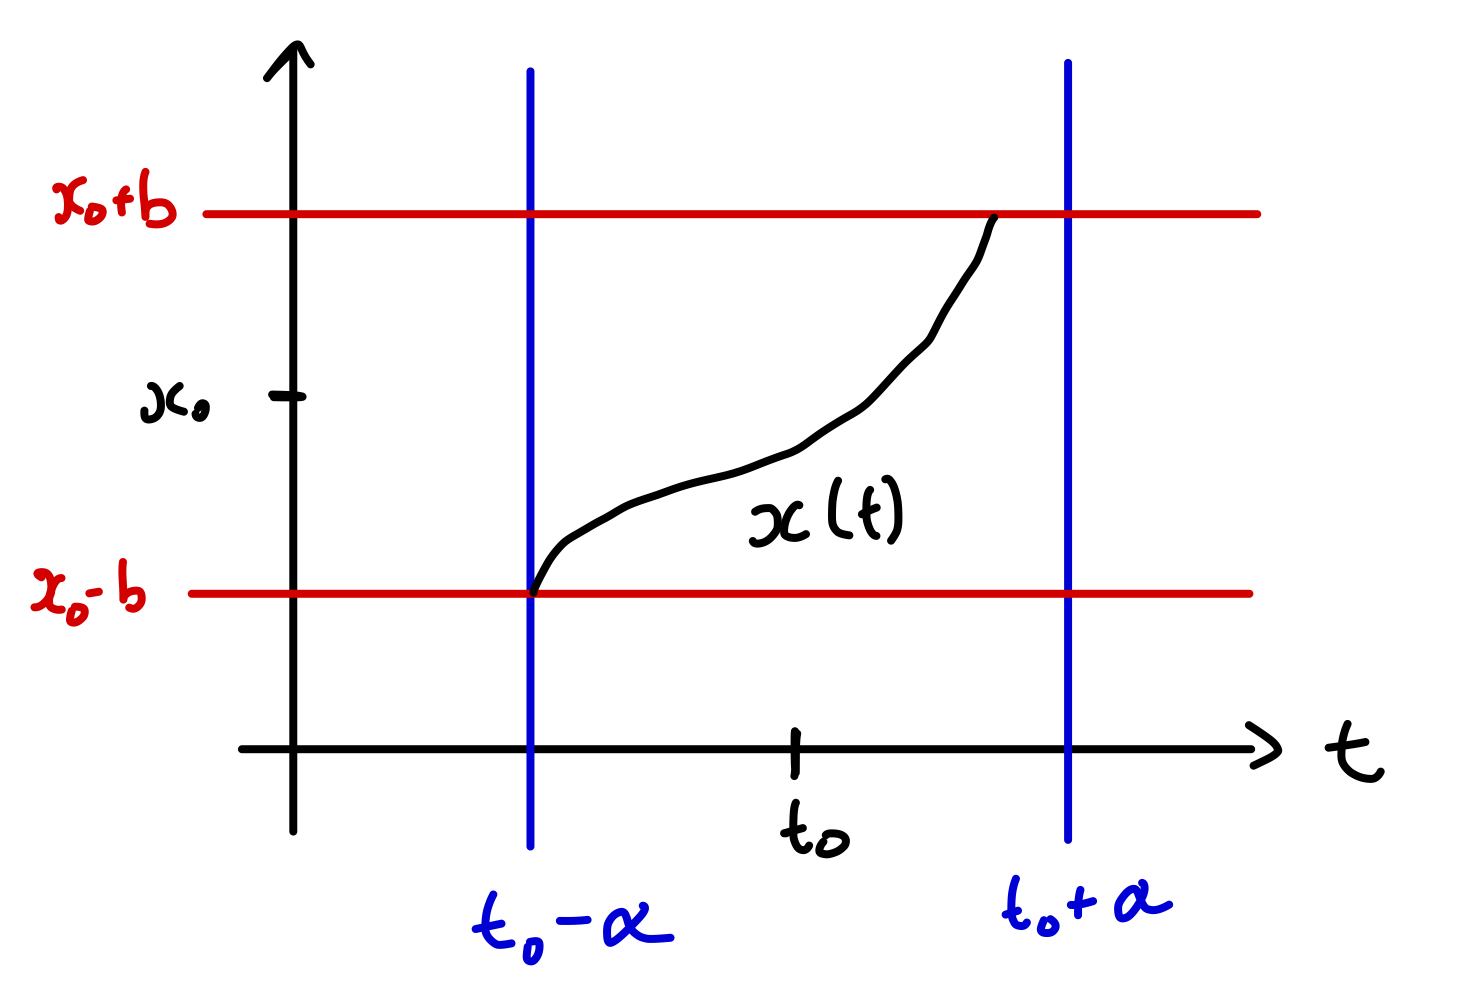
\includegraphics[width=0.3\linewidth]{Bilder/picard.png}
\caption{Auf einer Umgebung von $t_0$ ist das AWP eindeutig lösbar.}
\end{figure}
\end{theorem}
\begin{beweis}
Der Raum $X:= C([t_0 - \alpha, t_0 + \alpha], \overline{B(x_0, b)}$ ist mit der Supremumsnorm ein vollständiger metrischer Raum. Die Menge $Y:= \{ \phi \in X | \phi(t_0)=x_0 \} \sub X$ ist als abgeschlossene Teilmenge auch vollständig.\\
Wir definieren 
\begin{align}
A: Y &\to C([t_0 - \alpha, t_0 + \alpha], \R^n)\\
t &\mapsto (A\phi)(t) := x_0 + \int_{t_0}^t F(\phi(s), s) ds.
\end{align}
Nun zeigt man:
\begin{itemize}
\item $\phi \in Y \implies A\phi \in Y$
\item $A: Y \to Y$ ist eine Kontraktion.
\item Der Fixpunkt von $A$ löst das AWP.
\item Jede Lösung des AWP ist ein Fixpunkt von $A$ $\rightarrow$ Lösung ist eindeutig.
\end{itemize}
\end{beweis}
\begin{beispiel}Lipschitzbedingung\\
Die Lipschitz-Bedingung ist wesentlich für die Eindeutigkeit der Lösung. Betrachte z.B. $\dot{x} = \sqrt{x}$ auf $\R$. Die rechte Seite ist in $x_0 = 0$ stetig, aber nicht lokal lipschitzstetig. Tatsächlich gibt es zwei Lösungen mit $x(0)=0$: $x(t)\equiv 0$ und $x(t)=\frac{t^2}{4}$.
\end{beispiel}
\begin{satz}{Stetige Abhängigkeit}{stetigeabh}
Sei $\Os \in \R^n \times \R$ offen und $F: \Os \to \R^n$ lipschitzstetig mit Konstante $K$. Seien $(x_0, t_0) \in \Os$ und $(x_0^\ast, t_0) \in \Os$ zwei AW mit lokalen Lösungen 
\begin{align}
\phi: [t_0 - \alpha, t_0 + \alpha] &\to \R^n, \ \phi(t_0)=x_0 \\
\phi^\ast: [t_0 - \alpha, t_0 + \alpha] &\to \R^n, \ \phi^\ast(t_0)=x_0^\ast
\end{align}
des AWP.\\
Dann gilt
\begin{equation}
|| \phi(t)-\phi^\ast(t)|| \leq ||x_0-x_0^\ast||\exp(K|t-t_0|).
\end{equation}
Insbesondere folgt aus $x_0^\ast \to x_0$ die gleichmäßige Konvergenz $\phi \to \phi^\ast$ in $C([t_0-\alpha, t_0 + \alpha], \R^n)$.
\end{satz}
\begin{bemerkung}
Analog, aber aufwändiger ist zu zeigen:\\
Ist $F$ von Klasse $C^k$ mit Schranke $\tau$ an die $C^k-Norm$, so erhalten wir $C^k-Abschätzungen$ für $||\phi - \phi^\ast||_{C^k}$. Ist insbesondere $F \in \cinf{\Os}{\R^n}$, so hängen die Lösungen glatt vom AW $x_0$ ab.
\end{bemerkung}
\begin{satz}{Rektifizierungssatz}{rektifizierung}
Ist $F: M \to TM$ ein glattes Vektorfeld und $F_p \neq 0$, so existiert eine offene Umgebung $U \sub M$ von $p$ mit lokalen Koordinaten $(x_1, \dots, x_n)$, sodass $F|_U = \frac{\partial}{\partial x_1}$. Die Lösungen (Integralkurven) von $\dot{x} = \frac{\partial}{\partial x_1}$ haben dann die einfache Form
\begin{equation}
x_1(t)=t+x_1(0), \ x_2(t)=x_2(0), \ \dots, \ x_n(t)=x_n(0).
\end{equation}
Dies ist die \textit{Normalform} des Vektorfeldes.
\end{satz}
\begin{korollar}{Aus Picard-Lindelöf}{auspiclöf}
Unter der Lipschitz-Voraussetzung stimmen zwei lokale Lösungen
\begin{align}
\phi_1: (a_1, b_1) &\to \R^n \\
\phi_2: (a_2, b_2) &\to \R^n
\end{align}
des AWP $\dot{\phi}(t)=F(\phi(t), t), \ \phi(t_0)=x_0 \ (\ast)$ auf $(a_1, b_1) \cap (a_2, b_2)$ überein.
\end{korollar}
\begin{bemerkung}Konstruktion der maximalen Lösung\\
Mit Korollar \ref{auspiclöf} kann man die maximale Lösung von $\dot{\phi}(t)=F(\phi(t), t), \ \phi(t_0)=x_0$ konstruieren, indem man aus der Menge
\begin{equation}
\Ms := \{\phi_i: (a_i, b_i) \to \R^n | i \in I \}
\end{equation}
den maximalen Definitionsbereich $I_{x_0}= \bigcup_{i \in I} (a_i, b_i)$ bestimmt und $\phi: I_{x_0} \to \R^n$ durch $\phi(t) = \phi_i(t)$ definiert, wenn $t \in (a_i, b_i)$.
\end{bemerkung}
\begin{satz}{Satz über die maximale Lösung}{maxlsg}
Sei $\Os \sub \R^n \times \R$ und $F: \Os \to \R^n$ lipschitzstetig bezüglich $x$ auf jeder kompakten Teilmenge $A \sub \Os$.\\
Falls die maximale Lösung $\phi_{x_0}:(a(x_0), b(x_0)) \to \R^n$ des AWP $(\ast)$ die Bedingung $b(x_0) < \infty$ erfüllt, so existiert zu jeder kompakten Teilmenge $A \sub \Os$ ein $t_A < b(x_0)$, sodass für alle $t \in (t_A, b(x_0))$ gilt: $(\phi_{x_0}(t), t) \cancel{\in} A$.
\end{satz}
\begin{bemerkung}
Eine analoge Aussage gilt für $a(x_0) > - \infty$.
\end{bemerkung}
\begin{korollar}{Vollständigkeit von Vektorfeldern}{vollstvf}
Ist $X \in \Gamma (TM)$ ein Vektorfeld mit kompaktem Träger, so sind die maximalen Integralkurven von $X$ auf ganz $\R$ definiert.
\end{korollar}
Jetzt wenden wir uns einigen Lösungsmethoden für Differentialgleichungen in $\R$ zu.
\begin{satz}{Trennung der Variablen}{vartrennung}
Sei $F$ so, dass es sich schreiben lässt als $F(x,t) = f(x) \cdot g(t)$ mit $\dot{x}(t) = f(x) \cdot g(t), \ x(t_0) = x_0$. Wir betrachten zwei Fälle:
\begin{enumerate}
\item Fall: $f(x_0)=0$: $x(t)\equiv x_0$ ist eine auf ganz $\R$ definierte Lösung.
\item Fall: $f(x_0)\neq 0$: Ist $f$ stetig, so gilt $f(x) \neq 0$ in einer Umgebung von $x_0$, also gilt
\begin{equation}
\frac{\dot{x}}{f(x)} = g(t).
\end{equation}
Sei $F(y)$ eine Stammfunktion von $\frac{1}{f(y)}$, d.h. $F'(y) = \frac{1}{f(y)}$. Dann gilt 
\begin{equation}
\frac{d}{dt}F(x(t)) = F'(x(t)) \cdot \dot{x}(t) = \frac{\dot{x}(t)}{f(x(t))}= g(t).
\end{equation}
Durch Integration folgt
\begin{equation}
F(x(t)) = F(x(t_0)) + \int_{t_0}^t g(s) ds.
\end{equation}
Ist $F$ lokal invertierbar, können wir daraus $x$ bestimmen.
\end{enumerate}
\end{satz}
\begin{beispiele}
\begin{enumerate}
\item Betrachte $\dot{x} = - \frac{x}{t}$ mit $x(1)=x_0$. Hier ist $f(x) = x$ und $g(t)=- \frac{1}{t}$.\\
Im 1. Fall ist $x_0=0$, also ist $x(t) \equiv 0$ eine auf ganz $(0, \infty)$ definierte Lösung.\\
Im 2. Fall ist $x_0 \neq 0$, also
\begin{equation}
F(x) = \int_{x_0}^x \frac{1}{f(y)} dy = \int_{x_0}^x \frac{1}{y} dy = \ln \left( \frac{x}{x_0} \right).
\end{equation}
Außerdem gilt
\begin{equation}
\int_1^t g(\tau) d \tau = \int_1^t - \frac{1}{\tau} d\tau = - \ln (t).
\end{equation}
Somit erhalten wir
\begin{equation}
\ln \left( \frac{x}{x_0} \right) = - \ln (t) \iff x(t) = \frac{x_0}{t}.
\end{equation}
Für alle $x_0 \in \R$ ist die maximale Lösung auf ganz $(0, \infty)$ definiert.
\item Betrachte $\dot{x} = x^2, \ x(0)=x_0$.\\
Im 1. Fall gilt $x_0=0$, also ist $x(t)=0$ eine auf ganz $\R$ definierte Lösung.\\
Im 2. Fall gilt $x_0 \neq 0$, also 
\begin{equation}
F(x) = \int_{x_0}^x \frac{1}{y} dy = - \left.\frac{1}{y} \right|_{x_0}^x = \frac{1}{x_0}- \frac{1}{x}.
\end{equation}
Integration liefert $\int_0^t g(\tau) d\tau = t$. Gleichsetzen und Auflösen nach $x(t)$ ergibt:
\begin{equation}
x(t) = \frac{x_0}{1-x_0t}.
\end{equation}
Ist $x_0>0$, so ist die maximale Lösung auf $(-\infty, \frac{1}{x_0})$ definiert, für $x_0<0$ hingegen auf $(\frac{1}{x_0}, \infty)$.
\end{enumerate}
\end{beispiele}
\begin{satz}{Variation der Konstanten}{varkonst}
Sei eine ODE der Form $\dot{x} = p(t)x + q(t)$ mit AWP $x(t_0) = x_0$ gegeben. Eine solche ODE heißt \textbf{lineare Differentialgleichung}.\\
Die Lösung funktioniert schrittweise:
\begin{enumerate}
\item Schritt: Man löst das vereinfachte Problem mit $q \equiv 0$, also $\dot{x}=p(t)x$. Durch Trennung der Variablen erhalten wir $\frac{\dot{x}}{x}=p(t)$. Also gilt
\begin{equation}
\ln (x(t)) = \int p(\tau) d\tau + C^\ast \implies x(t) = C \cdot \exp \left( \int p(\tau) d\tau \right)
\end{equation}
mit $C = \exp(C^\ast)$.
\item Schritt: Für das eigentliche Problem machen wir den Ansatz
\begin{align}
x(t) &= C(t) \cdot \exp \left( \int p(\tau) d \tau \right)\\
\implies \dot{x}(t) &= \underbrace{\dot{C}(t) \exp \left( \int p(\tau) d\tau \right)}_{=q(t)} +p(t) \cdot \underbrace{C(t) \exp \left( \int p(\tau) d\tau \right)}_{=p(t)x(t)}.
\end{align}
Also folgt, dass $\dot{C}(t) = q(t) \exp \left( -\int p(\tau) d\tau \right)$.
\end{enumerate}
\end{satz}
\begin{beispiel}
Wir betrachten den einfachsten Fall mit konstanten Koeffizienten, also $\dot{x}=px+q$ mit $p,q \in \R \exc \{0\}$.
\begin{enumerate}
\item Wir lösen $\dot{x} = px$ und erhalten $x(t) = C \exp(pt)$.
\item $\dot{C}=q\exp(-pt) \implies C(t) = - \frac{q}{p} \exp(-pt) + D$. Einsetzen in den Ansatz liefert
\begin{equation}
x(t) = \left( - \frac{p}{q} \exp(-pt) + D\right)\exp(pt) = D \exp(pt) - \frac{q}{p}.
\end{equation}
$D$ bestimmt sich aus dem Anfangswert $x_0 = x(0) = D-\frac{q}{p} \implies D = x_0 + \frac{p}{q}$. Also lautet die Lösung $x(t) = \left( x_0 + \frac{p}{q}\right) \exp (pt) - \frac{q}{p}.$
\end{enumerate}
\end{beispiel}
\begin{bemerkung}Matrixexponential\\
Für $A \in \text{L}(\R^n, \R^n)$ konvergiert die Reihe
\begin{equation}
\exp(A) := \Sum{k,0,\infty} \frac{A^k}{k!}.
\end{equation}
Also ist $\exp(A)$ auch eine lineare Abbildung $\R^n \to \R^n$, die \textbf{Matrixexponential} genannt wird. Sie hat folgende Eigenschaften:
\begin{itemize}
\item $\exp(0) = \id$
\item $AB = BA \implies \exp(A+B)=\exp(A)\exp(B)$
\item $\exp(A)$ ist invertierbar mit $\left( \exp(A)\right)^{-1} = \exp(-A)$.
\item Sei $B$ invertierbar. dann gilt $\exp(BAB^{-1}) = B \exp(A) B^{-1}$.
\item $\det \exp(A) = \exp (\Tr A)$.
\end{itemize}
\end{bemerkung}
\begin{beispiele}
\begin{enumerate}
\item Sei $A$ von Diagonalgestalt $A = \diag \{\lambda_1, \dots, \lambda_n \}$. Dann gilt $A^k = \diag \{\lambda_1^k, \dots, \lambda_n^k \}$, womit das Matrixexponential die Gestalt $\exp(A) = \diag \{ \exp(\lambda_1^k), \dots, \exp(\lambda_n^k) \}$ hat.
\item $A= \mat{0,1}{0,0}$ ist nilpotent, also $A^2=0$. Damit gilt $\exp(A) = \mat{1,1}{0,1}=\id+ A$. Dies kann man verallgemeinern:\\
Sei $A=\mat{\lambda, \mu}{0,\lambda} = \lambda \id + \mu \mat{0,1}{0,0}$. Dann gilt:
\begin{equation}
\exp(A) = \mat{\exp(\lambda), 0}{0, \exp(\lambda)} \mat{1, \mu}{0,1} = \mat{\exp(\lambda), \mu \exp(\lambda)}{0, \exp(\lambda)}.
\end{equation}
\item Weiterhin gilt für $A = \mat{0,-a}{a,0}$, dass $A^2=\mat{-a^2, 0}{0, -a^2}$, $A^3 = \mat{0, a^3}{-a^3, 0}$, usw.\\
ÜA: $exp(A) = \mat{\cos a, -\sin a}{\sin a, \cos a}$
\end{enumerate}
\end{beispiele}
\begin{satz}{Matrixexponential-Lösung eines AWP}{awpexp}
Das AWP
\begin{align}
\dot{x} &= Ax \ \text{für} \ A \in \text{L}(\R^n, \R^n)\\
x(t_0) &= x_0
\end{align}
hat die eindeutige Lösung
\begin{align}
x: \R &\to \R^n \\
t &\mapsto x(t):=\exp((t-t_0)A)x_0.
\end{align}
\end{satz}
\begin{beweis}
Nachrechnen.
\end{beweis}
\begin{bemerkung}
Konkrete Fälle im $\R^2$.\\
Wie betrachten im Folgenden immer die Jordan-Form der Matrizen.
\begin{enumerate}
\item Fall: $A=\diag \{\lambda_1, \lambda_2 \}$ mit $\lambda_1 \leq \lambda_2$ reell.\\
Für $x(0)=x_0$ ist die Lösung des AWPs aus dem Satz gegeben durch 
\begin{equation}
\cvc{x_1(t), x_2(t)} = \cvc{\exp(t\lambda_1)x_1(0), \exp(t \lambda_2)x_2(0)}
\end{equation}
\begin{figure}[H]
\label{fig:fall1}
\centering
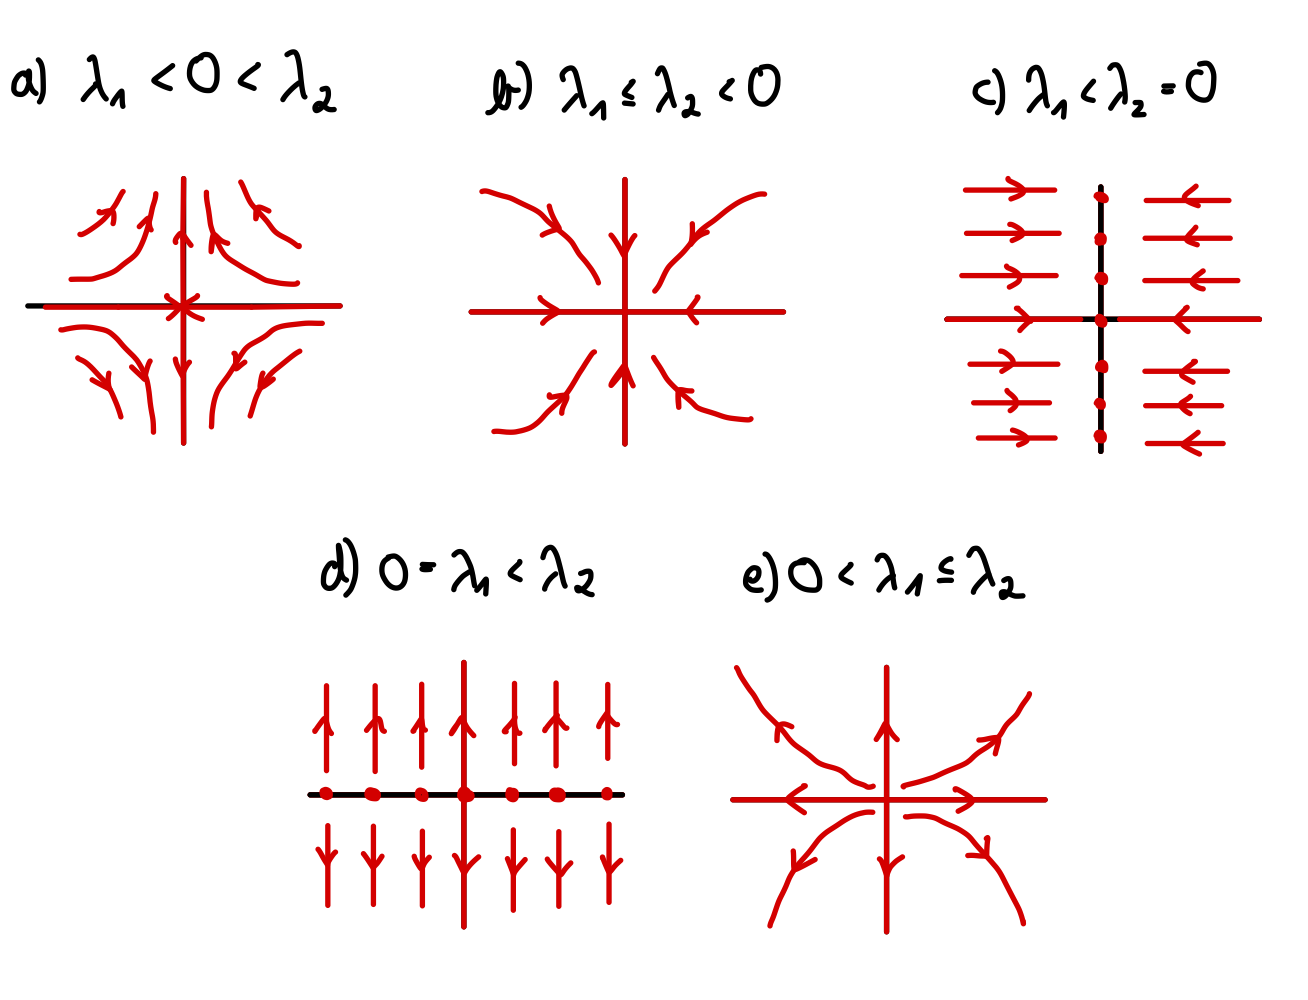
\includegraphics[width=0.5\linewidth]{Bilder/fall1.png}
\end{figure}
\item Fall: $A= \mat{\lambda, 1}{0, \lambda}$, also $\exp(tA) = \mat{\exp(t\lambda), t\exp(t \lambda)}{0, \exp(t\lambda)}$. Dann ist die Lösung gegeben durch
\begin{align}
x_1(t) &= \exp(\lambda t)(x_1(0)+tx_2(0))\\
x_2(t) &= \exp(\lambda t)x_2(0)
\end{align}
\begin{figure}[H]
\label{fig:fall2}
\centering
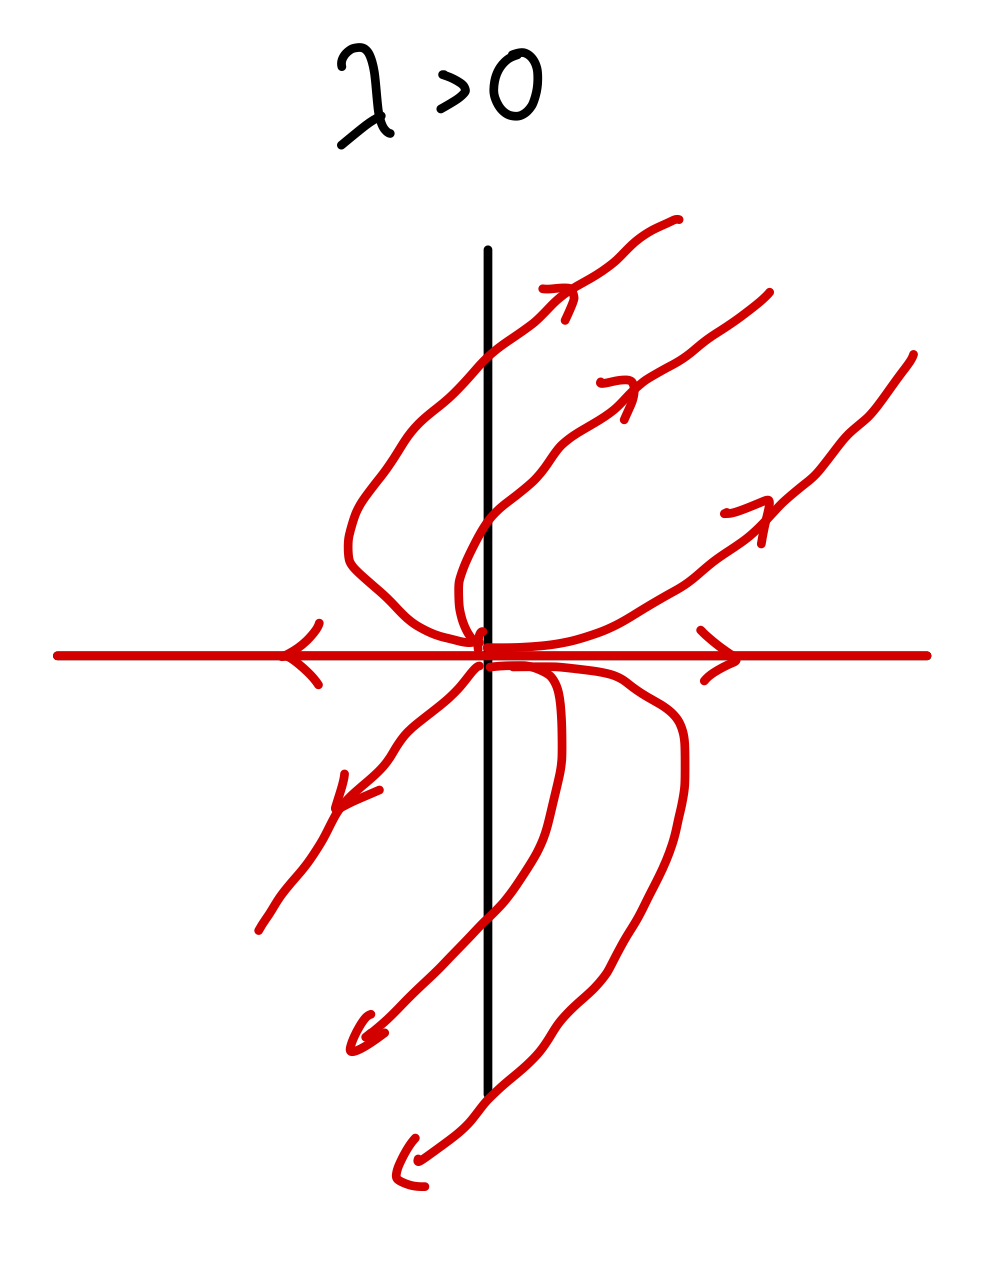
\includegraphics[width=0.2\linewidth]{Bilder/fall2.png}
\end{figure}
\item Fall: $A$ hat zwei komplexe Eigenwerte $\lambda_\pm = a \pm ib$. In einer geeigneten Basis hat $A$ dann die Form
\begin{equation}
A = \mat{a, -b}{b,a} = \mat{a,0}{0,a}+\mat{0,-b}{b,0} = A_1 + A_2.
\end{equation}
Damit gilt
\begin{equation}
\exp(tA) = \exp(tA_1)\exp(tA_2)=\mat{\exp(ta)\cos(b), - \exp(ta) \sin(b)}{\exp(ta) \sin(b), \exp(ta) \cos(b)}.
\end{equation}
\begin{figure}[H]
\label{fig:fall3}
\centering
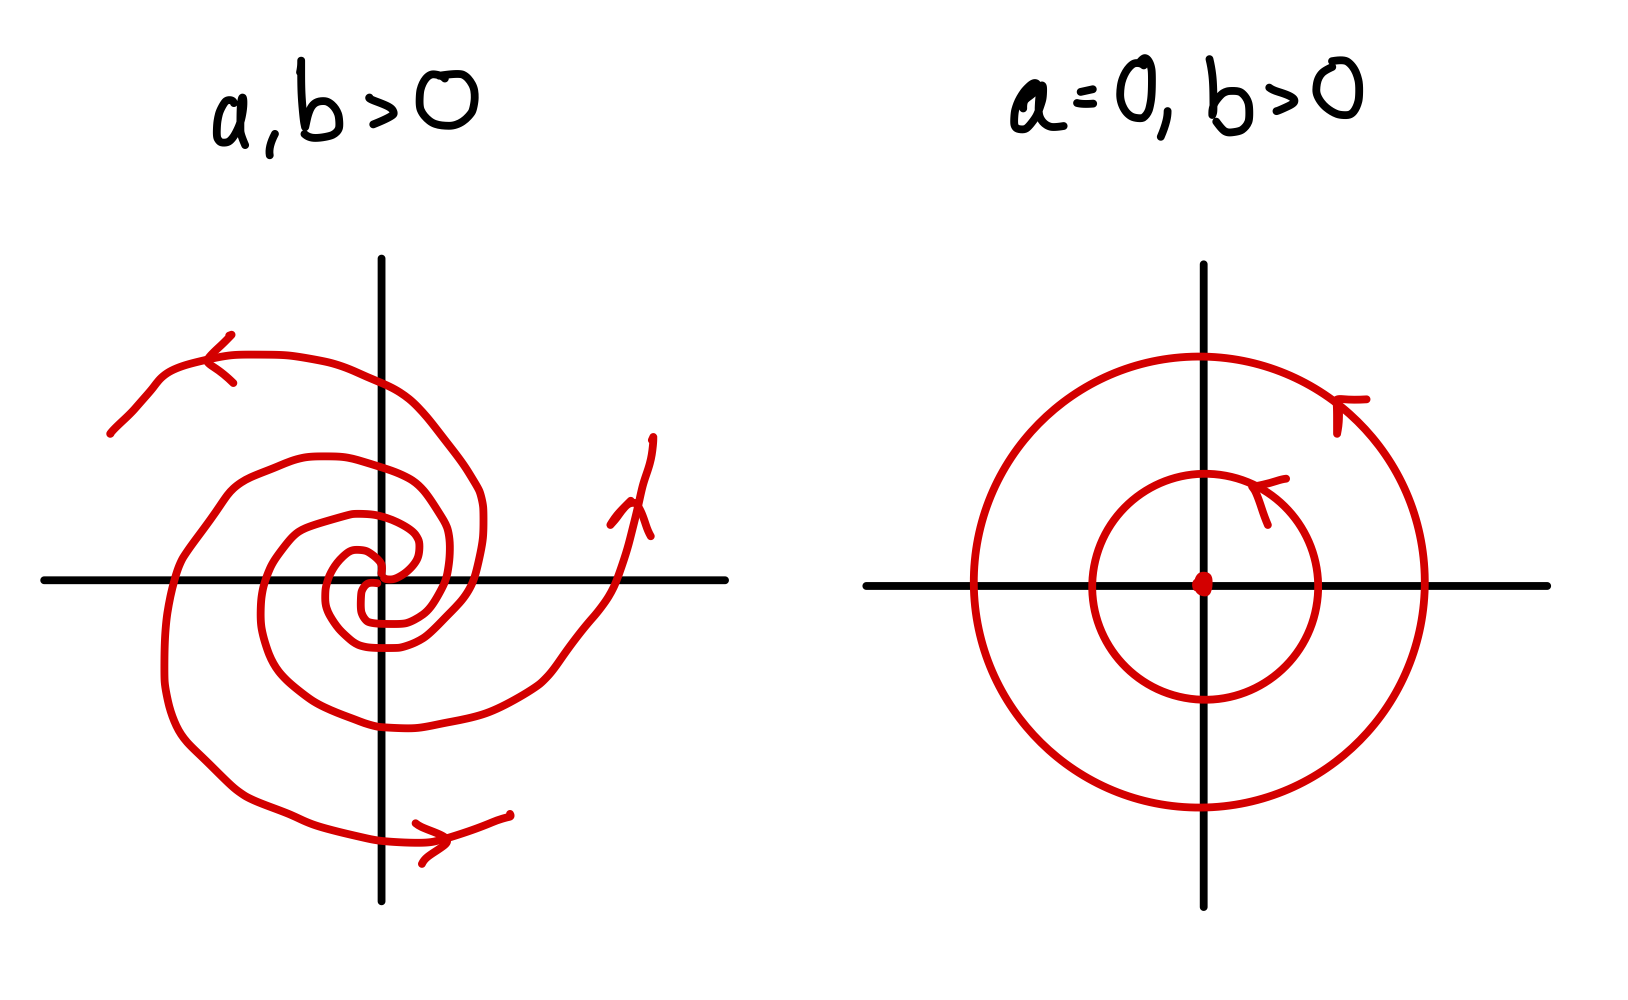
\includegraphics[width=0.3\linewidth]{Bilder/fall3.png}
\end{figure}
\end{enumerate}
\end{bemerkung}
\begin{bemerkung}
Solche linearen DGL sind nützlich für das Studium des qualitativen Verhaltens der Integralkurve eines Vektorfeldes in der Nähe einer isolierten Nullstelle.
\end{bemerkung}
\begin{theorem}{Satz von Grobman-Hartman (Linearisierungssatz)}{grobonanhartman}
Sei $V: \R^n \to \R^n$ ein $\text{C}^1$-Vektorfeld mit $V(0)=0$ und $A := \Ds V_0 \in \text{L}(\R^n, \R^n)$ ohne rein imaginären Eigenwerte.\\
Dann existieren offene Umgebungen $U$ und $U'$ von $0$ und ein \textit{Homöomorphismus} $h: U \to U'$, der Integralkurven von $\dot{x} = V(x)$ in $U$ auf Integralkurven von $\dot{x} = Ax$ in $U'$ abbildet.
\end{theorem}
\begin{beweis}
Geht über den Rahmen der Vorlesung hinaus.
\end{beweis}

\section{Appendix 2: Ein bisschen was für die Physiker...}
\label{ch:physik}
Dieser Abschnitt ist nicht Inhalt der Veranstaltung. Ich habe hier ein paar Definitionen gesammelt, die gewisse Prozesse in der Physik mit den Methoden dieser Vorlesung formalisieren. Dazu folgen wir Lee, Introduction to Riemannian Manifolds und Frankel, The Geometry of Physics.
\subsection{Ricci-Kalkül}
Wir formalisieren ein paar Indexkonventionen aus der Physik.
\begin{definition}{Ricci-Kalkül}
Sei $B^{i_1 \cdots i_r}_{j_1 \cdots j_s}$ ein $(r,s)$-Tensorfeld. Die oberen Indizes $\{i_1, \dots, i_r\}$ heißen \textbf{kontravariante Indizes}, die unteren Indizes $\{j_1, \dots, j_s \}$ heißen \textbf{kovariante Indizes}. Über alle identischen Indizes, die einmal hoch- und einmal tiefgestellt auftauchen, wird summiert:
\begin{equation}
A^\alpha B_\alpha \equiv \sum_\alpha A^\alpha B_\alpha.
\end{equation}
Dies bezeichnet man als \textbf{Einsteinsche Summenkonvention}.\\
Indizes, über die summiert wird, heißen \textbf{Dummy-Indizes}. Alle anderen Indizes heißen \textbf{freie Indizes}.\\
Die partielle Ableitung nach einer Variable $x^\mu$ schreibt man als
\begin{equation}
\frac{\partial}{\partial x^\mu} A_{\alpha \beta \cdots} =: A_{\alpha \beta \cdots, \mu}.
\end{equation}
Die kovariante Ableitung eines Vektorfelds $A^\alpha$ schreibt sich als
\begin{equation}
\nabla_\beta A^\alpha = A^\alpha_{;\beta}.
\end{equation}
Die \textbf{Antisymmetrisierung} von Indizes ist gegeben durch:
\begin{equation}
A_{[\alpha_1 \cdots \alpha_i]\alpha_{i+1} \cdots \alpha_j} = \frac{1}{i!} \sum_\sigma \text{sgn}(\sigma) A_{\alpha_{\sigma(1)} \cdots \alpha_{\sigma(i)} \alpha_{i+1} \cdots \alpha_j}.
\end{equation}
\end{definition}
\begin{bemerkung}
Häufiger werden Indexfamilien mit Großbuchstaben indiziert, um sie übersichtlicher zu machen, also $I = \{i_1, \dots, i_n\}$ bzw. $T^I = T^{i_1 \cdots i_n}$. Ein Pfeil $\underrightarrow{I}$ steht für aufsteigende Ordnung $i_1 < i_2 < \cdots < i_n$ der Indizes.
\end{bemerkung}
\begin{beispiele}
\begin{enumerate}
\item Die Standardkoordinaten sind in dieser Konvention kontravariant, also $\{x\}=(x^1, \dots, x^n)$. Die assoziierten Koordinatenvektorfelder sind hingegen kovariant, also $\{\partial \}=(\partial_1, \dots, \partial_n)$.
\item Sei $V$ ein euklidischer Vektorraum und $V^\ast$ sein Dualraum. Dann schreibt sich ein Vektor $v \in V$ als $v = v^ie_i$ und eine Dualform $f \in V^\ast$ als $f = f_ie^i$. Dabei ist $\{e^i\}$ die Dualbasis zu $\{e_i\}$ mit $e^ie_j = \delta^i_j$.\\
Insbesondere in der Festkörperphysik stellt man die Dualbasis (\textit{Impulsraum}) gerne durch die Basis dar:
\begin{equation}
e^1 = \frac{e_2 \times e_3}{e_1 \cdot (e_2 \times e_3)}, \ e^2= \frac{e_3 \times e_1}{e_2 \cdot (e_3 \times e_1)}, \ e^3 = \frac{e_1 \times e_2}{e_3 \cdot (e_1 \times e_2)}
\end{equation}
\item Auf dem $\R^3$ mit dem Standardskalarprodukt gilt $\langle u, v \rangle = u_iv^i$. Für das Kreuzprodukt gilt hingegen $u \times v = \epsilon^i_{jk} u^j v^k \vec{e}_i$.
\item Für Matrixmultiplikation gilt $(Av)^i = A^i_j v^j$. Die Spur einer Matrix $A^i_j$ reduziert sich zu $A_i^i$.
\item Der Torsionstensor hat in diesem Formalismus die Gestalt 
\begin{equation}
T^\alpha_{\beta \gamma} = \Gamma^\alpha_{\beta \gamma} - \Gamma^\alpha_{\gamma \beta} - \gamma^\alpha_{\beta \gamma}.
\end{equation}
Dabei ist $\gamma^\alpha_{\beta \gamma}$ durch die Lie-Klammer gegeben. Der Riemann-Krümmungstensor hat die Form
\begin{equation}
R^\sigma_{\alpha \beta \gamma} = \Gamma^\sigma_{\gamma \alpha, \beta} - \Gamma^\sigma_{\beta, \alpha, \gamma} + \Gamma^\sigma_{\beta \lambda}\Gamma^\lambda_{\gamma \alpha} - \Gamma^\sigma_{\gamma \lambda}\Gamma^\lambda_{\beta \alpha}.
\end{equation}
Dabei heißen $\Gamma^\alpha_{\beta \gamma}$ \textbf{Christoffel-Symbole der zweiten Art}.
\item Die äußere Ableitung wirkt auf ein total antisymmetrisches $(0,s)$-Tensorfeld, genannt $s$-Form $A_{\alpha_1 \cdots \alpha_s}$. Sie ist gegeben durch:
\begin{equation}
(dA)_{\gamma \alpha_1 \cdots \alpha_s} = A_{[\alpha_1 \cdots \alpha_s, \gamma]}.
\end{equation}
\end{enumerate}
\end{beispiele}
\begin{satz}{Transformationsgesetze für Tensoren}{tensortrafo}
Sei $M$ eine glatte MFK und $T_pM$ der Tangentialraum an $p \in M$. Seien $(x^1, \dots, x^n)$ und $(\bar{x}^1, \dots, \bar{x}^n)$ zwei lokale Rahmen von $T_pM$. Dann gilt für einen $(r,s)$-Tensorfeld folgendes Transformationsgesetz:
\begin{equation}
T^{i'_1 \cdots i'_r}_{j'_1 \cdots j'_s} = \frac{\partial \bar{x}^{i'_1}}{\partial x^{i_1}} \cdots \frac{\partial \bar{x}^{i'_r}}{\partial x^{i_r}}\frac{\partial x^{j_1}}{\partial \bar{x}^{j'_1}} \cdots \frac{\partial x^{j_s}}{\partial \bar{x}^{j'_s}}T^{i_1 \cdots i_r}_{j_1 \cdots j_s} (x^1, \dots, x^n).
\end{equation}
\end{satz}
\begin{definition}{Musikalische Isomorphismen}{musicaliso}
Sei $(M,g)$ eine pseudo-Riemannsche MFK, $\{z_i\}$ ein Rahmen von $TM$ und $\{z^i\}$ der duale Rahmen von $T^\ast M$. Sei weiterhin $X = X^iz_i \in \Gamma(TM)$ ein glattes Vektorfeld und $g^{-1} = g^{ij}$ die inverse Metrik. Dann definiert 
\begin{align}
\flat: TM &\to T^\ast M\\
X &\mapsto X^\flat = g_{ij} X^i z^j = X_j z^j
\end{align}
den \textbf{Flat-Isomorphismus}, für den wir auch $X^\flat(Y)=\langle X, Y \rangle$ mit $Y \in \Gamma(TM)$ schreiben.\\
Sei jetzt $\omega = \omega_iz^i \in \Gamma(T^\ast M)$ eine Dualform. Dann definiert
\begin{align}
\sharp: T^\ast M &\to TM \\
\omega &\mapsto \omega^\sharp = g^{ij}\omega_iz_j = \omega^j z_j
\end{align}
den \textbf{Sharp-Isomorphismus}, kompakter als $\langle \omega^\sharp, Y \rangle = \omega(Y)$ notiert.\\
Beide Isomorphismen heißen zusammen \textbf{musikalische Isomorphismen}.
\end{definition}
\begin{bemerkung}
Sei $A^{i_1 \cdots i_r}_{j_1 \cdots j_s}$ ein $(r,s)$-Tensor. Dann senken wir einen Index $i_n \in \{i_1, \dots, i_r\}$ durch die Wirkung von flat:
\begin{equation}
A^{i_1 \cdots i^\flat_n \cdots i_r}_{j_1 \cdots j_s} = g_{k_ni_n} A^{i_1 \cdots i_n \cdots i_r}_{j_1 \cdots j_s} = A^{i_1 \cdots i_{r-1}}_{j_1 \cdots j_{s} k_{n}}
\end{equation}
und heben einen Index $j_m \in \{j_1, \dots, j_s\}$ durch die Wirkung von sharp:
\begin{equation}
A^{i_1 \cdots i_r}_{j_1 \cdots j^\sharp_m \cdots j_s} = g^{k_mj_m} A^{i_1 \cdots i_r}_{j_1 \cdots j_m \cdots j_s} = A^{i_1 \cdots i_r k_m}_{j_1 \cdots j_s}.
\end{equation}
\end{bemerkung}
\subsection{Hodge-Theorie}
\begin{definition}{Hodge-Stern-Operator}{hodge}
Sei $(M,g)$ eine orientierte, $n$-dimensionale pseudo-Riemannsche MFK und $\omega \in \Omega^k(M)$ eine $k$-Form auf $M$. Dann bezeichnet man den Isomorphismus
\begin{align}
\hodge: \Omega^k(M) &\to \Omega^{n-k} (M)\\
\omega &\mapsto \hodge \omega
\end{align}
als \textbf{Hodge-Stern-Operator}. Dabei ist $\hodge \omega$ als diejenige $(n-k)$-Form eindeutig definiert, für die
\begin{equation}
\eta \wedge \hodge \xi = g(\eta, \xi)\mu
\end{equation}
gilt, wobei $\mu$ die Volumenform auf $M$ ist.
\end{definition}
\begin{satz}{Lokale Darstellung des Hodge-Stern-Operators}{localhodge}
Für Rechnungen ist oftmals eine Formel in lokalen Koordinaten nützlich. Sei dazu $(M,g)$ eine Riemannsche MFK, $\{\partial^1, \dots, \partial^n\}$ eine Basis von $T_pM$ und $\{dx_1, \dots, dx_n\}$ die Dualbasis von $T^\ast_pM$ mit $g_{ij} = \langle \partial^i, \partial^j \rangle$ und $g^{ij} = \langle dx^i, dx^j \rangle$. Dann gilt für eine beliebige $k$-Form:
\begin{equation}
\hodge (dx^{i_1} \wedge \cdots \wedge dx^{i_k}) = \frac{\sqrt{|\det g|}}{(n-k)!} g^{i_1j_1} \dots g^{i_kj_k} \epsilon_{j_1 \cdots j_n} dx^{j_{k+1}} \wedge \cdots \wedge dx^{j_n}.
\end{equation}
\end{satz}
\begin{definition}{Kodifferential}{kodifferential}
Sei $(M,g)$ eine pseudo-Riemannsche MFK der Dimension $n$ mit Signatur $\mathfrak{s} \in \Z$ und $\omega \in \Omega^k(M)$. Dann heißt die Abbildung
\begin{align}
\delta: \Omega^k(M) &\to \Omega^{k-1}\\
\omega &\mapsto \delta \omega =  (-1)^{n(k+1)+1} \mathfrak{s} \ \hodge d \hodge \omega.
\end{align}
\textbf{Kodifferential}.
\end{definition}
\begin{bemerkungen}
\begin{enumerate}
\item Das Kodifferential ist dual zur äußeren Ableitung: $\langle \eta, \delta \xi \rangle_{L^2} = \langle d\eta, \xi \rangle_{L^2}$.
\item Das Kodifferential hat auch die Eigenschaft $\delta^2 = 0$.
\end{enumerate}
\end{bemerkungen}
\begin{beispiele}
\begin{enumerate}
\item Wir betrachten $\R^3$ mit der Standardmetrik. Dann gilt:
\begin{align}
\hodge dx &= dy \wedge dz\\
\hodge dy &= dz \wedge dx\\
\hodge dz &= dx \wedge dy.
\end{align}
Damit folgt insbesondere $\hodge (u \wedge v) = u \times v$ und $\hodge (u \times v) = u \wedge v$ für $u,v \in \R^3$.
\item Auf $\R^3$ gilt 
\begin{equation}
df = \frac{\partial f}{\partial x} dx + \frac{\partial f}{\partial y} dy + \frac{\partial f}{\partial z} dz \equiv \left(\frac{\partial f}{\partial x},  \frac{\partial f}{\partial y},\frac{\partial f}{\partial z} \right) = \text{grad} \ f
\end{equation}
Ein Vektorfeld $X = X^1 dx + X^2 dy + X^3 dz$ lässt sich so als $1$-Form schreiben. Dann gilt:
\begin{equation}
dX = \left(\frac{\partial X^3}{dy} - \frac{\partial X^2}{dz} \right) dy \wedge dz + \left(\frac{\partial X^3}{dx} - \frac{\partial X^1}{dz} \right) dx \wedge dz + \left(\frac{\partial X^2}{dx} - \frac{\partial X^1}{dy} \right) dx \wedge dy
\end{equation}
und damit
\begin{equation}
\hodge dX =  \left(\frac{\partial X^3}{dy} - \frac{\partial X^2}{dz} \right) dx - \left(\frac{\partial X^3}{dx} - \frac{\partial X^1}{dz} \right) dy + \left(\frac{\partial X^2}{dx} - \frac{\partial X^1}{dy} \right) dz \equiv \text{rot} \ X.
\end{equation}
Weiterhin folgt
\begin{equation}
\delta X = \hodge d \hodge X = \frac{\partial X^1}{\partial x} + \frac{\partial X^2}{\partial y} + \frac{\partial X^3}{\partial z} = \text{div} \ X.
\end{equation}
Also sind die Operatoren der Divergenz, der Rotation und des Gradienten nichts anderes als spezielle Differentialformen in $\R^3$. Durch die Identität $d^2=0$ kann man sofort mehrere Eigenschaften der Operatoren herleiten.
\end{enumerate}
\end{beispiele}
\begin{bemerkungen}
\begin{enumerate}
\item Die Volumenform lässt sich durch den Hodge-Stern-Operator als $\mu = \hodge 1$ auffassen mit
\begin{equation}
\mu = \sqrt{|\det g|} dx^1 \wedge \cdots \wedge dx^n.
\end{equation}
\item Damit sehen wir für das Integral über $M$ die Formel
\begin{equation}
\int_M \eta \wedge \hodge \xi = \int_M \langle \eta, \xi \rangle \mu.
\end{equation}
\item Die \textbf{Maxwell-Gleichungen} lassen sich nun von vier auf zwei Gleichungen reduzieren. Sei $E$ das elektrische Feld, $B$ das magnetische Feld, $c$ die Lichtgeschwindigkeit, $\rho$ die Ladungsdichte, $\epsilon_0$ die Permittivität des Vakuums, $\mu_0$ die Permeabilität des Vakuums und $J$ der Strom. Dann gilt:
\begin{align}
1.& \ d \hodge E = \frac{\rho}{\epsilon_0}\\
2.& \ d \hodge B - \frac{1}{c^2} \frac{\partial \hodge E}{\partial t} = \mu_0 J.
\end{align}
\item Sei nun $F_{\alpha \beta}$ der elektromagnetische Feldstärketensor und $J^\alpha$ das Viererstrom-Vektorfeld. Die Metrik ist gegeben durch die Minkowski-Metrik $\eta_{\alpha \beta} = \diag (1,-1,-1,-1)$. Dann genügt bereits eine Maxwell-Gleichung:
\begin{equation}
d \hodge F = \mu_0 J.
\end{equation}
\end{enumerate}
\end{bemerkungen}
\begin{definition}{Laplace-deRham-Operator}{laplacederham}
Der \textbf{Laplace-DeRham-Operator} ist gegeben durch:
\begin{equation}
\Delta = (\delta + d)^2 = \delta d + d \delta.
\end{equation}
Es handelt sich um einen verallgemeinerten Laplace-Operator.
\end{definition}
\end{document}